% $Id: msk-014-prog.tex 9791 2022-01-24 05:15:58Z mskala $

%
% MSK 014 programmer's manual
% Copyright (C) 2022  Matthew Skala
%
% This program is free software: you can redistribute it and/or modify
% it under the terms of the GNU General Public License as published by
% the Free Software Foundation, version 3.
%
% This program is distributed in the hope that it will be useful,
% but WITHOUT ANY WARRANTY; without even the implied warranty of
% MERCHANTABILITY or FITNESS FOR A PARTICULAR PURPOSE.  See the
% GNU General Public License for more details.
%
% You should have received a copy of the GNU General Public License
% along with this program.  If not, see <http://www.gnu.org/licenses/>.
%
% Matthew Skala
% https://northcoastsynthesis.com/
% mskala@northcoastsynthesis.com
%

\documentclass{ncmanual}

% \usepackage{bigstrut}
% \usepackage{dcolumn}
\usepackage{musicography}
% \usepackage{rotating}
% \usepackage{stfloats}
\usepackage{tikz}

\usetikzlibrary{arrows.meta,calc,shapes}

\title{MSK~014\quad Gracious Host\\Programmer's Manual}
\author{Matthew Skala}
\date{\today}

\newcommand{\insn}[1]{\textbf{#1}}

\begin{document}

\maketitle

%%%%%%%%%%%%%%%%%%%%%%%%%%%%%%%%%%%%%%%%%%%%%%%%%%%%%%%%%%%%%%%%%%%%%%%%

\begin{copyrightpage}
Software documentation for the MSK~014\\
Copyright \copyright\ 2022 Matthew Skala

\GPLThreeStatement
\end{copyrightpage}

\tableofcontents

%%%%%%%%%%%%%%%%%%%%%%%%%%%%%%%%%%%%%%%%%%%%%%%%%%%%%%%%%%%%%%%%%%%%%%%%

\texdependspdfworkaround

% $Id: introduction.tex 9826 2022-02-09 20:05:05Z mskala $

%
% MSK 014 programmer's manual introduction
% Copyright (C) 2022  Matthew Skala
%
% This program is free software: you can redistribute it and/or modify
% it under the terms of the GNU General Public License as published by
% the Free Software Foundation, version 3.
%
% This program is distributed in the hope that it will be useful,
% but WITHOUT ANY WARRANTY; without even the implied warranty of
% MERCHANTABILITY or FITNESS FOR A PARTICULAR PURPOSE.  See the
% GNU General Public License for more details.
%
% You should have received a copy of the GNU General Public License
% along with this program.  If not, see <http://www.gnu.org/licenses/>.
%
% Matthew Skala
% https://northcoastsynthesis.com/
% mskala@northcoastsynthesis.com
%

\chapter{Introduction}

This manual documents the MSK~014 Gracious Host from a programmer's
perspective.  The Gracious Host is a module for use in a Eurorack modular
synthesizer, with the main function of interfacing USB MIDI controller
devices to CV/gate synthesizer patches.  It can be programmed in the field
with alternate firmware, potentially allowing an unlimited range of other
functions, and this manual is intended for programmers interested in
creating alternate firmware, modifying the standard firmware, or studying
how it works.

Writing software for the Gracious Host requires many skills, and a deep
understanding of software and hardware engineering issues that are not taught
in this manual.  This is primarily a reference for qualified programmers,
not a tutorial.  Most users of the module will not be well served by
attempting to modify the firmware themselves, and would do better to read
the \emph{MSK~014 Gracious Host User/Build Manual} (UBM) instead of this
one.  This manual assumes knowledge of the material included there.  You
will also need the manuals, data sheets, and errata published by Microchip
Corporation for the PIC24F microcontroller family; the PIC24FJ64GB002 chip
in particular; the other chips on the board; the assembler and linker (both
the software tools and the manuals for them); and so on.

\section{This manual's organization}

After this introduction, there are a couple of chapters describing the
hardware; then the bulk of the manual is about the standard firmware,
structured as a chapter on tools and building, one on code conventions and
programming tips, then a chapter for each major source file.  The source
chapters are arranged by increasing abstraction level from basic services
close to the hardware, through core subsystems like the USB host driver and
MIDI backend, and finally to the per-device USB drivers, which are basically
applications running on top of the core subsystems.  The manual ends with a
glossary mostly focused on expanding the (many) abbreviations used in my and
Microchip's documentation.  Most all-caps abreviations including TLAs, and
many terms used in \emph{italics}, are defined in the glossary.

Assembly language instructions are printed in lowercase bold, like
\insn{nop}.  Prefix 0x indicates hexadecimal and other numbers are decimal,
as in 0xF00 = 3840.

\section{A note on standards}

The Gracious Host is intended to work with USB and MIDI devices but it is
not a compliant implementation of the associated standards.  Both USB and
MIDI are managed by industry organizations who attempt to enforce rules on,
and collect high membership fees from, companies who use their trademarks or
advertise standards compliance.  As such, it would be inadvisable to use the
trademarked logos of those organizations in connection with the Gracious
Host.

\section{Use and contact information}

This module design, including the firmware described in this manual, is
released under the GNU GPL, version 3, a copy of which is in the source code
package in the file named \texttt{COPYING}.  One important consequence of
the license is that if you create new firmware incorporating parts of my
standard firmware and you distribute the modified firmware in binary form --
for instance, as a loadable firmware image or loaded into a Gracious Host
module -- then you are obliged to make the source code available to
whoever gets the binary.  You are not permitted to limit others' freedoms to
redistribute the code and make further modifications of their own.

I sell the Gracious Host and other modules, both as fully assembled products
and do-it-yourself kits, from my Web storefront at
\url{https://northcoastsynthesis.com/}.  Your support of my business is what
makes it possible for me to continue releasing module designs for free.  The
latest version of this document and the associated source files can be found
at that Web site.

Email should be sent to\\ \url{mskala@northcoastsynthesis.com}.

% $Id: onchip.tex 9826 2022-02-09 20:05:05Z mskala $

%
% Manual for MSK 014 on-chip peripherals
% Copyright (C) 2022  Matthew Skala
%
% This program is free software: you can redistribute it and/or modify
% it under the terms of the GNU General Public License as published by
% the Free Software Foundation, version 3.
%
% This program is distributed in the hope that it will be useful,
% but WITHOUT ANY WARRANTY; without even the implied warranty of
% MERCHANTABILITY or FITNESS FOR A PARTICULAR PURPOSE.  See the
% GNU General Public License for more details.
%
% You should have received a copy of the GNU General Public License
% along with this program.  If not, see <http://www.gnu.org/licenses/>.
%
% Matthew Skala
% https://northcoastsynthesis.com/
% mskala@northcoastsynthesis.com
%

\chapter{On-chip peripherals}

The PIC24FJ64GB002 chip has a large assortment of built-in peripherals. 
This chapter summarizes how all the peripherals are used (if at all) in the
Gracious Host.

Microchip's documentation is a little weird.  They make many different
PIC24F chips, all with different selections of peripherals and different
details of how the peripherals can be configured.  There is the so-called
\emph{Data Sheet} (DS), which is hundreds of pages long, not really a
``sheet'' at all, for the PIC24FJ64GB002 chip.  Actually, it is for the
PIC24FJ64GB004; the -002 is a sort of poor cousin, covered by the same data
sheet.  Then there is also a \emph{Family Reference Manual} (FRM) for the
entire PIC24F family.  That describes the union of all the peripherals on
all chips in the PIC24F family.  It gives programming details for each
peripheral that are not included in the DS, so you need to read the FRM to
really write code for each peripheral; but you also need to read the DS for
specific per-chip information like how many of each kind of timer there are
and the addresses of the registers in data memory.

The chip is also old enough that it can be hard to find the correct versions
of some of the documentation on the Net.  In particular, be sure not to
confuse chapters of the PIC24F FRM with the ``dsPIC'' FRM; incautious search
engine queries are likely to return a mixture of the two.  The PIC24F FRM
does not appear to be available as a single document, and Microchip does not
make it easy to find.  You need to search for specific chapters by number. 
The DS is still readily available on their Web site.

I will go through all the chapters of the DS, describing the specific
considerations relevant to that part of the hardware in the context of the
Gracious Host.  Notes like ``(DS 3, FRM 2)'' refer to the relevant
chapter numbers in the \emph{Data Sheet} and \emph{Family Reference Manual}. 
Not every item is covered in both manuals.  In addition to these sources it
is also important to be aware of Microchip's published silicon errata; I
mention those in this summary wherever they have an impact on the Gracious
Host.

%%%%%%%%%%%%%%%%%%%%%%%%%%%%%%%%%%%%%%%%%%%%%%%%%%%%%%%%%%%%%%%%%%%%%%%%

\section{Device overview (DS 1)}

The first chapter of the DS just gives a high-level description of the
features on the chip, and describes the pinouts of the different package
variations.  Note we are using the 28-pin SPDIP.

Many pins on the microcontroller chip are general-purpose I/O (GPIO) pins
that can be reassigned to special functions with the Peripheral Pin Select
(PPS) system.  Even if left generic in the microcontroller configuration,
all 28 pins have specific purposes in the Gracious Host hardware.  So
Table~\ref{tab:mpu-pinout} gives a more specific pinout, showing the names
used by Microchip's documentation as well as the net names used in my
schematic, as well as notes on how the pins are used.  For more details of the
wiring, see the UBM with its schematics and circuit
descriptions.

\begin{table*}
{\centering
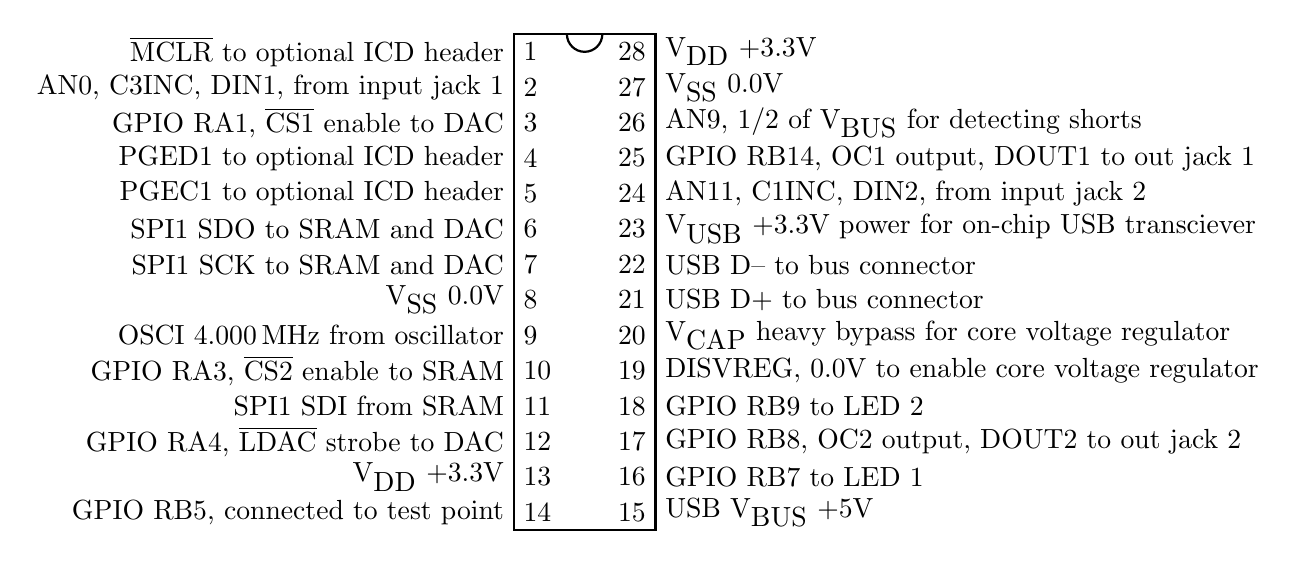
\begin{tikzpicture}[scale=4.5]
  \draw[thick] (-0.2,0.05) rectangle (0.2,-1.35);
  \draw[thick] (-0.05,0.05) arc[radius=0.05,start angle=180,end angle=360];
  \foreach \y in {1,...,14} {
    \node[anchor=west] at (-0.2,0.1-0.1*\y) {\y};
  }
  \foreach \y in {15,...,28} {
    \node[anchor=east] at (0.2,-2.8+0.1*\y) {\y};
  }
  \node[anchor=east] at (-0.2,0.0)
    {$\overline{\textrm{MCLR}}$ to optional ICD header};
  \node[anchor=east] at (-0.2,-0.1)
    {AN0, C3INC, DIN1, from input jack 1};
  \node[anchor=east] at (-0.2,-0.2)
    {GPIO RA1, $\overline{\textrm{CS1}}$ enable to DAC};
  \node[anchor=east] at (-0.2,-0.3)
    {PGED1 to optional ICD header};
  \node[anchor=east] at (-0.2,-0.4)
    {PGEC1 to optional ICD header};
  \node[anchor=east] at (-0.2,-0.5)
    {SPI1 SDO to SRAM and DAC};
  \node[anchor=east] at (-0.2,-0.6)
    {SPI1 SCK to SRAM and DAC};
  \node[anchor=east] at (-0.2,-0.7)
    {V$_\textrm{SS}$ 0.0V};
  \node[anchor=east] at (-0.2,-0.8)
    {OSCI 4.000\,MHz from oscillator};
  \node[anchor=east] at (-0.2,-0.9)
    {GPIO RA3, $\overline{\textrm{CS2}}$ enable to SRAM};
  \node[anchor=east] at (-0.2,-1.0)
    {SPI1 SDI from SRAM};
  \node[anchor=east] at (-0.2,-1.1)
    {GPIO RA4, $\overline{\textrm{LDAC}}$ strobe to DAC};
  \node[anchor=east] at (-0.2,-1.2)
    {V$_\textrm{DD}$ +3.3V};
  \node[anchor=east] at (-0.2,-1.3)
    {GPIO RB5, connected to test point};
  \node[anchor=west] at (0.2,-1.3)
    {USB V$_\textrm{BUS}$ +5V};
  \node[anchor=west] at (0.2,-1.2)
    {GPIO RB7 to LED 1};
  \node[anchor=west] at (0.2,-1.1)
    {GPIO RB8, OC2 output, DOUT2 to out jack 2};
  \node[anchor=west] at (0.2,-1.0)
    {GPIO RB9 to LED 2};
  \node[anchor=west] at (0.2,-0.9)
    {DISVREG, 0.0V to enable core voltage regulator};
  \node[anchor=west] at (0.2,-0.8)
    {V$_\textrm{CAP}$ heavy bypass for core voltage regulator};
  \node[anchor=west] at (0.2,-0.7)
    {USB D+ to bus connector};
  \node[anchor=west] at (0.2,-0.6)
    {USB D-- to bus connector};
  \node[anchor=west] at (0.2,-0.5)
    {V$_\textrm{USB}$ +3.3V power for on-chip USB transciever};
  \node[anchor=west] at (0.2,-0.4)
    {AN11, C1INC, DIN2, from input jack 2};
  \node[anchor=west] at (0.2,-0.3)
    {GPIO RB14, OC1 output, DOUT1 to out jack 1};
  \node[anchor=west] at (0.2,-0.2)
    {AN9, 1/2 of V$_\textrm{BUS}$ for detecting shorts};
  \node[anchor=west] at (0.2,-0.1)
    {V$_\textrm{SS}$ 0.0V};
  \node[anchor=west] at (0.2,-0.0)
    {V$_\textrm{DD}$ +3.3V};
\end{tikzpicture}\par}
\caption{Microcontroller pinout.}\label{tab:mpu-pinout}
\end{table*}

See Table~\ref{tab:timers} for an overview of how the Gracious Host
firmware configures many of its on-chip peripherals and which source files
do that.  The rectangular boxes show where the peripherals get their
configuration registers initialized -- sometimes more than one place if
different software modules reinitialize the peripherals -- even if the
peripherals end up being accessed elsewhere, as noted.  The oval ISR
notations show where the hard interrupt vectors point.  The ADC and output
compare hardware depends on clock frequencies that come from Timer~3 and its
prescaler, and the ISR for the comparator interrupts depends on reading time
values from Timers~4 and~5.  All the general-purpose timers are configured
to take their input from the 16.000\,MHz instruction clock.  Some other
peripherals that are less heavily linked to others, like the USB subsystem,
are not shown in this table.

\begin{table*}
{\centering
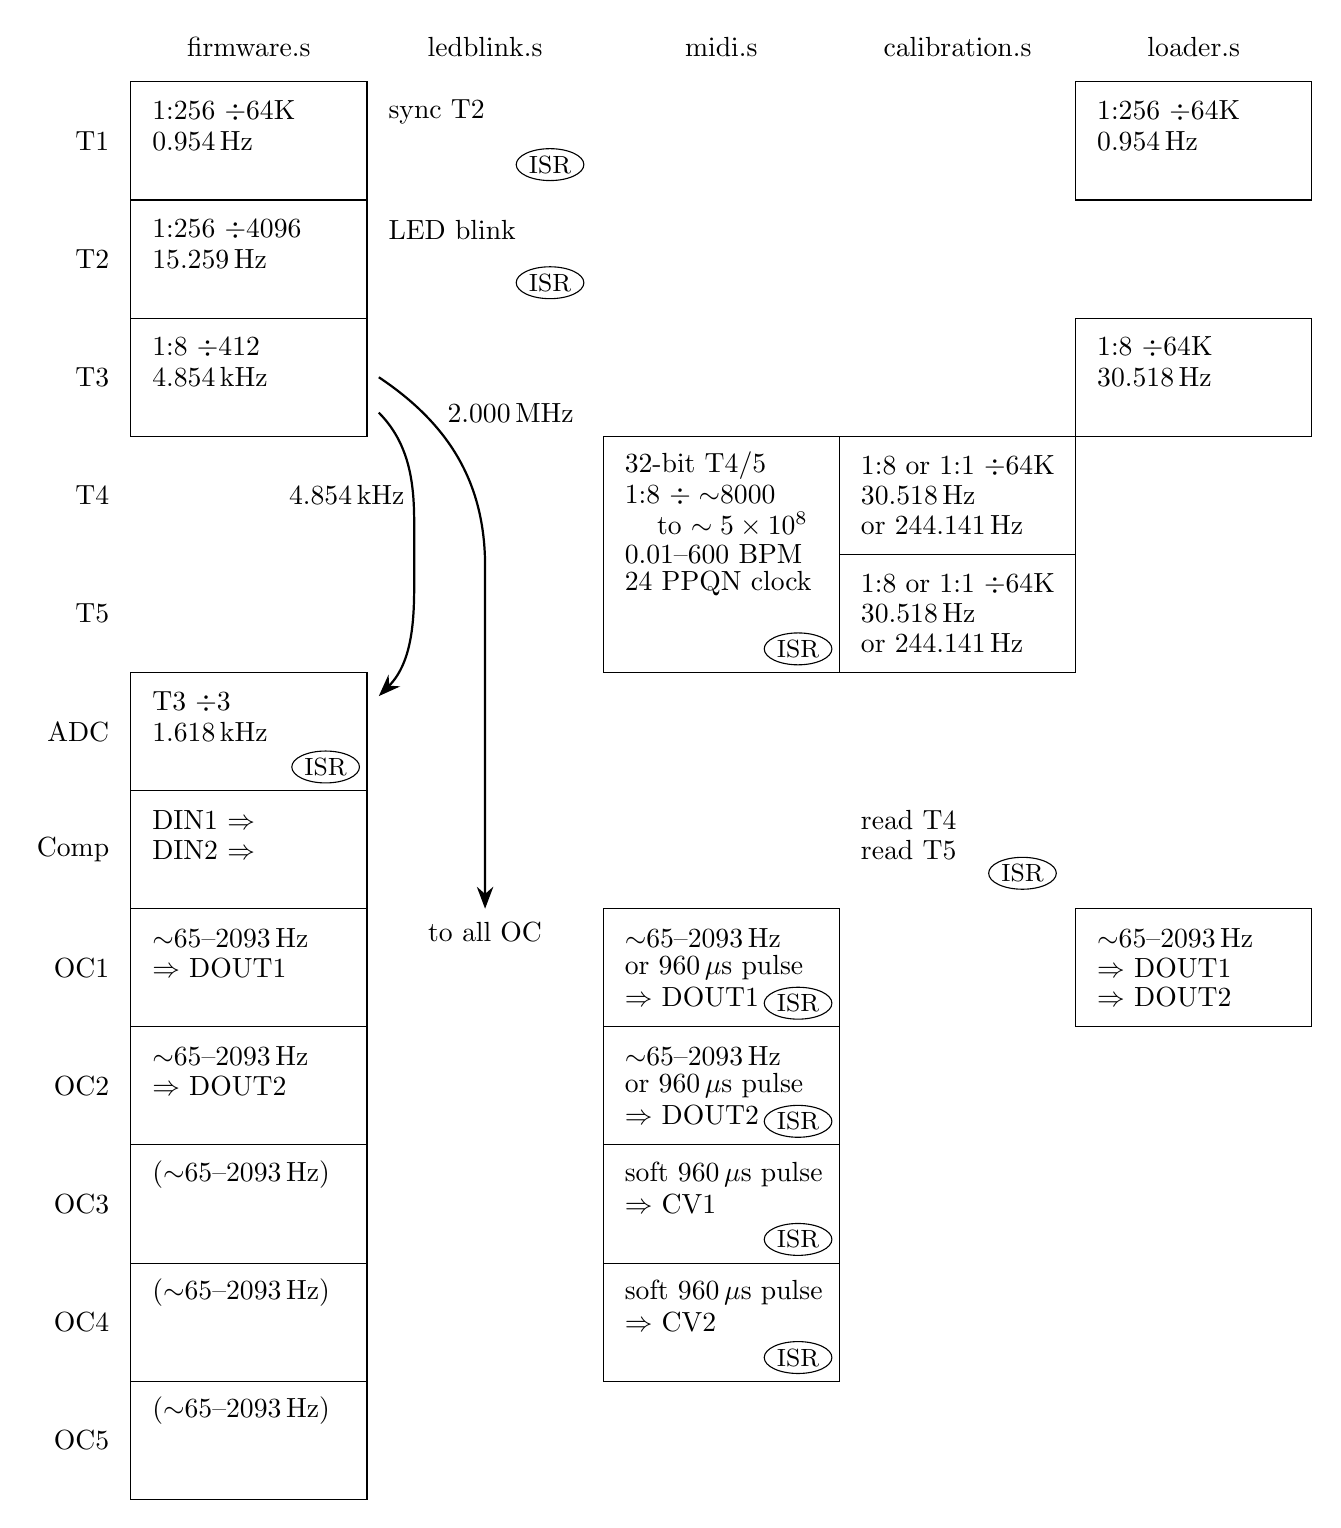
\begin{tikzpicture}[scale=1.5]
  \node at (1,0.3) {firmware.s};
  \node at (3,0.3) {ledblink.s};
  \node at (5,0.3) {midi.s};
  \node at (7,0.3) {calibration.s};
  \node at (9,0.3) {loader.s};
%
  \node[anchor=east] at (-0.1,-0.5) {T1};
  \node[anchor=east] at (-0.1,-1.5) {T2};
  \node[anchor=east] at (-0.1,-2.5) {T3};
  \node[anchor=east] at (-0.1,-3.5) {T4};
  \node[anchor=east] at (-0.1,-4.5) {T5};
  \node[anchor=east] at (-0.1,-5.5) {ADC};
  \node[anchor=east] at (-0.1,-6.5) {Comp};
  \node[anchor=east] at (-0.1,-7.5) {OC1};
  \node[anchor=east] at (-0.1,-8.5) {OC2};
  \node[anchor=east] at (-0.1,-9.5) {OC3};
  \node[anchor=east] at (-0.1,-10.5) {OC4};
  \node[anchor=east] at (-0.1,-11.5) {OC5};
%
  \draw (0,-3) rectangle (2,0);
  \draw (0,-1) -- (2,-1);
  \draw (0,-2) -- (2,-2);
  \draw (8,-1) rectangle (10,0);
  \draw (8,-3) rectangle (10,-2);
  \draw (4,-5) rectangle (8,-3);
  \draw (6,-5) -- (6,-3);
  \draw (6,-4) -- (8,-4);
  \draw (0,-12) rectangle (2,-5);
  \draw (0,-6) -- (2,-6);
  \draw (0,-7) -- (2,-7);
  \draw (0,-8) -- (2,-8);
  \draw (0,-9) -- (2,-9);
  \draw (0,-10) -- (2,-10);
  \draw (0,-11) -- (2,-11);
  \draw (4,-11) rectangle (6,-7);
  \draw (8,-8) rectangle (10,-7);
  \draw (4,-8) -- (6,-8);
  \draw (4,-9) -- (6,-9);
  \draw (4,-10) -- (6,-10);
%
  \node[anchor=west] at (0.1,-0.25) {1:256 $\div$64K};
  \node[anchor=west] at (0.1,-0.5) {0.954\,Hz};
  \node[anchor=west] at (2.1,-0.25) {sync T2};
  \node[anchor=west] at (8.1,-0.25) {1:256 $\div$64K};
  \node[anchor=west] at (8.1,-0.5) {0.954\,Hz};
  \node[anchor=west] at (0.1,-1.25) {1:256 $\div$4096};
  \node[anchor=west] at (0.1,-1.5) {15.259\,Hz};
  \node[anchor=west] at (2.1,-1.25) {LED blink};
  \node[anchor=west] at (0.1,-2.25) {1:8 $\div$412};
  \node[anchor=west] at (0.1,-2.5) {4.854\,kHz};
  \node[anchor=west] at (8.1,-2.25) {1:8 $\div$64K};
  \node[anchor=west] at (8.1,-2.5) {30.518\,Hz};
  \node[anchor=west] at (6.1,-3.25) {1:8 or 1:1 $\div$64K};
  \node[anchor=west] at (6.1,-3.5) {30.518\,Hz};
  \node[anchor=west] at (6.1,-3.75) {or 244.141\,Hz};
  \node[anchor=west] at (6.1,-4.25) {1:8 or 1:1 $\div$64K};
  \node[anchor=west] at (6.1,-4.5) {30.518\,Hz};
  \node[anchor=west] at (6.1,-4.75) {or 244.141\,Hz};
  \node[anchor=west] at (4.1,-3.25) {32-bit T4/5};
  \node[anchor=west] at (4.1,-3.5) {1:8 $\div\sim$8000};
  \node[anchor=west] at (4.1,-3.75) {~~~\,to $\sim5\times10^8$};
  \node[anchor=west] at (4.1,-4.0) {0.01--600 BPM};
  \node[anchor=west] at (4.1,-4.25) {24 PPQN clock};
  \node[anchor=west] at (0.1,-5.25) {T3 $\div$3};
  \node[anchor=west] at (0.1,-5.5) {1.618\,kHz};
  \node[anchor=west] at (0.1,-6.25) {DIN1 $\Rightarrow$};
  \node[anchor=west] at (0.1,-6.5) {DIN2 $\Rightarrow$};
  \node[anchor=west] at (6.1,-6.25) {read T4};
  \node[anchor=west] at (6.1,-6.5) {read T5};
  \node[anchor=west] at (0.1,-7.25) {$\sim$65--2093\,Hz};
  \node[anchor=west] at (0.1,-7.5) {$\Rightarrow$ DOUT1};
  \node[anchor=west] at (4.1,-7.25) {$\sim$65--2093\,Hz};
  \node[anchor=west] at (4.1,-7.5) {or 960\,$\mu$s pulse};
  \node[anchor=west] at (4.1,-7.75) {$\Rightarrow$ DOUT1};
  \node[anchor=west] at (8.1,-7.25) {$\sim$65--2093\,Hz};
  \node[anchor=west] at (8.1,-7.5) {$\Rightarrow$ DOUT1};
  \node[anchor=west] at (8.1,-7.75) {$\Rightarrow$ DOUT2};
  \node[anchor=west] at (0.1,-8.25) {$\sim$65--2093\,Hz};
  \node[anchor=west] at (0.1,-8.5) {$\Rightarrow$ DOUT2};
  \node[anchor=west] at (4.1,-8.25) {$\sim$65--2093\,Hz};
  \node[anchor=west] at (4.1,-8.5) {or 960\,$\mu$s pulse};
  \node[anchor=west] at (4.1,-8.75) {$\Rightarrow$ DOUT2};
  \node[anchor=west] at (0.1,-9.25) {($\sim$65--2093\,Hz)};
  \node[anchor=west] at (4.1,-9.25) {soft 960\,$\mu$s pulse};
  \node[anchor=west] at (4.1,-9.5) {$\Rightarrow$ CV1};
  \node[anchor=west] at (0.1,-10.25) {($\sim$65--2093\,Hz)};
  \node[anchor=west] at (4.1,-10.25) {soft 960\,$\mu$s pulse};
  \node[anchor=west] at (4.1,-10.5) {$\Rightarrow$ CV2};
  \node[anchor=west] at (0.1,-11.25) {($\sim$65--2093\,Hz)};
%
  \node[ellipse,draw,inner sep=1] at (3.55,-0.7) {\small ISR};
  \node[ellipse,draw,inner sep=1] at (3.55,-1.7) {\small ISR};
  \node[ellipse,draw,inner sep=1] at (5.65,-4.8) {\small ISR};
  \node[ellipse,draw,inner sep=1] at (1.65,-5.8) {\small ISR};
  \node[ellipse,draw,inner sep=1] at (7.55,-6.7) {\small ISR};
  \node[ellipse,draw,inner sep=1] at (5.65,-7.8) {\small ISR};
  \node[ellipse,draw,inner sep=1] at (5.65,-8.8) {\small ISR};
  \node[ellipse,draw,inner sep=1] at (5.65,-9.8) {\small ISR};
  \node[ellipse,draw,inner sep=1] at (5.65,-10.8) {\small ISR};
%
  \draw[thick,-{Stealth[scale=1.2]}]
    (2.1,-2.8) ..controls (2.4,-3.1) and (2.4,-3.5).. (2.4,-3.8)
    -- (2.4,-4.2) ..controls (2.4,-4.5) and (2.4,-4.9).. (2.1,-5.2);
  \draw[thick,-{Stealth[scale=1.2]}]
    (2.1,-2.5) ..controls (2.7,-2.9) and (3.0,-3.4).. (3.0,-4.1)
    -- (3.0,-7.0);
  \node at (3.0,-7.2) {to all OC};
  \node[anchor=east] at (2.4,-3.5) {4.854\,kHz};
  \node[anchor=west] at (2.6,-2.8) {2.000\,MHz};
\end{tikzpicture}\par}
\caption{Peripheral configuration overview.}\label{tab:timers}
\end{table*}

%%%%%%%%%%%%%%%%%%%%%%%%%%%%%%%%%%%%%%%%%%%%%%%%%%%%%%%%%%%%%%%%%%%%%%%%

\section{Microchip's guidelines for getting started (DS 2)}

This chapter discusses minimal electrical requirements for getting the chip
powered up.  The chip's main power input is nominally 3.3V, but the
microprocessor core needs a voltage of 2.55V$\pm$0.20V (at the clock speed
we are using).  It has a built-in voltage regulator to knock the 3.3V down
to the core voltage, and this voltage regulator needs to have a 10$\mu$F
ceramic (!) capacitor connected to pin~20 by as short a trace as possible to
ensure stability.  There is also a section in the errata document that is
not exactly errata, but scolds readers even more than what was already in
the data sheet regarding the need for pin 20 to be very heavily decoupled
with ultra-low inductance, and the ways in which high-$k$ ceramic capacitors
may surprise the unwary.

I have built prototypes and programming tools using a couple of film
capacitors totalling 9.4$\mu$F on pin 20, with a ZIF DIP socket and
stripboard making the connection length considerably longer than Microchip
recommands, and they seemed to work okay.  However, it is probably better to
follow the instructions as closely as possible and that is part of why I do
not use or recommend a socket for the microcontroller chip in a production
Gracious Host build.

There is further power complexity associated with the USB subsystem, which
needs to be able to handle 5.0V and can be configured to draw it from the
bus in a ``device'' configuration; but that is not terribly relevant to us,
operating as a host only.  The Gracious Host is normally intended to take
5.0V power from the Eurorack bus (also using $\pm$12V for the off-chip
analog circuitry), pass that through to the USB connector, and also use an
LDO regulator to drop it down to 3.3V for the digital chips, with the
microcontroller doing its own regulation for core voltage.

%%%%%%%%%%%%%%%%%%%%%%%%%%%%%%%%%%%%%%%%%%%%%%%%%%%%%%%%%%%%%%%%%%%%%%%%

\section{CPU (DS 3, FRM 2)}

The big thing to know about the CPU in the PIC24FJ64GB002 is that it has a
\emph{modified Harvard architecture,} which is fairly common in
microcontrollers but is different from the \emph{von~Neumann architecture}
(code and data all in one address space) more popular in general-purpose
computers.  The modified Harvard architecture has two separate address
spaces, one for code and one for data.  In the PIC24, registers and words in
data memory are 16 bits wide, as are the addresses used to point into data
memory.  Program memory is \emph{24 bits wide}; that is three bytes per
word, even though the addresses of succesive program memory words are only
two address units apart.  (So it seems like program memory addresses are
measured in units of 12 bits; but since you can't address within a program
memory word anyway, only even addresses are valid, and this is slightly less
wacky than it sounds.)

Addresses in program memory are in principle 24 bits wide for the PIC24
family.  But our chip in particular only has about 64K of program memory
(technically 22016 words, remembering they are three bytes each, so 66048
bytes), and 16 bits are enough to address all the words of program memory. 

That makes programming a little easier because program memory addresses
actually do fit in registers and it is not necessary to use ``long''
instructions that take an extra word to cover the entire theoretical address
space.  The assembly language has a lot of weird features to deal with the
tension of having 16-bit and 24-bit stuff going on at once, and there are
points where you need to explicitly do something that is like a type cast to
reinterpret numbers between the 16-bit and 24-bit worlds without generating
a fatal assembler or linker error.

You get sixteen main working registers called W0 through W15, which live at
the bottom of the data memory space.  Stuff like arithmetic usually goes
among the working registers; accessing other addresses in data memory is a
little more work.  The register W0 tends to be used as an accumulator; it is
the default destination of some operations, and has better connectivity for
things like byte-wide instructions.  The register W15 is pretty solidly
reserved for use as a stack pointer and the register W14 is the \emph{frame
pointer} for the \insn{lnk}/\insn{ulnk} stack frame instructions if you're
using those.  The Gracious Host firmware uses stack frames for exception
handling and temporary buffers.  Instructions that involve 32-bit operands
usually require an aligned pair of working registers.  Register pairs are
conventionally referred to with a colon, like W1:W0 for the 32-bit value
stored in the first two registers (little endian, so W1 is the high 16 bits
and W0 is the low 16 bits).  There are a couple of other minor reserved
purposes of specific registers but for the most part the working registers
are all alike.

The CPU can do hardware 16$\times$16$\rightarrow$32-bit multiplication in a
single instruction cycle.  There is hardware support for
32$\div$16$\rightarrow$16-bit division with remainder, but it's not as
simple as a single instruction:  it takes two
instructions and 19 instruction cycles.

The CPU has some hardware debugging support built in, including stuff like
hardware breakpoints on access to specified memory locations.  Presumably,
that is mediated by secret registers activated by the in-circuit
debugging/programming hardware and not documented or available to ordinary
code.  There is also a chunk of special RAM, accessible only through special
instructions, that buffers data about to be written to flash.  Most
peripheral devices that produce or consume data streams (like the UART and
CRC hardware) have dedicated FIFO buffers hidden behind their
input/output registers.

\emph{The PIC24 is consistently little endian everywhere, except for
a few peripherals that use other byte or bit orders required by the
standards they support.}

%%%%%%%%%%%%%%%%%%%%%%%%%%%%%%%%%%%%%%%%%%%%%%%%%%%%%%%%%%%%%%%%%%%%%%%%

\section{Memory organization (DS 4)}

This describes the memory organization \emph{native to the chip}.  More
details on how the firmware uses memory are given in other parts of this
manual.

The main program memory extends from addresses 0x000000 to 0x00ABFE.  There
are a reset vector and a couple of interrupt vector tables at the bottom of
that.  At the high end, there are a couple of words of special configuration
information.  The firmware lives between these two extremes.  The rest of
the 24-bit space is basically empty, except for a couple of special
device-ID and configuration values that can be read out of magic addresses.

The bottom of data memory, from 0x0000 to 0x07FF, is used for memory-mapped
peripherals and that kind of thing.  Interestingly, all the basic CPU
registers like the working registers and program counter and so on have
their own addresses in this space and can be accessed the same as other
data-memory locations, although sometimes incurring stuff like pipeline
stalls that slow things down a little.  Then there is 8K of general-purpose
RAM covering 0x0800 to 0x27FF.

The first 80 bytes of RAM (0x0800 to 0x084F) are used by in-circuit serial
debugging, probably for stuff like hardware breakpoints.  It is wise to
leave those reserved even in production firmware not expected to be
debugged, just in case someone wants to hook up a debugger.

Note that although I am describing the data memory using byte addresses,
most instructions can only access data memory at 16-bit aligned addresses. 
You need to use special byte-oriented instructions to touch the odd numbered
addresses, and you will get an \emph{address trap}, which leads to resetting
the CPU, if you break alignment on a word-oriented instruction.

CPU features (pre- and post-increment and decrement addressing modes on all
working registers) make it easy to support multiple stacks growing in either
direction, but the standard stack used by subroutine calls, interrupts, and
so on, is assumed to involve the register W15.  Normally, you put your
static variables at the low end of the RAM area (starting at 0x0850) and
then the stack lives after them, growing toward high addresses.  The
Microchip toolchain attempts to also support a \emph{heap} for malloc-style
allocation, but that is only really relevant when using the C compiler, and
is not really appropriate for a chip with as little RAM as this one has. 
The Gracious Host firmware includes a feature of sharing a \emph{common
data} area with local variables from different modules overlaid on top of
each other, supported by assembler macros, notwithstanding bugs and
infelicities in the Microchip toolchain that make such a thing harder to
deal with than it should be.

The USB hardware uses DMA (with a dedicated DMA controller) to access data
within the general-purpose RAM, and it needs one of its data structures to
be aligned to a 512-byte (0x200) boundary.  That complicates the RAM layout
a little.

The high half of the data memory space, that is from 0x8000 to 0xFFFF, is
used to support a feature called \emph{program space visibility} (PSV),
where you choose a 16K-word segment of program memory which will appear in
data memory space.  You only actually get to see the lower 16 bits of each
24-bit word.  There is a speed penalty for accessing these addresses.  All
in all, it's a relatively inconvenient way of reading data from program
memory, but the Gracious Host firmware does use it at one point for reading
its own hardware ID, and as part of the SRAM simulation stub (which would
not normally be assembled into firmware that would run on real hardware). 
It has the advantage that it makes program memory look just like read-only
data memory without needing special instructions.

It is also possible to read from program memory into working registers using
the \insn{tblrdl}/\insn{tblrdh} instructions, and in practice that is
usually more convenient than reading it through PSV.

Note the Gracious Host also has 128K of RAM in a separate chip, not part of
the microcontroller, that can be accessed through SPI.

%%%%%%%%%%%%%%%%%%%%%%%%%%%%%%%%%%%%%%%%%%%%%%%%%%%%%%%%%%%%%%%%%%%%%%%%

\section{Flash program memory (DS 5, FRM 4)}

The program memory is flash memory and it can be reflashed by software. 
This is a fairly dangerous thing to do and you need to go through a series
of purifying incantations described in the data sheet, under which you write
magic values to different registers on a tight schedule in order to unlock,
arm, and eventually trigger the program-memory write feature.

Most programmers will be better off to use the existing code for
loading new firmware images and doing calibration, rather than doing their
own writes to program memory.

If making direct use of the self-programming hardware features, you can't
just freely write new values overwriting old values.  After making the
sacrifices for the occasion as explained in the scripture, you have to erase
an entire aligned \emph{page} of 512 words (1.5K bytes) at a time, and then
it gets the all-ones value 0xFFFFFF in every word, and then you can rewrite
either a single word or an aligned \emph{row} of 64 words at one time.

The flash memory cannot be erased and rewritten an unlimited number of
times.  It will eventually wear out.  It's supposed to be good for ten
thousand cycles.  Use of the ``unlimited breakpoints'' feature of
Microchip's debugger can wear it out fast because this feature programs and
reprograms sections of memory every time you start and stop the program, and
I recommend avoiding that.  Beware: if you even \emph{approach} the limit on
hardware breakpoints without exceeding it, MPLAB~X~IDE will pop up a dialog
offering to enable unlimited software breakpoints without really making
clear the downside of saying ``yes.''

The last page of flash program memory (0xA800 to 0xABFE) cannot be safely
rewritten under program control because it contains the critical
configuration words; as soon as you erased it preparatory to writing new
values, you'd brick the microcontroller.  So in the Gracious Host, this page
is not used for code as such but it stores a copyright notice, an ID for the
module hardware, and a useful table of musical note frequencies (as well as
those configuration words).

The PIC24 hardware supports some so-called security features so you can make
it harder for people in the field to rewrite, or even look at, secret
things in the program memory.  Using such features would not be consistent
with the philosophy of this project.

%%%%%%%%%%%%%%%%%%%%%%%%%%%%%%%%%%%%%%%%%%%%%%%%%%%%%%%%%%%%%%%%%%%%%%%%

\section{Resets (DS 6, FRM 7)}

Chapter 6 of the data sheet goes through the different things that can cause
the microcontroller to reset, and how to read the runes after a reset to
determine which of them occurred.  Most of this stuff is primarily useful
in systems that try to do clever things with power consumption and partial
shutdowns.  The Gracious Host basically only has \emph{on} and \emph{off}
power states, so the fine details of resets between other states are not
relevant to us.

Plausible sources of resets for the Gracious Host are:
\begin{itemize}
  \item power on;
  \item catastrophic hardware failure (for instance, of the clock
    oscillator) caught by the microcontroller at a lower level
    than software can see;
  \item deliberately executing a \insn{reset} instruction, which in
    particular may happen at the
    (successful or unsuccessful) end of the firmware reflash or calibration
    sequences, from an otherwise uncaught exception throw, or during
    recovery from a detected trip of the USB polyfuse;
  \item traps on unaligned access or illegal instructions;
  \item bringing pin 1 low, which would normally only happen as part of
    in-circuit hardware debugging; and
  \item expiry of the (regular, not deep-sleep) watchdog timer.
\end{itemize}

%%%%%%%%%%%%%%%%%%%%%%%%%%%%%%%%%%%%%%%%%%%%%%%%%%%%%%%%%%%%%%%%%%%%%%%%

\section{Interrupt controller (DS 7, FRM 8)}

There are many different interrupt sources that can be turned on and off
individually and given priority levels from 0 to 7, higher numbers being
more urgent.  The CPU status includes an \emph{interrupt priority level},
normally representing the level of the interrupt currently in progress (0
during foreground code), and interrupts at or below the current CPU
interrupt level are blocked, waiting for it to decrease.  Interrupt nesting
can be disabled, but with it turned on as is default, higher-priority
interrupts can happen during the ISRs for lower-priority interrupts.  The
\insn{disi} instruction will disable all interrupts of levels 0--6, by in
effect forcing the CPU interrupt level to 7, for a number of instruction
cycles specified by a constant operand.  That can be convenient to make sure
small atomic or time-critical operations are not interrupted.

Source locations of most of the ISRs used by the Gracious Host firmware are
given in Table~\ref{tab:timers}; there is also an ISR for the USB multiplex
interrupt (which covers many different events, but they all share a vector)
in usb.s.  Priority levels used by the Gracious Host firmware are shown in
Table~\ref{tab:int-priorities}.  Priority 4 is the default for interrupts
not explicitly configured to other priorities.

\begin{table}
{\centering
\begin{tabular}{cp{1.2in}}
\multicolumn{2}{c}{MOST URGENT} \\
\hline
6 & comparators \\
\hline
5 & USB \\
\hline
4 & ADC \\
  & all output compares \\
  & Timer 5 \\
\hline
2 & Timer 1, Timer 2 \\
\hline \multicolumn{2}{c}{LEAST URGENT}
\end{tabular}\par}
\caption{Interrupt priorities in the firmware.}\label{tab:int-priorities}
\end{table}

There are two complete interrupt vector tables in low program memory, right
after the reset vector.  You can set and clear a bit in the interrupt
controller to switch between the default vector table and the ``alternate''
vector table to quickly swap between two sets of ISRs; this feature is not
used in the current Gracious Host firmware.

Microchip's linker (with this behaviour partly defined by its script) will
automatically detect the existence of symbols named like
\_\_WhateverInterrupt and \_\_AltWhateverInterrupt and use them to populate
the vector tables, using default-table entries to fill in unspecified
alternate-table entries, and using the symbol \_\_DefaultInterrupt to fill
in unspecified default-table entries.  If \_\_DefaultInterrupt is also
undefined, then the linker will create a two-instruction stub implementation
for it that Microchip's debugger disassembles as \insn{break} \insn{reset}. 
The \insn{break} instruction seems to be undocumented; it and its opcode of
0xDA0000 are not in the PIC24 \emph{Programmer's Manual}.

ISRs that do not end up resetting the CPU need to return using the
ISR-specific \insn{retfie} instruction instead of the normal \insn{return}
that would be used in foreground code.  ISRs must explicitly save and
restore registers they change that might be important to the foreground code
they are interrupting.  Note in particular that it is possible for an
interrupt to happen in the middle of a \insn{repeat} loop, and if the ISR
and foreground are both considered allowed to use \insn{repeat}, then the
ISR must save and later restore the foreground's value of the RCOUNT
register for the loop to pick up where it left off.

A general property of PIC24 interrupts is that they always happen whenever
they can, if the corresponding interrupt request bit is set in the IFSx
register.  An interrupt-causing event sets that bit, but nothing except a
reset will automatically clear it.  When the ISR starts, the CPU interrupt
priority level increases to the level that blocks the interrupt in progress,
so interrupts do not interrupt themselves, but if the ISR just returns
without explicitly clearing the interrupt request bit, then when the
\insn{retfie} instruction restores the old priority level, the interrupt
will immediately happen again.  \emph{ISRs must explicitly clear interrupt
request bits, or else they will loop forever.}

Some interrupts associated with static external states -- in particular, the
USB attach and detach interrupts -- do this same kind of thing on an
additional level, in that they will keep being requested as long as they are
enabled and the external state is in effect.  Microchip's documentation
describes this issue only vaguely, but there is code for it in their USB
driver.  Microchip calls such interrupts \emph{level triggered}.  If you
handle a USB attach interrupt, and you clear the request bit normally but
leave the attach interrupt enabled, then the request bit will immediately
set itself again and the ISR will loop.  For these kinds of interrupts, it
is important for the ISR to \emph{disable} the interrupt by clearing the
enable bit, then \emph{acknowledge} it like any ordinary interrupt by
clearing the request bit.  The disable must happen before the acknowledge
because the automatic re-request is virtually instantaneous.

%%%%%%%%%%%%%%%%%%%%%%%%%%%%%%%%%%%%%%%%%%%%%%%%%%%%%%%%%%%%%%%%%%%%%%%%

\section{Oscillator configuration (DS 8, FRM 6)}

The microcontroller has a number of different modes for its main clock,
including a built-in \emph{Fast~RC} oscillator (no external connections
needed); using an externally provided clock signal with or without internal
PLL multiplication; or using a built-in driver to drive an external crystal. 
It also has a ``secondary'' oscillator that can drive stuff like the
real-time clock when the main CPU is shut down.  And there is an elaborate
procedure for switching clock speeds on the fly, for instance as part of a
power-saving effort.

Some of these features do not work, per Microchip's published errata; some
are prohibitively fiddly and unreliable (external crystal, in particular --
I don't want to have to support DIYers likely to have trouble with that);
and use of the USB module imposes a bunch of extra requirements on the
clock, in particular a need for 0.25\%\ frequency accuracy, that cannot be
met or cannot easily be met by some of the clock options.

The Gracious Host uses what Microchip calls \emph{ECPLL mode}.  An external
oscillator module that is accurately 4.000\,MHz drives the microcontroller's
PLL, which multiplies it up to 96.000\,MHz.  I opted for 4.000\,MHz as the
lowest practical external clock frequency, to reduce EMI.  The 96.000\,MHz PLL
signal is then divided down to 48.000\,MHz, required by the USB module, and
32.000\,MHz, which is theoretically the main clock frequency of the core. 
However, almost everything in the core is actually controlled by what the
Microchip documentation calls F$_\textrm{CY}$ or F$_\textrm{OSC}/2$, both
equal to half of the main clock frequency, hence 16.000\,MHz.  The basic speed
of the CPU is one instruction per cycle of 16.000\,MHz; these cycles are
62.5\,ns each.

The clock mode is set by the configuration words in firmware.s and it is not
recommended to ever use any other mode on real Gracious Host hardware. 
However, the source file does offer a different setting to use the Fast RC
oscillator when testing this firmware on other hardware, like a generic
development board that has no external 4.000\,MHz oscillator, or in a software
simulator.  In that configuration, USB probably will not work.

%%%%%%%%%%%%%%%%%%%%%%%%%%%%%%%%%%%%%%%%%%%%%%%%%%%%%%%%%%%%%%%%%%%%%%%%

\section{Power-saving modes (DS 9, FRM 39)}

The microcontroller chip offers a bunch of special features intended to
reduce its power consumption, especially in battery-powered applications. 
Different parts of the chip can be switched on and off, clocks can be
slowed or stopped, and so on.  Most of these features are not appropriate
for the Gracious Host and some do not actually work, according to
Microchip's published errata.

The one that is used a lot in the Gracious Host firmware is \emph{idle mode}
entered by the \insn{pwrsav} \#1 instruction.  Idle mode causes the CPU to
stop executing instructions until the next interrupt, while leaving the
clock and all peripherals running.  It reduces power consumption a little
and also makes program logic simpler.  In normal operation, the ADC
interrupt at 1.618\,kHz means idle mode will never pause longer than about
618\,$\mu$s.  Coming out of idle mode resets the watchdog timer, so regular
use of idle mode makes it unnecessary to do explicit watchdog resets.

%%%%%%%%%%%%%%%%%%%%%%%%%%%%%%%%%%%%%%%%%%%%%%%%%%%%%%%%%%%%%%%%%%%%%%%%

\section{GPIO and Peripheral Pin Select (PPS) (DS 10, FRM 12)}

Some of the microcontroller's 28 pins are reserved for power; some are
reserved exclusively for specific functions, most of which are USB-related;
but most of the pins can be configured for multiple functions with general
purpose digital I/O (GPIO) as a default.  All the GPIO pins have a feature
called Change Notification (CN), which just means that they can be
configured to trigger interrupts; that is not used in the Gracious Host.

Most \emph{digital} on-chip peripherals, like serial transcievers and output
compare units but with the notable exception of the USB system, connect to
the external pins through a switching fabric and configuration mechanism
called Peripheral Pin Select (PPS).  There are 15 pins on the package
potentially available for PPS use, referred to in the DS as RP0--RP11 and
RP13--RP15 (more are available on higher-pin-count packages).

For each RPx pin, you can optionally link it to one output of an on-chip
PPS-enabled peripheral, which will override any GPIO output function the pin
would otherwise have.  Multiple pins can be linked to the same peripheral
output.  You can still read the state of a PPS-mapped output pin with GPIO
input, and you can still tri-state the pin using the GPIO tri-state control
register.  Note that many of these pins also potentially have other
functions specific to the pin that can override both GPIO and PPS.

In the other direction, for each input of an on-chip PPS-enabled digital
peripheral, you can set it to receive the signal from any one of the RPx
pins, or nothing.  You can link both a PPS input and a PPS output to the
same pin (so that one peripheral's input receives another's output) or
multiple inputs to the same pin (so that more than one peripheral input sees
the same signal, from the outside world or a PPS output).

The \emph{analog} on-chip peripherals also have some pin-selection
capability, with input multiplexers that allow them to look at different
analog-capable pins, but the analog mapping is not set up as a single named
and centrally-managed feature, and is usually not as flexible as the digital
PPS.  Note that although many microcontrollers have a more or less permanent
non-volatile pin mapping configuration feature involving so-called
\emph{fuses}, the PIC24F PPS feature is configured at run time by software,
and can be changed quickly on the fly.

The PPS mappings used by the Gracious Host are shown in
Table~\ref{tab:pps-mapping}.  The firmware sometimes changes the mappings on
the fly depending on what it's doing.  For instance, RP8 (pin 17) controls
digital output jack 2, and it is configured as GPIO when the MIDI interface
calls for sending gates through that jack, PPS mapped to OC2 when the MIDI
interface is using output compare to send trigger pulses or tones, and PPS
mapped to OC1 at the end of calibration when OC1 is being used to send the
same tone to both output jacks.  When pins are assigned to ICSP, USB, or
analog functions, those things override the GPIO and PPS functions.

\begin{table}
{\centering
\begin{tabular}{rrll}
name & no. & type & detail \\ \hline
RP0 & 4 & ICSP & debugging \\
RP1 & 5 & ICSP & debugging \\
RP2 & 6 & PPS & SPI1 data out \\
RP3 & 7 & PPS & SPI1 clock out \\
RP4 & 11 & PPS & SPI1 data in \\
RP5 & 2 & analog & input jack 1 \\
RP6 & 3 & GPIO & chip select for DAC \\
RP7 & 16 & GPIO & LED 1 \\
RP8 & 17 & GPIO/PPS & digital output jack 2 \\
RP9 & 18 & GPIO & LED 2 \\
RP10 & 21 & USB & data bus \\
RP11 & 22 & USB & data bus \\
RP12 & -- & -- & doesn't exist \\
RP13 & 24 & analog & input jack 2 \\
RP14 & 25 & GPIO/PPS & digital output jack 1 \\
RP15 & 26 & analog & USB voltage monitor
\end{tabular}\par}
\caption{Assignments of mappable pins.}\label{tab:pps-mapping}
\end{table}

It's possible for mayhem to ensue if the PPS mappings get messed up.  For
instance, although this is also a risk with ordinary GPIO, you could damage
hardware by configuring a pin as output that is also being driven in the
opposite direction by external circuitry.  The registers that change the PPS
mapping are controlled by a locking bit in the OSCCON register and the
mapping can only be successfully written when the locking bit is cleared. 
In order to change the locking bit you must first write magic values to the
register in a specified sequence.  The subroutines UNLOCK\_PPS and LOCK\_PPS
in firmware.s implement the ritual for changing the locking bit.  Normally
one would unlock the mapping, make the desired changes, and then lock it
back up again, so that if something goes wrong it's unlikely crashing code
could accidentally change the mapping in the future.

A further level of safety is available in the microcontroller by means of a
bit in one of the configuration words at the top of flash program memory
(not rewritable by software, only by ICSP) which if set creates the added
restriction that the PPS mapping registers can only be unlocked once.  After
a reset, software can unlock the mapping, set the desired mapping, then lock
it, and then future unlock sequences will not work until the next reset. 
This extra protection feature would not be appropriate for the Gracious Host
because the Gracious Host firmware needs to continue changing the mapping
repeatedly in normal operation (for instance, to support the different
PPS configurations used by different MIDI channels).

Note that pin 14, connected to the test point, is one of the few pins with
GPIO and \emph{not} PPS capability; any serial communication on that pin for
debugging or future expansion purposes will have to use bit bang. 
Having PPS capability for the test point might have been nice, but was
overridden by the need to have PPS for other pins that will be useful to
more users.

%%%%%%%%%%%%%%%%%%%%%%%%%%%%%%%%%%%%%%%%%%%%%%%%%%%%%%%%%%%%%%%%%%%%%%%%

\section{General-purpose timers (DS 11, 12; FRM 14)}

Although many peripherals have built-in timers for various purposes, the
microcontroller also has five general-purpose timers called Timer~1 through
Timer~5.  Each one is a 16-bit count-up counter with a target ``period''
value; when the counter reaches the target it resets to zero and optionally
triggers an interrupt.  There are a variety of options for exactly what gets
counted, but in the Gracious Host all the timers are normally configured to
count pulses from prescalers driven by the 16.000\,MHz instruction clock. 
The standard configuration for the general-purpose timers is shown in
Table~\ref{tab:timers} and discussed in the documentation of the different
functions they serve.

It is possible to link Timer~2 to Timer~3, or Timer~4 to Timer~5, so that
the pair will function as a single 32-bit timer instead of two 16-bit
timers.  The MIDI driver does this with Timers~4 and~5 to enable more
accurate tempo measurements.

Because the timers may be constantly updating, there is some trickery needed
to read or write the value of a 32-bit timer pair as an atomic operation
through the 16-bit microcontroller data bus.  When 32-bit mode is active,
reading or writing the \emph{low} 16-bit word of the timer value always
triggers a 16-bit transfer between the high word and a special ``hold''
register.  So to read the 32-bit value from Timer~4/5, first read TMR4 for
the low word of the 32-bit value.  That will atomically transfer the high
word into the TMR5HLD register.  Then read TMR5HLD to get the high word,
valid at the time of the TMR4 read.  Reading TMR5 directly could give
incorrect results because it might have updated between the two read
operations.  When going the opposite direction, write TMR5HLD first with the
high word, then TMR4 with the low word; the write to TMR4 will atomically
transfer the value prepared in TMR5HLD to TMR5 at the same time.  Similar
considerations apply for TMR2 and TMR3HLD when Timers~2 and~3 are configured
for 32-bit operation.  The code in midi.s demonstrates the procedure.

There are side connections from the general-purpose timers to other
peripherals.  In the Gracious Host firmware, the \emph{compare/reset events}
of Timer~3 (4.854\,kHz frequency) drive the ADC (only Timers~3 and~5 can be
selected for this), and the \emph{prescaler} of Timer~3 (1:8 ratio from the
instruction clock, thus 2.000\,MHz) drives the output compare modules.

%%%%%%%%%%%%%%%%%%%%%%%%%%%%%%%%%%%%%%%%%%%%%%%%%%%%%%%%%%%%%%%%%%%%%%%%

\section{Input capture (DS 13, FRM 34)}

The microcontroller contains five \emph{input capture} modules, which record
time stamps of edges detected on GPIO pins, with a number of options for
accumulating the time stamps in buffers, generating interrupts, and so on. 
The current version of the firmware does not use input capture at all.

We implement something similar to input capture in software using the
comparator interrupts for measuring frequencies during calibration, and in
principle we might get better timing if we could use the input capture
modules for this purpose.  But that would entail either using digital GPIO
input instead of the comparators for reading the input jacks (which makes
them less tolerant of badly chosen voltages), or else running each
comparator output to an unused PPS remappable pin (of which there are none)
to allow the input capture module to time comparator events.  Some kind of
workaround might be possible by temporarily repurposing PPS pins normally
used for something else, such as the SPI bus output pins.  Those should be
harmless to drive to random digital levels when the enable lines are not
asserted; but exploring that possibility is a project for some future
version of the firmware.

%%%%%%%%%%%%%%%%%%%%%%%%%%%%%%%%%%%%%%%%%%%%%%%%%%%%%%%%%%%%%%%%%%%%%%%%

\section{Output compare (DS 14, FRM 35)}

The \emph{output compare} modules are basically the inverse of input
capture:  they generate digital signals, which can be mapped to different
pins of the microcontroller, at pre-scheduled times determined by timing
counters reaching specific values.  There are five such modules, with a
variety of input and output options.

In the Gracious Host firmware, all five output compare modules (although
only four are ever really used) are configured to take their clock input
from \emph{the prescaler of} general-purpose Timer~3, which is configured
for 1:8 prescaling of the instruction clock.  Therefore the output compare
counters all count at 2.000\,MHz.  The first two (OC1 and OC2) are, when in
use, PPS mapped to the DOUT1 and DOUT2 pins to make their outputs appear on
the trigger/gate output jacks.  They are configured either to a PWM mode,
actually used here as a frequency generator, to generate musical notes; or
else to generate 960\,$\mu$s pulses for use as triggers.

The next two modules (OC3 and OC4) are, when used at all, configured to
generate 960\,$\mu$s pulses but not actually mapped to output pins. 
Instead, there is a soft connection (mediated by code in midi.s including
two ISRs) allowing them to send pulses to the DACs: if the MIDI subsystem
wants to send a trigger pulse to an analog output jack, it configures the
output compare module to send a pulse and interrupt at the end of the pulse,
then sends a high-voltage command to the DAC over SPI.  In the ISR that runs
at the end of the pulse, the MIDI subsystem sends a low-voltage command to
the DAC to end the pulse.  This way the analog and digital output jacks get
as near as possible the same accurate timing for their pulses, with minimal
effort by the CPU, even though the microcontroller is connected to the
analog output jacks only through the DAC.

The last page of flash program memory contains a table starting at 0x00A808
(NOTE\_TBL) that gives period values for configuring the output compare
modules to play different MIDI notes in PWM mode.  With 16-bit counters
clocked at 2.000\,MHz, the lowest achievable MIDI note pitch is note 23, B0
at 30.868\,Hz, although the table contains dummy data for notes 0 to 22 to
make indexing easier.

There are some significant published errata for the output compare modules. 
One says that the feature of linking pairs of 16-bit output compare
modules to create 32-bit output compare modules basically does not work, or
works only with severe limitations.  The current Gracious Host firmware does
not attempt that.

The FRM, when describing the output compare ``dual compare single pulse
mode,'' which we use for generating trigger pulses, says in a comment of the
C-language example code that ``It is a good practice to clear off the
control bits initially.''  That understates the situation.  In fact, it is
not just ``good practice,'' but \emph{absolutely necessary}, to clear the
control bits before requesting a pulse, and this is necessary before every
pulse, not only when initially configuring the module.  The pulse is
triggered by the \emph{actual change} of the low three bits of OCxCON1 from
0x0 to 0x4, not just (as one might reasonably interpret the documentation)
by doing a write operation of the value 0x4.

To make matters worse, there is a silicon erratum saying that the module may
generate a requested interrupt a short time before it becomes able to
process the clearing of the control bits, and I have confirmed this with
hardware testing.  What can happen is that at the end of the output pulse it
generates an interrupt, the ISR immediately attempts to clear the control
bits, but the bits don't change because the module was still thinking, and a
subsequent attempt to request another pulse will fail.

The workaround implemented in midi.s is for each output compare ISR to
execute a short do-nothing loop to pause 1\,$\mu$s (two prescaler cycles at
1:8, which should be enough) before and after clearing the mode bits.  When
the foreground receives control after the ISR returns, the module will be
ready to correctly accept a request for a new pulse.

%%%%%%%%%%%%%%%%%%%%%%%%%%%%%%%%%%%%%%%%%%%%%%%%%%%%%%%%%%%%%%%%%%%%%%%%

\section{Serial Peripheral Interface (SPI) (DS 15, FRM 23)}

SPI is a serial bus commonly used for microcontrollers to
talk to off-chip peripherals.  The microcontroller in the Gracious Host has
two built-in SPI modules, but because of the limited availability of
external pins, the Gracious Host only uses one of them, shared between the
SRAM and DAC chips.  SPI unit 1 is PPS mapped to pins 6, 7, and 11 of the
microcontroller; pins 3, 10, and 12 are also used in GPIO mode to support
SPI communication as chip selects (so that the SRAM and DAC will each ignore
transactions directed at the other) and a strobe for synchronizing the DAC
value changes.  See the chapter on off-chip peripherals for description of
the SRAM and DAC.

The SPI bus is in principle bidirectional, but in our application only the
SRAM is hooked up to communicate in both directions.  The DAC is effectively
write-only.  The SPI bus \emph{master}, which in the Gracious Host is
always the microcontroller, controls timing by transmitting a clock signal,
and the SPI peripheral transmits and receives one bit on each clock pulse --
whether those bits contain useful information or not.  Writes to the SRAM or
DAC must be matched by corresponding reads, else the read buffer will
overflow, and reads from the SRAM must be triggered by writing the same
number of bits.

It is a published silicon erratum that when the microcontroller wakes up
from ``sleep mode,'' the SPI module sometimes transmits and receives a
couple of bogus bytes or words.  That is not relevant to the Gracious Host,
which does not use sleep mode.

Another erratum says that the SPITBF bit, which reports whether the transmit
buffer is full, sometimes incorrectly indicates space available a little too
early when the prescaler is set to a slower ratio than 1:4.  The Gracious
Host uses a prescale ratio of 1:2 (from the 16\,MHz clock, hence 8\,Mbps
data rate), which should make this erratum irrelevant, but during testing I
nonetheless had problems with what may have been missed bytes when I was
trying to fill the buffer all the way using SPITBF.  Although I don't know
that that was really a silicon problem (it could instead have been some
unknown mistaken logic in my code), I rewrote the code in question to never
use SPITBF and never fill the buffer completely, and it now works.  Filling
the buffer completely does not seem to be necessary and is probably better
avoided.

%%%%%%%%%%%%%%%%%%%%%%%%%%%%%%%%%%%%%%%%%%%%%%%%%%%%%%%%%%%%%%%%%%%%%%%%

\section{Inter-Integrated Circuit (I$^2$C) (DS 16, FRM 24)}

The I$^2$C bus is another serial bus for communicating with off-chip
peripherals, like SPI but not the same as SPI.  There are no I$^2$C off-chip
peripherals in the Gracious Host and this bus probably cannot be used in any
meaningful way.

%%%%%%%%%%%%%%%%%%%%%%%%%%%%%%%%%%%%%%%%%%%%%%%%%%%%%%%%%%%%%%%%%%%%%%%%

\section{Universal Asynchronous Receiver Transmitter (UART) (DS 17, FRM 21)}

UART is yet another serial interface, typically run at relatively low speed
and used for communicating with human users via terminal-like interfaces. 
Its basic design can be traced back to early Teletype communication
standards.  With a voltage level translation, it can be connected to RS-232. 
There are two UART units on the chip.  The standard firmware does not use
them at all, but in principle, a firmware that wanted to expose a terminal
interface might be able to activate a UART and PPS-map it to the front-panel
jacks.

Microchip has documented an erratum that the UART modules cannot send two
consecutive \emph{break} signals.  That is unlikely to be a problem.

%%%%%%%%%%%%%%%%%%%%%%%%%%%%%%%%%%%%%%%%%%%%%%%%%%%%%%%%%%%%%%%%%%%%%%%%

\section{Universal Serial Bus (USB) (DS 18, FRM 27)}

One of the major features of this microcontroller chip is its USB support. 
It is designed to support USB 2.0 device or host operation, including
switching between the two roles according to ``USB On The Go.'' The hardware
supports \emph{low speed} (1.5\,Mbps) and \emph{full speed} (12\,Mbps); not
USB 2.0 \emph{high speed} (480\,Mbps) nor USB 3.0 \emph{SuperSpeed}
(5.0\,Gbps).

The PIC24F USB module uses a dedicated DMA controller to read and write data
in general-purpose RAM.  It expects a data structure called the Buffer
Descriptor Table (BDT) to exist at an address that is configurable, but must
be 512-byte aligned.  The BDT contains pointers to buffers for the actual
data to be transferred, which can be anywhere in RAM (including unaligned
byte addresses).  Semaphore bits in the BDT record whether the CPU or the
USB module own each buffer; in a typical transaction, the CPU sets up the
buffer, flips the bit to transfer ownership to the USB module, writes a
register to actually start the transaction, and then waits for the buffer to
return to CPU-owned status.

The USB module also leans very heavily on the use of interrupts.  It
basically has its own interrupt controller, with many different interrupt
sources that can be turned on and off and are all multiplexed onto a single
PIC24F interrupt request and interrupt vector.  Much of the logic of the USB
driver ends up being written into the ISR for the USB multiplex interrupt;
foreground code basically just sets up data structures and then waits for
the ISR to set flags indicating the transfer is complete, in much the same
pattern as the lower-level relationship between the CPU and USB module.  See
the notes in the ``interrupt controller'' section of this chapter regarding
\emph{level triggered} interrupts.

Microchip provides a C-language USB driver for the PIC24F, and that driver
is the only way they recommend using this hardware.  The hardware is not
really documented in enough detail to allow a programmer to write a driver
for it.  Nonetheless, I've done it, and the resulting code is included in
the Gracious Host firmware and discussed elsewhere in this manual.

Implementing a full USB protocol stack on a microcontroller this size is a
tall order because of the number of cases that need to be handled.  The
Gracious Host's implementation is stripped down to the bare essentials and
may not be as error-tolerant, nor as broadly compatible with a wide range of
devices, as users might expect from the USB implementation on a PC.  One
important limitation is that the Gracious Host's USB driver, in its current
version, does not support USB hubs at all.  Another is that it does not
support isochronous transfers (typically used by sampled audio interfaces).

The PIC24F USB hardware supports something called \emph{ping-pong buffers},
where each endpoint and direction has (potentially, depending on
configuration) two buffers.  The CPU is supposed to be able to work on one
buffer while the USB unit is doing DMA on the other, to maximize throughput. 
As far as I can tell, although Microchip's driver can be configured to set
the register bit that enables this hardware feature, it cannot \emph{really
take advantage of} it -- even in ping-pong mode the Microchip driver waits
for each transfer to fully complete before setting up the next.  My own
driver does not (in the current version) even attempt to enable ping-pong
mode.  In the intended application, there is no need for maximized
throughput.

One thing that can go wrong on a USB interface is that someone can short out
the power connection -- or just plug in a device that tries to charge a
battery, at high current, without first following the protocol to request
extra power from the host.  To guard against such situations, the Gracious
Host hardware (as is required by the USB specification, though I do not
accept an obligation to follow the specification on every point) includes a
polyfuse on the USB power line that should trip and cut off the current if
the external USB device draws too much.  See the description of the ADC,
below, regarding the firmware's handling of a polyfuse trip.

Communicating with low-speed USB devices, such as (typing) keyboards and
mice, requires sending signals called \emph{keep-alives} at 1\,ms intervals. 
The DS and FRM do not mention keep-alives, and even the USB 2.0 standard
barely mentions them.  I have determined by experiment, with a lot of
oscilloscope measurements, that when the PIC24F USB module is in low-speed
mode, the register bits that tell it to send SOFs (required every
millisecond in full-speed mode) will actually make it send keep-alives
instead.  That is probably the most convenient way for it to work.  One
small gotcha is that it is capable of sending keep-alives into an empty bus
after the device has disconnected.  The firmware has to turn keep-alives (or
SOFs) off in this state.

Detection of the speed of a connected USB device (low-speed or full-speed)
is quite finicky and may give incorrect answers if done at the wrong point
in the attach/enumeration sequence, possibly because speed detection depends
on recognizing the idle state of the bus, which is opposite for the two
speeds.  Once there is data being sent on the bus the CPU can no longer
depend on its being idle at any given moment.  Similarly, and probably for
the same reason, reading the bus to detect whether the device is attached or
not seems to be very unreliable; devices often temporarily seem unattached
based on bus state, and a driver that is too eager to detect a detach will
often do so spuriously.  The only reliable way to detect device attach and
detach seems to be the attach and detach interrupts, but those are only
reliable when very carefully handled because of their \emph{level triggered}
nature, as well as some corner cases that can arise when a driver tries to
maintain a soft attach/detach state (as is necessary, because the driver
can't just read the bus, because reading the bus doesn't work).

The USB module can potentially generate two different timer tick interrupts
at 1\,ms intervals: the ``USB On The Go 1\,ms interrupt'' and the ``Start Of
Frame (SOF) interrupt.'' These two interrupts are not synchronized, are not
both accurately at 1\,ms intervals, and tend to drift back and forth
relative to each other.  I think the SOF interrupt is more accurate for
timing, but it only happens when a device is attached and SOFs or
keep-alives are turned on, whereas the USB OTG 1\,ms interrupt can be
enabled any time the USB module is powered up.

The Gracious Host USB driver would like to have 1\,ms interrupts for timing
delays, even during device attach when SOFs are not available.  In an
earlier stage of development I just used the OTG 1\,ms interrupt all the
time because it was available in all attach/detach states, but I later found
that I needed to handle the SOF interrupt also for doing other things, and I
had bugs that were triggered when the two interrupts drifted into a certain
phase relationship.  As a temporary workaround I implemented a more
complicated scheme that would switch between using the SOF interrupt for
timing when it was available, and the OTG 1\,ms interrupt for timing
otherwise.  I eventually fixed the interrupt-phase bugs, so having both
interrupts turned on at once was no longer a problem, but I kept the
interrupt-switching logic because of the better timing accuracy of the SOF
interrupt, and to reduce the number of calls to the ISR.  Because of the
important role of waiting in CPU idle mode for USB interrupts, very much of
the timing of events throughout the Gracious Host firmware ends up being
on 1\,ms boundaries driven by the SOF interrupt.

It is a published erratum that the USB module in host mode cannot
communicate with a low-speed device through a hub, and the only workaround
offered is to connect the low-speed device directly to the microcontroller
without a hub.  The current Gracious Host firmware does not allow the use of
hubs anyway, as a matter of the feature being unimplemented in the driver;
but this issue represents a pretty significant limitation on what might be
implemented in the future.  Even with a driver that could support hubs, we
couldn't connect anything else with one low-speed device connected, so
readily imaginable scenarios like ``keyboard and mouse'' are out of reach. 
Multiple USB MIDI devices attached to a hub might still be a possibility,
because they are normally full-speed rather than low-speed devices.

Another published erratum says that because of incorrect CRC5 calculation,
external transceivers cannot be used -- and again, there is no workaround
except ``don't do that.''  (The Gracious Host doesn't, anyway.)  There are a
couple of other USB errata related to device mode and details of detecting
certain states of the interface, but they don't look relevant to the
Gracious Host or like they would limit achievable functionality.

Although this point is not mentioned in the errata, I have observed the
PIC24F USB module to sometimes overrun its buffers.  When it should be
reading a packet of a given size from the bus, it may DMA-write correct data
of the specified length to RAM, and report that the correct amount was
transferred, but actually also write some garbage after the correct data. 
Although I was not able to fully characterize the circumstances that cause
the problem, it seemed like it might be related to low-speed transfers,
unaligned buffer starts, or unaligned buffer ends.  The largest overrun I
saw was three bytes.  Trashing memory after the end of the buffer is
especially damaging when the buffer is allocated in a stack frame, because
the next thing after the buffer is likely to be an important return address. 
The Gracious Host firmware works around this issue by allocating a little
extra space for each buffer, either seven or eight bytes as needed to ensure
alignment.  That can accommodate more than twice the maximum observed
overrun, and in testing it seems to be enough.

%%%%%%%%%%%%%%%%%%%%%%%%%%%%%%%%%%%%%%%%%%%%%%%%%%%%%%%%%%%%%%%%%%%%%%%%

\section{Parallel Master Port (PMP) (DS 19, FRM 13)}

The Parallel Master Port seems to be meant to expose an address and data bus
to the outside world for accessing old-fashioned memory-mapped
microprocessor peripherals.  This module cannot be used on the Gracious
Host.  Some of its pins don't even exist on the 28-pin version of the
microcontroller package, and others are permanently wired to other functions
on the circuit board.

%%%%%%%%%%%%%%%%%%%%%%%%%%%%%%%%%%%%%%%%%%%%%%%%%%%%%%%%%%%%%%%%%%%%%%%%

\section{Real-Time Clock and Calendar (RTCC) (DS 20, FRM 29)}

The RTCC is meant to handle human-style timekeeping (days, hours, etc.),
especially with the ability to keep running while the microcontroller is in
low-power modes.  Since we don't use the low-power modes, have no provision
for keeping the microcontroller powered up even a little bit when the
Gracious Host is not fully powered up, and we cannot spare pins for the
external low-frequency crystal that the RTCC normally prefers to use, the
RTCC module certainly can't work at its best and may not be usable at all. 
The standard firmware does not attempt to use it.

%%%%%%%%%%%%%%%%%%%%%%%%%%%%%%%%%%%%%%%%%%%%%%%%%%%%%%%%%%%%%%%%%%%%%%%%

\section{Cyclic Redundancy Check generator (CRC32) (DS 21, FRM 41)}

The CRC32 module is meant to generate and check almost all forms of cyclic
redundancy checks of up to 32 bits, more efficiently than would be possible
in plain software.  Actually using this module is tricky; not everything
said about it in Microchip's documentation appears to be true, and even if
true the documentation is incomplete; and the consensus among PIC24
programmers seems to be that it's not worth the effort and you're better off
just writing a software implementation and accepting the lower performance. 

Nonetheless, I got the hardware CRC working and the Gracious Host
firmware uses it for checking integrity of firmware images and as part of
the random number generator.  Both these use a configuation intended to
match the CCITT CRC32 algorithm as used by Ethernet, Gzip, ZModem, and many
other systems.  It is probably best not to touch the CRC hardware directly,
but access it through the APIs provided by loader.s and utils.s and
documented elsewhere in this manual.

The CRC32 module is separate from the dedicated CRC hardware that is built
into the USB module and not directly visible to the CPU.

%%%%%%%%%%%%%%%%%%%%%%%%%%%%%%%%%%%%%%%%%%%%%%%%%%%%%%%%%%%%%%%%%%%%%%%%

\section{Analog to digital converters (ADC) (DS 22, FRM 17)}

The microcontroller contains a single 10-bit ADC with a complicated
multiplexer arrangement that allows it to automatically scan through a list
of inputs on a defined schedule, accumulate measurements into a buffer, and
then interrupt the CPU when it has filled the buffer.  In the Gracious Host,
this is more or less permanently configured to cycle through reading
voltages on pin~2 (AN0, DIN1, scaled and inverted voltage from input jack
1), pin~26 (AN9, scaled voltage from the USB power connection downstream of
the polyfuse), and pin~24 (AN11, DIN2, scaled and inverted voltage from
input jack 2).

Timer~3 generates a 4.854\,kHz frequency to drive the sampling; each of the
three inputs is sampled at one third of that rate, hence 1.618\,kHz, and
interrupts are generated at 1.618\,kHz to be handled by an ISR in firmware.s. 
The ISR updates the global variables INPUT\_ADC1, INPUT\_ADC2, and
USB\_VBUS\_ADC with the values from the hardware.  This update frequency was
chosen to be in a Golden Ratio relationship to the 1.000\,kHz USB start of
frame interrupt, reducing the possibility for creating a rational
beat-frequency interaction between the two.

For INPUT\_ADC1 and INPUT\_ADC2, the scaling is nominally 206 corresponding
to 5.0V on the input jack and 989 corresponding to 0.0V on the input jack
(note the inversion).  But the raw ADC values are affected by component
value tolerance and ADC nonlinearity, and the ADC1\_TO\_NOTENUM and
ADC2\_TO\_NOTENUM subroutines in calibration.s can apply calibration data to
these numbers to get more accurate measurements.  The external circuitry
should protect the microcontroller from damage for any voltage
within $\pm$12V at the input jacks, but it is only intended to guarantee
useful ADC measurements over 0.0V to 5.0V.

For USB\_VBUS\_ADC, the scaling is 0 corresponding to 0.0V on the
microcontroller pin and bus, up to 1023 corresponding to 3.3V on the
microcontroller pin, 6.6V on the bus.  The theoretically ideal reading is
775 corresponding to a bus voltage of 5.0V.  The ISR will detect a short if
the reading is less than or equal to 558 (corresponding to a bus voltage of
3.6V and normally indicating that the polyfuse has tripped) for at least
100ms; in that case it stops everything, waits until the bus voltage stays
at or above 4.0V (raw ADC reading 620) for at least 1000ms, and then resets
the microcontroller.

In a real-life bus power short situation, the extra
load on the power supply may screw things up badly enough (in particular, by
driving the upstream 5.0V regulator into protective shutdown) that the
microcontroller is not able to complete this recovery sequence under program
control; but it will eventually reset anyway according to the normal
power-up sequence after the power voltages get back under control.  If the
5.0V supply ends up permanently damaged, too bad, but the polyfuse will
probably protect the 5.0V supply and the 3.3V regulator will probably
protect the microcontroller.

It is probably better to just read the variables written by the existing
ISR, rather than attempting to access the ADC hardware directly.

%%%%%%%%%%%%%%%%%%%%%%%%%%%%%%%%%%%%%%%%%%%%%%%%%%%%%%%%%%%%%%%%%%%%%%%%

\section{Analog comparators (DS 23, FRM 46)}

The microcontroller includes three analog comparators which continuously
check outside pins against reference voltages.  These operate in parallel
with the ADC inputs.  For taking basically digital inputs (gates and
triggers) from the input jacks, it is preferable to use the comparators
rather than the ADC measurements because the comparators are faster and can
generate interrupts; and it is preferable to use the comparators rather than
treating the pins as GPIO pins to be read digitally, because the comparators
provide better-defined threshold behaviour.

Microcontroller pin~2 (AN0, DIN1) is driven by input jack~1 and connected to
comparator unit~3.  Microcontroller pin~24 (AN11, DIN2) is driven by input
jack~2 and connected to comparator unit~1.  Comparator unit~2 is not useful
in the Gracious Host; it could only be assigned to pins that are permanently
wired for ICSP and SPI purposes.  Note that the buffers from the input jacks
to the microcontroller pins are inverting, but the comparators are also
configured with inverted input assignments, so the comparator outputs end up
in positive sense relative to the input jacks.

Current values of the comparator outputs are available in bit COUT of the
CM3CON and CM1CON registers for DIN1 and DIN2 respectively.  The
comparators are set up in inverting mode, undoing the inversion of the input
buffers, so these bits are set for high input at the jacks and clear for low
input at the jacks.  The comparator references (see below) are configured
for a threshold voltage equivalent to 1.62V nominal at the input jacks.

The ISR for the comparators is in calibration.s.  It runs on falling edges
at the microcontroller pins, rising edges at the input jacks.  It records
timestamps from Timers~4 and~5 to provide something like input capture
implemented in software for frequency measurement during calibration, and it
sets soft interrupt flags used by some MIDI modes.

Microchip has published a silicon erratum saying that when the internal
bandgap reference (see below) is enabled for the comparator reference
module, the comparator may not generate interrupts properly.  They suggest a
distressingly expensive workaround of routing the comparator output to an
external pin and then using the general interrupt-on-pin capability to
detect when it changes.  That problem is not directly relevant to our
configuration, because we don't need to use the bandgap reference; but we
have had a different problem that may be related, of the comparator
generating interrupts on \emph{both} edges of an input pulse when only
interrupts on the \emph{falling} edge (at the pin; rising at the input jack)
were requested.  The ISR in calibration.s works around spurious interrupts
by checking the comparator output on every interrupt to confirm it was
really a falling edge.

%%%%%%%%%%%%%%%%%%%%%%%%%%%%%%%%%%%%%%%%%%%%%%%%%%%%%%%%%%%%%%%%%%%%%%%%

\section{Comparator voltage reference (DS 24, FRM 20)}

There are multiple options for generating voltage references for the
comparators, including using external pins, a built-in bandgap reference, or
the microcontroller's power supply, as well as scaled versions of these.  As
discussed above, an erratum causes the built-in bandgap reference to
conflict with interrupt generation.  The Gracious Host firmware configures
this module to use a scaled version of the power supply, equivalent to 1.62V
nominal as seen at the input jacks, and it would rarely be a good idea to
change this configuration.

%%%%%%%%%%%%%%%%%%%%%%%%%%%%%%%%%%%%%%%%%%%%%%%%%%%%%%%%%%%%%%%%%%%%%%%%

\section{Charge Time Measurement Unit (CTMU) (DS 25, FRM 11)}

I don't know much about the Charge Time Measurement Unit, but it seems to be
a kind of specialized ADC that measures capacitance by feeding a known
current into an unknown-sized capacitor and measuring how long it takes for
the voltage to change a known amount.  This is meant to be used for
implementing touch sensors.  It is unlikely to be usable in the Gracious
Host because the pins it can work with are all needed by other things.

%%%%%%%%%%%%%%%%%%%%%%%%%%%%%%%%%%%%%%%%%%%%%%%%%%%%%%%%%%%%%%%%%%%%%%%%

\section{``Special features,'' notably in-circuit programming (DS 26; FRM 9,
29, 32, 33)}

This chapter of the \emph{Data Sheet} describes configuration and
programming features of the chip, as well as re-iterating some of the
information about the onboard voltage regulator that cuts the 3.3V power
supply down to the core's internal voltage.  The chip has some features,
described in DS~26, for ``protecting'' firmware code from being read by
reverse engineers.  Such an effort is not consistent with the goals of this
project.

Low-level configurable hardware features, such as the clock source, are set
by ``configuration bits'' at the very top of the programmable area of flash
memory.  These are often called configuration ``fuses'' on microcontrollers
in general because of their historical implementation using fusible-link
PROM (one time programmable) but on the PIC24 in particular, they are
actually just bits in reprogrammable flash memory, copied into volatile
registers at power-up.

The configuration bits for the Gracious Host firmware are set in firmware.s,
and the recommended configuration for a standard production module is as
follows.  The config.inc file offers a few options that can change these for
debugging or development purposes.

Configuration word 1:
\begin{itemize}
  \item JTAG disabled (JTAG conflicts with external hardware connnections)
  \item code ``protection'' disabled
  \item writes to program memory allowed
  \item reset into operational mode (this may be implicitly changed by the
    Microchip in-circuit debugging tools when used in debug mode)
  \item in-circuit debugging uses PGEx1 pins (these are the ones connected
    for this pupose on the board, and a published erratum says the PGEx3
    pins conflict with the operation of the ADC)
  \item watchdog timer (WDT) enabled
  \item WDT prescaler 1:128, postscaler 1:256, which gives 1.024\,s nominal
    watchdog timeout
\end{itemize}

Configuration word 2:
\begin{itemize}
  \item ``two-speed startup'' disabled (published erratum says it does not
  work)
  \item PLL prescaler 1:1 (for 4.000\,MHz external clock input)
  \item PLL starts automatically
  \item use PLL for clock
  \item clock switching disabled
  \item don't use external clock output
  \item allow repeated reconfiguration of PPS mapping
  \item default pins for I$^2$C (not used anyway)
  \item use external clock input
\end{itemize}

Configuration word 3:  disable all ``segment protection'' and the
external-pin functions of the secondary oscillator.  Configuration word
4:  disable the \emph{deep sleep} watchdog timer (which is different from
the regular WDT) and leave the unused RTCC
module on its default configuration.

The watchdog timer (WDT) is reset under various circumstances, notably every
time the microcontroller comes out of idle mode (which is about 2.6\,kHz in
normal operation of the firmware).  If it ever reaches its timeout of about
one second, it resets the microcontroller.  The idea is that if something
like a power glitch manages to throw the microcontroller into an infinite
loop, the WDT will allow it to recover.  It might help mitigate some
possible programming mistakes too, though WDT-resetting side effects are so
common in the code that the class of bugs that could be mitigated this way,
is rather narrow.

In-circuit serial programming and debugging are discussed in the chapter of
this manual on programming tools.  The basic idea is that some pins of the
microcontroller reserved for this purpose are run out to pads along the edge
of the circuit board, where it is possible to solder in a 1$\times$6 header
connector and attach a programming device like a Microchip PICkit. 
Then remote debugging software can control the microcontroller through that
interface, allowing reprogramming the chip, single-stepping through the
code, and so on.  This method of programming may be useful on a Gracious
Host that has been built with an unprogrammed microcontroller chip, or one
that has been ``bricked'' by loading bad firmware that cannot be updated
through the USB port.

%%%%%%%%%%%%%%%%%%%%%%%%%%%%%%%%%%%%%%%%%%%%%%%%%%%%%%%%%%%%%%%%%%%%%%%%

\section{``Development support'' (DS 27)}

Just an ad for Microchip's development tools.

%%%%%%%%%%%%%%%%%%%%%%%%%%%%%%%%%%%%%%%%%%%%%%%%%%%%%%%%%%%%%%%%%%%%%%%%

\section{Instruction set (DS 28)}

Summarizes the PIC24 instruction set.  See the PIC24 \emph{Programmer's
Manual} for much more detail.

%%%%%%%%%%%%%%%%%%%%%%%%%%%%%%%%%%%%%%%%%%%%%%%%%%%%%%%%%%%%%%%%%%%%%%%%

\section{Electrical characteristics (DS 29)}

This is the part of the \emph{Data Sheet} most like a traditional data
sheet, discussing voltages and timings.  Take note of the absolute maximum
ratings.  Some effort has been made in the Gracious Host hardware design to
buffer the microcontroller chip away from the outside world in both the
input and output directions, but if you modify the design, you will need to
pay attention to these ratings.  Standard Eurorack voltages and loads may be
far outside what the microcontroller can handle directly.

%%%%%%%%%%%%%%%%%%%%%%%%%%%%%%%%%%%%%%%%%%%%%%%%%%%%%%%%%%%%%%%%%%%%%%%%

\section{Packaging information (DS 30)}

Detailed drawings in this section show the dimensions of the different
IC packages, recommended footprints for surface-mount, the layout of the
etched markings on the packages, and so on.
% $Id: offchip.tex 9810 2022-02-02 20:56:40Z mskala $

%
% Programmer documentation for Gracious Host off-chip peripherals
% Copyright (C) 2022  Matthew Skala
%
% This program is free software: you can redistribute it and/or modify
% it under the terms of the GNU General Public License as published by
% the Free Software Foundation, version 3.
%
% This program is distributed in the hope that it will be useful,
% but WITHOUT ANY WARRANTY; without even the implied warranty of
% MERCHANTABILITY or FITNESS FOR A PARTICULAR PURPOSE.  See the
% GNU General Public License for more details.
%
% You should have received a copy of the GNU General Public License
% along with this program.  If not, see <http://www.gnu.org/licenses/>.
%
% Matthew Skala
% https://northcoastsynthesis.com/
% mskala@northcoastsynthesis.com
%

\chapter{Off-chip hardware}

Here are some notes on the hardware features of the Gracious Host hardware
beyond the peripherals built into the microcontroller chip.  More detail on
the implementation of these is in the circuit explanation chapter of the
UBM; here, the focus is on the programmer's view.

\section{CV inputs}

The Gracious Host has two external inputs, J1 and J2 on the schematic,
intended for Eurorack CV.  Although in some modes of the firmware these are
used for digital (gate or trigger) signals, we normally handle them as
analog voltages with an intended useful range of 0--5V and input impedance
of 100k$\Omega$.  It should be safe
(in the sense of not causing damage to the module) to give them any voltage
in $\pm$12V.

The voltage from the jack goes through an inverting op amp and resistor
network that scale 0V at the jack to about 3.19V at the microcontroller pin
and 5V at the jack to about 0.665V at the microcontroller pin.  These
voltages translate to nominal ADC readings of 989 and 206 respectively,
and the default calibration data for the ADC interpolates between those
values.

This input scaling may seem not to make best use of the microcontroller
ADC's voltage range of 0.0V to 3.3V, but the design is constrained to
guarantee that in all cases of component and power supply tolerances, an
input range of 0V to 5V will translate to something within the ADC's useful
measurement range, and the op amp will be unable to drive the
microcontroller pin outside its absolute maximum bounds of $-$0.3V to $+$3.6V. 
Wide tolerances on the op amp's output voltage capabilities necessitate a
significant safety margin at both ends.

As discussed in the previous chapter, the ADC ISR in firmware.s writes the
raw ADC readings into global variables INPUT\_ADC1 and INPUT\_ADC2 at
1.618\,kHz update rate, and the ADC1\_TO\_NOTENUM and ADC2\_TO\_NOTENUM
subroutines in calibration.s can convert these (using the current
calibration) to a scale from 0x2400 corresponding to 0V to 0x6000
corresponding to 5V.  To read the state of an input as a digital bit, read
bit number COUT from the CM3CON register (for input~1) or CM1CON register
(for input~2).  These bits will be set for high input (higher than about
1.62V) and clear for low input.

\section{Analog outputs}

The upper of the two sets of output jacks, J3 and J4 on the schematic,
is intended for control voltages in the range 0V to 5V (upper end of the
range actually a little higher, but not calibrated).  These jacks are driven
by a Microchip MCP4822 12-bit DAC chip, through non-inverting op amps with a
nominal gain of 2.8.  The DAC chip has an internal reference voltage of
2.048V$\pm$2\%, so the maximum output voltage at the jacks is nominally
5.73V.  The minimum is zero, subject to whatever offset exists in the op
amp.

Note that the two units in the DAC chip are reversed relative to the jacks:
the DAC's V$_\textrm{A}$ is output~2, on the right, and the DAC's
V$_\textrm{B}$ is output~1, on the left.

This chip is controlled through the SPI bus (SPI1 on-chip peripheral,
described in the previous chapter).  To send a transaction, the steps are:
\begin{itemize}
  \item Assert RA1 (microcontroller pin~3) low to tell the DAC to listen to
    the SPI bus (necessary because this bus is shared between it and the
    SRAM), possibly with the instruction \insn{bclr} LATA, \#1.
  \item Send a 16-bit command word to the DAC through the SPI peripheral. 
    Bit 15 is 1 for DAC~B (output channel 1), 0 for DAC~A (output channel 2);
    bit 14 is don't care; bit 13 selects the gain mode, with 1 being
    recommended for 1$\times$ gain; and then the remaining bits are the DAC
    value, 0x000 to 0xFFF.
  \item Retract RA1, as with \insn{bset} LATA, \#1.
  \item If you're changing the output voltage, that doesn't happen just by
    sending the SPI transaction; you need to also strobe the DAC chip's
    $\overline{\textrm{LDAC}}$ input (microcontroller RA4, pin~12) low for
    at least 100\,ns (thus, at least two instruction cycles) and then both
    outputs will update at once.  Sample code looks like this:
\begin{tabbing}
\qquad\=\qquad\qquad\=\kill
\>\insn{bclr}\>LATA, \#4\\
\>\insn{nop}\\
\>\insn{bset}\>LATA, \#4\\
\end{tabbing}
\end{itemize}

Sending data through the SPI peripheral is a little finicky.  Although I
think the hardware is supposed to support 16-bit write as a single
operation, I have only gotten good results sending one byte at a time
(\emph{big endian}) to the SPI1BUF register with the \insn{mov.b} WREG,
SP1BUF instruction specifically.  Referring to WREG by the name W0 makes the
assembler produce a different opcode and I'm not sure they both work, even
though they should have identical effects.  I've also encountered similar
issues with the CRC32 peripheral and it's possible some of these cautions
are more relevant there than with SPI.

Then it's necessary to read back dummy bytes and wait for the SRXMPT bit in
SPI1STAT to detect the end of the transaction.  Instead of talking directly
to the hardware it is probably better for higher-level code to call
WRITE\_DAC1 and WRITE\_DAC2 for writing raw 12-bit DAC values, or
NOTENUM\_TO\_DAC1 and NOTENUM\_TO\_DAC2 for applying calibration data and
writing note numbers on the usual 0x2400 to 0x6000 scale.  All those
subroutines are in calibration.s, and they do the necessary handshaking to
talk to the chip properly.

The stability capacitors in the output amplifiers cut off their frequency
response at about 250\,kHz.  With the SPI bus running at 8\,Mbps, 16 bits per
transaction, some overhead, and the Nyquist limit shaving off another factor
of two, the CPU is unlikely to be able to drive the outputs to frequencies
higher than about 100\,kHz anyway, but that should be plenty fast enough.

It might be possible to get a few extra volts of output range by using the
2$\times$ gain mode of the DAC chip (bit~13 of the command word equal to 0
instead of 1).  In that case the DAC's output code range becomes 4.096V, but
because its power supply is only 3.3V, codes corresponding to higher DAC
voltages than 3.3V will be unusable.  With the 2.8 voltage gain in the op
amp circuit, it might be possible to program the module hardware to generate
control voltages up to about 9V this way, but with lower resolution than in
the standard 5V range.  I have not tested, and do not particularly
recommend, the use of 2$\times$ gain mode.

\section{Gate/trigger outputs}

The lower of the two sets of output jacks, J5 and J6 on the schematic, is
intended for digital~CV outputs (gates and triggers).  These are connected
to the microcontroller's pins 25 (RB14) and 17 (RB8) through non-inverting
op amp circuits with gain of 2.8.  As a result, the 0V and 3.3V logic levels
translate to 0V and 9.2V nominal voltages at the output jacks, which ought
to be plenty for triggering Eurorack modules while still also being low
enough not to damage or confuse reasonably well-designed modules.  As with
the analog outputs, the frequency response of these amplifiers cuts of at
about 250\,kHz, which is just enough that two 960\,$\mu$s trigger pulses
on exact 1\,ms boundaries (thus, separated by a low of 40\,$\mu$s) will be
clearly distinguishable from each other.

These signals can be driven in GPIO mode just by setting and clearing bits
14 and 8, respectively, of the LATB register.  The standard firmware also
sometimes PPS maps them to the output compare peripherals (OC1 for channel
1, OC2 for channel 2) in order to generate pulses or frequencies.  It is
probably never useful to tri-state the outputs; in that case the op amps
will see disconnected inputs, with unpredictable effects.

\section{LEDs}

The two LEDs are connected to microcontroller pins~16 (RB7) and~18 (RB9)
with bidirectional current driver circuits.  Each LED can be red, green, or
off, with the brightness in the two modes intended to be roughly equal
(which ends up meaning about 9.9\,mA in green mode, 2.4\,mA in red mode). 
When the microcontroller pin is tri-stated, the current should be zero (to
within the limits of op amp offset) and the LED will be off.  So the
register bits should be set as follows:

\begin{tabular}{cc|l}
  LATB & TRISB & LED state \\ \hline
  1 & 0 & green \\
  0 & 0 & red \\
  -- & 1 & off
\end{tabular}

Use bit~7 of the LATB and TRISB registers for the left LED and bit~9 for the
right LED.

In principle, you could get yellow output by switching rapidly between red
and green, and you could even use an output compare (possibly OC5, which is
not used for anything else by the current firmware) to accomplish the
switching without CPU intervention.  However, doing that means changing the
load on the power supply by several milliamps at the frequency you're doing
the switching, and if that's an audio frequency it may well end up causing
interference that will be heard in the outputs of other modules in the
synthesizer, given the poorly decoupled power systems many Eurorack users
install.  So, the standard firmware does not attempt to turn the LEDs
yellow, and if you write code for it, please do not do it in such a way that
I will be blamed.

There is a driver in ledblink.s, described in its own chapter of this
manual, for optionally displaying different patterns of on/off and red/green
blinking on the LEDs.

\section{SRAM}

The Gracious Host is equipped with a 128K SRAM chip, a Microchip 23LC1024,
attached to the SPI bus pins (SPI1 on-chip peripheral, described in the
previous chapter).  This chip is used during firmware update: the old
firmware reads the new image into the SRAM, then runs the ``loader,'' which
is a small subroutine free of dependencies that reflashes program memory
using the data in the SRAM.  This way, the large and complicated code needed
to talk to the USB device and decode the FAT filesystem, does not need to
remain in program memory during the re-flash operation, and every
field-programmable byte of program memory can be replaced by the new
firmware.

The SRAM chip is not, at present, used in any other way by the firmware; but
it is available for use in other ways by future or third-party firmware
versions.

The steps to send a command to the SRAM are similar to those for the DAC,
modified by the fact that the connection to the SRAM is two-way.
\begin{itemize}
  \item Assert RA3 (microcontroller pin~10) low to tell the SRAM to connect
    to the SPI bus, possibly with \insn{bclr} LATA, \#3.
  \item Send a command to the SRAM through the SPI peripheral.  Each starts
    with an 8-bit instruction and then possibly has other fields depending
    on the command.  Commands are summarized below and detailed in the
    23LC1024 data sheet.
  \item After transferring all data for the command through SPI,
    retract RA3, as with \insn{bset} LATA, \#3.
\end{itemize}

The usual cautions for SPI apply here.  Every byte written must be matched
by a byte read.  Normally every byte of live instruction or data will be
matched by a dummy byte of discarded garbage, and every byte of live data
returned by the SRAM must be triggered by writing a dummy byte, which will
be ignored.  As discussed in the previous chapter, a silicon erratum
affecting the SPI peripheral means that the SPITBF bit used for detecting a
full transmit buffer may not work properly, and I think it is safest never
to completely fill either buffer.

The SRAM is capable of ``double'' or ``quad'' serial modes, which are
modifications of the SPI protocol using two or four data lines to transmit
more bits per clock cycle.  The Gracious Host's microcontroller does not
support these modes and there are not enough pins available to do it by
bit-banging.  The SRAM also supports three different modes for the READ and
WRITE commands, selected by writing to a mode register with the WRMR
command.  In \emph{sequential} mode, which is the default, you specify a
starting address to read or write and then read or write as many bytes as
desired; they will automatically access consecutive addresses, wrapping
around from 0x01FFFF to 0x000000.  In \emph{byte} mode, you specify a byte
address and then read or write that one byte; longer transactions are not
allowed.  And in \emph{page} mode, you specify a starting address and read
or write a variable number of bytes as with sequential mode, but the
operation will wrap around at the end of the 32-byte aligned region of
memory containing the starting address.

Valid commands for the SRAM chip are as follows.
\begin{itemize}
  \item READ: send opcode 0x03, then a 24-bit address (big endian, top 7
    bits ignored), then read as many data bytes as appropriate.
  \item WRITE: send opcode 0x02, then a 24-bit address (big endian, top 7
    bits ignored), then write as many data bytes as appropriate.
  \item EDIO and EQIO:  opcodes 0x3B and 0x38 enter dual and quad serial
    mode respectively, but this is not a useful thing to do on Gracious Host
    hardware.
  \item RSTIO:  send opcode 0xFF to undo the effect of EDIO or EQIO,
    returning the chip to plain one-data-line SPI mode; should not be
    necessary because we never go into dual or quad mode anyway, but the
    firmware does this before each session of using the SRAM just in case.
    The SRAM chip is designed to recognize this command sent by plain
    one-data-line SPI even if it is in one of the other modes.
  \item WRMR:  ``write mode register.''  Send opcode 0x01, then the new
    value for the mode register.  The useful and legal values are 0x00 for
    byte mode, 0x40 for sequential mode, and 0x80 for page mode.
  \item RDMR:  Send opcode 0x05, then receive the one-byte current value of
    the mode register.
\end{itemize}

Because the current firmware does not use the SRAM much, it does not provide
a complete library for talking to the SRAM.  But there is example code to
imitate in usbmass.s and loader.s, and a globally available subroutine
called SPI1\_READ\_BYTE which may be useful.  That receives one byte from the
SPI peripheral, with appropriate handshaking to wait for the byte to arrive. 
It returns the byte in the low byte of W0, while preserving the former low
byte of W0 by swapping that into the high byte.  Calling this subroutine
twice receives a big-endian 16-bit value.

Remember that every real write should be followed by a dummy read, and every
real read should be preceded by a dummy write.  The total number of bytes
read and written must balance.  Trying to read when there has been no
corresponding write may lock up the firmware until the WDT resets it. 
Writing at least a little bit ahead of reads is necessary, but going too far
may cause bytes to be lost in the full buffer.  As long the excess of writes
over reads is kept in the range zero to seven bytes, there should be no
danger of buffer overflow or deadlock.  And the interface is sufficiently
fast in comparison to the processor's instruction speed, that attempting to
keep the buffers from emptying and maximize throughput, is probably not
worthwhile.

\section{ICD/ICSP header}

There are pads on the back board of the module for a 1$\times$6-pin, 0.1$''$
header connector called P4.  This would not be installed in a standard
build, but someone wishing to use Microchip's in-circuit tools for
programming and debugging Gracious Host firmware could add this header to a
module to have a place to plug in the debugging tool.  Note the index pin
(pin 1) of the header is at the \emph{top} of the board; it is important to
plug in the debugging tool right way round.

The ICD/ICSP header connects to pins 1, 4, and 5 of the microcontroller and
also to the 0V and $+$3.3V power supplies.  A USB debugging tool like a
PICkit will normally draw a fair bit of power and it is probably \emph{not}
advisable to let it draw that power from the Gracious Host; nor will it work
to power the Gracious Host from the debugging tool, because the Gracious
Host also needs $+$5V and $\pm$12V.  Ideally, you should power up both the
Gracious Host and the debugging tool, separately, before plugging them into
each other.

\section{Voltage regulator/bus access}

There are pads on the back board for an optional $+$5V regulator (7805
chip) which regulates the Eurorack $+$12V supply down to $+$5V, to supply
USB bus power and be further regulated down to $+$3.3V (by an external
regulator on the Gracious Host board) and from there to $+$2.55V for the
microcontroller core (by its internal regulator).  Adding the $+$5V
regulator is not recommended for production builds, but it could be useful
in a debugging situation when it is desired to power up the module with a
$\pm$12V bench supply.  The Gracious Host itself consumes at most about
30\,mA of $+$5V power (most when the front-panel LEDs are lit), but because
it also supplies $+$5V from this bus to the USB-connected device, the total
current drawn from the supply may be significantly more.

There is a jumper block on the back of the module (J9) for selecting whether
to connect the internal $+$5V bus to the Eurorack bus (for normal power-up
from a Eurorack $+$5V supply) or to the optional on-board regulator (if
installed).  The same jumper block also selects whether to connect the left
analog and digital output jacks, to the Eurorack CV/gate bus lines, to allow
the Gracious Host to control other modules by default with no front-panel
patching.  The jumpers are not directly readable in firmware; at most their
consequences might be noticed.  But do note that every viable configuration
requires at least \emph{one} jumper to be installed.  If the module is
unable to power up at all, check that there is a jumper installed on the
back.

For more information on the jumper settings and $+$5V power requirements,
see the UBM.

% $Id: buildtools.tex 9826 2022-02-09 20:05:05Z mskala $

%
% MSK 014 software build tools description
% Copyright (C) 2022  Matthew Skala
%
% This program is free software: you can redistribute it and/or modify
% it under the terms of the GNU General Public License as published by
% the Free Software Foundation, version 3.
%
% This program is distributed in the hope that it will be useful,
% but WITHOUT ANY WARRANTY; without even the implied warranty of
% MERCHANTABILITY or FITNESS FOR A PARTICULAR PURPOSE.  See the
% GNU General Public License for more details.
%
% You should have received a copy of the GNU General Public License
% along with this program.  If not, see <http://www.gnu.org/licenses/>.
%
% Matthew Skala
% https://northcoastsynthesis.com/
% mskala@northcoastsynthesis.com
%

\chapter{Build environment and tools}

The Gracious Host firmware is designed to be built in a command-line Linux
environment, with the GNU Assembler for PIC24 as distributed by Microchip
under the name ``XC16.'' I have not tested the build system in other
command-line environments and recommend caution if you attempt to build
firmware other than under Linux.

\section{XC16 Assembler}

Microchip distributes a ``compiler'' package called XC16, primarily intended
for C programming, which actually contains the assembler and the rest of the
toolchain as well.  Downloading and installing this is reasonably
straightforward.  Make a note of where you installed it, because you will
need to edit that into the Gracious Host Makefile later.  The default
installation location seems to be \texttt{/opt/microchip/xc16/v1.23} with
the version number modified to match the version of the package that was
just installed.  I did most of the development using v1.60, and v1.70 seems
to be the latest as of this writing.

I do not recommend paying Microchip money for this package.  Almost all of
it is simply a copy of the GNU multi-architecture toolchain, covered by the
GNU General Public License.  Microchip only added some customizations of
their own, including the machine definition for PIC24 (which is of some
significant value beause of the weirdness of the architecture) but also
including the \emph{deliberate crippling} of the C compiler's optimization
features just so that they could demand a payment for a ``license key'' to
restore those features!  That seems to be not in the spirit of fulfilling
their obligations to the original authors of the code in question.

\section{Building the firmware}

Unpack the source distribution and go to the \texttt{firmware} subdirectory.
Edit the XC16DIR environment variable at the top of the
firmware Makefile to point at where you have installed XC16.

To build the firmware, run \texttt{make} in the \texttt{firmware}
subdirectory of an unpacked Gracious Host source distribution.  You can also
run \texttt{make} in the root of the distribution (one level above) to
recurse into subdirectories and build documentation too.

The Makefile is written assuming GNU Make and supports a ``clean'' target to
remove object and temporary files, and a ``debug'' target which actually
does the same thing as \texttt{make} or \texttt{make all}; this is
intended to help support the MPLAB X IDE, which tries to draw a distinction
between ``debug'' and ``production'' builds.

The build process is a bit complicated, especially when it comes to
preparing a loadable image for the module to re-flash itself from USB. 
There are several steps of scanning object files, extracting addresses, and
rewriting include files to get information into the boot loader.  Because
the loadable image includes checksums covering other checksums, there is
also a loop that builds an image with checksums, recalculates the checksums
and writes them in, then tries again until all checksums match and require
no further changes.  It will \emph{not} work to just assemble the source
files and link them; you need to really use the supplied Makefile and
associated Perl scripts.  Note that this also means you should not allow a
tool like MPLAB X IDE to destroy the supplied Makefile.

A Perl interpreter is required, and it needs to have the String::CRC32
module installed.  Other Perl modules may possibly also need to be
installed; I'm not sure which ones are commonly found on default
installations.  \emph{Pay attention to build error messages} and supply the
missing pieces as necessary.

\section{MPLAB X IDE}

Microchip's ``MPLAB X IDE'' product has many issues, but it may be a
necessary evil if you wish to do in-circuit debugging with a tool like their
PICkit programmer/debugger.  The main problem is that MPLAB X IDE wants to
\emph{put itself on top}:  that is, it wants to be in charge of the build
process and have other tools become part of its system instead of it being a
part of some larger system.  If you must use MPLAB X IDE, here are some tips
on getting it to work.

You will need to create a ``project.''  When doing so (first screen of the
wizard, titled ``Choose Project''), choose ``User Makefile Project'' as the
type to create.

On the ``Select Device'' screen, choose ``PIC24FJGB002'' as the device,
and your choice of tool (Simulator, PICkit, or whatever).  The ``Family''
field seems to only narrow down the drop-down options for the device list;
the most useful value is ``16-bit MCUs (PIC24)'' but you may get better
results by typing the number directly into the device box instead of digging
through the (very long, even when narrowed) list of all possible MCUs.

On the ``Select Project Name and Folder'' screen, it is important to check
the ``Use project location as the project folder'' box (which is not
default) and select the ``project location'' to be the \texttt{firmware}
subdirectory of the unpacked Gracious Host source distribution.  If this is
not done, MPLAB X IDE will attempt to create a ``project'' directory with a
.X extension and will expect all builds to happen there, which will not work.

On the ``Create User Makefile Project'' screen, set the ``working
directory'' to ``.'' (that is one period, meaning current directory) and set
the following values.
\begin{itemize}
  \item Build command:  \texttt{make}
  \item Debug build command:  \texttt{make debug}
  \item Clean command:  \texttt{make clean}
  \item Image name:  \texttt{firmware.elf}
  \item Debug image name:  \texttt{firmware.elf}
\end{itemize}

Creating a project this way will probably overwrite the existing Makefile,
so you may have to re-extract it from the source distribution.  I believe
these settings will prevent MPLAB X IDE from overwriting the Makefile
\emph{again} in the future, however -- it only seems to do it on the initial
project creation.

In-circuit debugging with MPLAB X IDE and a debugging tool like a PICkit has
two modes for breakpoints: hardware breakpoints and software breakpoints,
the latter also called ``unlimited'' breakpoints.  Hardware breakpoints make
use of features built into the silicon.  They have less performance impact,
and they can do clever things like breaking on access to a data memory
address (not only an instruction execution).  However, there is an overrun
associated with hardware breakpoints: after a hardware breakpoint triggers,
one more instruction will execute before the code actually stops.  That can
be annoying.  It is possible to work around the overrun by simply placing
the breakpoint one instruction earlier than the point where you really want
it to break, but in densely branching control flow it may not always be
possible to know which instruction is ``one instruction earlier,'' and this
workaround is not applicable to breaking immediately upon wakeup from idle
mode, nor to the debugger's ``run until return'' feature.  Also, you only
get four hardware breakpoints, and \emph{really} you only get three, because
debugger features like single-stepping also depend on the silicon resources
involved.

So MPLAB X IDE will urge you to switch to software breakpoints when you
approach the limit for hardware breakpoints, with pop-ups that do not
explain the consequences of saying ``yes.'' It is easy to make this switch
by accident.  I have several times found software breakpoints selected when
I was not aware of having deliberately selected them.  The number of
software breakpoints is unlimited, and they really break at the specified
locations.  The trouble is, they are implemented by repeatedly erasing and
reprogramming the chip's program memory -- the debugger actually edits the
code on the fly, presumably to insert the undocumented \insn{break}
instruction.  That can wear out the chip's program memory relatively
quickly.  The chip's program memory is supposed to be good for 10,000 erase
cycles, which should be plenty (comparable to the lifespan of components
like jack sockets) in normal module use where someone might be recalibrating
their module or swapping in new firmware at most once per day long-term
average.  But 10,000 erase cycles could quickly be used up if someone is
doing intense debugging with software breakpoints enabled.  So I recommend
avoiding software breakpoints, unless \emph{maybe} on a module specifically
built for development purposes that you are willing to consider sacrificial
if you wear the chip out.

\section{The configuration include file}

There are some configurable options in the file config.inc, which you can
adjust as desired.  These are described in detail in the comments inside the
file.  Some that may be of interest even in ``production'' firmware are for
controlling things like the rate of pitch bend with the shift keys in the
typing keyboard driver.

Testing firmware during development is difficult on the live hardware, even
with ICD, because the firmware needs to communicate with off-chip
peripherals that have their own timing requirements, and the debugger only
directly controls the chip and its on-chip peripherals.  If the firmware is
in the middle of talking to a USB device when the debugger stops it, then it
will probably be at least a few seconds before the microcontroller starts
executing code again, and by then the USB device will long since have given
up.  When first writing the firmware, I also wanted to do development on it
before the Gracious Host module hardware existed at all; and when it existed
but was not in its final form.  On non-live hardware or in a software
simulator, peripherals designed for interacting with the outside world may
not present sensible results to the firmware, because they do not have the
normal outside world to work with.

So there are a number of options in config.inc designed to help with testing
the firmware other than in the normal hardware configuration.  The FRC\_OSC
option activates the on-chip oscillator, for running on development boards
with no external clock oscillator.  The NO\_WDT option disables the watchdog
timer (although the debugger will probably handle that anyway).  And there
are several symbols starting with SIMULATE\_ that assemble extra code to
simulate different hardware devices included in the Gracious Host module;
that way, the higher-level code that requires results from those devices can
be tested on an evaluation board or even in Microchip's software simulator,
where those devices cannot produce realistic results when accessed directly.

Some other debugging aids are intended for use when running on the real
hardware.  The FILL\_RAM\_DEAD symbol causes the firmware to fill all the
general-purpose RAM with the value 0xDEAD at start-up.  That makes it easier
to see where other data has been written, for detecting buffer overruns and
similar.  The LEDS\_ON\_USB\_ATTACHED symbol is specifically for debugging
detection of USB attach and detach (which took a lot of debugging when I was
writing that code); it may conflict with other uses of the LEDs implemented
later.  Define SEQUENTIAL\_CALIBRATION to make the two calibration threads
run sequentially instead of simultaneously; the stack manipulation needed to
get them running simultaneously screws up Microchip's debugger, so it's
usually easier to turn it off when the multitasking itself is not the thing
being debugged.  The TRAP\_HANDLERS symbol is a bitmask of stub trap
handlers that should be defined, each of which will contain a couple of
\insn{nop} instructions as a target for debugger breakpoints, before they
all feed into a master trap handler that also serves as a target and then
resets the microcontroller.  Putting breakpoints in trap handlers is useful
when trying to figure out what kind of trap actually occurred, and to get a
look at the stack, before the microcontroller resets.

Pin~14 of the microcontroller (GPIO pin RB5) is run out to the test point~P5
on the back of the module, and it can be useful for examining timing of
firmware events while the code is running.  You can add instructions like
\insn{bset} LATB, \#5 and \insn{bclr} LATB, \#5 at appropriate points in the
code and then watch the test point with an oscilloscope to see what is going
on, in something like the hardware equivalent of ``printf debugging.'' Two
symbols are provided in config.inc, PULSE\_PIN14\_ON\_BUSY and
PULSE\_PIN14\_ON\_SOF, for events that I wanted to watch often enough to be
worth adding some infrastructure; but I also found it useful during
development to add instructions at other points ad hoc, modifying the code
as necessary, to trigger the scope on events of interest.

Some more elaborate tests are written in assembly language and designed to
be run using the debugger or simulator.  These are controlled by symbols
starting TEST\_, each of which assembles a short infinite-loop test routine. 
If SKIP\_TESTS is \emph{not} defined, then after initial reset the code will
jump to one of these tests instead of the firmware main loop (and cause a
crash if none of them are activated); so SKIP\_TESTS needs to be defined in
a ``production'' version.  The different tests are described in their own
chapter, later in this manual.

\section{Special-purpose include files}

As often happens in complicated software builds, it is sometimes necessary
to pass small chunks of information among different files outside the usual
source/object file pattern.  For instance, building an installable image for
firmware updating requires knowing the final addresses of symbols in memory,
which have to be determined by scanning the linker output.
The Gracious Host firmware build generates
several include files automatically, which get included in appropriate
source files to pass this kind of information around.  They are summarized
here and discussed in more detail in the chapters for the specific source
files involved.

\begin{description}
\item[notetbl.inc] A table of period values to be used with output compare
units for generating musical-note frequencies; generated by the mknotetbl
Perl script and included in firmware.s.

\item[rndpage.inc] Defines a randomly-chosen page of program memory that
will be used for calibration data by calibration.s.  The random selection is
made by inline Perl code in the Makefile.

\item[simdrive.inc] Defines the contents of the simulated USB Mass Storage
device for testing the FAT code.  Included by usbmass.s, conditionally on
drive simulation being enabled by config.inc.  This include file is
handwritten, but in some configurations it depends on binary data generated
by the mksimdrives script, which in turn needs to be manually invoked (the
Makefile will not do it) because it needs to run as root to mount and
unmount loopback devices.

\item[loader-addr.inc] Included by loader.s when assembling the ``high''
version of the loader, to tell it exactly where in memory that copy should
be placed.  Created by the mkloaddr Perl script, after measuring the size of
the ``low'' version of the loader.

\item[image-syms.inc]  Defines addresses and CRC values that will need to be
written into the loadable firmware image.  The Makefile creates this using
the mkimagesyms Perl script, in a loop:  first it creates an image using
placeholder values (which will \emph{not} be loadable), then generates new
values for all the symbols based on that image, re-generates the image with
the new values, and repeats until the values do not change.

\item[fw-pages.inc]  Page occupancy (symbols identifying which program
memory pages will need to be overwritten) for the loadable image.  Generated
by the dmp2bin perl script after scanning the firmware ELF image.

\item[image-id.inc]  Identifying information (hostname, username, and the
date) added to the header of the loadable image to make it easier to
recognize the provenance of random binary images.
\end{description}

\section{The listing file}

Run \texttt{make listing.pdf} to generate a pretty-printed PDF of all the
listing files generated during firmware assembly.  This mostly just exists
because I think it looks cool, but it may be easier to read than the
original .s source files, and because it also includes a hex dump of the
assembler's output, it can sometimes be useful for purposes like debugging
loader image files, when it may be desired to find the exact bytes that
correspond to particular lines of code.

% $Id: progtips.tex 9826 2022-02-09 20:05:05Z mskala $

%
% Programming tips for Gracious Host programming
% Copyright (C) 2022  Matthew Skala
%
% This program is free software: you can redistribute it and/or modify
% it under the terms of the GNU General Public License as published by
% the Free Software Foundation, version 3.
%
% This program is distributed in the hope that it will be useful,
% but WITHOUT ANY WARRANTY; without even the implied warranty of
% MERCHANTABILITY or FITNESS FOR A PARTICULAR PURPOSE.  See the
% GNU General Public License for more details.
%
% You should have received a copy of the GNU General Public License
% along with this program.  If not, see <http://www.gnu.org/licenses/>.
%
% Matthew Skala
% https://northcoastsynthesis.com/
% mskala@northcoastsynthesis.com
%

\chapter{Programming tips, conventions, and tools}

This chapter gives some general notes on programming the PIC24, as well as
the conventions followed by the Gracious Host firmware.  Details of specific
source files are in subsequent chapters.

\section{Case and spelling}

I usually like to give global symbols names in all caps, with words
separated by underscores, like SAMPLE\_GLOBAL\_SYMBOL.  Local symbols are
lowercase, like sample\_local\_symbol.  If I want to make something less
visible in scopes where it has to exist for technical reasons, I usually put
an underscore at the start, like the global symbol \_common which is only
used inside macros.  Symbol names created by Microchip's tools often start
with a double underscore and use other capitalization, like
\_\_DefaultInterrupt.

\section{Labels and indentation}

I put labels on lines of their own, because that makes it easier to edit
them.  Often it is desired to move a label without moving the instruction it
points to, and trying to combine a label with an instruction on the same
line would make that harder.  I also indent instructions, not labels, with
one tab character to keep the listings consistently formatted.  Users of
high-level ``structured'' programming languages should be aware that the
customs of assembly language are different: nesting level of program control
flow is \emph{not} normally indicated by indentation in assembly language --
partly because assembly language often does not have a strict nesting
structure anyway -- and indentation customs designed to explicate
deeply-nested code structures are not relevant here.  Nonetheless, in some
nested macro and conditional assembly directives where it seems to make
sense, I do use a two-space indentation per level to make the structure
clear.

The assembler supports a feature called \emph{local symbols}.  The digits
0 through 9 can be used as labels (like ``3:'') any number of times each
without conflicting.  Then in any instruction you can refer to one of these
digits with ``f'' for ``forward'' or ``b'' for ``back,'' and it will
automatically refer to the next or previous instance of that label.  Here is
an example.
\begin{tabbing}
\qquad\=\qquad\qquad\=\kill
\>\insn{bra}\>1f ; skip past the do-nothing loop\\
2:\\
\>; do-nothing loop\\
\>\insn{nop}\\
\>\insn{nop}\\
\>\insn{bra}\>2b\\
1:\\
\end{tabbing}

Local symbols may be a somewhat controversial feature, because of a
perception that they can cause bugs.  My own view is that they should be
used frequently, whenever a label is referred to from nearby and does not
need to be available at a greater distance.  Local symbols make it easier to
cut and paste chunks of code without name collisions or unexpected control
flow; I think they prevent more bugs than they cause.  Bearing in mind that
this form of assembly language basically has no other way of scoping symbols
narrower than an entire source file, it is useful to have a way to refer to
``that instruction right \emph{there}, I know the one I mean'' without
forcing the programmer to always invent a widely scoped unique name for it.

The assembler implements local symbols by renaming them to ordinary symbols
with control characters and serial numbers in their names.  The control
characters are intended to be impossible to create any other way and thus
not collide with ordinary programmer-specified symbol names, and the serial
numbers are intended to prevent the local symbols from colliding with each
other.

\section{Calling conventions}

Programming in assembly language makes it less necessary to have formal
calling conventions of the kind that might be needed by a high-level
language compiler.  Most subroutines are used in only a few places, and in
general I feel free to modify the subroutine's input and output effects to
suit the callers and vice versa.  When a subroutine is global (that is,
visible outside the current source file) I try to document its conventions
clearly in a comment at the start of the subroutine, but it is always a good
idea to read the actual code to make sure there will not be unexpected side
effects.

Usually, subroutines take their inputs in low-numbered working registers
like W2--W6 and return results in W0 or W1.  Low-level subroutines may also
trash some of the low-numbered registers, but will usually try to leave
higher-numbered registers unchanged.  That frees the higher-numbered
registers for use by higher-level code that calls the low-level code, so in
general, register numbers increase with higher levels of abstraction.

In general, I do not store function arguments or results on the stack. 
There is no flexible malloc()-style memory allocation in the firmware;
dynamic memory allocation to the extent it is used is all on the stack.

In some places, I use W14, the stack frame pointer that is special to the
\insn{lnk}/\insn{ulnk} instructions, for special purposes.  Some of the USB
code expects to work in buffers pointed to by W14.  The exception handling
code saves and restores W14 as part of its own stack-frame handling.  This
register is also used -- incompatibly with stack frames -- for the other
thread's program counter in the multithreaded code of the calibration
routine.

\section{Conserving space}

This microcontroller has a lot of speed and not very much memory.

Some of Microchip's example USB programs for PIC24, when compiled by the C
compiler they distribute, will not actually fit on this particular chip. 
Microchip represents it as necessary and appropriate to pay them \$40 per
month for an online-activated license key to restore the optimization
features they deliberately crippled in their distribution of GNU~C, a demand
that seems unlikely to be legal, let alone morally acceptable or appealing
to my own sensibilities, given Microchip's obligations under the General
Public License to the original authors of GNU~C.

But even with uncrippled optimization, the C compiler would be hard pressed
to fit everything into the microcontroller's memory -- especially given the
additional demands associated with being able to re-flash the firmware from
a USB source.  The Microchip-provided USB driver contains multiple
abstraction layers not really relevant to hardware as small as ours, and it
depends on language and library features like ``heap'' memory management. 
It is really meant for use on larger members of the PIC24 family; our chip
is near the bottom end of the range.

When first planning this project, I thought it would be necessary to hold
\emph{two copies} of the firmware in flash at a time, so that the old
firmware could load the new and then transfer control, and that effectively
halved the available space, increasing the pressure further.

With all that in mind, the Gracious Host firmware is written in
hand-optimized assembly language instead of C, with the priority pretty much
always being smaller memory consumption in preference to speed or clarity. 
It is possible that I have taken this emphasis too far, because as of this
writing the firmware fills much less than half the space on the chip, even
including some features I originally thought I might be forced to leave out. 
My code has turned out to be tighter than I expected from my earlier tests
and estimates.  But at least that means there is plenty of room for future
expansion.  In this section, I go through some techniques that may be useful
to programmers attempting to keep the code as small as possible.

\subsection{Use space-saving instructions}

The program memory address space is 24 bits, and so are the instruction
words; so a single-word instruction cannot contain a whole program memory
address when it also needs some bits to say what kind of instruction it is. 
As a result, instructions affecting control flow tend to have ``long'' and
``short,'' or ``far'' and ``near'' versions, depending on whether they use a
second instruction word to have space for a full 24-bit address, or use some
kind of abbreviated target (usually a 16-bit signed number of words offset
from the current program counter) to keep the instruction to just one word. 
But here's the thing:  we only have about 21K words of program memory on this
particular chip.  A 16-bit offset is enough to hit any instruction from any
other; so the short/near control-flow instructions are almost always good
enough.

As such, it's preferable to use unconditional \insn{bra} instead of
\insn{goto}, and \insn{rcall} instead of \insn{call}.

A similar issue applies to data:  some instructions that touch specified
locations in data memory work better, or are only usable at all, for
addresses located in the first 8K of the data memory space.  That is the
range 0x0000 to 0x1FFF.  We only have 8K of RAM, but that RAM is not
all within the first 8K of the address space because the RAM starts at 0x0800,
after the 2K special function register area.  So the first 6K of RAM is more
accessible than the final 2K.

The Gracious Host firmware tries hard to first, keep all variables with
defined locations allocated inside the first 6K of RAM (the final 2K should
normally be part of the stack reservation), and second, make sure symbols
and sections are marked up in such a way that the assembler will \emph{know}
these addresses are in the first 6K and will allow accessing them with the
better instructions.  In particular, the common\_data section defined in
firmware.s is given the ``near'' attribute, so that variables defined within
it should be available with instructions that make that assumption.

The ``skip'' instructions, \insn{btsc}, \insn{btss}, \insn{cpseq},
\insn{cpsgt}, \insn{cpslt}, and \insn{cpsne}, can often save an instruction
here or there, especially when (as is often possible) they're combined with
making one branch of an if/then/else unconditional.  Consider changing
something like this:

\begin{tabbing}
\qquad\=\qquad\qquad\=\kill
\>\insn{cp}\>W0, W1\\
\>\insn{bra}\>lt, 1f\\
\>\insn{mov}\>\#0x123, W2\\
\>\insn{bra}\>2f\\
1:\\
\>\insn{mov}\>\#0x456, W2\\
2:\\
\end{tabbing}

to something like this:

\begin{tabbing}
\qquad\=\qquad\qquad\=\kill
\>\insn{mov}\>\#0x456, W2\\
\>\insn{cpslt}\>W0, W1\\
\>\insn{mov}\>\#0x123, W2\\
\end{tabbing}

Making the \insn{mov} \#0x456, W2 unconditional doesn't matter because it is
immediately overwritten by the other branch if applicable, and this rewrite
saves two instructions.  Note that compare and branch instructions, like
\insn{cpbeq}, are mentioned in the assembly language manual because they are
available in some other PIC24 families, but if you check the fine print you
will realize that those are not actually available in PIC24F.

\subsection{Sharing a tail}

If two subroutines end with the same sequence of two or more instructions,
then one of them can branch to the other.  This costs two cycles for the
branch, but it saves $n-1$ instructions in each place where it's used. 
Consider these two subroutines, which save and restore registers in the same
way:

\pagebreak

\begin{tabbing}
\qquad\=\qquad\qquad\=\kill
\\
foo:\\
\>\insn{push}\>W0\\
\>\insn{push}\>W1\\
\>; do foolish things\\
\>\insn{pop}\>W1\\
\>\insn{pop}\>W0\\
\>\insn{return}\\
\\
bar:\\
\>\insn{push}\>W0\\
\>\insn{push}\>W1\\
\>; do barbaric things\\
\>\insn{pop}\>W1\\
\>\insn{pop}\>W0\\
\>\insn{return}\\
\end{tabbing}

The last three instructions are the same for both, so we can replace
those instructions in one subroutine with a branch to the other, saving two
instruction words:

\begin{tabbing}
\qquad\=\qquad\qquad\=\kill
\\
foo:\\
\>\insn{push}\>W0\\
\>\insn{push}\>W1\\
\>; do foolish things\\
\>\insn{bra}\>RETURN\_W0\_1\\
\\
bar:\\
\>\insn{push}\>W0\\
\>\insn{push}\>W1\\
\>; do barbaric things\\
RETURN\_W0\_1:\\
\>\insn{pop}\>W1\\
\>\insn{pop}\>W0\\
\>\insn{return}\\
\end{tabbing}

\subsection{Convenience labels}

The Gracious Host firmware uses the tail-sharing technique above
extensively, and some subroutine tails that seem like they may be of general
interest are exported as global symbols with consistent names.  In
particular, for returning from an ISR and restoring the first few working
registers that have been pushed on the stack in ascending order, there are
the labels RETFIE\_W0 and RETFIE\_W0\_1 through RETFIE\_W0\_5, defined in
usb.s.  There is also ULNK\_RETURN, for returning from an ordinary
subroutine while discarding a \insn{lnk}/\insn{ulnk} stack frame.

Sharing a tail usually only saves space when the tail is at least two
instructions long, because of the need for an unconditional branch to get to
the shared tail.  But in some cases, when a subroutine only terminates
through a jump anyway, it can be useful to share a single instruction. 
Consider this ``while'' loop:
\begin{tabbing}
\qquad\=\qquad\qquad\=\kill
\\
1:\\
\>\insn{cp}\>W0, W1\\
\>\insn{bra}\>gt, 2f\\
\>; do things\\
\>\insn{bra}\>1b\\
2:\\
\>\insn{return}\\
\end{tabbing}

The \insn{bra gt} instruction doesn't really need to go to \emph{that
particular} \insn{return}; it could equally well point at \emph{any}
\insn{return} \emph{anywhere}.  So if there is another \insn{return}
somewhere in program memory, then we do not need this one in particular to
exist at all.  The firmware provides a global label called RETURN\_INSN,
pointing to a \insn{return} instruction that needed to exist anyway, so the
branch that exits the loop can be changed to \insn{bra} gt, RETURN\_INSN
and foo no longer needs a \insn{return} of its own.

The firmware uses all-caps names ending in \_INSN for single-instruction
convenience labels.  Others it provides are GOTO\_W4\_INSN, RESET\_INSN, and
RETFIE\_INSN.

PIC24 assembly language provides a special instruction called \insn{retlw},
which is a \insn{return} that also moves a 10-bit literal value to a working
register.  This seems to be intended for returning values from functions in
higher level languages.  It's worth knowing about, but in fact I have seldom
actually found it useful in assembly language.  Something similar that I
have found useful is for a subroutine to return ``zero'' or ``non-zero''
status to be checked by an instruction like \insn{bra z} in the caller; and
to support that, there are global labels Z\_RETURN and NZ\_RETURN provided
by the firmware.  A subroutine that wants to return with zero or non-zero
status can \insn{bra} to the appropriate one of these.

\subsection{Tail call and FALL THROUGH}

Suppose the last thing one subroutine does is to call another, like this.
\begin{tabbing}
\qquad\=\qquad\qquad\=\kill
\\
foo:\\
\>; do foolish things\\
\>\insn{return}\\
\\\\
bar:\\
\>; do barbaric things\\
\>\insn{rcall}\>foo\\
\>\insn{return}\\
\end{tabbing}

Then the \insn{rcall} can be changed to a \insn{bra}, eliminatng the
\insn{return}.  The entirety of the call to foo is, in effect, being
used as a shared tail.
\begin{tabbing}
\qquad\=\qquad\qquad\=\kill
\\
foo:\\
\>; do foolish things\\
\>\insn{return}\\
\\
bar:\\
\>; do barbaric things\\
\>\insn{bra}\>foo ; tail call\\
\end{tabbing}

I try to include a comment saying ``tail call'' whenever I use this
technique, to make it clearer to readers that that is what's going on.

We can use tail call for every subroutine that happens to end with a call to
foo, however many of those there may happen to be.  However, with just one
of them we can also eliminate the \insn{bra} instruction by reordering the
subroutines to put the caller immediately before foo in memory and just
letting execution continue past the end of the caller, like this:

\begin{tabbing}
\qquad\=\qquad\qquad\=\kill
\\
bar:\\
\>; do barbaric things\\
\>; bra\>foo ; tail call\\
\>; FALL THROUGH\\
foo:\\
\>; do foolish things\\
\>\insn{return}\\
\end{tabbing}

When using the fall-through technique, I like to leave the \insn{bra}
instruction that was eliminated in place in the source code but commented
out, and add a comment saying ``FALL THROUGH,'' to make the special control
flow more visible.  If I ever move the subroutines around again in the
future, I want to be reminded that then I will need to put the \insn{bra}
back in; and if I ever go looking for ``missing \insn{return} at the end of
subroutine'' bugs, I want to be reminded that in this case it is being done
on purpose.

I also write ``FALL THROUGH'' comments in some other similar cases, such as
in a couple of jump tables, whenever control is deliberately intended to
proceed past a point where readers might expect it to go somewhere else.

\subsection{Star section subroutines}

If a sequence of $n$ instructions is used identically in $k$ different
places in the code, it costs $nk$ ($n$ times $k$) instruction words.  If the
control flow and stack effects do not make it a problem to do this, then
those $nk$ instructions can be replaced with $n+k+1$ instructions by pulling
it out into a subroutine: then there are $n$ \insn{rcall} instructions, plus
$k$ for the one copy of the original sequence in the subroutine, and one
more for the \insn{return}.  A sequence of two instructions can profitably
be made into a subroutine if it is used in at least four places (eight
instructions become seven); a sequence of three instructions needs to be
used in three places to be profitably made into a subroutine; and four or
more only need be used in two places.

When the shared sequence is longer, it can be profitable to turn it into a
subroutine even if the different copies are not \emph{identically} shared,
or when there are in fact stack effects that make a subroutine call more
complicated: the memory saving by having only one copy may be enough to pay
for some additional instructions spent rearranging the stack or handling the
differences between different calling cases.  The subroutine
find\_press\_tbl\_entry in qwerty.s is an example where similar but not
identical logic used in more than one place was first modified so that it
could be identical, and then collapsed into a subroutine.

Although I'm not sure every programmer would agree, I think that readability
of collapsed identical instruction sequences can be improved by making use
of the \emph{star section} feature of the toolchain.  A subroutine cannot be
located in memory exactly where it is used; else we would need to somehow
jump over it.  But the .pushsection assembler direction allows us to
temporarily break out of the stream of instructions we were assembling, and
write some instructions (namely, the subroutine we're defining) that will
actually go somewhere else in memory.  Specifying the name of the new
section as an asterisk tells the assembler to invent (gensym) a locally-valid
name for it that will not conflict with anything else.  Then after writing
the text of the subroutine, .popsection returns assembly to the original
stream.  Putting the pieces together, we can define a subroutine in the
source code in one of the places where it is called and where a human might
want to read it, even though it will actually go somewhere else in memory
and be callable elsewhere.

Here's an example.  Note the instruction sequence limiting W0 to at most 100
and copying it to W2.
\begin{tabbing}
\qquad\=\qquad\qquad\=\kill
\\
foo:\\
\>; do stuff\\
\>\insn{mov}\>\#100, W1\\
\>\insn{cpslt}\>W0, W1\\
\>\insn{mov}\>W1, W0\\
\>\insn{mov}\>W0, W2\\
\>; do stuff\\
\>\insn{return}\\
\\
bar:\\
\>; do other stuff\\
\>\insn{mov}\>\#100, W1\\
\>\insn{cpslt}\>W0, W1\\
\>\insn{mov}\>W1, W0\\
\>\insn{mov}\>W0, W2\\
\>; do other stuff\\
\>\insn{return}\\
\end{tabbing}

If we want to make those four instructions into a subroutine, we could put
the subroutine somewhere else in the source file, but that would be harder
to read.  Using a star section, we can put them inline while still getting
the space saving:
\begin{tabbing}
\qquad\=\qquad\qquad\=\kill
\\
foo:\\
\>; do stuff\\
\>\insn{rcall}\>limit\_and\_store\_w0\\
.pushsection *, code\\
limit\_and\_store\_w0:\\
\>\insn{mov}\>\#100, W1\\
\>\insn{cpslt}\>W0, W1\\
\>\insn{mov}\>W1, W0\\
\>\insn{mov}\>W0, W2\\
\>\insn{return}\\
.popsection\\
\>; do stuff\\
\>\insn{return}\\
\\
bar:\\
\>; do other stuff\\
\>\insn{rcall}\>limit\_and\_store\_w0\\
\>; do other stuff\\
\>\insn{return}\\
\end{tabbing}

For a short subroutine it might even be worthwhile to include a copy of the
eliminated instructions, commented out, at the site of the second call, just
so readers will be able to know what the call does without
cross-referencing.

Putting a subroutine into a star section makes the linker's job more
complicated, because it will have to find a place for one more section in
the final memory map.  However, that can be an advantage: when the linker is
trying to find places for all the code sections, fitting them in between
things like the calibration page that need to be located at specific
addresses, it benefits from having some small relocatable sections that can
fit into otherwise hard-to-use gaps.  Creating at least a few of these small
one-subroutine sections then tends to improve the overall efficiency of
memory utilization.

\section{Common data}

Because of the small amount of RAM on the microcontroller chip, it is
preferable to re-use the same RAM addresses as much as possible.  If two
variables will never be used at the same time, then ideally they should go
at the same address rather than having separate permanently assigned
addresses.

One way of re-using memory is to assign it dynamically at run time, either
with stack frames (used often in the Gracious Host firmware) or with
malloc()-style allocation infrastructure (not used in the Gracious Host
firmware; too much overhead).  For sharing statically allocated addresses,
the PIC24 toolchain has features to support \emph{data overlay} and
\emph{common data} features, each of which has limited usefulness because of
bugs in the assembler and linker.  Data overlay doesn't work because the
linker adds up the lengths of overlaid sections when allocating memory,
instead of taking their maximum; and common data doesn't work for our
purposes because a symbol defined at an offset from a common symbol, loses
the common attribute.  Instead of using the toolchain's broken support, the
Gracious Host firmware simulates common data using macros and a little bit
of manual bookkeeping.

The framework code in firmware.s defines a ``common data'' area to be shared
by all modules that wish to use this support.  The size is set to 1542 bytes
by the \_\_common\_size symbol in global.inc; that represents the largest
amount of common data needed by any module in the current firmware.  That is
the loader: it uses 1536 bytes to buffer one page of program memory for
flash rewriting, plus six bytes of miscellaneous variables.  This allocation
would need to be enlarged if some new module needed more.  The common data
area is tagged ``near'' to ask the linker to keep it within the first 8K of
data memory, allowing the use of shorter instructions; in practice, it is
likely to be allocated at address 0x0850, immediately after the in-circuit
debugging reservation.

The global.inc file also defines a macro called \insn{in\_common} which is
used for allocating variables within the common area.  Call this macro with
a label and size to allocate a symbol of the specified size in the common
area, as follows.
\begin{tabbing}
\insn{in\_common}\quad\quad foo, 2\\
\insn{in\_common}\quad\quad bar, 4\\
\insn{in\_common}\quad\quad baz, 2\\
\end{tabbing}

The \insn{in\_common} macro allocates symbols consecutively into the common
area, without doing any automatic alignment.  Each source file starts fresh
at offset zero in the common area, so symbols from different source files
will overlay each other; it is also possible to start over within a source
file by zeroing \_\_common\_loc, as is done in loader.s.

The calibration routine, the loader, the part of the general USB code that
identifies what kind of device is attached, and several of the per-device
USB drivers all use the common area.  The MIDI backend and the USB I/O
routines that might be called during device driver operation, do not.  In
general, code that may be called from another high-level module should not
touch the common area, but high-level modules like these, of which only one
is active at a time, may use the common area.  The FIND\_IN\_OUT\_ENDPOINTS
routine in qwerty.s is a special case: it assumes a specific layout of
endpoint data structures at the start of the common area, and other drivers
that share this routine (such as the USB MIDI driver) must define equivalent
fields at the same locations.

\section{Exception handling}

Catch and throw exception handling is implemented in utils.s by means of the
global symbols TRY, TRIED, and THROW.  Example code for using them looks
something like the following.

\begin{tabbing}
\qquad\=\qquad\qquad\=\kill
\>\insn{mov}\>\#handle(catch), W1\\
\>\insn{rcall}\>TRY\\
\>\quad; ...\\
\>\quad; if an exception occurs:\\
\>\quad\insn{rcall}\>\quad THROW\\
\>\quad; ...\\
\>\quad; also useful as branch target:\\
\>\quad\insn{bra}\>\quad z, THROW\\
\>\quad; ...\\
\>; if no exception:\\
\>\insn{rcall}\>TRIED\\
\>; ...\\
\\
catch:\\
\>; exception handler \\
\end{tabbing}

The call to TRY starts an exception-handling context, which
will last until the matching call to TRIED.  Exception-handling contexts can
be nested.  Each exception-handling context is associated with a three-word
frame set up on the stack.  The call to TRIED, for non-exceptional
execution, should be made with the same stack pointer that existed
immediately after the return from TRY (thus, normally in the same subroutine
or at the same nesting depth).  But THROW may be called, or branched to, at
arbitrary stack depth, and it restores the stack to its pre-TRY condition,
including the frame pointer W14, when it jumps to the exception handler
address set by the TRY call.  That is the intended purpose of exception
handling: a nested subroutine can signal an exception by calling THROW to
blow out of a variable number of levels of nesting, to get to the
outer-level code that expects to handle the exception.

Put the address of the exception handler in W1 when calling TRY.  Code
symbol addresses need to be marked with the handle() operator, as shown in
the example, to typecast their officially 24-bit values into 16-bit values
that will fit in data registers.  The assembler will complain if this
casting is not done.  On our chip, the high byte of a program memory address
is always zero anyway, so cutting the 24-bit address to 16 bits is easy and
harmless.  On other PIC24 chips, handle() might do more elaborate things
like forcing the toolchain to create a jump table in low memory, allowing a
call to the 16-bit address to lead to code elsewhere in the 24-bit space.

All three of TRY, TRIED, and THROW trash the W0 register.

The framework code in firmware.s creates an initial, default context whose
handler is RESET\_INSN, so a stray THROW in arbitrary code will reset the
module.  Exception handling is used extensively in the general USB driver
for handling error exits from per-device drivers, and in the targeted
peripherals list (next section) for detecting a successful device or
interface match.  A few per-device drivers may use it internally for their
own purposes.

\section{Linker-supported tables}

The PIC24 linker is capable of doing complicated things in the line of
arranging pieces of code from different source files according to
constraints stated in a \emph{linker script}.  The Gracious Host uses a
customized linker script to do what software ``engineers'' might call
dependency injection.  Code defining per-device drivers is inserted into the
USB device-recognition code, without each driver needing to be mentioned in
the general USB source file.  Using the linker to provide this abstraction
means the core USB code does not require changes when support for new
devices is added.  They can be just defined in their own source files and
added to the list of linked object files in the Makefile.  The same
mechanism is used to gather together information about all the
typing-keyboard maintenance codes in the current configuration, defined in
whichever source files contain the actual code to support them without
requiring updates to the keyboard driver as codes are added or changed. 
Changes to these things are made in as few files as possible, reducing the
opportunity for bugs to be introduced by failing to keep disparate files
synchronized.

In more detail:  when any USB host detects a device has been inserted, it
retrieves a \emph{device descriptor} from the device, through which the
device identifies both the general type of device it is and its specific
manufacturer and model; and then one or more \emph{interface descriptors},
through which the device describes which standard or non-standard USB
protocols it can support.  USB hosts in general are supposed to check this
information against a \emph{targeted peripherals list} (TPL), to see whether
they can talk to the inserted device and if so, which driver to use.  The
necessary matching may be complicated because there may be drivers for
specific devices; for specific classes of devices; or for specific
interfaces within a device; and sometimes more than one driver could
possibly match a given device and it is necessary to choose which one is
preferable, which will normally be the one with the narrowest scope, more
specifically tailored to that particular device.

The Gracious Host implements the TPL by splitting it into a \emph{targeted
device list} (TDL) and a \emph{targeted interface list} (TIL), each of which
is a chunk of executable code.  Upon loading the device descriptor, the
general USB driver executes the TDL under certain calling conventions.  The
TDL is expected to throw an exception if some driver takes responsibility
for the device, with W4 pointing at the driver in question.  Otherwise, the
USB driver loops over the interface descriptors, executing the TIL for each
one, until the TIL throws an exception if there is a driver matching the
interface, again with W4 pointing at the driver.  Finally, if no exception
has been thrown, the general USB driver treats the device as unrecognized.

Source files for device drivers register themselves as being able to handle
specific devices, by defining code snippets to recognize those devices and
requesting the linker insert those snippets in the TDL or TIL.  There are
some utility subroutines available for use in the snippets to handle common
types of matching.  The code snippets go in assembly-language sections with
special names, that are picked up by the linker script and gathered together
with similar snippets from other drivers, eventually inserted at the
appropriate points in the USB code.  The order of execution for TDL and TIL
entries is significant, because the first code snippet to recognize the
device or interface and throw its exception will determine which driver
executes.  In fact, a system as small as the Gracious Host is unlikely to
need any really complicated logic for choosing among device drivers; but
given I was implementing this support at all, it costs very little to make
it flexible.

Details of the calling conventions for TDL and TIL code are discussed in the
chapter on the usb.s source file.  From the point of view of the linker, the
precedence order is as follows.  Choosing the section names carefully gives
fine-grained control over which fragments execute first, and therefore which
drivers take priority over others.

\begin{itemize}
  \item The entire TDL runs before the TIL, so any match on the TDL takes
    precedence over any match on the TIL.
  \item TDL sections with numeric-suffix names ``tdl00'' through ``tdl49'' run
    first, in increasing order by number.
  \item Sections named ``tdl'' or starting with ``tdl\_'' run next, in
    arbitrary order.
  \item TDL sections with numeric-suffix names ``tdl50'' through ``tdl99'' run
    last within the TDL, in increasing order by number.
  \item The entire TIL runs for each interface descriptor, in the order
    interface descriptors are returned by the device, so any match on an
    earlier-returned interface descriptor takes priority over any match on
    a later descriptor.
  \item TIL sections with numeric-suffix names ``til00'' through ``til49''
    run before other TIL entries, in increasing
    order by number.
  \item Sections named ``til''; ``tpl''; or starting with ``til\_'' or
    ``tpl\_'' run next, in arbitrary order.
  \item TIL sections with numeric-suffix names ``til50'' through ``til99''
    run last, in increasing order by number.
\end{itemize}

In most cases the order of executioon is not actually important, and most
drivers are expected to use section names like tdl\_foo and til\_foo,
identifying themselves for clearer visibility in debugging output; the other
names supported by the linker script are intended for special circumstances
when one driver needs to do its checks before or after another driver.

Similar, but simpler, linker handling is used to define maintenance codes
for the typing keyboard driver in qwerty.s.  Here the fragments from
different source files are used to define a table of keyboard codes and jump
destinations that, although it is defined in program memory, is scanned as
data and not executed as code.  Each entry should be two words: first word
the maintenance code for the user to type, in BCD, and second word the
address to jump to.  Entries from sections named ``mtbl'' or starting with
``mtbl\_'' will be gathered together to create the table.  The order of
entries is not expected to be important.  For more information, see the
qwerty.s source file and the chapter documenting it.


% $Id: ledblinks.tex 9726 2021-12-20 19:14:48Z mskala $

%
% LED blinker utility
% Copyright (C) 2022  Matthew Skala
%
% This program is free software: you can redistribute it and/or modify
% it under the terms of the GNU General Public License as published by
% the Free Software Foundation, version 3.
%
% This program is distributed in the hope that it will be useful,
% but WITHOUT ANY WARRANTY; without even the implied warranty of
% MERCHANTABILITY or FITNESS FOR A PARTICULAR PURPOSE.  See the
% GNU General Public License for more details.
%
% You should have received a copy of the GNU General Public License
% along with this program.  If not, see <http://www.gnu.org/licenses/>.
%
% Matthew Skala
% https://northcoastsynthesis.com/
% mskala@northcoastsynthesis.com
%

\chapter{LED blinker (ledblink.s)}

The LED blinker driver in ledblink.s is a small, simple assembly language
module that may be useful as an example of how modules are typically
structured.  It provides automatic blinking of the module LEDs, placing
little load on the foreground code.  Several other modules use this driver.

The LED blinker steps through 16 states at a rate of 15.258\,Hz, which
works out to 1.048\,s to complete the full cycle.  For each state, you can
choose each of the two LEDs to be red, green, or off.  That allows for a
wide range of different blink patterns.

\section{API}

The API is summarized in the code comments near the start of the file.  Call
LEDBLINK\_INIT to activate the driver.  Set the blink pattern by writing
chosen values into the global variables LEDBLINK\_TRIS7, LEDBLINK\_TRIS9,
LEDBLINK\_RB7, and LEDBLINK\_RB9.  When LED blinking is no longer desired,
call LEDBLINK\_DONE.

In more detail:  the driver cycles through the 16 bits of all the global
variables, starting from the LSB and moving to the MSB.  In each state, the
TRIS bits (``tri-state'') specify whether the corresponding LED will be on
or off (bit value 1 for off).  The RB bits (``register B'') specify whether
the LED will be green (RB bit value 1) or red (RB bit value 0).  The
registers with ``7'' in their names refer to the left LED and those with
``9'' in their names refer to the right LED.  These variable names are chosen
to line up with the microcontroller register and pin names (TRISB, LATB,
RB7, RB9) used when directly accessing the LED hardware.

For example, to turn off the LEDs entirely, set LEDBLINK\_TRIS7 and
LEDBLINK\_TRIS9 to 0xFFFF, as with the \insn{setm} instruction.  To
blink the LEDs back and forth slowly, in green, set LEDBLINK\_RB7 and
LEDBLINK\_RB9 to 0xFFFF; set LEDBLINK\_TRIS7 to 0x00FF, and set
LEDBLINK\_TRIS9 to 0xFF00.  Setting LEDBLINK\_TRIS7 and LEDBLINK\_TRIS9 both
to 0x00FF would make the LEDs blink together instead of alternately.  To
make just one LED toggle very fast between red and green, not shutting off
at all, clear its TRIS variable and set its RB variable to 0x5555.

\section{How it works}

This driver uses general-purpose Timers~1 and~2 to keep track of the current
state of LED blinking.  That may seem an unecessarily large use of
resources, but the module has few other demends on these general-purpose
timers.

Timer~1 is driven by the 16.000\,MHz instruction clock prescaled by 1:256,
for an input clock frequency of 62.500\,kHz.  Its period is the maximum
(65536 counts), giving a reset rate of 0.954\,Hz:  the overall cycle time of
the LED blinker.  Timer~2 gets the same 62.500\,kHz prescaled clock, but
with a period of 4096 counts, for a reset rate of 15.259\,Hz.  These
configuration settings are put in place by STANDARD\_IO\_CONFIG in
firmware.s.

The idea is that every time Timer~2 resets, we will update the LED state,
looking at the high bits of Timer~1 to find out which state we are in.  We
don't want those bits to be changing while we look at them, so we arrange
for the two timers to reset 2048 counts (half of Timer~2's period) apart
from each other.  That way we can be pretty sure the ISR for Timer~2 will be
running while the high bits of Timer~1 are quiet -- despite the fact that
these timer ISRs run at low priority (priority 2, set in firmware.s).  Even
if there were a synchronization problem, reads from the timers are atomic,
and the extent of getting the wrong value would just be the LEDs showing the
wrong state for about 1/15 of a second.

The LEDBLINK\_INIT subroutine is straightforward:  it just sets all the
control variables to 0xFFFF (LEDs off, and will default to green if turned
on) and turns on the interrupts.  The LEDBLINK\_DONE subroutine is similarly
very simple:  it just disables the interrupts and turns off the LED
hardware.

The ISR for Timer~1 forces Timer~2's count to 2048 (halfway through
Timer~2's period), about once per second just to keep them in the proper
sync.  A slightly interesting point is that it accomplishes that by using
the \insn{clr} and \insn{bset} instructions, to avoid overwriting and thus
needing to save and restore a working register.  The operation is not atomic
but doesn't need to be; the counter only counts at one count per 256
instructions, and one stray count that might get in between the two
instructions will not harm anything.

The ISR for Timer~2 does the real work of LED blinking.  It grabs the top
four bits of Timer~1's state, uses them to index into the four global
variables, and sets the hardware bits that control the LEDs accordingly.  It
also sets the SI\_BLINK1 and SI\_BLINK2 flags, which are used by the
calibration routine for timing pauses; two of these flags because each of
the two threads may want to do it independently.

% $Id: utilss.tex 9738 2021-12-23 21:06:33Z mskala $

%
% Miscellaneous utilities
% Copyright (C) 2022  Matthew Skala
%
% This program is free software: you can redistribute it and/or modify
% it under the terms of the GNU General Public License as published by
% the Free Software Foundation, version 3.
%
% This program is distributed in the hope that it will be useful,
% but WITHOUT ANY WARRANTY; without even the implied warranty of
% MERCHANTABILITY or FITNESS FOR A PARTICULAR PURPOSE.  See the
% GNU General Public License for more details.
%
% You should have received a copy of the GNU General Public License
% along with this program.  If not, see <http://www.gnu.org/licenses/>.
%
% Matthew Skala
% https://northcoastsynthesis.com/
% mskala@northcoastsynthesis.com
%

\chapter{Miscellaneous utilities (utils.s)}

The utils.s source file contains a few small subroutines that may be used
in multiple places throughout the firmware.

\section{Exceptions}

The API for exceptions is described in the ``Programming tips, conventions,
and tools'' chapter of this manual.

As for the implementation:  a static variable named exception\_frame records
the currently active exception frame.  It literally points at the word just
after the exception frame, because it records the value of the stack pointer
(W15, next available word of stack) immediately after the three-word
exception frame was pushed on the stack.

The exception frame consists of three words:  first word stores the old
value of the exception\_frame variable, second word stores the old value of W14
(hardware local variable stack frame), and third word stores the program
memory address of the exception handler.

TRY creates one of these exception frames.  It pops the caller's return
address, builds the frame on the stack, and then does a \insn{goto} to the
return address, so that the exception frame will be left on the stack in the
caller's context.

TRIED marks the end of the exception frame's life.  It restores the values
of W14 and the exception\_frame variable that were stored in the current
exception frame, doing the same \insn{pop}/\insn{goto} routine as in TRY to
access the stack underneath the return address passed by the caller.

THROW redirects flow to the exception handler, blowing out of any
intermediate subroutine calls and W14 stack frames that may have come into
existence between the TRY and the THROW.  It restores the stack pointer W15
to the value stored in exception\_frame, restores W14 and the next outer
exception frame, then branches to the exception handler.  The last three
instructions of THROW coincide with those of TRIED and so are shared.

\section{Linked lists}

These three subroutines are designed to handle single-linked lists in data
memory, where the first field of each list element is a pointer to the next
element and the last element's ``next'' pointer is null, defined to be
0x0000.  The list operations are performed under \insn{disi}
interrupt-disable, so that it will be safe to use them for updating data
structures read by ISRs.

An earlier design for the USB driver used such lists extensively.  These
routines were originally written for that version.  The design has
subsequently been simplified, to the point that the ``insert'' and
``remove'' operations are no longer used anywhere in the current firmware;
so I have commented those two subroutines out, to keep them available for
possible future use without having them consume space.  The ``append''
subroutine is still used in one place; and because its entry point in the
middle of the loop would make inlining it difficult, I do not think there is
anything to be gained by inlining it instead of keeping it as a separate
subroutine.

LL\_APPEND\_ATOMIC appends two single-linked lists.  Call it with W0
pointing at the item(s) to add and W1 pointing at \emph{a pointer to} the
head of the list.  The subroutine traverses the W1 list to find the
terminating null and replaces it with the value of W0.  So W0 should be a
properly-terminated list ([W0]$=$0x0000 if it is a single item).  Requiring
W1 to be pointer to pointer is to allow for appending to a currently-empty
list.

LL\_INSERT\_ATOMIC (currently commented out) requires the same inputs as
LL\_APPEND\_ATOMIC, but inserts the new element pointed to by W0 before the
start of the list pointed to by W1.  The insert operation assumes inserting
exactly one element, and the new element's next pointer is overwritten, thus
need not be initialized first.

LL\_REMOVE\_ATOMIC (currently commented out) removes the element pointed to
by W0, from the list where W1 points to a pointer to the head of the list. 
It traverses the list to find the W0 element and then removes that element. 
Calling it on a list that does not in fact contain the specified element,
is unsafe.

\section{Pseudo-random number generator}

This section implements a stirred entropy pool, similar in nature to
operating system drivers like Linux's /dev/urandom, although much smaller. 
\emph{This PRNG is not rated for cryptographic use.} The USB Mass Storage
driver uses the PRNG to generate ``tag'' values exchanged with the device to
make sure responses match commands, and the MIDI backend uses the PRNG for
random arpeggiation.  This PRNG is probably way over-engineered for these
applications; I just thought it would be fun to implement one using the
PIC24's built-in CRC32 and bit-counting features, in very few code
bytes.  The unpredictability of this PRNG's output is certainly more than
good enough for rock'n'roll.

The PRNG uses, and occupies, the hardware CRC32 peripheral.  Call START\_CRC
to set that up with the proper polynomial and other options before calling
PRNG subroutines, and be aware that PRNG calls will alter the state of the
CRC32 hardware, so they cannot be mixed with other uses of the CRC32
hardware.

Code that will use this facility should call PRNG\_HASH\_TIMERS
occasionally, at times that are not completely predictable.  After interrupt
waits would make sense, because those are at least sometimes determined by
unpredictable external conditions.  The PRNG\_HASH\_TIMERS call looks at the
current count values of Timers~3, 4, and~5.  Timer~3, at least, is always
counting at 2\,MHz, so any uncertainty on the scale of a microsecond in the
timing of the PRNG\_HASH\_TIMERS call will create uncertainty in the count
value.  A 16-bit word constructed from the timer values using \insn{xor}
gets hashed into the CRC32 peripheral on each call.  Part of the design goal
is that PRNG\_HASH\_TIMERS (called frequently and unconditionally) should be
a relatively lightweight operation.  The more expensive processing is
reserved for calls to extract random bits, which are less frequent and may
be conditional on user requests.

In addition to the 32 bits of state in the CRC32 hardware's shift register,
the PRNG keeps eight words in the prng\_pool variable for an additional 128
bits of state.  On a request for random bits, the three nested subroutines
prng\_stir8, prng\_stir4, and prng\_stir execute to mix bits from the CRC32
hardware with the bits in prng\_pool.  The basic stirring operation consists
of adding words, using \insn{ff1l} to count zeros at the left of words, and
permuting bits with \insn{rrnc} and \insn{swap}.  These operations are
selected to be reasonably balanced with respect to 1s and 0s (so that
uniformly distributed words, once stirred, will still be uniformly
distributed), but to also have a little bit of nonlinearity, and good
avalanche among different bit positions.  The nested calls repeat the
stirring between the CRC32 hardware and each word of the pool, enough times
that any uncertainty in the CRC value should affect all bits of the pool.

Random bits can be requested with PRNG\_READ\_WORD, which does the stirring
operation and then takes a 16-bit value from the CRC32 hardware.  The value
is returned in W0 and is expected to be uniformly distributed over all
possible 16-bit values.  This call trashes W2.

The PRNG\_READ\_INT subroutine is a wrapper that limits PRNG\_READ\_WORD to
a selectable range, from 0 to the value of W1 inclusive.  It works by
calling PRNG\_READ\_WORD once, cutting off high bits if necessary to make
the return value the same number of bits as W1, and then if the result is
out of range, it runs the CRC32 hardware further until it gets a result that
is in range.

% $Id: calibrations.tex 9792 2022-01-24 15:20:42Z mskala $

%
% Calibration (programmer's manual description)
% Copyright (C) 2022  Matthew Skala
%
% This program is free software: you can redistribute it and/or modify
% it under the terms of the GNU General Public License as published by
% the Free Software Foundation, version 3.
%
% This program is distributed in the hope that it will be useful,
% but WITHOUT ANY WARRANTY; without even the implied warranty of
% MERCHANTABILITY or FITNESS FOR A PARTICULAR PURPOSE.  See the
% GNU General Public License for more details.
%
% You should have received a copy of the GNU General Public License
% along with this program.  If not, see <http://www.gnu.org/licenses/>.
%
% Matthew Skala
% https://northcoastsynthesis.com/
% mskala@northcoastsynthesis.com
%

\chapter{Calibration (calibration.s)}

The components used to build the Gracious Host module have limited
accuracy.  When an input voltage comes in, it passes through an
operational amplifier which applies a gain determined by the ratio of two
1\%\ resistors, and may also have an offset of a few millivolts.  Then it
gets converted to digital by an ADC which may not be perfectly linear.  So
two built modules given the same input voltage may read different raw ADC
values.  Similarly, there are variations in the DAC chips and the amplifiers
after them, so that sending the same number to the DACs may produce
different voltages on different modules.

In order to make input and output voltages as accurate as possible, each
module needs to be individually \emph{calibrated} with a set of numbers
representing how to translate between raw ADC and DAC numbers, and accurate
external voltages, taking into account the specific variations of that
individual module.  The code in calibration.s handles both the automated
process for finding a module's calibration numbers, and the API that applies
them during normal operation so that other code in the firmware can deal in
voltages instead of raw ADC and DAC numbers.

Calibrating the Gracious Host to send and receive accurate voltages requires
the use of some kind of external voltage reference, and the standard
calibration process uses a Eurorack 1V/octave oscillator for that.  The
concept is that if the code in calibration.s sends two voltages that differ
by exactly 1V, then the oscillator should produce two frequencies that
differ by exactly one octave, that is, a factor of two in frequency.  The
Gracious Host has the ability to measure \emph{frequencies} accurately with
its many on-chip timers and accurate external clock reference, so by
measuring the effect on frequency of an assumed-good external 1V/octave
oscillator, it can get at voltages indirectly.  Once the output voltages are
calibrated, then the user is expected to patch the output jacks to the input
jacks, and the input voltages can be calibrated using the known output
voltages.

Details of the calibration procedure from the user's point of view are in
the UBM.  Note that although this depends on the accuracy of the external
oscillator, and not all oscillators are necessarily good, that can be an
advantage.  The calibration is actually to \emph{frequency} rather than
\emph{voltage}.  If the Gracious Host is calibrated using an oscillator that
does not track accurately, tuned the way it normally will be tuned in actual
use (such as 0V $=$ MIDI note 36), then the Gracious Host's voltages will
end up distorted in exactly the way needed to make the oscillator tune
accurately.  Instead of sending 2.0V for MIDI note 60, it will send whatever
voltage is needed to make the oscillator actually play MIDI note 60.  This
effect depends on keeping the same oscillator and tuning for calibration and
general use, but many users will be doing that in practice anyway.

\section{The calibration page}

One page (512 instructions, 1536 bytes) of the microcontroller's flash
program memory is reserved for the calibration data.  Pages like this are
the minimum unit of erasing the flash memory.  As a primitive form of wear
levelling, Perl code embedded in the firmware Makefile chooses a random page
not too close to the top or bottom of memory and writes the file
rndpage.inc, which contains the symbol \_\_rndpage defined as the top eight
bits of the page address.  The .section directive for the calibration data
then orders the linker to put it at the specified address.  Firmware images
assembled on different occasions will put the calibration data in different
locations.

The calibration page is divided into eight rows of 64 instructions each,
which are the minimum unit of rewriting the flash memory if
single-instruction writes are not being used.  In order to economize on
erase operations, when calibration completes it will write the result into
the first empty row, erasing the page if there is no empty row.  Then the
module looks at the last non-empty row for the current calibration data; so
in the long term, with many calibrations and no firmware update, there will
be only one erase per eight calibrations.

Firmware update rewrites the entire calibration page with eight copies of
the default calibration data, so the first calibration after the update
(normally done as part of the update process) is forced to erase the page. 
That may be unnecessarily fussy, but Microchip recommends against writing
again without erasing to a location that has already been written, even if
it was written with the freshly-erased value 0xFFFFFF.  Forcing the second
erase after update prevents the module writing again to the calibration page
after the update process (which works an entire page at a time) has written
the entire calibration page.

The format for the calibration data is as described in the source file. 
Only the low 16 bits of each instruction word are used.  The output
calibration data comes first and consists of the values to send to DAC
channel~1 (left) for output voltages of 0.0V, 0.5V, 1.0V, \ldots, 5.0V, and
a sentinel value of 0xFFFF, twelve words in all.  Then there are twelve more
words giving similar values for DAC channel~2.  Next come the input
calibration values for input channel~1, which are the numbers expected from
the ADC for input voltages of 0.0V, 0.5V, 1.0V, \ldots, 5.0V, and a sentinel
value of zero, twelve words in all; and finally twelve more words giving
similar values for input channel~2.  Input calibration values are greater
for lower voltages because the inputs are processed by inverting amplifiers
between the input jacks and the microcontroller's ADC pins.  The remaining
words of the row after the calibration data are filled with 0xFFFFFF.

The output calibration values need to be strictly increasing, and the input
calibration values need to be strictly decreasing, in order to prevent
sign and division by zero problems in the interpolations that use these
values.  That is, the value for 0.0V output must be less than the value for
0.5V output, not equal or greater, and so on.  The calibration routines
that generate these values are designed to force this property.

The default calibration data given in the source code represents the values
that would be right if all components were perfectly on their nominal
values, the ADCs and DACs were perfectly linear, and so on.  These values
should cause the module to basically work, so that a builder who puts one
together without calibrating it will at least be able to check that there
were no major build errors.  Accurate musical tuning, however, does require
running the calibration process.

\section{API for the calibration data}

The global symbols OUTPUT\_CAL1, OUTPUT\_CAL2, INPUT\_CAL1, and INPUT\_CAL2
are copies in RAM of the current calibration data.  The code also defines
global variables in RAM named CM3\_EDGE\_TIME and CM1\_EDGE\_TIME, which are
written by the comparator ISR to represent the times when
recent edges occurred on the digital input jacks, so that other code can have
access to this information should it wish to share the calibration routine's
ISR.

CALIBRATION\_TO\_RAM is expected to be called during the boot process.  It
searches for the last non-empty row in the calibration page, recognizing it
by the fact that empty rows will have 0xFFFF in the first word of
calibration data where non-empty rows specify the 0.0V output value for
DAC~1.  The current calibration procedure always makes the 0.0V output value
zero, and in any case, only values in the range 0x0000 to 0x0FFF can be sent
to the DAC.  Once it finds a non-empty row, the code copies all the
calibration data from that row to the RAM variables, and returns.

ADC1\_TO\_NOTENUM and ADC2\_TO\_NOTENUM are two entry points to basically the
same subroutine that applies the input calibration data to
raw numbers from the ADCs, translating them into semitone-and-fraction
representation with the MIDI note in the high byte.  This subroutine starts
with a linear search to find the first entry in the appropriate input
calibration table to be less than or equal to the input value from W0.  Such
an entry necessarily exists because of the sentinel zero at the end.  It
technically finds the first such entry \emph{at or after the second entry of
the table}, guaranteeing that W2 and W2-2 will both be validly within the
table.

The two entries [W2-2] and [W2] describe two calibrated notes half an octave
apart, with associated ADC readings bracketing the input reading, at least
for inputs in the range from 0V to 5V that we intend to support.  Voltages
outside that range will end up using the entries at one or the other end of
the table, probably giving less accurate results.  The two selected table
entries are used for linear interpolation: input value minus [W2], divided
by the difference between [W2-2] and [W2], gives a fraction that says where
the input is within the half-octave.  From there it is easy to calculate the
note number, with fractional part, for the input reading.  Division by zero
will crash the microcontroller (math error trap) but should be impossible if
the calibration data obeys the requirement of being strictly decreasing.

NOTENUM\_TO\_DAC1 and NOTENUM\_TO\_DAC2 go in the other direction, taking a
note number and fraction in W0 and sending it to one DAC or the other. 
These are simple wrappers that call notenum\_to\_dacnum, described below, to
translate the note numbers into the raw numbers to send to the DACs, then
fall through into the WRITE\_DAC1 and WRITE\_DAC2 entry points, which format
the appropriate messages to the DACs and send them through the SPI port. 
WRITE\_DAC1 and WRITE\_DAC2 serve as APIs for code that may want to write a
raw number to the DAC without calibrated translation.  For instance, the
MIDI drum trigger mode sends 0x0FFF as a raw value to get the maximum
voltage out of the DACs without translating it from a note number.

The notenum\_to\_dacnum subroutine does interpolation on the output
calibration tables.  It starts with special-case code to recognize notes
less than note 42, all of which map into the first table entry pair, and
notes greater than or equal to note 90, all of which map into the last table
entry pair.  Otherwise it must divide by 0x0600 (representing half an
octave) to find the appropriate pair of consecutive table entries.  In each
of these cases it computes a signed number in W1 representing the fractional
part of the half-octave; that is the remainder from division and therefore
in the range 0 to 0x05FF for the table entries where we actually did a
division, but it could be out of that range for the extreme pairs if the
original note number was outside the range covered by the table.

Either way, the selected pair of consecutive table entries describes two
calibrated notes half an octave apart that bracket, or come close to
bracketing, the input note.  The fraction in W1 is multiplied by the
difference between successive table entries and then divided by 0x0600 (for
the half-octave size of the interval) to describe the adjustment for the
input note's position within the half-octave, and applying that adjustment
to the lower table entry of the pair gives the DAC value for the input note.

\section{Cooperative dual threading}

The left and right sides are basically independent; each can be at any point
in the calibration process regardless of where the other one is.  In order
to make that work, they are written using very simple multithreading,
supported by reserved registers and the yield and idle\_and\_yield
subroutines.

Here are the rules followed by the multithreaded code.

\begin{itemize}
\item Either thread may use W0 and W1; these registers are not preserved
across a thread switch.
\item Thread~1 (corresponding to the left-side calibration) may use W2--W7. 
These registers are expected to be preserved across a thread switch, and
thread~2 (corresponding to the right-side calibration) is expected not to
touch them.
\item Conversely, registers W8--W13 are reserved for thread~2, expected to
be preserved across a thread switch, and thread~1 is expected not to touch
them.
\item W14 is used to store the other thread's program counter while one
thread is executing.  This conflicts with its use for \insn{lnk}/\insn{ulnk}
and neither thread should use those unless the thread restores W14 before
the next thread switch.
\item W15 is the stack pointer.  There is only one stack and thread~2,
although it is free to call subroutines that return without yielding, must
preserve W15 from one yield to the next.
\end{itemize}

The yield subroutine switches between threads.  It basically just returns,
but it returns \emph{into the other thread}, which is assumed to also have
called yield at some point in the past, instead of returning into the thread
that called it.  So with two threads each calling yield frequently,
execution will switch between the two at each call.  It is implemented by
popping the caller's return address, swapping it with W14, and then doing a
\insn{goto} to the other thread's return address that was just swapped.  The
idle\_and\_yield subroutine, intended to be called only from thread~1, is
meant to handle waiting for something (like an interrupt) to happen.  It
does a \insn{pwrsav}~\#1 with a yield before and after it.

Switching into the dual-thread execution state is handled in what will
become thread~1, just by writing the starting address for thread~2 into W14. 
Then the first yield call will start running thread~2.  At the end of the
calibration process, thread~2 goes into an infinite loop calling yield. 
Thread~1, when it also completes, loops calling idle\_and\_yield and watches the
value of W14.  When W14 is equal to the address of the instruction after
thread~2's final yield call, it knows thread~2 is complete.  Then thread~1
simply does not call yield anymore, and continues on as the single thread of
execution.  In all, this is basically the smallest multithreading kernel
that could possibly work; but it does work well in the intended application.

Microchip's debugger does not work well on the multithreaded code.  It seems
to be confused by subroutine calls with \insn{rcall} that do not return with
\insn{return} -- like the calls to yield, which end with \insn{goto}
instructions into the other thread.  So in order to make debugging easier,
the code includes conditional assembly directives keyed to the
SEQUENTIAL\_CALIBRATION configuration symbol that can be defined in
config.inc.  Define this symbol to disable multithreading.  Then
idle\_and\_yield and yield are redefined to just do \insn{pwrsav}~\#1 and
return to the caller, so thread~1 will run first in its entirety without
switching to thread~2, and then a call is added to make thread~1 call
thread~2 as a subroutine when it completes.  The waiting loops at the ends
of both threads are removed.  The result is that all the calibration on the
left has to be done before any of the calibration on the right, but the
control flow is much easier to follow in the debugger.

\section{Output calibration}

The entire calibration process starts at the global symbol
CALIBRATION\_PROCEDURE, which sets up the hardware for the settings used in
calibration mode.  It calls STANDARD\_IO\_CONFIG to get most of the timers
and GPIO into a known state, and USB\_DONE to make sure the USB peripheral
is shut down.  It also does a general enable of interrupts, setting the CPU
interrupt level in the SR register, because this code is expected to
normally be called after a firmware update, which would have run with SR set
up to disable all interrupts that can be disabled.  Then it calls
LEDBLINK\_INIT, turns on the comparator interrupt, and sets W14 to point at
the start of the right-side output calibration (thread~2).  From this
point onward, execution is dual-threaded.

The calibration processes for thread~1 and thread~2 are basically the
same code, just written to use different register numbers and variable
locations, to talk to the appropriate sides of the hardware, and with
idle\_and\_yield in thread~1 where thread~2 uses plain yield.  I will only
describe thread~1 in detail.  Note that if you change the calibration code
for one side you will probably want to carefully make the same changes on
the other side to keep them working the same way.  They are just different
enough that it did not make sense to try to write the code just once and
have it take a parameter saying which side to do.

In output calibration it is assumed that the analog output is patched into
the V/oct input of a modular VCO.  The VCO's output is patched into the
Gracious Host's digital input.  The loop starts by sending a zero to the
DAC, giving a control voltage as near zero as the hardware will allow, and
measures the frequency (actually period) that the VCO is producing.

From there it is possible to compute the period for each half-volt interval
from 0.5V up to 5.0V: the frequency doubles, and the period halves, for each
volt, and the frequency is multiplied, period divided, by $\sqrt{2}$ for
each \emph{half} volt.  Math geeks may note that we will actually use the
approximation $\sqrt{2}\approx 47321/33461$, which is the best approximation
of $\sqrt{2}$ for which the numerator and denominator fit in 16-bit unsigned
integers.  (See OEIS sequence number A001333.)

For each half-volt step, the loop sends the current calibration value, which
represents the current best guess at what DAC number will result in the
specified voltage, to the DAC and measures the resulting VCO period.  The
measured period is compared against the calculated target period, and
based on that, the calibration value for the voltage step may be adjusted up
or down.

After trying all the voltage steps from 0.5V up to 5.0V, the loop evaluates
how many adjustments it had to make.  When no more adjustments are needed,
output calibration is finished.  If there were adjustments, it loops again,
starting with another reading of the oscillator period at 0V, to accommodate
oscillators that may drift a little over time.

That is the basic outline.  Now, some more details.

Depending on the voltage step, the output calibration switches between
configuring Timer~4 to 1:8 prescaler mode, which gives it a maximum timing
period of 32.77\,ms corresponding to 30.52\,Hz; and 1:1 prescaler mode,
which gives it a maximum period of 4.10\,ms corresponding to 244.14\,Hz. 
It uses the slower mode for voltages up to 2.5V and the faster mode for
higher voltages.  That way it can get a long enough timing period to measure
the entire cycle of the slower frequencies, while still getting enhanced
resolution at the higher frequencies.

There are a lot of consistency checks applied to the input timing data;
basically, each period measurement is accepted only if several consecutive
periods fall within a small interval.  That is important especially at the
start for recognizing that the user has actually connected an oscillator to
the module at all, because we cannot do good calibration without one. 
When a voltage step produces inconsistent results, its calibration does not
get adjusted but it is counted as a ``bad note'' instead, and the loop will
not terminate until it gets through with not only no adjustments, but no bad
notes.

It is expected that the last few loops will be just fine-tuning the
calibration values, pushing them up or down one count at a time; but in
order to get in the general range quickly, the first few loops run with a
larger step size, starting from adjustments of 256 counts.  Whenever a loop
completes with no bad notes, the current step size gets multiplied by $3/4$,
rounded down, with a hard limit forcing it to stay at least 1.

Output calibration starts by sanitizing the existing calibration data at
OUTPUT\_CAL1:  a loop ensures that the first value is zero, the last value
is 0xFFFF, and all values in between are 12-bit values (top four bits forced
to zero).  It is not terribly critical that the initial values are
\emph{good}, because they will all be adjusted anyway, but this step makes
sure that they are at least valid for sending to the DAC.

From label wait\_for\_oscillator\_1, the code looks for plausible results
from the attached VCO.  It sets the LED on this side to a slow red blink by
setting the global variables for the LED blinker code.  It sends a zero to
DAC~1, and configures the Timer~4 prescaler to 1:8.  Then it loops waiting
for two reasonable-looking sets of timestamps in a row.

There is a macro defined here called wait\_ticks, which loops on
idle\_and\_yield until SI\_BLINK1 in SOFT\_INT\_FLAGS has been set a
specified number of times.  The SI\_BLINK1 flag gets set once every 65.536\,ms
by the LED blinker driver.  This macro is used throughout the thread~1
calibration code; then redefined, to look at SI\_BLINK2 and use plain yield
instead, for the thread~2 code.

To find a \emph{reasonable-looking set of timestamps}, the code does four
iterations of clearing the SI\_CM3 flag (comparator~3 serves the left side
of the module), waiting while calling idle\_and\_yield for the ISR to set
that flag, and then capturing the timestamp that the ISR wrote to
SM3\_EDGE\_TIME into a working register.  It collects four consecutive
timestamps, representing three periods of the external oscillator, into
W4--W7.  Then it computes the times of those three periods by subtracting
successive timestamps, into W5--W7.

In order to say that the timestamps correspond to a measurement we can use,
we want all three periods to be in the range 7201 to 65408.  These numbers
correspond to frequencies that, even if adjusted in either direction by a
factor of $513/512$, will still be measurable with our timer settings and
will correspond to halfway reasonable frequencies for MIDI note number 36,
which we map to 0V.  The accepted range is slightly wider than one octave
below and two octaves above standard MIDI concert pitch.  So the code checks
the periods against those constants and if any are out of range, it goes
back to wait\_for\_oscillator\_1, waiting for the user to attach a
reasonable oscillator and tune it appropriately.

When there really is no oscillator attached at the start of the loop, the
most likely sequence of events is that the code will just wait a long time
for the comparator edges, then get a few edges at random times a few
milliseconds apart from contact bounce as the user patches in the
oscillator.

The next set of checks compares successive pairs of periods (W5 against W6
and W6 against W7) to make sure they do not differ by more than
OUTPUT\_CAL\_FUZZ, a configuration setting from config.inc.  The default is
20, corresponding to $\pm$10\,$\mu$s.  If differences larger than that
are detected, it again goes back to wait\_for\_oscillator\_1.

When the loop, \emph{twice}, detects three consecutive periods that are in
range and within the fuzz tolerance, that means a working VCO has been
connected.  The waiting loop terminates.  It calls calculate\_targets,
described under ``support routines'' below, to compute target period values
that it should aim for on each of the other output voltages from 0.5V to
5.0V.  These are basically just half-octave steps from the 0.0V period we
just measured, but with a three-octave correction applied to the higher
notes that will be measured with the 1:1 prescaler instead of the 1:8
prescaler.  The target periods, with acceptable tolerance bands around them,
go into the common-data RAM variables target\_period1, low\_period1, and
high\_period1, which are arrays of values for the different half-octave
steps.  W2 gets initialized at this point to 256 as the initial adjustment
step size, and the output calibration as such starts at
output\_allnotes\_loop\_1.

The outer output calibration loop initializes some internal RAM variables:
bad\_notes1 to zero, retuned\_notes1 to zero, and current\_note1, which is
the loop counter for the inner loop, to 2.  The current\_note1 variable
is a byte offset into the calibration data, and starts at 2 to represent the
first note we may actually retune, skipping the fixed zero at offset zero.

The outer loop handles repeating the adjustments until all notes are
acceptably tuned, with as many invocations of the inner loop as necessary. 
The inner loop, which starts at output\_note\_loop\_1, makes one adjustment
attempt for each note.  It extracts the current calibration value for the
current note, sends it to the DAC, and sets the T4 prescaler according to
which note we are looking at (1:8 for notes numbered 0 to 5, 1:1 for higher
notes).  It uses wait\_ticks to wait about a third of a second for the VCO to
stabilize.  Then, much as in the waiting for oscillator stage, it waits for
four consecutive time stamps, computes three consecutive periods from those,
and checks whether they agree to within the fuzz tolerance.  If not, this
note is counted as a ``bad note'' and the loop proceeds to the next note.

If the periods are consistent, they get checked against the corresponding
entries in low\_period1 and high\_period1, to check whether the calibration
value for the current note should be adjusted downward (lower frequency,
longer period, hit if the current period is shorter than desired) or upward
(higher frequency, shorter period, hit if the current period is longer than
desired).  There are additional checks to make sure that the current note is
not set to a lower value than the previous note or a higher value than the
next; these are always defined because of the forced zero at the start of
the array and 0xFFFF at the end.  Finally, the new values are ANDed with
0x0FFF to ensure they remain in range for the 12-bit DAC.

The adjustment, if made, is by the amount in W2 in either direction; and if
an adjustment was made, then the retuned\_notes1 counter is incremented.

After all notes have possibly been adjusted, there is a second measurement
of the note at 0V to make sure the oscillator has not drifted too much.  The
code sends 0V to the DAC, waits about a third of a second, collects four
timestamps, and computes three periods, much like before.  These get tested
for consistency using OUTPUT\_CAL\_FUZZ, and then tested against the
tolerance limits in low\_period1 and high\_period1 \emph{for note zero}. 
Although we never actually change the calibration value for note zero, the
concept here is to ask whether we would want to change it, in order to match
the period for the note at 0V that we already measured at the top of the
loop.  If we would, or if the consistency check failed, then it means the
oscillator is misbehaving enough it should not be trusted for calibration,
and the code branches all the way back to wait\_for\_oscillator\_1 to start
over.  This code path might be taken, for instance, if the user starts
messing with the tuning knob while calibration is in progress.

Assuming the oscillator passes that test, the final logic in the loop
handles the counts of bad notes and retuned notes.  The LED blink pattern
gets adjusted, using some bit-twiddling; the mask of zeroes in
LEDBLINK\_TRIS7, representing how many of the 16 time periods in the pattern
the LED should be lit, is set to cover two bits plus one for each bad note
and one for each retuned note.  The flashes will tend to be long at the
start when many notes are being adjusted and then will get shorter.

If there are no bad notes, then the step size for the adjustments gets
reduced to $3/4$ of its current value, allowing finer adjustments on future
loops.  Using the bad note count as the criterion for reducing the step size
may seem arbitrary but seems to work well in practice; it is normally
expected that the bad note count will stay at zero once the oscillator is
stably hooked up, and the step size will shrink on every iteration until it
hits 1, where (because of special-case code preventing step size from going
to zero) it will stay.  The factor of $3/4$ was chosen by experiment; it is
not terribly critical, but using too high or too low a factor is likely to
make the calibration require more iterations to converge on the final
values.

The outer calibration loop repeats until there are no bad notes and no
retuned notes, at which point all the output calibration values are
considered good enough.

\section{Input calibration}

Input calibration starts as soon as output calibration finishes.  This too
is dual-threaded code, repeated twice in the source file for the left and
right sides, with the appropriate changes.  I describe only one thread here. 
It begins by changing the LED blinker variables to switch to an alternating
red and green blink at twice the earlier rate (about two blinks per second).

The general outline of input calibration is similar to that of output
calibration:  it loops through the voltage steps, trying to get a good
reading for each of them, representing what the ADC reports when it sees
that input voltage, and the loop finishes when the readings all seem good. 
The process is a little simpler than for output calibration, however,
because for this stage the user is expected to patch the analog output which
was just calibrated to the analog input without an oscillator in between,
and the module only needs to get a single consistent reading on each
voltage, without doing a search up and down to find the calibration value.

The outer loop, which does as many attempts of all notes as necessary,
starts at input\_allnotes\_loop\_1.  It clears the bad notes counter and the
loop counter for the inner loop, then starts the inner loop, which does one
attempt for each note.

For each note in the inner loop, the code sends the current output
calibration value to the DAC.  From the just-completed output calibration,
it is assumed that that will make the DAC produce the correct voltage for
this note at the output jack.  Then the ADC reading, through the patch between
output and input, should be the correct input calibration value for the
note.

Before reading the ADC, there is a two-tick (roughly 130\,ms) delay to make
sure everything stabilizes.  Especially when running on a low-quality power
system, there may be some significant noise in the ADC reading, so for more
accurate results, a third-level loop runs to take 16 ADC measurements.  Each
consists of waiting for the SI\_ADC1 flag in SOFT\_INT\_FLAGS, indicating
that the ADC ISR has collected a new measurement (sampling rate 1.618\,kHz),
and then getting the value from INPUT\_ADC1.  The third-level loop
accumulates the minimum, maximum, and sum of the 16 measurements.  It
immediately aborts (counting this as a ``bad note'') if the difference
between minimum and maximum exceeds the INPUT\_CAL\_FUZZ configuration
setting from config.inc, which defaults to 6 counts, approximately 38\,mV. 
That is a generous tolerance; real hardware is not expected to produce such
a wide range of readings for a fixed input voltage, but I want people to
still be able to calibrate their modules to the precision that remains
possible, even on a very noisy power system.  The averaging over 16
measurements means the calibration value should be at least halfway decent
even when there is a lot of noise from one sample to the next.

Assuming no abort, the code divides the total of the measurements by 16 to
get the mean or average.  That is the tentative new calibration value for
the note.  There is a check that each calibration value, other than the 0V
value, is strictly less than the calibration value for the next lower
voltage, recalling that because of the inverting input amplifier, higher
voltages give lower ADC readings.  Further special-case checks require that
the calibration value for 0V is at least 754 (which would be the nominal
reading for about 1.5V input) and the calibration value for 5V is at most
441 (which would be the nominal reading for about 3.5V).  The checks on the
0V and 5V values primarily serve as verification that the patch cable really
is plugged in.  When the module is still connected to the VCO from the
previous step, or when there is no cable patched, in the time between
disconnecting the VCO and connecting the direct patch cable, these checks
will fail and the calibration will wait.  If any of these checks fail, the
note is counted as a bad note.  Otherwise, the mean measurement becomes the
new calibration value for the note.

After the inner loop has attempted all the notes, there is some bit
twiddling in the outer loop to compute a new blink pattern for the LED.  It
is substantially the same concept as used for the output calibration, but it
turns the LEDBLINK\_TRIS7 bits on in the order 0, 8, 1, 9, 2, 10, {\ldots}
so that the red and green blinks will scale proportionally to each other. 
Since input calibration usually completes after only one or two loops, there
is not much chance for the user to actually see these shortened blinks
anyway.

Input calibration ends when the inner loop finishes with no bad notes.  At
that point the thread runs a final sanitization on the input calibration
values (forcing them to fit in 10 bits and adding the zero sentinel at the
end); sets the LED to fast green blink (about four per second); and enters
the loop to ``join'' with the other thread.

After both threads are complete the former thread~1, now the single
execution path, turns off the comparator interrupt, calls
CALIBRATION\_TO\_FLASH to burn the final result to to calibration page of
program memory, turns off the LED blinker driver, and then branches to
SUCCESS\_TUNE from loader.s, which notifies the user that the calibration
process is complete and eventually results in a reboot of the module.

\section{Support routines}

The yield and idle\_and\_yield subroutines implement the calibration's
dual-threading and are described above.

The calculate\_targets subroutine finds the target period values for use
during output calibration.  It is called from both threads, which means that
it must not yield (to preserve the stack pointer) and it must preserve all
the working registers except W0 and W1.  It assumes that W1 on entry points
to the array of target periods (target\_period1 or target\_period2) with the
period for note 0 already filled in by the caller.

The period value for note~0 (0V output) gets copied directly to note~6 (3V)
because of the prescaler change between notes 0--5 and 6--10.  Then the
integer-volt notes are filled in: period from note 0 divided by two (shifted
right one bit) to get the period for notes 2 and 8, and then divided by two
again for notes 4 and 10.

For the half-integer voltages (0.5V, 1.5V, and so on) we need to divide by
$\sqrt{2}$, which is the frequency or period ratio for an equally tempered
tritone, exactly half an octave.  Division by this irrational number is
implemented using the rational approximation $\sqrt{2}\approx 47321/33461$:
the period for note~0 is multiplied by 33461 and divided by 47321 using the
PIC24's 16$\times$16$\rightarrow$32-bit multiplication and
32$\div$16$\rightarrow$16-bit division.  The result of that calculation is
the period value for note~1, copied to note~7 because of the prescaler
change, then halved for notes~3 and~9 and halved again for note~5.

For each note there is a tolerance band of plus or minus $1/512$ of the
target period, which corresponds to an estimate of how precisely it is
realistically possible for the Gracious Host to control the frequency of an
external oscillator given the capabilities of its output DAC.  This is about
$\pm$3.4\textcent{} of musical pitch.  A final loop runs over the
target\_period array to compute lower and upper bounds with this
tolerance and write them into the low\_period and high\_period arrays, which
are the ones actually read by the output calibration.  Then
calculate\_targets returns.

The CALIBRATION\_TO\_FLASH subroutine is global, to support the possibility
of some other code changing and wanting to rewrite the calibration data.  It
starts by checking whether the \emph{last} row of the calibration page is
empty, recognized by 0xFFFF in the first word of that row.  If so, then at
least one empty row exists.  If not, then it erases the calibration page by
setting the flash SFRs for a page erase and calling
PERFORM\_FLASH\_OPERATION from loader.s to do the erase,
after which all rows will be empty.

After at least one empty row is known to exist, it searches to find the
\emph{first} empty row, which will be the destination of the write.  It sets
up the flash SFRs for a row write, copies the RAM calibration data to the
``program latches'' used by the flash-writing hardware, and then ends with a
tail call to PERFORM\_FLASH\_OPERATION.

\section{Comparator ISR}

The source file ends with the ISR for the comparator interrupt, whose main
function is to save the timestamps from Timers~4 and~5 for the foreground to
pick up and use in measuring frequencies during output calibration.

For consistent timing, the ISR grabs the timer values into W0 and W1
immediately after saving those registers on the stack, before acknowledging
the interrupt or doing any conditionals to determine whether it actually
needs to save the timestamps.  That way the delay between the comparator
edge and the timestamp collection is minimized, and more importantly, is as
consistent from one edge to the next as possible.  This interrupt runs at
priority level~6, taking precedence over any of the other interrupts enabled
by the firmware (most of which are disabled during calibration anyway), so
its timing should not be affected by other things going on with other parts
of the hardware.

In hardware testing I discovered that the ISR would sometimes run on
\emph{both} edges of an input pulse even though the comparator peripheral is
configured to request an interrupt only on the \emph{rising} edge.  There is
a published erratum for the chip saying that the comparator may sometimes
fail to signal an interrupt requested by its configuration, depending on the
configuration of the internal bandgap reference, but we are not using one of
the bandgap reference configurations mentioned in the erratum, and the
erratum makes no mention of the comparator possibly signalling \emph{extra}
interrupts.  My guess is that instead of being an undocumented silicon
erratum, the extra interrupts are coming from high-frequency noise on the
input, which could possibly cause the voltage to go back and forth a couple
of times across the comparator threshold in the space of a microsecond or so
during a relatively slow falling edge, bearing in mind that these
comparators are designed to be able to trigger much faster than the low
audio frequencies at which we are using them.

In order to guard against spurious interrupts on the falling edge, the ISR
first checks the CEVT SFR for whether the hardware has reported a comparator
event (rising edge) for comparator~3 corresponding to the left channel, and
then it checks the comparator's output bit in COUT.  The output bit
check occurs on the order of a microsecond after the interrupt was
triggered.  If it was really a rising edge, then the output should be high
when checked; if the output is low at the check, then the event is assumed
to have been a falling edge, and is ignored.  If a valid rising edge is
detected, then the SI\_CM3 bit gets set in SOFT\_INT\_FLAGS, and the
already-captured Timer~4 value is saved to CM3\_EDGE\_TIME.

The same logic repeats for comparator~1, corresponding to the right channel,
with the SI\_CM1 bit being set and the Timer~5 timestamp written to
CM1\_EDGE\_TIME should a rising edge be detected.  Then the ISR and the
source file end.

Note that although the front-panel input jack voltage runs through an
inverting amplifier before reaching the microcontroller, the comparators are
also set to an inverting configuration, so a ``rising edge'' as detected by
either comparator corresponds to a rising edge at the input jack.

\section{Hardware simulation}

Because the calibration process (especially output calibration) depends on
timing external events at the scale of microseconds to milliseconds, it can
be difficult to observe in the Microchip debugger.  As well as the
SEQUENTIAL\_CALIBRATION option already described, which turns off
multi-threading because that confuses the debugger, the code supports
SIMULATE\_CALIBRATION\_OSC and SIMULATE\_CALIBRATION\_ADC 
conditional assembly symbols.

If SIMULATE\_CALIBRATION\_OSC is enabled in config.inc, then the loops that
collect timestamps from the ISR's recording of hardware events during output
calibration will be replaced by a few instructions that provide fake
timestamps, consistent with what would be expected from a VCO operating at
exactly the nominal frequencies.  The timestamps will allow testing the rest
of the logic in the output calibration process using single-step debugging
either in real hardware or the Microchip simulator, despite the delays from
debugging screwing up the values of the real timestamps and despite that the
simulator does not run the comparator interrupt at all.  Testing the bad
note and retuning logic will require manually editing the register values to
get non-nominal timestamps.

If SIMULATE\_CALIBRATION\_ADC is enabled in config.inc, then something
similar is done for the ADC measurements to allow testing input calibration
even in the software simulator, where the ADC does not produce useful
values.  In this case the simulated readings are not exactly the nominal
values, but just some plausible values that are easy to calculate.  As with
the oscillator simulation, simulating bad notes requires manual
intervention.

% $Id: loaders.tex 9832 2022-02-11 18:23:40Z mskala $

%
% Firmware loader and image builder
% Copyright (C) 2022  Matthew Skala
%
% This program is free software: you can redistribute it and/or modify
% it under the terms of the GNU General Public License as published by
% the Free Software Foundation, version 3.
%
% This program is distributed in the hope that it will be useful,
% but WITHOUT ANY WARRANTY; without even the implied warranty of
% MERCHANTABILITY or FITNESS FOR A PARTICULAR PURPOSE.  See the
% GNU General Public License for more details.
%
% You should have received a copy of the GNU General Public License
% along with this program.  If not, see <http://www.gnu.org/licenses/>.
%
% Matthew Skala
% https://northcoastsynthesis.com/
% mskala@northcoastsynthesis.com
%

\chapter{Loader and image builder (loader.s, image.s)}

This chapter describes the loader, with which the Gracious Host can rewrite
its own firmware; as well as the file format of loadable firmware files, and
how the build system gets the firmware into that format.  Other code
modules, notably the FAT driver in usbmass.s, are responsible for copying
the firmware image file into the SRAM chip; then the loader described here
does the reprogramming of the flash memory.

\section{Firmware update process}

It was a design goal for the Gracious Host that it should be able to update
its own firmware by loading a file from a USB mass storage device.  That
presented serious challenges for the design of the firmware.  If using
Microchip's C-language drivers for communicating with USB mass storage and
reading files from a FAT filesystem, the code just to read the new
firmware image would fill well over half the program memory capacity of the
microcontroller.  If that code were subject to update, the obvious way to do
it would be to read the entire new firmware into unused space in program
memory while leaving the old firmware intact, then either just switch to it
(accepting that the new firmware would have to be at a different address
from the old), or use a small stub to move the new code to its final
address, overwriting the old firmware including the old USB and FAT drivers. 
Either case requires at some point having two entire firmware packages in
program memory at once, which is impossible if they each consume more than
half the space.  Even if the ``old firmware'' were stripped down to just the
loader code, the loader code itself being bigger than half the program
memory poses a problem.

Another alternative might be to make the loader code \emph{not subject to
update}.  It would just remain fixed for all time after initial programming
of the chip, and any new firmware that might be loaded would be only
whatever parts were not needed to run the firmware update, safely rewritable
during the update process.  That is how most commonly-available boot loader
code works, including the example USB boot loader code for this chip
provided by the Microchip corporation.  The loader does not rewrite itself. 
But that approach precludes ever fixing or meaningfully changing the loader
code, which would be a large fraction of all the code on the chip.  It would
be a major compromise to the goal of allowing modification.

The Gracious Host uses another approach, supported by additional hardware in
the shape of the 128K SRAM chip.  To run a firmware update the old firmware,
including the large USB and FAT drivers, reads the new firmware image into
the SRAM, not into program memory.  Then it runs a small loader
process, whose source code is in the file loader.s.  The loader takes its
instructions from the image in the SRAM, not from the USB device; so it does
not need to run the USB and FAT drivers and can safely overwrite them.  It
only needs to communicate with the SRAM chip over SPI, and the
microcontroller's built-in flash memory hardware, each of which is a much
simpler interface than USB.

The firmware includes two copies of the loader, which in consequence must be
written with even more care than usual to keep the code small and
self-contained.  The linker puts one copy at the bottom of memory (lowest
addresses available after the interrupt table) and one at the top (highest
addresses available before the special non-reprogrammable last page).  See
the memory map in Figure~\ref{fig:memory-map}.

\begin{figure}
  {\centering
  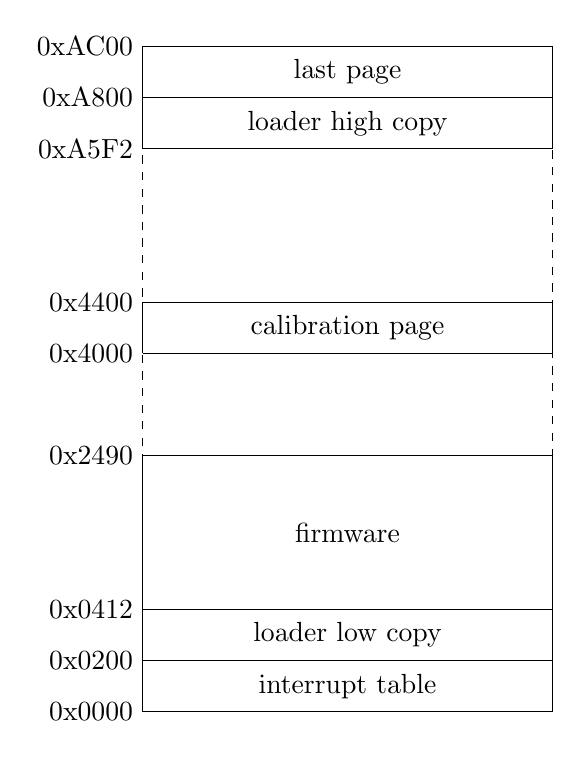
\begin{tikzpicture}[scale=1.3]
    \draw[dashed] (0,0) rectangle (4.0,6.5);
    \draw (0,0) -- (0,2.5);
    \draw (4.0,0) -- (4.0,2.5);
    \draw (0,3.5) -- (0,4.0);
    \draw (4.0,3.5) -- (4.0,4.0);
    \draw (0,5.5) -- (0,6.5);
    \draw (4.0,5.5) -- (4.0,6.5);
    \foreach \x/\y in {0x0000/0,0x0200/0.5,0x0412/1.0,0x2490/2.5,0x4000/3.5,
        0x4400/4.0,0xA5F2/5.5,0xA800/6.0,0xAC00/6.5} {
      \draw (0,\y) -- (4.0,\y);
      \node[anchor=east] at (0,\y) {\x};
    }
    \node at (2.0,0.25) {interrupt table};
    \node at (2.0,0.75) {loader low copy};
    \node at (2.0,1.75) {firmware};
    \node at (2.0,3.75) {calibration page};
    \node at (2.0,5.75) {loader high copy};
    \node at (2.0,6.25) {last page};
  \end{tikzpicture}\par}
  \caption{Program memory map (typical; exact addresses will vary; not to
    scale).}\label{fig:memory-map}
\end{figure}

The low copy runs first.  It is expected to write whatever parts of the new
firmware go into the top half of program memory -- including the new
firmware's high copy of the loader code.  The new loader code could
concievably differ from the old firmware's loader code, although new
firmware needs to be aware of any potential compatibility issues here.  Then
after the top half of the program memory space has been written, the new
firmware image directs the old loader, low copy, to jump to the newly
written high copy of the new loader.  That loader code continues the
operation of rewriting the program memory, filling in whatever parts of the
new firmware go into the low half of the
space.  At the end of the process, the entire rewritable portion of program
memory has, at least potentially, been rewritten.  All parts of the old
firmware, including the loader but excluding the non-reprogrammable last
page, can be replaced by the new firmware, despite the new firmware possibly
being the entire size of program memory.

I designed this process based on the observation that Microchip's C code
required something like 50K of program memory space just for a minimal USB
and FAT driver.  I expected that I could shrink the USB and FAT code
somewhat by replacing it with hand-optimized assembly language, but that I
would also have to add a significant amount of code to implement all the
rest of the things the firmware does beyond just reading files from a USB
mass storage device; so I could not be confident of making the entire
firmware \emph{less than half} the 64K capacity of the microcontroller. 
Being unable to fit two copies of the firmware in program memory at once was
the impetus for adding the SRAM chip.

In the event, my efforts to keep the code small were much more successful
than expected.  As of this writing the basically complete firmware fills
only about 17K of program memory, significantly less than half the available
space.  In principle, a scheme that read the entire new firmware into unused
space in program memory and then went from there, without needing the SRAM
chip, would probably work, and would save the cost of the additional
hardware.  However, the SRAM chip scheme is already implemented and it
works.  Writing and debugging a completely different loader system (as well
as changing the hardware design, even if only so far as just deciding not to
install the SRAM chip on the existing circuit board layout) seems like it
would be wasted effort; having the SRAM chip available for other purposes
seems to be of some value; and allowing for possible future firmware to use
all of program memory even if the current version uses less than half, seems
valuable too.  My plan is to stick with this design even if it seems
over-engineered for the current version of the standard firmware.

\section{Double assembly}

In order to help make sure that the low and high copies of the loader
function identically, they are both assembled from the same source file. 
Rules in the Makefile assemble the two object files loader-lo.o and
loader-hi.o from loader.s.  The symbol loader\_high\_copy is defined to 1 by
an assembler command-line option when assembling loader-hi.o, for use by
conditional assembly directives inside the source file in places where the
two copies need to differ.

The high copy should be located such that its text section (the binary
instructions that are the main output of the assembler) \emph{ends} with the
instruction at 0xA7FE, which is the last instruction before the reserved
final page of program memory.  The toolchain supports forcing a section to
start at a given address, but not easily forcing a section to end at a given
address.  (It might be possible with some trickery in the linker script, but
at the time I implemented this part, I was trying to avoid using a custom
linker script.) So in order to make the high copy end immediately before the
final page, more code in the Makefile reads loader-lo.o, finds the length of
the text section, and uses a Perl script named mkloaddr to write
loader-addr.inc, which contains the .section directive that will be used for
assembling the high copy to put it in the right place.

The mkloaddr utility finds the difference between the addresses marked by
the labels loader\_start and loader\_end in loader-lo.o.  It also applies an
adjustment defined by the loader\_delta label, if any.  This label can be
defined in the source code if there are any small differences between the
two versions of the loader that could affect the length.  It is measured in
address units, two units per 24-bit instruction, and it should be positive
if the high copy is longer, negative if the high copy is shorter.

Having two object files built from the same source unfortunately confuses
Microchip's debugger and I don't have a good solution to that, but it seems
to work reasonably well as long as execution stays in the low copy, and most
debugging tasks can be accomplished using only the low copy.

\section{Format of the image file}

Firmware to be loaded by the module needs to be formatted into an
\emph{image file}, so called because it is an exact image of the SRAM
contents at the start of the program memory writing process.  The standard
name for the firmware image file is firmware.frm (FIRMWARE.FRM in the
convention of the DOS FAT filesystem, which is case-insensitive but usually
writes filenames in all caps).  The image file can be up to 128K, the size
of the SRAM, though because there is only about 64K of program memory, it is
unlikely that an image file much larger than 64K would be useful.

The first 256 (0x0100) bytes of the image file are not used by the loader,
but are normally expected to be included in CRC checks.  This would be a
good place to include a human-readable identification of what the file is, a
copyright notice, and so on.

Starting at offset 0x0100, the main body of the file consists of a linked
list of \emph{loader records}, which are commands to the loader.  The loader
starts with the record at 0x0100 and then follows the links, executing each
command until one causes it to stop.

The first four bytes of each record are an identifier of the record type
(one byte, always an ASCII uppercase alphabetic character), and then a
24-bit pointer to the next record, as offset from the start of the file. 
Record types are referred to by their identifying letter, like
\emph{B-records} and \emph{C-records}.  After that header shared by all
record types, there may be other fields defined by the particular record
type, as discussed below.  Note that the next-record pointer is stored
\emph{unaligned} and \emph{little endian}; and the high byte of the pointer
is expected to always be equal to 0 or 1 because anything else would point
outside the 128K SRAM address space.  Notwithstanding the exception of the
24-bit next-record pointer, other fields in loader records of 16 bits or
more, and the records themselves, are expected to be 16-bit aligned.

Extra bytes of padding between and after loader records is allowed, a
fact used in the standard firmware's image generator to get around
toolchain limitations, as discussed in the section on image.s below.  In
principle, loader records need not even be arranged in sequential order
within the file; the loader just follows the link fields to successive
records wherever they are.

\section{SRAM simulation and common macros}

Debugging the loader works well on real hardware with a real SRAM chip; the
SRAM is tolerant of long gaps in the timing, as might be caused by
single-stepping the processor.  Debugging the loader code in the PIC24F
simulator works less well because there is nothing connected to the
simulated SPI port; the firmware tries to send commands to the SRAM chip but
never gets any responses.  So to allow for debugging in the simulator, there
is support in loader.s for building a small image file into program memory
and reading that instead of the SRAM.  If SIMULATE\_SRAM is defined in
config.inc, the loader will read SRAM data from program memory instead of
attempting to connect to the SRAM chip.

All communication with the SRAM in loader.s is done through seven macros:
assert\_cs2, retract\_cs2, mov\_to\_spi1buf, clr\_spi1buf, setm\_spi1buf,
mov\_b\_from\_spi1buf, and btst\_srxmpt.  When simulation is \emph{not}
enabled, each of these is defined to assemble a single instruction that
interacts with a relevant hardware register.  When SIMULATE\_SRAM is
defined, they instead implement a minimal simulation of the SRAM chip's
communication protocol, supporting only the read command.  There are a
couple of static variables and support subroutines assembled and used by
these macros.

The data stored in the the simulated SRAM is a manually-constructed image
file assembled at the label sram\_data.  It can of course be edited as
needed for a given debugging task, but the version in the source code is an
assortment of records intended to test all the major features of the loader.

\section{Loader initialization and main loop}

The initialization code at LOADER\_INIT, and its support routine
config\_timers\_for\_tunes, are not actually part of the loader proper; they
do not need to be duplicated and so are only assembled when assembling the
low copy, into the general-purpose .text section (to be located anywhere in
program memory) instead of into the loader\_lo section that gets located
immediately after the interrupt table, at address 0x0200.

The initialization sets up the hardware registers to both enable PSV for
reading the hardware ID from the final page, and have table read and write
instructions look at the first 64K of program memory (which is all of
program memory, anyway).  Then it calls config\_timers\_for\_tunes, which
configures Timers~1 and~3 and output compare~1 to the settings used by the
loader (mostly for playing the success and failure tunes, hence the name of
the subroutine), as well as PPS-mapping the output compare to both digital
output jacks.  This configuration is summarized in Table~\ref{tab:timers} on
page~\pageref{tab:timers}.  The config\_timers\_for\_tunes routine also
turns off all interrupts that can be turned off, by hacking the processor's
SR register to raise the processor interrupt level to~7.

Next, the initialization code turns off the front-panel LEDs by setting
TRISB bits~7 and~9.  It sends a RSTIO (reset I/O) transaction to the SRAM
chip.  This transaction makes sure the SRAM chip is configured for the
standard one-data-line SPI protocol, which is the default anyway, but it is
a safety measure in case the chip somehow got configured for one of the
other modes (which our hardware cannot support).  As usual with the SPI
hardware, each byte written must be matched by a byte read, in this case
done by a call to spi1\_read\_byte with the result discarded.

Next it initializes the starting address in the image, which is kept as 32
bits in the register pair W3:W2.  It sends a WRMR (write mode register)
transaction to the SRAM chip to set it to sequential mode.  Then it branches
to LOADER\_LO\_ENTRY, which is the start of the loader proper, at address
0x0200.  This is the start of the main loop of the loader; it expects that
all relevant initialization is already done and the current SRAM offset is
in W3:W2.

The main loop starts (at what is forced to be address 0x0200) with a
\insn{clrwdt} instruction.  Explicitly clearing the watchdog timer is rare
in the firmware because \insn{pwrsav} instructions occur frequently to wait
for interrupts, and have the side effect of clearing the WDT; but because
the loader runs with interrupts turned off, it needs to clear the WDT
explicitly at least once per second to avoid a timeout, and once per
iteration of the main loop is more than enough.

Next, it starts a sequential READ transaction with the SRAM, starting with
the first byte of the record, which is the record type identifier and gets
stored in the low byte of W1.  The next three bytes are the 24-bit address
of the next record; these get read into W3:W2.  The code requests another
byte after reading each one, and then requests one further byte without
reading it; so that after this point there are two bytes still expected from
the SPI port.  Subsequent code that handles the different record types
always either reads at least two more bytes (in which case it can be saved
the trouble of requesting two of them), or ends up resetting the module and
doesn't care about the state of the SPI bus.

The register W4 is initialized with the address of the start of the
\emph{common data} area for the convenience of the code sections that handle
the different types; most of these will end up reading the remainder of the
loader record directly into the start of the common area.

Then there are several sections that handle the different record types. 
Each section checks whether the already-read type identifier in W1 matches,
and branches to the next if it does not.  The last one, for F-records,
actually handles all cases not covered by the previous sections.

\section{B-record: burn a page}

The B-record tells the loader to burn (that is, erase and rewrite) a page of
flash program memory.  It is 1546 bytes long, with this layout.

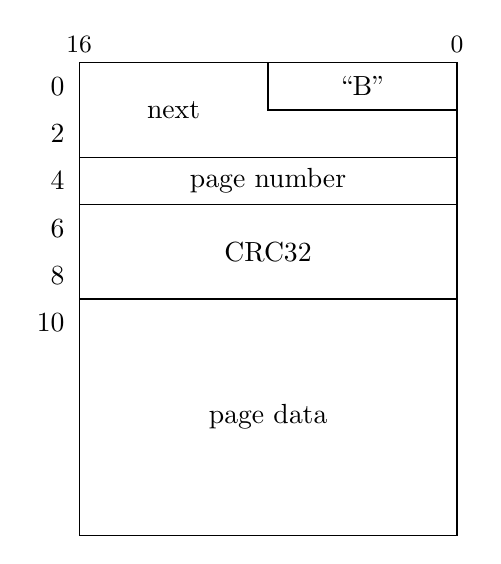
\begin{tikzpicture}[scale=0.3]
  \draw (0,0) rectangle (16,-20);
  \draw (8,0) -- (8,-2) -- (16,-2);
  \draw (0,-4) -- (16,-4);
  \draw (0,-6) -- (16,-6);
  \draw (0,-10) -- (16,-10);
%
  \node[anchor=east] at (-0.2,-1) {0};
  \node[anchor=east] at (-0.2,-3) {2};
  \node[anchor=east] at (-0.2,-5) {4};
  \node[anchor=east] at (-0.2,-7) {6};
  \node[anchor=east] at (-0.2,-9) {8};
  \node[anchor=east] at (-0.2,-11) {10};
  \node[anchor=south] at (0,0) {\small 16};
  \node[anchor=south] at (16,0) {\small 0};
%
  \node at (12,-1) {``B''};
  \node at (4,-2) {next};
  \node at (8,-5) {page number};
  \node at (8,-8) {CRC32};
  \node at (8,-15) {page data};
\end{tikzpicture}

The fields are defined as follows.

\begin{description}
  \item[``B''] Record type ID; ASCII character ``B,'' equal to 0x42.
  \item[next] Address of the next record, 24-bit little endian.  Lowest bit
    always zero because of word alignment, and upper seven bits always zero
    because of the 128K size of the SRAM.
  \item[page number] Page number to write.  This is technically the high
    byte of the program memory address for the start of the page, which must
    be aligned on a boundary of 1024 address units or 1536 bytes.  So the
    upper eight bits and the lower two bits of the 16-bit value in this
    field, are necessarily zero.  For example, to write the page starting at
    0x1400, the page number field contains 0x0014.
  \item[CRC32] The CRC32 value (parameters as used by Ethernet, ZModem, and
    so on) of the page data.
  \item[page data] The 1536 bytes that should be written to the specified
    page.
\end{description}

The code to handle this record type starts by calling
spi1\_finish\_transaction, a support routine that receives the bytes of the
record through SPI that were not already read by the main loop, and stores
them into the common data area.  Earlier in the source code, in the section
labelled ``Data memory,'' there were labels b\_record\_page, b\_record\_crc,
and b\_record\_data defined to ease access to the different fields in this
record.

Next, it checks the CRC32.  It calls the support routine start\_crc to
initialize the hardware, then runs a loop to call crc\_w0\_word for each
word of the page data.  Finally, it calls check\_crc\_result to verify that
the value in the record matches what the CRC32 hardware calculated.  Getting
good results from the CRC32 hardware is a little tricky, but the details of
that are encapsulated in the support routines.  If the CRC32 does not match,
then check\_crc\_result does not return; instead, it jumps to the failure
display, ending the loading process.

It is preferable to avoid any unnecessary writes to the flash program
memory, both to reduce wear and because writes take a relatively long time,
which is better to avoid for speed reasons.  So there is a further check to
see whether the data that would be written happens to match what is already
there.  This might be a common occurrence if someone tries ``updating'' a
module with the same firmware it already contains, or with a version close
to the existing one that may happen to contain identical bytes in some
places.  The loop starting at brec\_compare\_loop checks each byte of the
destination page in program memory against the proposed new data in RAM.  If
it detects no differences, then this is not an error, but the write for this
page should not proceed; in such a case the code just jumps back to
loader\_entry to read the next loader record, skipping further processing on
the current one.

If at least one byte does differ between the existing program memory and the
new data, then it will be necessary to erase and rewrite the page.  The code
sets up the flash SFRs for a page erase and calls perform\_flash\_operation
to pull the trigger.  Then it does the write, which is conducted one row (of
64 instructions, making eight rows in the page) at a time.  For each row, it
checks whether the entire row consists of instructions with the value
0xFFFFFF, which is the value that results from an erase operation.  If a row
of all 0xFFFFFF instructions is detected, then programming that row is
skipped (again, to reduce unecessary writes).

Once all eight rows have been checked and possibly rewritten, the code jumps
back to loader\_entry to handle the next loader record.

\section{C-record: do a CRC check}

The C-record requests a CRC check of a range of addresses in the SRAM.  It
is 16 bytes long, laid out like this.

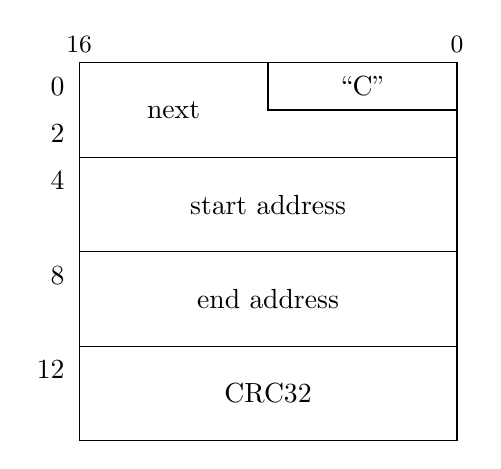
\begin{tikzpicture}[scale=0.3]
  \draw (0,0) rectangle (16,-16);
  \draw (8,0) -- (8,-2) -- (16,-2);
  \draw (0,-4) -- (16,-4);
  \draw (0,-8) -- (16,-8);
  \draw (0,-12) -- (16,-12);
%
  \node[anchor=east] at (-0.2,-1) {0};
  \node[anchor=east] at (-0.2,-3) {2};
  \node[anchor=east] at (-0.2,-5) {4};
  \node[anchor=east] at (-0.2,-9) {8};
  \node[anchor=east] at (-0.2,-13) {12};
  \node[anchor=south] at (0,0) {\small 16};
  \node[anchor=south] at (16,0) {\small 0};
%
  \node at (12,-1) {``C''};
  \node at (4,-2) {next};
  \node at (8,-6) {start address};
  \node at (8,-10) {end address};
  \node at (8,-14) {CRC32};
\end{tikzpicture}

The fields are defined as follows.

\begin{description}
  \item[``C''] Record type ID; ASCII character ``C,'' equal to 0x43.
  \item[next] Address of the next record, 24-bit little endian.  Lowest bit
    always zero because of word alignment, and upper 15 bits always zero
    because of the 128K size of the SRAM.
  \item[start address] Starting address of the range to check; 17-bit byte
    address stored as a 32-bit little endian unsigned integer, so the top 15
    bits are expected to be zero.
  \item[end address] Address of the first byte \emph{after} the range to
    be checked, as a 32-bit little endian unsigned integer; in consequence
    of that definition, end address minus start address equals number of
    bytes to check.
  \item[CRC32] The CRC32 value (parameters as used by Ethernet, ZModem, and
    so on) expected for the byte range.
\end{description}

The code for this record type starts by calling spi1\_finish\_transaction to
read the remaining 12 bytes of the record into the common data area.  Then,
it initializes the CRC32 hardware with a call to start\_crc, and starts a
READ transaction with the SRAM chip for the starting address of the range to
check.  It does a double-precision subtraction to find the byte count, and
runs a loop that reads that many bytes from the SPI port, sending each one
to the CRC32 hardware.  Finally, it calls check\_crc\_result to verify that
the value calculated by the hardware matches the one stored in the C-record. 
If the match fails, check\_crc\_result never returns; if it succeeds, the
C-record code ends with a branch to loader\_entry to handle the next loader
record.

Be aware that although a C-record can refer to any addresses in the SRAM, it
may be difficult or impossible to construct one that will succeed when the
range to be checked covers, overlaps, or contains bytes that depend on the
C-record's own CRC32 field.  Because of that and the fact that the range
must be a single interval, getting full coverage of the image file is a bit
tricky and requires multiple C-records.  See the discussion of image.s below
for how full coverage is achieved in the standard build.

\section{I-record: check hardware ID}

The I-record is intended to help make sure that a firmware image in this or
a similar format is really intended to be loaded on the hardware currently
trying to load it.  If at some point North Coast Synthesis were to release
other digital modules with a similar design, or if someone modified the
Gracious Host hardware in a way that would break the compatibility of
firmware images, then it would be important not to accidentally load a
firmware image intended for one of the hardware designs, on the other
hardware.  So to prevent problems in such a case, the hardware has a 64-bit
ID code, stored at the label HARDWARE\_ID at address 0xA800, in the first
eight bytes of the non-reprogrammable final page of program memory.  The
I-record specifies the intended hardware ID for the current image, and the
loader will abort if it sees an I-record that does not match the ID
of the current hardware platform.

The hardware ID for the Gracious Host, in the version described by this
manual (which as of this writing is the only version that exists), is 0x4D
0x53 0x4B 0x20 0x30 0x31 0x34 0x01.  That is the ASCII string ``MSK 014''
followed by a byte of value 0x01 which can be thought of as a version
number.

Please use a different hardware ID for any hardware that uses substantially
this image file format but is not 100\%\ compatible with firmware written
for the standard Gracious Host hardware.

The record layout is straightforward, just the common header shared by all
loader records, followed by the desired hardware ID.

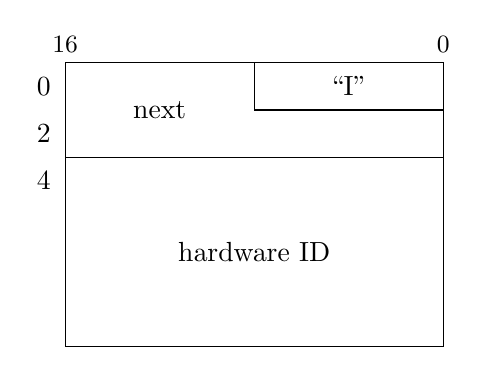
\begin{tikzpicture}[scale=0.3]
  \draw (0,0) rectangle (16,-12);
  \draw (8,0) -- (8,-2) -- (16,-2);
  \draw (0,-4) -- (16,-4);
%
  \node[anchor=east] at (-0.2,-1) {0};
  \node[anchor=east] at (-0.2,-3) {2};
  \node[anchor=east] at (-0.2,-5) {4};
  \node[anchor=south] at (0,0) {\small 16};
  \node[anchor=south] at (16,0) {\small 0};
%
  \node at (12,-1) {``I''};
  \node at (4,-2) {next};
  \node at (8,-8) {hardware ID};
\end{tikzpicture}

The fields are defined as follows.

\begin{description}
  \item[``I''] Record type ID; ASCII character ``I,'' equal to 0x49.
  \item[next] Address of the next record, 24-bit little endian.  Lowest bit
    always zero because of word alignment, and upper 15 bits always zero
    because of the 128K size of the SRAM.
  \item[hardware ID] The hardware ID to match against.
\end{description}

The code for this record type just loads the hardware ID from SRAM with a
call to spi1\_finish\_transaction, compares it against the one on the final
page of program memory, and branches to failure\_tune or loader\_entry
depending on the result of the comparison.

\section{J-record: jump to address}

The J-record tells the loader to jump (with a computed \insn{goto}
instruction) to a specified address in program memory.  This facility is
used midway through the loading process, after burning the high copy of the
loader, to transfer control to the new firmware's loader code instead of
depending on the low copy left behind by the old firmware.  It is also used,
at least in a standard firmware build, to start the calibration process
after loading is complete.

The record layout consists of the standard header, followed by the address
for the jump.

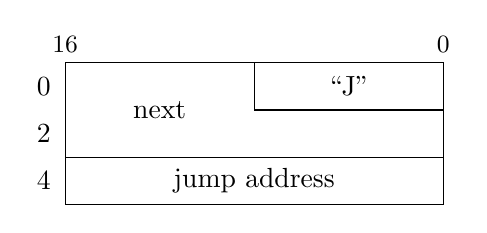
\begin{tikzpicture}[scale=0.3]
  \draw (0,0) rectangle (16,-6);
  \draw (8,0) -- (8,-2) -- (16,-2);
  \draw (0,-4) -- (16,-4);
%
  \node[anchor=east] at (-0.2,-1) {0};
  \node[anchor=east] at (-0.2,-3) {2};
  \node[anchor=east] at (-0.2,-5) {4};
  \node[anchor=south] at (0,0) {\small 16};
  \node[anchor=south] at (16,0) {\small 0};
%
  \node at (12,-1) {``J''};
  \node at (4,-2) {next};
  \node at (8,-5) {jump address};
\end{tikzpicture}

The fields are defined as follows.

\begin{description}
  \item[``J''] Record type ID; ASCII character ``J,'' equal to 0x4A.
  \item[next] Address of the next record, 24-bit little endian.  Lowest bit
    always zero because of word alignment, and upper 15 bits always zero
    because of the 128K size of the SRAM.  This is only used if loading
    continues after the jump; depending on where the jump is to, there may
    be no return from it.
  \item[jump address] Program memory address for the jump destination;
    16-bit little endian.
\end{description}

The code for this record just calls spi1\_read\_byte twice to get the jump
address, retracts CS2 to end the SPI transaction, and does the jump.

\section{S-record: succeed}

The S-record terminates the loader with a successful result.  As of this
writing, the standard firmware image does not actually use an S-record;
instead, when loading completes, it jumps to the calibration routine with a
J-record.  The image file contains an S-record at the end just in case
something causes the J-record to be skipped.  Successful calibration ends
with a jump to the global entry point SUCCESS\_TUNE, which calls
config\_timers\_for\_tunes and then branches into the S-record code, so this
code does in fact run after successful loading even though not invoked
through an S-record.

The only critical part of the S-record is the ``S'' at the start.

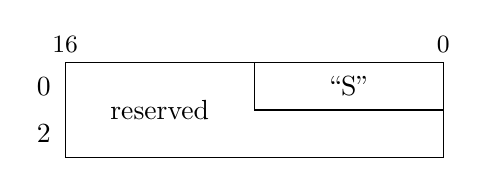
\begin{tikzpicture}[scale=0.3]
  \draw (0,0) rectangle (16,-4);
  \draw (8,0) -- (8,-2) -- (16,-2);
%
  \node[anchor=east] at (-0.2,-1) {0};
  \node[anchor=east] at (-0.2,-3) {2};
  \node[anchor=south] at (0,0) {\small 16};
  \node[anchor=south] at (16,0) {\small 0};
%
  \node at (12,-1) {``S''};
  \node at (4,-2) {reserved};
\end{tikzpicture}

The fields are defined as follows.

\begin{description}
  \item[``S''] Record type ID; ASCII character ``S,'' equal to 0x53.
  \item[reserved]  Although the S-record formally includes three bytes for
    the next-record pointer, these bytes are not actually used because
    executing an S-record terminates the loader.
\end{description}

The S-record code, starting from the label success\_tune, turns on the
front-panel LEDs and then runs 30 loops of playing a six-note tune that
takes two seconds to play, in square waves on the digital output jacks.  The
config\_timers\_for\_tunes subroutine will previously have set up output
compare peripheral number~1 (OC1) to be connected to those jacks and ready
to generate audio frequencies.

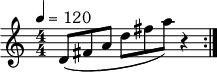
\includegraphics{success.cropped.eps}

Timing for the success display works using Timer~1, which has previously
been configured to 1:256 prescaler mode, 16\,$\mu$s per count.  At the start
of the loop the current value of the timer (TMR1 register) is captured into
W4.  Then at each step (for each note and the rest or pause at the end) code
in the support routine wait\_ticks computes a new target value for Timer~1
by adding an appropriate number to W4, and runs a tight loop that compares
TMR1 against the target value, terminating when they match exactly.  This
way there is no need for special handling of the timer overflow.  The loop
runs much faster than the 16\,$\mu$s counting rate of Timer~1, so it should
be unable to miss the exact match, especially bearing in mind that all
interrupts are turned off at this point.

In the success\_tune loop there are six calls to the support routine
play\_note, which sets OC1 to the period specified in W2 and then falls
through into wait\_ticks to wait 250\,ms, the duration of each note.  Then
the loop clears OC1R and OC1RS to make the output compare peripheral go
silent, and calls wait\_ticks with an argument value that makes it wait
500\,ms, for the rest at the end of the tune.

After 30 loops of the success tune, a \insn{reset} instruction reboots the
module.

Maintenance code 4935 invokes the success display.  See the discussion of
maintenance codes in the typing-keyboard driver documentation.

\section{F-record: fail}

The F-record terminates the loader with an \emph{unsuccessful} result; it is
basically similar to the S-record, but with a different display intended to
convey the idea of a failed loading attempt.  As with the S-record, current
firmware images never actually include F-records directly, but this record
type exists for testing, possible future use, as a destination for other
code paths that need to report failures, and to make it likely that files
other than valid firmware images will terminate processing quickly and
harmlessly.

In principle, the F-record's corrent type ID is ASCII ``F,'' but any loader
record with a type ID not otherwise handled will be treated as an F-record.

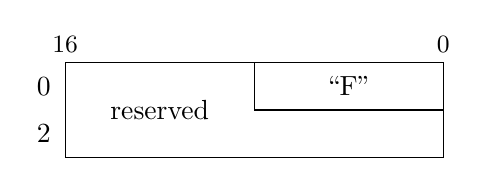
\begin{tikzpicture}[scale=0.3]
  \draw (0,0) rectangle (16,-4);
  \draw (8,0) -- (8,-2) -- (16,-2);
%
  \node[anchor=east] at (-0.2,-1) {0};
  \node[anchor=east] at (-0.2,-3) {2};
  \node[anchor=south] at (0,0) {\small 16};
  \node[anchor=south] at (16,0) {\small 0};
%
  \node at (12,-1) {``F''};
  \node at (4,-2) {reserved};
\end{tikzpicture}

The fields are defined as follows.

\begin{description}
  \item[``F''] Record type ID.  ASCII character ``F,'' equal to 0x46, is
    guaranteed to be treated as an F-record, but any value that is not the
    ID of some other record type will be treated as an F-record by default.
  \item[reserved]  Although the F-record formally includes three bytes for
    the next-record pointer, these bytes are not actually used because
    executing an F-record terminates the loader.
\end{description}

The code to handle F-records, starting from failure\_tune, is similar to
that for the success tune, but a little simpler because there are only four
notes, no rest, and the frequencies alternate between low B and other
pitches.

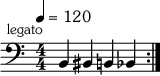
\includegraphics{failure.cropped.eps}

The play\_failure\_notes support routine plays two notes of 500\,ms each,
one low B and one other pitch specified by the period in W2, with the LEDs
turned off for the first note and on for the second.  The failure tune loop
is basically just two calls to play\_failure\_notes.  Before the loop, it
sets the colour of the front-panel LEDs to red.  After the loop, it executes
a \insn{reset} instruction to reboot the module.

The (capitalized) FAILURE\_TUNE global symbol is available for other code
paths to play the failure tune.  It just calls config\_timers\_for\_tunes to
set up the hardware and falls through into (uncapitalized, non-global)
failure\_tune.  FAILURE\_TUNE is conditionally assembled only in the low
copy of the loader, and its absence from the high copy is counted in
loader\_delta.

Maintenance code 6697 invokes the failure display.  See the discussion of
maintenance codes in the typing-keyboard driver documentation.

\section{Support routines}

The loader source file ends with a few support routines used by the code
above.  Several of these are also exposed as global symbols, only in the low
copy according to conditional assembly directives, because they are useful
elsewhere in the firmware.

The spi1\_read\_byte routine (also SPI1\_READ\_BYTE, used in the USB Mass
Storage driver) reads one byte from the SPI bus, either because we actually
want to read a byte, or to keep up the read/write balance needed to make
written bytes pass through the system.  The new byte goes into the low byte
of W0, and the previous low byte of W0 is swapped into the high byte, which
is useful when reading a 16-bit number with two successive byte reads.

The spi1\_finish\_transaction routine is specific to the loader and not
globally exposed.  It takes a byte count in W5 and reads that many bytes
from SPI into data memory starting at the address in W4, with the assumption
that exactly two of those bytes have already been requested (so it makes
W5$-$2 requests for new bytes).  It also closes the SPI transaction assumed to
already be in progress.  Some per-record-type handlers use this to load the
rest of their record data after the header.

The success and failure tunes use play\_failure\_notes, play\_note, and
wait\_ticks, each already described.

Then there are several routines for dealing with the CRC hardware.  The
start\_crc routine (globally exposed as START\_CRC) sets up the SFRs for the
CRC32 peripheral to start a CRC calculation, telling it to use 8-bit data
transfers and a 32-bit polynomial size.  The polynomial, in the format
required, is set by the constant crc\_polynomial and equal to
$x^{32}+x^{26}+x^{23}+x^{22}+x^{16}+x^{12}+x^{11}+x^{10}+x^8+x^7+x^5+x^4+x^2+x+1$
(hex value 0x04C11DB7, with the 33rd bit omitted).  This code also sets the
peripheral's shift register value to the constant crc\_init, which is
0x46AF6449, the value needed to make the PIC24F's CRC32 peripheral match the
behaviour of the CRC32 algorithm which specifies 0xFFFFFFFF initialization.

I think, though this initialization value came mostly from trial and error
in the simulator rather than a deep understanding of how the hardware works,
that what is going on here is that 0x46AF6449 is the value that would end up
in the register if we started with zero and then hashed 0xFFFFFFFF on the
data input, which is equivalent to what the standard's somewhat different
representation would call starting with 0xFFFFFFFF in the first place.  This
surmise is supported by other tricky distinctions in the handling of the
final check at the end.  It appears that the PIC24F hardware may be in some
way inside-out relative to other descriptions of CRC32.  I was not able to
find good example code for this hardware that I could adapt for my purposes;
common wisdom among PIC24 programmers seems to be that the CRC32 peripheral
is just too complicated, and it is better to implement the algorithm in
software.

Proceeding with the hardware-based implementation, the crc\_w0\_word routine
(exposed globally as CRC\_W0\_WORD) accumulates a 16-bit value from W0,
\emph{little endian}, into the ongoing calculation by loading its two bytes
into the hardware FIFO and falling through into run\_crc.  That routine
(exposed globally as RUN\_CRC) triggers the hardware to start processing
bytes from the FIFO and then waits for it to empty the the FIFO.  Note that
the CRC32 hardware processes only one bit of input at a time, but runs at a
clock speed of twice the processor clock (therefore, 32\,MHz); so it runs
one byte per four instructions and the wait is unlikely to be significant. 
Although in principle the hardware is designed to allow the CRC32 to crunch
away while the processor is doing something else, adding buffer fill
juggling on top of the other complexities of using this hardware seems
unlikely to be worthwhile.

The final support routine for CRC calculation is check\_crc\_result.  It
works by running four data bytes from the address specified in W1 into the
CRC32 hardware as if they were additional data bytes, and then checking
whether the shift register contains 0xFFFFFFFF.  If the four bytes from [W1]
were the correct CRC32 value of the data processed before this point, then
the shift register should indeed end up containing 0xFFFFFFFF, indicating a
correct match.  In that case, check\_crc\_result returns.  Otherwise, it
branches to failure\_tune.

The last support routine in the source file is perform\_flash\_operation,
exposed as a global symbol PERFORM\_FLASH\_OPERATION with the addition of a
\insn{disi} instruction to temporarily disable interrupts, which is
unnecessary in internal calls because the loader runs with interrupts
globally disabled.  Apart from that wrinkle, this code is as specified in
the microcontroller data sheet.  Its function is to commence primary
ignition on a flash program memory operation, the details of the operation
having been previously specified by writes to various SFRs and
flash-specific write latches.  Because doing such a thing is dangerous, the
hardware requires very specific steps with precise timing to ``arm'' and
trigger the operation; otherwise, the request will be ignored.  After
triggering the flash operation, the code contains a tight loop which waits
for the hardware to indicate the operation is complete.  The data sheet says
that an erase requires 40\,ms minimum, and a write requires 3\,ms typical,
though I could not find a timing diagram or a clear explanation of whether
that refers to a row or a single-instruction write, or whether those two
kinds of writes may have the same duration.

At the end of loader.s, the loader\_end label captures the assembly location
counter at the end of the double-assembled section, for use by mkloaddr to
calculate the location of the high copy.

\section{Image generation overview}

The source file image.s generates the loadable image, using the assembler to
piece together the records with the proper link addresses and so on.  The
basic concept was that using the same toolchain that generates ordinary
object files would make it easy to do things like make a J-record point at
the address of its target.  Unfortunately, bugs and limitations in the
assembler and linker mean that much of the logic for building the image ends
up implemented in macros instead of directly using the
assembler features, and there are several pieces of support code that need
to be invoked by the Makefile to get information into and out of the image
generator.  It is less simple than originally intended; but it does work.

One limitation in particular is that, because the image file gets assembled
into an object section of ``customized data memory'' type, it is not treated
as code by the toolchain, and some of the toolchain features that would be
available in code sections are unavailable.  (Trying to make it code instead
raised other problems and proved unworkable.) In particular, I was unable to
attach a label to a point in the image file and then say ``These bytes right
here should be filled in with the address of that label.'' Filling in such
bytes would normally be a function performed by the linker, and the linker
refuses to touch customized data memory.  So I ended up having to perform
the ``bytes should be the address of label'' operation by writing my own
code to extract the addresses of symbols and then fill them into the image,
defeating one of the original purposes of using the assembler for image
generation.

Another assembler limitation is that customized data memory spaces cannot be
bigger than 64K, and addresses within them cannot be bigger than 16 bits. 
The SRAM is 128K, requiring 17-bit addresses.  I dealt with that limitation
by actually defining two customized data memory spaces (referred to in the
source code as the low and high \emph{mobies}), with some logic required to
handle switching between them where necessary.  In practice, firmware is
unlikely to grow so big as to require the use of both; but in principle,
program memory is slightly greater than 64K all by itself (because of the
weirdness arising from its 24-bit width); firmware could fill all of program
memory; and the overhead of packaging it in loader records could push the
image file further past the moby boundary.

The Makefile builds the firmware binary by first running the assembler to
generate object files (*.o) from the assembly-language source files (*.s). 
In general there is one object file for each source file, although as
discussed above, loader.s actually builds two object files, loader-lo.o and
loader-hi.o.  Then the linker runs to decide the final addresses of all the
sections of code and combine the object files into a single unified binary
file (firmware.elf) that represents the entire contents of program memory. 
This file is in ELF format, the same format that under Linux (since version
1.2, anyway) would be an executable file.  For ICSP purposes, the ELF file
can be translated to a .hex file, which is the format usually used by
chip-programming hardware tools; the Makefile includes a rule to do that if
desired.

However, to generate a file that can be loaded by the module itself over the
USB port, there are more steps needed.  The Makefile uses the toolchain's
objdump utility, piped into a Perl script named dmp2bin, to generate the
files firmware.bin (which is a plain image of the contents of program
memory, all 66048 bytes of it) and fw-pages.inc, which defines symbols with
names like \_\_page\_exists\_\_00 for all the pages that contain data and
will need to be programmed.  These files are used as inputs by image.s to
decide which pages need B-records and to provide the data bytes for those
B-records.

Another Makefile rule generates the file firmware.syms from firmware.elf by
running the toolchain's nm utility.  This file lists all the program memory
addresses of symbols in the firmware.

Two more include files needed by image.s are image-syms.inc, which includes
the CRC values of parts of the image file for use in C-records, as well as
the addresses of symbols jumped to by J-records; and image-id.inc, which
includes metadata about the current build:  the username, hostname, and date
as reported by Linux command-line utilities.  Both of these files are
generated inside the final firmware.frm Makefile rule.

The rule that finally generates firmware.frm is a shell script written into
the Makefile, that puts together all the pieces.  One of the problems to be
solved is that the image file needs to contain CRC32 values for parts of
itself.  In order to calculate those values and write the image file, we
must already have the image file, creating a problem of where to start.  The
solution is that the Makefile rule is a shell-script loop: it builds the
image file using dummy data for the CRC32 values, then calculates new CRC32
values based on the result, and re-generates the file using those values. 
It repeats until the firmware.frm file does not change between two
iterations.  The CRC32 values do not (at least, should not) actually depend
upon \emph{themselves} directly or indirectly, only upon \emph{other bytes
in the file}, so the process terminates after two or three iterations.

In more detail, the Makefile rule initializes firmware.frm to a zero-length
file and image-syms.inc to a file containing a single newline.  (Use your
imagination for why the newline is necessary.) It creates the file
image-id.inc using the whoami, hostname, and date commands.  Then it
assembles image.s.  The macros in image.s figure out everything that should
be in the loadable image, but because image-syms.inc defines no symbols, the
macros just use dummy values for all the CRC32s and J-record destinations. 
After this assembly step, the Makefile rule does some bookkeeping for Make's
dependency tracking, uses nm to generate image.syms, and uses dmp2bin to
generate a tentative firmware.frm file.  This first version will not
actually be usable because of the dummy CRC32 and J-record data.

Then the loop starts.  It runs a Perl script called mkimagesyms, which
generates the image-syms.inc file based on the information in the tentative
firmware.frm, and the firmware.syms and image.syms files.  The script does
several things, controlled by symbols that were defined in image.s.

\begin{itemize}
  \item If symbols named like \_\_crc\_start\_\_XXXX and \_\_crc\_end\_\_XXXX
    are defined, then mkimagesyms will compute the CRC32 of the bytes between those
    symbols in firmware.frm, and will define a symbol in image-syms.inc named
    like \_\_crc\_\_XXXX and equal to the CRC32 value.
  \item When it computes a CRC32 value, mkimagesyms will also define
    symbols in image-syms.inc named like \_\_crc\_addra\_\_XXXX and
    \_\_crc\_addrz\_\_XXXX and equal to the starting and ending addresses of
    the CRC32 calculation.  These differ from 
    \_\_crc\_start\_\_XXXX and \_\_crc\_end\_\_XXXX, despite normally having
    the same numerical values, because these new symbols have the
    data type of plain numbers, not address labels.  The assembler can set
    data bytes equal to them, which it would refuse
    to do with address labels.  They also are adjusted by the
    \emph{moby} feature below to contain the 17th address bit that the
    assembler refuses to handle.
  \item If a symbol named like \_\_moby\_\_XXXX is defined, then the value
    of that symbol times 0x10000 (that is, 64K) is added to the address of
    the symbol \_\_XXXX before \_\_XXXX is used for other purposes. 
    This facility would normally be used for CRC32 start
    and end addresses, with symbols named like
    \_\_moby\_\_crc\_start\_\_XXXX, to express which half of the 128K SRAM
    actually contains a given address.
  \item If a symbol named like \_\_psym\_\_XXXX is defined, then mkimagesyms
    will define that symbol in image-syms.inc to have the value of the
    \emph{program memory} address of the symbol XXXX in the firmware, taken
    from firmware.syms.  This is used for J-record targets.
  \item It detects whether the image-syms.inc file it is writing is
    identical to the one that previously existed, and returns a success exit
    code (exit code zero) if so.
\end{itemize}

Then the script runs the assembler on image.s again.  The image.s file
includes image-syms.inc, which now gives real (though perhaps not final)
values to the CRC32 and J-record values.  The script runs the steps to
regenerate image.syms and firmware.frm, then repeats until mkimagesyms
returns exit code zero.  It displays the sha1sum output for
image-syms.inc on each iteration, to give the user some idea that progress
is being made, although the actual check for loop termination is on exact
equality, not on the sha1sum result.

\section{The image generator source file (image.s)}

The source file image.s puts the pieces together.  It starts by including
global.inc (like all the firmware source files); fw-pages.inc (which
contains a symbol per page identifying the pages to burn); and
image-syms.inc (generated by mkimagesyms, as above).

Then it sets up a memory space for each 64K moby of the SRAM (spaces named
\_sram\_lo and \_sram\_hi), defines max\_record to 1546 to represent the
largest possible loader record (which is needed for detecting when to switch
mobies).  It opens an assembly section in \_sram\_lo, which will be the
destination for the image data; then it starts defining the support macros.

The basic flow is that we keep a shadow location counter in the symbol
\_\_location, which records where we are currently assembling things into
the SRAM's space.  Keeping it in a symbol of our own is necessary because
the assembler narrowly limits the ways we can use the value of its own
location counter.  As we create loader records with the macros defined for
the purpose, this symbol gets updated to reflect where the next record will
be created.  When it is detected that the next record will not fit in the
current moby (or \emph{may} not fit -- the check is based on the assumption
of a maximum-length record), the macros automatically close the low moby
section and start assembling into a new section for the high moby.

The check\_moby macro comes first.  It just checks whether \_\_location plus
the maximum record size would exceed 64K, and if so, switches to a new
section.  This needs to be a separate macro because of an assembler bug:  if
we start a new section inside a macro and assemble bytes into that section
inside the same macro then the listing file is messed up.

So the loader\_record macro, which assembles the start of a loader record
(type ID and next-record link), is a separate macro, and the main source
code normally runs check\_moby before each invocation of loader\_record. 
The loader\_record macro takes as arguments the record type (one ASCII
character), a name used for defining a symbol associated with this record,
and the record's size in bytes.  The address of the next record is
calculated using this size, with appropriate adjustment for whether the next
record is being moved into the next moby.

The first 0x0100 bytes of the file contain an ASCII copyright notice and
version identifier.  The image-id.inc file gets included here so that the
firmware file will be automatically stamped with basic metadata.

Loader records start at address 0x0100.  The first is an I-record, requiring
the hardware ID to match the Gracious Host's.  Then come two C-records which
together cover the entire file.  There is a macro called store\_crc defined,
which takes a name like XXXX as an argument and checks whether the symbol
\_\_crc\_\_XXXX is defined.  If it is (because it came from image-syms.inc),
it assembles four bytes containing the symbol value.  If not, it defines the
symbol to the value 0xDEADBEEF, which will trigger mkimagesyms to generate a
proper value for it on the next iteration, and assembles bytes with that
value instead.  This macro is also used by the page-burning records later.

The two C-records interlock to cover the entire file.  The first one,
referred to as the ``hi'' C-record, covers everything after the CRC field of
the ``lo'' C-record, which is next.  The ``lo'' record covers everything
before its own CRC field, including the entirety of the ``hi'' record.  This
arrangment guarantees that every byte of the file either is covered by some
CRC, or is part of a CRC field, without any circular dependencies.  Any file
corruption in the class of errors detectable by the CRC32 algorithm will
result in at least one of these two checks failing.  For greater certainty,
the B-records also have CRC checks of their own.

The B-records are next.  There is a macro named burn\_page defined, whose
function is first to check whether a symbol named like
\_\_page\_exists\_\_00 has been defined.  If so, that indicates the
page in question needs to be included in the firmware image.  It sets up a
header for a B-record; calls store\_crc to either assemble the data bytes
for the CRC of the page (if they have been defined) or else assemble
0xDEADBEEF and define the symbols that request calculation of this CRC; and
then includes the appropriate 1536 bytes from firmware.bin with an
``.incbin'' directive.

The source file calls burn\_page for each page from 0xA4 down to 0x50 in
descending order, using the assembler's ``.irpc'' looping construct to
abbreviate the loop.  That will program roughly the top half of program
memory, for the pages actually defined in the firmware.  At this point
loader records are still being interpreted by the old firmware's low loader
copy.  But after page 0x50, there is a J-record pointing at
LOADER\_HI\_ENTRY, with the address for that retrieved by mkimagesyms
through the \_\_psym\_\_ feature.  This directs the old firmware's loader to
jump to the high copy of the new firmware's loader, which ought to have been
in the pages just burned.  Subsequent loader records are actually executed
by the new firmware's loader.

There follows another .irpc loop to burn all defined pages from 0x4C down to
0x00.  After that, firmware update will be complete.  The image file source
assembles another J-record to jump to CALIBRATION\_PROCEDURE, which should
terminate loader processing.  But it also assembles a final S-record as a
backstop.


% $Id: firmwares.tex 9772 2022-01-19 04:17:12Z mskala $

%
% Gracious Host firmware framework
% Copyright (C) 2022  Matthew Skala
%
% This program is free software: you can redistribute it and/or modify
% it under the terms of the GNU General Public License as published by
% the Free Software Foundation, version 3.
%
% This program is distributed in the hope that it will be useful,
% but WITHOUT ANY WARRANTY; without even the implied warranty of
% MERCHANTABILITY or FITNESS FOR A PARTICULAR PURPOSE.  See the
% GNU General Public License for more details.
%
% You should have received a copy of the GNU General Public License
% along with this program.  If not, see <http://www.gnu.org/licenses/>.
%
% Matthew Skala
% https://northcoastsynthesis.com/
% mskala@northcoastsynthesis.com
%

\chapter{Firmware framework (firmware.s)}

The firmware.s file contains what might be called the ``main program'' of
the firmware:  the code that runs at power-on reset, sets up the basic
configuration of the hardware, and then dispatches to
other modules.  It also contains some global infrastructure that simply
needed to be \emph{somewhere}, such as the declaration of the common data
area.

In this chapter I also describe the global include file, global.inc.

\section{Microcontroller configuration}

The configuration registers (``fuses'') and their values are declared at the
start of firmware.s, with some conditional assembly to take into account
configuration settings from config.inc.

At the bottom of this section there is also a quick declaration of the
common data area for use by the \insn{in\_common} macro.

\section{Last page}

The last 1.5K page of program memory cannot be reprogrammed (or,
technically, it cannot be safely \emph{erased}) by the microcontroller under
its own software control; only by in-circuit programming.  So this area can
only be used for data that is never expected to change.  In the Gracious
Host that is an eight-byte hardware identifier (ASCII ``MSK 014'' followed
by byte 0x01) at symbol HARDWARE\_ID, address 0xA800; followed by a table of
divisors at symbol NOTE\_TBL, address 0xA808.  The divisors are intended to
be used with output compare modules to provide musical-note frequencies. 
The firmware Makefile calls a Perl script to generate the file notetbl.inc,
which is imported to firmware.s by an include directive.

Later bytes of the last page, past the end of the note table, include a
human-readable copyright and version control ID; but be aware that if you
read these bytes out on a real-life module, they will represent what was
programmed into the chip the last time it underwent ICSP.  Firmware loaded
later by USB could have rewritten other parts of the program memory, so
might not be the same version identified by the notice on the last page.

\section{Power-on reset}

At reset the microcontroller starts executing code at symbol \_\_reset,
which begins by initializing the stack and the TBLPAG register.  If
FILL\_RAM\_DEAD is selected, it will fill all the general-purpose RAM with
the value 0xDEAD.  Then it opens a TRY/TRIED block with a handler that
points at a \insn{reset} instruction, just to catch stray THROWs executed by
other code, and calls STANDARD\_IO\_CONFIG (defined later this same file) to
set up most of the on-chip peripherals.

Next, the reset handler sets up PPS mappings for the SPI peripheral, and
calls CALIBRATION\_TO\_RAM from calibration.s to extract the curren DAC and
ADC calibration values.

Optionally, if requested by configuration symbols, it branches at this point
to RUN\_TESTS for tests from tests.s, or to \_USB\_MASS\_ENTRY to attempt
reading a simulated filesystem image.  Normal production firmware will
instead fall through into the non-USB behaviour.

\section{Non-USB behaviour}

This section of firmware.s contains the top-level loop that manages the
module's functions when there is no USB device inserted.  Before the loop it
calls USB\_INIT to set up the USB driver for detecting when a device is
inserted, sets up the PPS mapping to send output compare units 1 and 2 to
the left and right digital jacks, and does a couple of other small
initializations like setting the LED colour to red.

This code uses W8 for the current state of the envelope, encoded on a scale
where each count of the register value corresponds to $1/(12\times 256)$ of
a volt and 0x2400 is 0V.  That is the scale (MIDI note number in high byte,
fraction in low byte) used by the calibration API.

The non-USB behaviour (as described in the UBM) is a baby synthesizer voice:
V/oct pitch CV in on the left, gate CV in on the right, and quantized pitch,
envelope, and quantized and unquantized oscillator outputs.  While managing
these functions, the loop is also constantly looking for a USB device to be
inserted.  When one is, it branches off to the general USB driver to handle
the device.

The main loop starts by idling the microcontroller to wait for an interrupt,
which also refreshes the WDT.  It checks whether the USB driver has detected
a device attach, breaking out of the loop if so.  If the module booted up
with a device already attached, that fact will be detected as a device
attach on the first run through the loop.  Then if the loop did not break
for a device attach, it checks whether input 2 is high (gate CV high).

If the gate is low:  it turns off the LEDs and the unquantized oscillator
output, then conditionally on whether a 618\,$\mu$s tick has occurred (from
the ADC subsystem, used here for envelope timing) it updates the envelope
value -- release phase, ready for a new attack, with the envelope voltage
heading for zero.  After an envelope update it branches to
tune\_oscillators, the shared code for setting the oscillator frequencies.

If the gate is high: it turns on both LEDs, then similarly checks for a
618\,$\mu$s tick.  If there has been one since last update, it updates the
envelope, which is a little more complicated because it could be in the
attack, decay, or sustain phase.  Once the new envelope value is in W8, it
falls through to tune\_oscillators.

From the tune\_oscillators label, the code calls ADC1\_TO\_NOTENUM from
calibration.s to get the input voltage from the left channel, and then
CALC\_OSC\_TUNING (later in this same file, global because it may be useful
elsewhere) to find the output compate period value for the unquantized input
note using interpolation between values from NOTE\_TBL.  This is written into
output compare unit 1 conditionally on the gate input being high.

Then the note value, which is in W7, gets rounded to the nearest semitone by
adding 0x80 and zeroing the low byte.  That quantized value is sent to the
left DAC channel and looked up in NOTE\_TBL; no interpolation needed because
it is an exactly tuned note.  The resulting quantized period value is sent
to output compare unit 2, unconditionally.

Finally, the loop sends the current envelope value to DAC~2, and loops back
to wait for another interrupt.

The non-USB loop breaks out to non\_usb\_done when the USB driver tells it a
device has attached.  At that point it changes the LEDs to solid green,
turns off the output compare oscillators, sets up a TRY block with
catch\_usb\_session as the handler, and then calls USB\_HANDLE\_SESSION,
which in the ordinary course should do all the handling of enumerating and
configuring the device, choosing a driver, and running the device driver
until the device is removed.

In case of an exception thrown and not caught during the driver execution:
catch\_usb\_session sets up the LEDs to bring rapidly back and forth in
red, using calls to the LED blinker driver.  It waits for the USB driver to
report device detach, then falls through into the normal-case code run when
the USB driver returns without throwing.

Finally, there is a little bit of cleanup:  the top-level code calls
USB\_DONE and LEDBLINK\_DONE to clean up after the USB and LED blinker
subsystems, particularly by turning off relevant interrupts.  These calls
are harmless if the relevant drivers were in fact already shut down.  Then
it loops back up to the initialization before the main non-USB behaviour
loop.

CALC\_OSC\_TUNING is declared global in case it may be useful elsewhere.  It
calculates a period value to tune an output compare for a MIDI note, with
interpolation for fractional note numbers.  The input note number (high byte
is MIDI note, low byte is fraction) is expected in W0.  It copies that value
to W7, extracts the entries on either side of the fractional note from the
NOTE\_TBL structure, and then interpolates between them, using a tricky
\insn{mov.b}/\insn{swap} combination to divide the 24-bit intermediate value
by 256 in only two instructions.  The address of NOTE\_TBL is left in W6 as
a side effect.

\section{Basic I/O}

This file provides a few basic subroutines for I/O that it needs itself and
might be needed elswhere.  UNLOCK\_PPS does the necessary unlocking sequence
to allow changes to the PPS mapping registers; LOCK\_PPS, similarly, locks
them up again.  Note that there is no automatic handling of nesting for
these operations.  They just set the current state of the registers to
locked or unlocked, regardless of whether it duplicates the previous state,
and they trash W0, W3, and W4.

STANDARD\_IO\_CONFIG sets most of the on-chip peripherals to sane default
values.  It clears the soft interrupt flags (discussed below); sets the data
direction for the GPIO pins; and configures the interrupt priorities.  It
sets up Timers~1, 2, and~3 to their standard configurations, which are
intended to support LED blinking (Timers~1 and~2) and the ADC conversion
schedule (Timer~3).  It turns off Timers~4 and~5.

It sets up all the output
compare units to edge-aligned PWM mode, driven by the Timer~3 prescaler, but
with modulation values that will actually keep their outputs low all the
time.  It sets up the ADC subsystem to its standard configuration, scanning
the two analog input jacks and the USB bus voltage, one conversion per
Timer~3 reset, and one interrupt after each completed cycle of three
conversions (1.618\,kHz interrupt frequency).

Then it sets the comparators to look at the analog input jacks, with a
reference voltage equivalent to $+$1.62V at the jacks, and interrupts enabled
on rising edges through that voltage.  Note that in hardware testing, it was
apparent that interrupts are also sometimes generated on falling edges; this
is not a published erratum but may be related to one, and we work around it
in the ISR, which is in calibration.s.

Finally, STANDARD\_IO\_CONFIG sets up the SPI peripheral for talking to the
SRAM and DAC, and clears the soft interrupt flags a second time to deal
with any spurious interrupts that might have come in while the peripherals
were being reconfigured.

Two more global I/O routines set up PPS mappings used in firmware.s and
possibly of use elsewhere:  PPS\_MAP\_OC\_DOUT sets output compare units~1
and~2 to the two digital output jacks, and PPS\_MAP\_GPIO\_DOUT sets the
pins for these outputs back to plain GPIO mode.  Each of these routines
makes further calls to unlock, and then lock, the mapping registers around
its writes to the registers.

\section{A/D conversion and USB short detect}

The A/D conversion ISR is to some extent a safety feature, so it is expected
to be active pretty much all the time the module is powered up -- possibly
not during the special operations of calibration and firmware reloading.  It
extracts voltage measuerments from the ADC hardware buffer and writes them
to global variables.

Global variables defined here are SOFT\_INT\_FLAGS, INPUT\_ADC1, INPUT\_ADC2,
and USB\_VBUS\_ADC, each one word long.  The other three simply represent
raw ADC readings (10 bits each), updated by the ISR at 618\,$\mu$s
intervals, but SOFT\_INT\_FLAGS is used by several different subsystems that
need to wait for interrupts handled by specific ISRs; the ISR is expected to
set an appropriate bit in the variable, and then the foreground code can
check for that bit after coming out of idle to recognize when the desired
interrupt (as opposed to some other interrupt) has actually occurred. 
Constant values for bit numbers within this variable are defined by
symbols with names starting ``SI\_'' in global.inc.

As well as writing the current ADC readings to variables, the ADC ISR checks
whether the one for USB voltage is too low (indicating that a short circuit
or other problem has caused the polyfuse to trip) and sets the soft
interrupt flag SI\_VBUS\_TRIP, if the voltage is low and has been low
on more than 162 consecutive ADC interrupts, corresponding to 100\,ms.

Before returning, the ISR sets (unconditionally) the soft interrupt flags
for ADC1 and ADC2; separate flags because there could be two different
things in the foreground waiting for them, as for instance during
multi-threaded calibration.

The last thing in the firmware.s file is a subroutine called CHECK\_VBUS,
which is the consumer of the SI\_VBUS\_TRIP flag.  The foreground ought to
call this periodically when a USB device is attached, to shut down the
module in the event of trouble with the USB power.  It checks for whether
the ISR has set the flag, then if so, it shuts down the USB driver, PPS
maps the output jacks to plain GPIO, sets the LEDs to blink in a unique
red/green flicker pattern, and then waits, checking the bus voltage after
every interrupt, for the voltage to remain good for 1618 consecutive ADC
interrupts, corresponding to one second -- the pattern expected if the short
circuit is resolved and the polyfuse cools down.  Then it resets the module.

In practice, a power disruption serious enough to trip the polyfuse is
likely to also disrupt the microcontroller enough that it will be unable to
continue executing instructions until a power cycle, so the semi-graceful
reset contemplated by CHECK\_VBUS is mostly theoretical.  But this code
seems to give it the best chance of recovering under software control.  It
has to be called in the foreground (instead of the ISR just branching
directly into the recovery loop) because logic like the LED blinking also
uses interrupts and trying to keep all that running well without returning
from the ADC interrupt would be inconveniently complicated.

\section{Global include file}

Every .s file includes global.inc, which contains standardized definitions
used everywhere.  This file contains nested includes of Microchip's
p24Fxxxx.inc file, which defines things like register names, and config.inc,
which defines build-time options.  The build-time options are described in the
``Build environment and tools'' chapter of this manual.

These things are defined in global.inc:
\begin{itemize}
  \item the \insn{in\_common} macro for defining file-local static memory
    assignments in the common data area, with its support symbols;
  \item data structure sizes for the USB low-level support;
  \item BUFFER\_SAFETY\_MARGIN, the minimum number of extra bytes added to
    buffers to mitigate overruns by the USB hardware;
  \item STACK\_RESERVATION, the minimum amount of stack space that the mass
    storage buffer allocator will leave unconsumed;
  \item symbols starting SI\_ (``soft interrupt'') representing bit numbers
    in the SOFT\_INT\_FLAGS variable;
  \item symbols starting UF\_ (``USB flag'') representing bit numbers, and
    starting UFM\_ (``USB flag mask'') representing masks ($2^n$), for bits
    in the USB\_FLAGS variable;
  \item symbols starting EPF\_ (``endpoint flag'') representing bit numbers,
    and starting EPFM\_ (``endpoint flag mask'') representing masks, for
    bits in endpoint flags fields;
  \item symbols starting IRPF\_ (``I/O request packet flag'') representing bit
    numbers, and starting IRPFM\_ (``I/O request packet flag mask'')
    representing masks, for bits in IRP flags fields;
  \item symbols starting ERR\_ representing error codes used in IRP errors
    fields; and
  \item symbols starting PID\_ (``packet ID'') representing codes returned
    by the hardware to identify types of USB packets.
\end{itemize}

% $Id: usbs.tex 9835 2022-02-13 02:57:36Z mskala $

%
% Low-level USB driver
% Copyright (C) 2022  Matthew Skala
%
% This program is free software: you can redistribute it and/or modify
% it under the terms of the GNU General Public License as published by
% the Free Software Foundation, version 3.
%
% This program is distributed in the hope that it will be useful,
% but WITHOUT ANY WARRANTY; without even the implied warranty of
% MERCHANTABILITY or FITNESS FOR A PARTICULAR PURPOSE.  See the
% GNU General Public License for more details.
%
% You should have received a copy of the GNU General Public License
% along with this program.  If not, see <http://www.gnu.org/licenses/>.
%
% Matthew Skala
% https://northcoastsynthesis.com/
% mskala@northcoastsynthesis.com
%

\chapter{Low-level USB driver (usb.s)}

The low-level USB driver in usb.s is responsible for all direct
communication with the PIC24's USB hardware; the per-device drivers operate
at a more abstract level, calling APIs provided by usb.s.  This module is
also responsible for overall management of the USB session.  It detects when
a device has been attached; handles reset, speed detection, and enumeration;
and after retrieving descriptors from the device, finds the appropriate
per-device driver to run.

In general, the Gracious Host low-level USB driver is designed to be the
smallest and simplest it can be while still basically working.  Many
features not relevant to the Gracious Host, such as hubs and isochronous
transfers, are not supported; and error checking is minimal.  This is not a
complete implementation of USB standards.

\section{Data structures}

The first section of the source file defines data structures used by the
low-level driver.  The BDT has a difficult alignment requirement, and most of
this module's data is statically allocated immediately after the BDT so that
it and the BDT can all be cleared with a two-instruction \insn{repeat} loop. 
Just a little bit of data specific to the device configuration process is
declared in the common area, because after configuration, the per-device
driver will own the common area.

\subsection{Buffer Descriptor Table (BDT)}

The USB hardware has a full complement of special function registers in the
SFR range at addresses 0x0480--0x04A8.  But it also uses a data structure in
general-purpose RAM to communicate with the driver.  This data structure has
a variable layout depending on whether the PIC24 is operating as host or
device, and also depending on various configuration options.  The RAM-based
data structure basically consists of an array called the Buffer Descriptor
Table (BDT) of two-word (32-bit) records, each of which may optionally point
at a buffer elsewhere in RAM.  The BDT itself must start aligned on a
512-byte (0x0200) boundary.  The buffers it points to apparently do not need
to be aligned at all -- they can start or end on odd bytes.

In full generality, each of the 16 endpoints has either two or four BDT
entries: one each for transmit and receive when \emph{ping-pong mode} is
disabled, doubled if ping-pong mode is enabled.  Then ping-pong mode can be
separately enabled or disabled for endpoint~0, and for all endpoints
\emph{other} than endpoint 0.  All in all, this makes for four different BDT
layouts, totalling 128, 132, 248, or 256 bytes (plus whatever the buffers
elsewhere consume).  However, in host mode (as used on the Gracious Host),
only endpoint~0 is used at all; and in the Gracious Host ping-pong mode is
disabled.  So the Gracious Host BDT really only consumes eight bytes, for
transmit and receive on endpoint~0.  The hardware promises (and apparently
is sincere) that in host mode it will not touch the other bytes that would
be part of the BDT in device mode.

The description of the BDT entry format is in the PIC24 \emph{DS} and
\emph{FRM}.  Each entry is basically one word of ``status'' information, and
a one-word address of the associated buffer.  The high bit of the status
word is called UOWN and serves as a semaphore or lock.  The usual pattern is
that this bit stays cleared when the BDT entry is not in use.  The software
sets up the buffer, then the BDT entry, including setting the UOWN bit. 
Then it writes other setup information to the SFRs, ending with a write to
U1TOK which triggers the hardware to actually make the transfer.  The
software (likely during an ISR) looks at UOWN to see when the hardware has
completed the transfer and cleared the bit, at which point the software is
free to use and change the data from the BDT entry and the buffer.  The
software is not allowed to write to the BDT entry or the buffer, and should
not trust data read from these places, while UOWN is set.

Ping-pong mode elaborates the handshaking by having two BDT entries
for each endpoint and direction, so that the software can be setting up or
tearing down one while the other is in use by the hardware.  In principle,
that should improve throughput.  In practice, the added complexity seems
unnecessary for the Gracious Host, and even Microchip's C-language driver,
although capable of enabling ping-pong mode, does not seem to be capable of
\emph{actually using} it to improve throughput.  As far as I can tell, the
Microchip driver will always wait for the current packet transfer to
complete and return UOWN before it starts working on another packet, making
ping-pong mode superfluous.  Maybe it could still have some advantage in
improving throughput between a background driver and foreground client.

\subsection{Endpoint (EP)}

The Gracious Host USB driver makes use of a 14-byte structure called an
endpoint (EP) which refers to one of the endpoints on the attached device. 
The static variables in usb.s include one of these, for endpoint~0, which is
implicitly used by the API calls for control transfers.  Per-device drivers
are expected to define their own and pass the addresses into the relevant
API calls when making non-control transfers.

Here is the layout of the EP structure.  It should be 16-bit aligned,
anywhere in RAM.

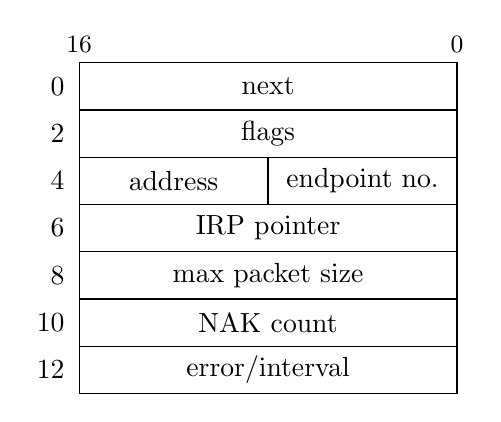
\begin{tikzpicture}[scale=0.3]
  \draw (0,0) rectangle (16,-14);
  \draw (0,-2) -- (16,-2);
  \draw (0,-4) -- (16,-4);
  \draw (8,-4) -- (8,-6);
  \draw (0,-6) -- (16,-6);
  \draw (0,-8) -- (16,-8);
  \draw (0,-10) -- (16,-10);
  \draw (0,-12) -- (16,-12);
  \draw (0,-14) -- (16,-14);
%
  \node[anchor=east] at (-0.2,-1) {0};
  \node[anchor=east] at (-0.2,-3) {2};
  \node[anchor=east] at (-0.2,-5) {4};
  \node[anchor=east] at (-0.2,-7) {6};
  \node[anchor=east] at (-0.2,-9) {8};
  \node[anchor=east] at (-0.2,-11) {10};
  \node[anchor=east] at (-0.2,-13) {12};
  \node[anchor=south] at (0,0) {\small 16};
  \node[anchor=south] at (16,0) {\small 0};
%
  \node at (8,-1) {next};
  \node at (8,-3) {flags};
  \node at (12,-5) {endpoint no.};
  \node at (4,-5) {address};
  \node at (8,-7) {IRP pointer};
  \node at (8,-9) {max packet size};
  \node at (8,-11) {NAK count};
  \node at (8,-13) {error/interval};
\end{tikzpicture}

Fields are as follows.

\begin{description}
  \item[next]  Pointer to the next endpoint.  These structures are meant to
    be arranged in a single-linked list using LL\_APPEND\_ATOMIC from
    utils.s.

  \item[flags]  Bit fields describing the type and status of the endpoint. 
    Constants for the Gracious Host-defined bit fields are in global.inc as
    symbols starting EPF\_ and EPFM\_.  The \emph{high byte} of this word
    (byte at offset 3) is a copy of the 8-bit \emph{bmAttributes} field from
    the USB endpoint descriptor returned by the device.

  \item[endpoint no.]  The byte at offset 4 is the 8-bit endpoint number on
    the device to which this structure connects.

  \item[address]  The byte at offset 5 is the 8-bit USB bus address of the
    device.  The Gracious Host always sets this to 1 during enumeration. 
    The reason for storing it in the EP structure at all is that bytes 4 and
    5 together form a 16-bit word in a format the hardware wants to see; and
    for the earliest control transfers that actually perform the
    enumeration, it may need to be zeroed.

  \item[IRP pointer]  Address in RAM of the IRP data structure (next
    subsection) that this endpoint is currently processing.

  \item[max packet size]  Maximum packet size the device supports for this
    endpoint, as it reported during configuration.  Set to guessed constants
    in early transfers, before the device has actually told the host what
    size it supports.

  \item[NAK count]  Count of the number of NAK packets, used for detecting
    the ``too many NAKs'' error condition on endpoints that do not allow
    infinite NAKs.

  \item[error/interval]  Normally, an error code.  Values are defined in
    global.inc, and some of them are set by the hardware.  A zero value,
    called ERR\_SUCCESS, corresponds to no error.  The occurrence of an error
    is also indicated by the IRPF\_ERROR bit in the IRP (not EP) flags
    field.  The EP error field is
    overloaded by the subroutines that configure INTR endpoints, to return
    the number of milliseconds at which the device requests to be polled. 
    The calling driver is expected to pick up this value from the field
    and store it somewhere safe before actually using the newly-configured
    endpoint, at which time the field will be used normally for error
    codes.
\end{description}

\subsection{I/O Request Packet (IRP)}

Another data structure used for communication between per-device drivers and
the low-level USB subsystem is called the I/O Request Packet (IRP).  Each
IRP describes a request for a transfer to or from the USB device.  The IRP
is separate from the EP so that a driver can maintain several of them for
different frequently-used kinds of transfers, and point the EP to different
IRPs to easily switch between them.

The IRP consists of an 8-byte header which points to a buffer.  For control
transfers in particular, the buffer is expected to immediately follow the
header, and to contain eight bytes at the start for the SETUP message
followed by space for the data payload if any.  For other types of transfers
(that is, interrupt and bulk; isochronous are not supported), the buffer may
be anywhere in RAM.

\pagebreak
Here is the IRP layout.

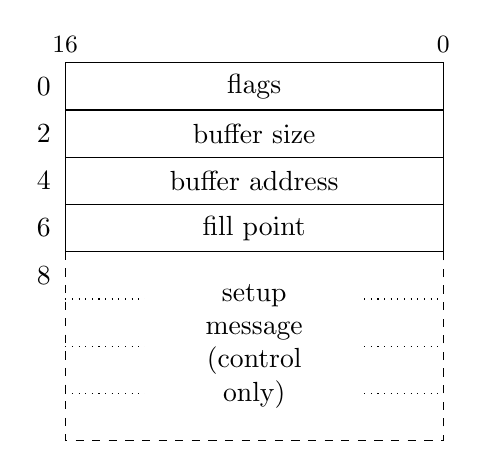
\begin{tikzpicture}[scale=0.3]
  \draw[dashed] (0,-8) rectangle (16,-16);
  \draw (0,0) rectangle (16,-8);
  \draw (0,-2) -- (16,-2);
  \draw (0,-4) -- (16,-4);
  \draw (0,-6) -- (16,-6);
  \draw[dotted] (0,-10) -- (16,-10);
  \draw[dotted] (0,-12) -- (16,-12);
  \draw[dotted] (0,-14) -- (16,-14);
%
  \node[anchor=east] at (-0.2,-1) {0};
  \node[anchor=east] at (-0.2,-3) {2};
  \node[anchor=east] at (-0.2,-5) {4};
  \node[anchor=east] at (-0.2,-7) {6};
  \node[anchor=east] at (-0.2,-9) {8};
  \node[anchor=south] at (0,0) {\small 16};
  \node[anchor=south] at (16,0) {\small 0};
%
  \node at (8,-1) {flags};
  \node at (8,-3) {buffer size};
  \node at (8,-5) {buffer address};
  \node at (8,-7) {fill point};
  \node[fill=white] at (8,-12)
    {\parbox{1in}{\centering setup\\message\\(control\\only)}};
\end{tikzpicture}

The fields are as follows.

\begin{description}
  \item[flags]  Bits describing the type and status of the request. 
    Note in particular that there is a UOWN flag for handshaking between the
    foreground and ISR in software, much like the handshaking between the
    software and hardware on BDT entries.  Constants for the bit fields are
    in global.inc as symbols starting IRPF\_ and IRPFM\_.

  \item[buffer size]  Size of the buffer.  This controls the transaction
    size.  The number here should include the setup message
    for control transactions (eight bytes), and any data payload.  Because
    the hardware sometimes overruns on DMA writes, it is advisable
    to actually allocate seven or eight bytes of padding after the
    buffer, which are not counted in the number of bytes stored here.

  \item[buffer address]  Address in RAM of the start of the buffer.  For
    \emph{control} transfers, this must point immediately after the IRP
    header structure (that is, at offset 8 from the start of the header). 
    For other transfers it may point anywhere.

  \item[fill point]  Offset into the buffer (that is, byte count, not
    address) of the next byte to transfer, or immediately after the last byte
    transferred.  Note that for control transfers, this will be 0 until the
    setup message is sent, then starts at 8 for the data bytes.

  \item[setup message]  The 8-byte setup message (for control transfers
    only) is formatted as described in the USB standard.
\end{description}

\section{Initialization and finalization}

The USB\_INIT subroutine sets up the USB hardware to listen for a device
attach.  It basically just loads appropriate values into the SFRs and turns
on the interrupts for device attach and 1\,ms timing.  Note that the USB
hardware potentially provides two different 1\,ms interrupts:  the ``On The
Go'' 1\,ms interrupt, which is available at all times and is the one turned
on here, and the ``SOF'' interrupt, which is only available when actually
sending SOFs or keep-alives to an attached USB device.  The SOF interrupt is
more accurately 1\,ms.  The Gracious Host switches between the two, using
the SOF interrupt for timing when possible but the 1\,ms interrupt at times
like these when SOF/keep-alive generation cannot be turned on.

USB\_DONE is even simpler:  it just turns off USB interrupts, clears a few
control registers, and clears the soft USB\_FLAGS variable.  If there should
still be a device attached at this point, the lack of SOFs or keep-alives
from the host will cause it to automatically shut down after a few
milliseconds.

Calling USB\_INIT when there is already a USB session in progress will break
the session off ungracefully, but should be safe from the driver's point of
view as long as the foreground keeps track of its own memory allocations and
other state.  It may be best not to do this while there is a \emph{transfer}
in progress, because the initialization includes the BDT and the hardware
could be attempting DMA at the time.  Calling USB\_DONE when there is no
session in progress, or when there has been no matching USB\_INIT call,
should be safe.

\section{Session handler}

The progress of the USB \emph{session}, from attach to detach, is handled by
the subroutine USB\_HANDLE\_SESSION.  Normally, the main loop in firmware.s
calls USB\_HANDLE\_SESSION when USB\_TEST\_ATTACHED returns NZ status; it is
expected, though not guaranteed in case of error, that the session handler
will remain in control until the USB device detach.  It ought to THROW in
case of an error that cannot be handled within the driver, but firmware.s is
also prepared to handle a simple return in an abnormal state, with the
device still attached.

The session handler is assembled into specially-named sections, not the
default .text, so that the customized linker script can insert code
fragments from other files to build up the executable TDL and TIL.  Devices
have device descriptors which say what kind of device they are, and code in
the TDL can match on those descriptors to call a driver for the entire
device.  Devices also have (potentially multiple) ``configurations,'' each
of which may contain (potentially multiple) ``interfaces,'' and each
\emph{interface} gets passed to the TIL for a possible match.  There is no
intermediate-level list for matching configurations; the matching is always
on the device or an interface, although an interface match will result in
the firmware selecting the associated configuration when setting up the
device.

\subsection{Sequence of events}

Several things have to happen in a specific sequence at the start of the
session to properly set up the USB device.  Here's a summary.  The structure
of the code follows the sequence quite closely.

\begin{itemize}
  \item Upon device attach, the session handler runs.  The caller has set
    both LEDs green.
  \item There is a 100\,ms pause for the power to stabilize.
  \item Check for low or full speed (USB\_TEST\_SPEED).  This point seems to
    be the only safe one for making this test; I had a lot of trouble trying
    to check the speed at other points in the sequence.  The left LED goes
    red if low speed.
  \item Send ``reset'' for 50\,ms.  Right LED goes red at the start of
    ``reset.''
  \item Start of SOF/keep-alive generation.  100\,ms pause for reset
    recovery.
  \item Prepare the static EP structure for endpoint~0, and a blank IRP
    structure in a \insn{lnk}/\insn{ulnk} stack frame.
  \item Reconfigure interrupts:  OTG 1\,ms off (from this point timing will
    use the SOF interrupt); SOF interrupts on; transfer complete, error, and
    detach on.  The ``detach'' interrupt flag is cleared first to ignore any
    stray detaches signalled prior to this point.  Sometimes contact bounce
    as the plug is inserted causes these.  If the device really detached
    during the roughly 250\,ms elapsed since attach was detected, and has
    remained detached, then that fact will be detected anyway as soon as the
    interrupt is enabled, because of the \emph{level-triggered} nature of
    the detach interrupt.
  \item ``Enumeration'':  do a zero-byte CTRL transfer telling the device
    that its address is~1 (unconditionally).  Call to do\_ctrl\_z\_transaction.
  \item Wait 5\,ms for the device to recover from enumeration.
  \item Do a CTRL read transfer for first~8 bytes of the device
    descriptor; call to do\_ctrl\_r\_transaction.
  \item Extract the actual size of the device descriptor from the 8-byte
    prefix just obtained.  It will almost certainly be~18 bytes, but doing
    this two-step process seems to be the expected procedure.  Do a CTRL
    read transfer for the entire device descriptor.  Copy the device
    descriptor (or, anyway, an 18-byte block from the buffer) to the local
    common-data variable saved\_dev\_desc to preserve it during TPL
    processing.  Update max packet size for EP~0 from the value in this
    descriptor.
  \item Check the device descriptor against the TDL (whole-device portion of
    the TPL).  The low-level driver sets up an exception frame and the TDL
    code is expected to THROW in case of a match.
  \item The linker inserts TDL fragments from all the drivers inside the
    exception frame.  The exception handler, if reached because of the THROW,
    jumps to the per-device driver which the TDL fragment selected by setting
    W4.  The exception handler also turns off the LEDs.
  \item Without a THROW, the session handler starts looping over
    configuration descriptors, using the count of configurations from the
    saved device descriptor.
  \item Request (EP max packet size) bytes of the current-index configuration descriptor with a
    CTRL read transaction.  Find the descriptor's actual size from the first
    few bytes; skip to the next one if it is too long for our buffer. 
    Buffer size is set to accommodate MAX\_DESCRIPTOR\_SIZE set in
    global.inc, currently 1023 bytes, plus appropriate headers and padding. 
    Descriptors we can reasonably use should never be longer than that.
    If descriptor is not too long for buffer, then request all of it with
    another CTRL read.  Save the start of this configuration descriptor (10
    bytes) in the common-data variable saved\_conf\_desc.
  \item The configuration descriptor is a pile of miscellaneous structures
    including its own header, one or more interface descriptor headers, and other
    things nested inside the interface descriptors.  Every item in the pile
    is tagged with a magic number saying what it is (though we do not
    necessarily understand all the types) and its length, and these
    fields are consistently laid out even if the rest of the item is opaque. 
    So there is a chunk of code to ``eat'' a descriptor from the bottom of
    the pile, moving everything after it down however many bytes to bring
    the next item to the start of the data buffer (right after the setup
    message).  This operation gets repeated until there is an interface
    descriptor header at the start of the buffer.
  \item Check the interface descriptor against the TIL.  As with the TDL,
    the session manager sets up an exception frame and the TDL entries from
    per-device drivers get inserted inside the frame by the linker.  If one
    THROWs, then the appropriate driver gets control, through the exception
    handler's \insn{goto}~W4 instruction.
  \item If no THROW, then the session handler loops around, removing items
    from the buffer until there is an interface descriptor at the start.  It
    knows how many interface descriptors are meant to exist in total, from a
    count in the saved configuration descriptor.
  \item If it gets through all the interface descriptors without a match, it
    loops to the next configuration descriptor.
  \item If still no match after the loop over all configurations, the
    session handler sets up an error display with the LED blinker driver,
    and waits for the device to be detached before returning.  This code is
    mingled with a very small ``per-device driver'' for hubs (recognizing
    them on the basis of device descriptor, with a high-priority TDL entry),
    which sets up a different blinking error display and then waits for
    disconnect before returning.
\end{itemize}

There are a few extra globally-visible labels inside the session handler code:
SKIP\_PAST\_INTERFACE
and SKIP\_PAST\_CONFIGURATION, which are at the ends of the associated loops
and possibly useful to TPL entries that try to be ``clever'' about
overriding the usual priority scheme; COMPLAIN\_ABOUT\_DEVICE, which gives
the ``unsupported device'' error display (possibly useful, again, for a TPL
entry that detects a device \emph{known} to be unsupportable); and
ULNK\_RETURN and RETURN\_INSN, which are general-purpose helpers
described in the ``programming tips'' chapter.

\subsection{Interface to TPL entries}

\emph{TPL entries} are fragments of code that per-device drivers can define
in magically named assembly-languge sections.  The linker will insert the
entries into the session handler at the appropriate points, with the
possibility for defining a priority order among entries by the choice of
section names.  Details of the section naming scheme are covered in the
``programming tips'' chapter of this manual.  TPL entries may be designated
for insertion in the TDL (targeted device list, meaning they look at device
descriptors) or the TIL (targeted interface list, meaning they look at
interface descriptors).

The general function of a TPL entry is to look at the current device or
interface descriptor, which will be found starting at address
W14+IRP\_SIZE+8 (that is, offset 16 in the current \insn{lnk}/\insn{ulnk}
stack frame, after the IRP header and setup message) and decide whether the
driver wants to accept responsibility for the currently inserted device on
the basis of that descriptor.  If this driver does want to handle this
device, the TPL entry should THROW, with the entry point of the driver
stored in W4.  If it does a jump instead of a THROW, then the driver will
need to clean up the exception frame by calling TRIED.  There are some
support routines provided for common types of TPL entries, so that usually
an entry will just be a few instructions to set up registers and then make a
call.

TPL entries must preserve the stack context (W14, W15, and the data they
point to) and must return the driver address in W4 when doing the THROW in
case of match, but otherwise are free to overwrite the working registers. 
The registers W4, W5, and W6 are typically used as input arguments to the
support routines.  Support routines are global symbols starting TPL\_.  The
standard ones are as follows.

TPL\_MATCH\_DEVICE\_CLASS is for matching \emph{device} descriptors, in the
TDL, on the
basis of their USB ``class'' and ``subclass'' bytes.  For example, the tdl10
section defined in usb.s recognizes all devices of class~9, which are USB
hubs, to THROW to a stub driver that puts up an error display.  When calling
this routine, put the driver address in W4 and a matching mask in W5:
descriptor class value in the low byte and subclass in the high byte, with
either of them possibly 0xFF as a wildcard that will match anything.  So for
the hub entry, which matches all devices of class~9 regardless of subclass,
the value for W5 is 0xFF09 and the code is as follows.
\begin{tabbing}
\qquad\=\qquad\qquad\=\kill
\>\insn{mov}\>\#handle(complain\_about\_hub), W4\\
\>\insn{mov}\>\#0xFF09, W5\\
\>\insn{rcall}\>TPL\_MATCH\_DEVICE\_CLASS\\
\end{tabbing}

TPL\_MATCH\_INTERFACE\_CLASS is for matching \emph{interface} descriptors, in
the TIL, according to ``class'' and ``subclass'' much in the manner of
TPL\_MATCH\_DEVICE\_CLASS.  It needs to be a separate routine because of the
different layout of device and interface descriptors.  As with the device
version, the driver address goes in W4 and the class and subclass go in W5,
with class in the low byte, subclass in the high byte, and 0xFF serving as a
wildcard.  For example, the USB-MIDI driver's TIL entry sets W5 to 0x0301
and calls this routine to match interface descriptors that name class~1
(``audio''), subclass~3 (``MIDI streaming'').

TPL\_MATCH\_CLASS\_AND\_PROTOCOL is like TPL\_MATCH\_INTERFACE\_CLASS,
but it also tests the ``protocol'' byte from the descriptor against the low
byte of W6.  For example, the boot mouse driver uses this routine to check
for an interface of class~3 (``human interface device''), subclass~1
(``boot''), protocol~2 (``mouse'').

\subsection{Calling convention for per-device drivers}

Because per-device drivers are normally entered by a dynamic \insn{goto}
from an exception handler, they are entered in the stack and exception
contexts that applied immediately before the corresponding TRY.  That means:
\begin{itemize}
  \item upon entry to the driver, there is a \insn{lnk} stack frame in
    effect, containing a leftover IRP, setup message, and what remains of
    the descriptor pile; the driver may still have a use for that in calling
    some setup utility subroutines, which may implicitly do \insn{ulnk}, but
    must do \insn{ulnk} one way or another before returning if it returns
    with \insn{return} instead of an exception;
  \item configuration of the device, in the USB sense of sending it a
    SetConfiguration command, still must be done;
  \item if and only if the driver was entered from the TIL (matching an
    interface descriptor as opposed to a device descriptor), then the
    low-level driver has the configuration descriptor containing the current
    interface descriptor memorized in internal static variables accessible
    to the support routines;
  \item returning from a driver with \insn{return}, after cleaning up the
    stack frame, returns to the caller of
    USB\_HANDLE\_SESSION, under non\_usb\_done in firmware.s;
  \item returning with \insn{return} is expected only after the device has
    detached, because if it is still attached, then the attached device will
    be immediately detected again and the session handler will run again; and
  \item exceptions thrown by a driver are handled by catch\_usb\_session in
    firmware.s, and the driver is expected to THROW if there is an error
    so serious it cannot recover, whether the device has detached or
    not, or on a normal detach if that is detected implicitly during a call
    to USB\_WAIT\_ON\_IRP.
\end{itemize}

Most per-device drivers call a configuration support subroutine that
implicitly removes the session handler's \insn{lnk} frame, possibly they
create a new frame of their own, and then they enter an infinite loop with
no explicit return.  They call USB\_WAIT\_ON\_IRP inside the loop, which
implicitly checks for device detach.  Normal operation continues either
until power-down or until the device detaches, in which case
USB\_WAIT\_ON\_IRP detects the detach and does a THROW.  The THROW
terminates the driver and cleans up the stack.  So there is very little
explicit handling of detach, termination, or stack frames inside the driver. 
That all happens automatically as a result of calling the support routines. 
The USB mass storage driver, which in normal operation does not return at
all (because firmware update ends in a global \insn{reset}), handles the
stack in a somewhat more complicated way.

Per-device drivers have basically free use of the working registers and any
module hardware that does not have permanently fixed configuration.  The
firmware framework re-initializes as necessary any devices that drivers
might reasonably want to reconfigure (such as output compares), when it
regains control.  Per-device drivers have free use of the common data area,
after they have completed any calls to the configuration helper APIs (which
use information left by the session handler in the common data area).  There
are some conventions for common-data usage on calls \emph{between}
per-device handlers, which are out of scope of this chapter.

\section{Foreground transaction processing}

The global subroutine USB\_WAIT\_ON\_IRP is the main API for other drivers
to make USB transactions.  It requires an EP and an IRP to exist in RAM. 
The endpoint should be already initialized, and the buffer address field of
the IRP, but this routine sets up the other fields of the IRP using
arguments from working registers, because its loop needs to repeatedly
reinitialize these fields anyway.
 
Put the configuration flags (OR of IRPFM\_ constants) in W1.  Put the buffer
size in W2, the EP address in W4, and the IRP address in W5.  This routine
may trash W0 and W3.

Depending on the type of transaction, USB\_WAIT\_ON\_IRP may take a long
time to return; with USB bulk transactions in particular, it will wait for
data to be available, which has no time limit.  There is special support for
calling the MIDI\_BACKGROUND\_SAFE subroutine from midi.s inside the loop to
keep the backend's ongoing tasks running while waiting for more input data;
set the UF\_MIDI\_BKGND bit in USB\_FLAGS to enable this feature, and do so
only after the MIDI backend driver has been initialized.  Also inside
USB\_WAIT\_ON\_IRP's loop, there is a check for device detach, which will
result in an exception THROW.  Errors as such, reported by the hardware,
will be retried five times and then also result in a THROW.  When doing an
error retry, the loop unconditionally clears the EP's ``stall'' flag.  It
does a normal \insn{return} if the USB transaction succeeds.

There are several more non-globally-visible entry points used for CTRL
transactions within usb.s.  They just put commonly-used values into the
argument registers before jumping or falling through to USB\_WAIT\_ON\_IRP,
so that these values need not be specified repeatedly everywhere.  Note that
a CTRL transaction with no data in either direction (referred to as
``ctrl\_z'' in the code, for zero data bytes) is treated by USB as a
\emph{write} of length zero.

\section{TPL support routines}

The support APIs for TPL entries are described above; this code is mentioned
again here to follow the sequence of the source file.  The exception handler
active during TPL processing is just three instructions to turn off the
front-panel LEDs and jump to the driver address that should be in W4.  The
three TPL\_MATCH\_ subroutines have a support routine of their own for doing
the 0xFF wildcard match, and they share a lot of code with each other.

\section{Device driver support routines}

The subroutines in this section send specific control transactions to the
USB device that are (or could be) shared by multiple per-device drivers. 
They are intended to be called soon after the driver receives control from
the TPL.

USB\_CONFIGURE\_DEVICE tells the device to use the current
``configuration,'' as described by the interface descriptor in the
\insn{lnk} stack frame and memorized during TPL processing.  \emph{It then
removes this stack frame.} Drivers that want a stack frame of their own
should do their \insn{lnk} after the call to USB\_CONFIGURE\_DEVICE.  On
entry, W8 should point at an array of EP structures, with W9 containing the
count of how many EPs are in the array.  Most per-device drivers are
expected to set W8 and W9 and then call this routine as the first thing they
do.

USB\_CONFIGURE\_DEVICE initializes the EPs according to the descriptions of
endpoints in the descriptor, in the order that they occur in the descriptor,
up to the length of the array or up to the number of endpoints described in
the descriptor.  If the array is too short to contain all the endpoints from
the descriptor, then the additional endpoints are ignored; and if the array
is longer than necessary to contain all the endpoints, then the remaining
array entries are left uninitialized.  On return, the W8 register is left
pointing just after the last EP structure that was actually filled.  The
reason for this behaviour is that interfaces commonly list the basic,
standard, or required endpoints first in the descriptor, and then optionally
extra endpoints later.  So a driver that only supports basic features can
ask for just the first one or two endpoints and be likely to get the ones it
wants, whereas a more sophisticated driver can ask for more, and then detect
whether the device offered the more advanced ones.

Note that although devices \emph{do} commonly put required endpoints first
and optional ones later, devices do \emph{not} necessarily follow a specific
convention for the order of input and output endpoints on interfaces that
include both.  The driver that supports a bidirectional interface (or
possibly even a unidirectional interface with more than one endpoint) will
need to dig through the array to figure out which endpoint is which; see
FIND\_IN\_OUT\_ENDPOINTS in qwerty.s for relevant code.

USB\_SET\_BOOT\_PROTOCOL is specifically for Human Interface Devices that
support a ``boot'' protocol, namely mice and typing keyboards.  It makes a
SET\_PROTOCOL request for protocol 0, selecting the simplified protocol that
the USB organization proposed for use during PCs' boot processes.

USB\_SET\_REPORT does a SET\_REPORT operation for a HID, with the single byte
of data from W2 low.  This is used by typing keyboards to set the LED state.
In the current firmware it is not used elsewhere, but could be relevant for
other HIDs.

\section{General USB APIs}

The routines in this section do low-level things related to timing and bus
status that may be of interest to per-device drivers, particularly for
calling within a driver's main loop.

USB\_TEST\_ATTACHED makes sure that the device is still attached, and
incidentally, confirms that the bus voltage is okay with a call to
CHECK\_VBUS.  Calling this regularly fulfills the driver's obligation to
keep an eye on V$_\textrm{BUS}$.  It returns the result in the CPU's zero
flag, so upon return it can be tested with \insn{bra z} or \insn{bra nz};
non-zero means the device is attached.  As a side effect, in case of
disconnection USB\_TEST\_ATTACHED will also set the disconnected error code
on the current EP if any, and the error bit on the currently in-progress
IRP, if any.  This is incidentally where the Z\_RETURN and NZ\_RETURN
general utility labels are defined.

The internal labels referring to ``confirm''(ing) attachment and detachment
are left from an earlier version that attempted to go all the way to the
hardware, in foreground code, to check whether the device was attached or
detached.  I found that approach unreliable and the current version just
looks at the soft UF\_ATTACHED flag in USB\_FLAGS, which is maintained by
the ISR.  The attach/detach interrupts seem to be the only trustworthy way
of knowing whether the device is attached.  Driver code that wants to really
\emph{just} check for whether the device is attached or not, without the
side effects of USB\_TEST\_ATTACHED, could also look directly at the
UF\_ATTACHED flag; but the side effects of calling USB\_TEST\_ATTACHED are
usually desirable in practice.

USB\_TEST\_SPEED still does go all the way to the hardware to test whether
the device is low-speed or high-speed.  This approach \emph{is} unreliable
unless the check happens at exactly the right point in the
attach/enumeration process.  Since it works by examining the ``idle''
voltages on the bus, which are different between low and full speeds, it can
only read a correct answer when the bus actually is idle.  The subroutine
attempts to improve reliability by waiting until the hardware gives the same
answer in three consecutive checks at intervals of approximately
USB\_BUS\_SETTLING\_TIME instruction cycles (each 62.5\,ns; recommended value
24, which is 1.5\,$\mu$s).  But even with this measure, the call to
USB\_TEST\_SPEED should normally be done only by the session manager, and
per-device drivers should instead look at the UF\_LOW\_SPEED flag in
USB\_FLAGS.  As side effects, USB\_TEST\_SPEED sets that flag and the
hardware's configuration bits (LSPDEN in U1ADDR and LSPD in U1EP0) according
to the detected speed.  Note that it is important to configure \emph{both}
the LSPDEN and LSPD bits, to match each other and the device; disagreement
among them causes confusing problems.

USB\_WAIT waits, for a number of milliseconds specified in W0.  It actually
waits for \emph{the millisecond interrupt to occur} W0 number of times,
which means the real time between the call and return could be almost a
millisecond less than the W0 value.  The ``millisecond interrupt'' is either
the USB OTG 1\,ms interrupt, or the SOF interrupt, depending on whether SOF
generation is currently turned on.  Per-device drivers will normally only be
running while a device is attached, so SOF generation will be on and they
will be getting the SOF interrupt, which in my tests seems to give more
accurate timing.  But the low-level driver also supports use of the USB OTG
1\,ms interrupt so that it can call USB\_WAIT during the attach process, when
SOF is turned off.

USB\_LOOP\_WAIT is similar, but uses a \emph{soft timer} that counts
interrupts even while outside a call to USB\_LOOP\_WAIT.  The concept is
that repeated calls to USB\_LOOP\_WAIT with a given W0 value will return W0
number of milliseconds apart, even if the foreground processing between
calls to USB\_LOOP\_WAIT may consume more than one millisecond.  If the
scheduled time is already overdue when this routine is called, it returns
immediately, resetting the timer for a full W0 number of milliseconds before
the next return.  This routine will also call the MIDI background task
within its loop, if the UF\_MIDI\_BKGND flag is set in USB\_FLAGS. 
Per-device drivers for devices with ``interrupt'' endpoints, which are
supposed to poll the device a given number of milliseconds apart, can call
USB\_LOOP\_WAIT to handle their poll timing with very little other effort
required.

USB\_LOOP\_CHECK is a variation on USB\_LOOP\_WAIT that does not wait but
only \emph{tests} whether a scheduled poll is due, returning NZ if it is due
and Z if not.  This behaviour would be appropriate for a driver that has
lower-priority things it can do while waiting for the poll. 
USB\_LOOP\_CHECK does not run the MIDI background.

Calls to USB\_LOOP\_CHECK and USB\_LOOP\_WAIT use the same timer and may be
mixed.  It is normally expected that a driver will always use the same W0
value for these two routines, at least for a given device, or at the very
least, that it will only infrequently change the value of W0.  If the W0
value changes from one call to the next, USB\_LOOP\_CHECK or USB\_LOOP\_WAIT
may skip a poll or trigger an extra poll, but should not misbehave beyond
that.

\section{The token store}

The USB standards allow, but do not require, hosts to poll device bulk
endpoints at any time the bus is not scheduled to be used for some other
purpose.  If permitted to retry each failed poll immediately, the Gracious
Host firmware is capable of polling at upwards of 40\,kHz.  Polling so often
seems undesirable.  The bulk endpoints of devices this host is intended to
support are those on USB-MIDI and mass storage devices.  The former only
produce data when there is MIDI traffic (usually at most a few hundred
bytes, fewer messages, per second) and the latter often go quiet for many
milliseconds at a time due to the delays of reading flash memory, hard
drives, or similar.  So polling more than a few times per millisecond has no
useful effect, and it consumes extra power, possibly loads down the
microcontrollers at either end of the bus (slowing their ability to do other
tasks), and may contribute to EMI.  Conducted EMI from USB devices is often
an issue in modular synthesizers and I would prefer to keep the USB device
no busier than necessary.

The Gracious Host firmware attempts to reduce the polling rate to a more
reasonable level without harming response time by implementing a \emph{token
store} for USB polling.  The global variable TOKEN\_STORE records how many
tokens the low-level driver is currently permitted to send before waiting. 
Each time the ISR sends a token it subtracts one from TOKEN\_STORE, and it
will not send a token if TOKEN\_STORE is zero.  The global variable
TOKEN\_ALLOWANCE will be added to TOKEN\_STORE once per millisecond. 
\emph{Note that TOKEN\_ALLOWANCE defaults to zero.} USB\_WAIT\_ON\_IRP
forces TOKEN\_STORE to 0xFFFF inside its waiting loop.

Most drivers communicate with the USB hardware only through
USB\_WAIT\_ON\_IRP (directly or inside other APIs), so the token store has
no important effect on most drivers.  It just gets topped up to 0xFFFF each
time through the loop and is never expected to reach zero.  But the USB-MIDI
driver, which implements its own waiting loop and calls USB\_POKE, interacts
with the global variables to limit its bulk endpoint polling rate to
(nominally) two polls per millisecond, plus an additional one each time
through the MIDI background processing.

\section{Packet send and poke}

Several different code paths result in the host attempting to send a token
on the USB bus.  A token attempt might occur after an SOF interrupt because
the foreground has queued a request for a transfer; after a failed earlier
token, to retry it; after a successful earlier token, to proceed to the next
step in a multi-step transaction; or when explicitly requested by the
foreground.  These code paths converge on the send\_next\_token label in
usb.s.  The low-level driver's packet-sending all originates in the USB
multiplex ISR; but there is also the potential that foreground code might
want to get a queued transfer started immediately, without waiting for an
interrupt, and the USB\_POKE subroutine provides access to send\_next\_token
from foreground code for this purpose.  Calling USB\_POKE tells the driver
that now is a good time, from the foreground's point of view, to send a
token if it happens to have a token it wants to send.

The send\_next\_token routine expects W1 to point at the EP data structure
of the current transaction, if any; USB\_POKE automatically sets W1 from an
internal variable and resets it to the start of the list if the list is
completed, but some paths in the ISR use this register to have the new token
be a response to an earlier token on the same endpoint as a previous token.

First there are some general checks:  whether the global UF\_BUSY bit is set
(indicating a token is currently in progress, so we cannot start another)
and whether we have reached the end of the endpoint list (indicating no
further work to do).  Either of these result in an immediate return. 
Otherwise, send\_next\_token loops over the endpoint list looking for one
that is not marked ``stalled'' and that has an active IRP with the
IRPF\_UOWN flag bit set (indicating that the foreground has given ownership
of that IRP to the low-level driver).

For CTRL transactions:  the UF\_SENT\_CTRL bit gets checked.  Only one CTRL
transaction is allowed per frame, so this bit is set on the first CTRL
transaction of the frame to prevent a second one from happening.  It is
reset by the ISR on the SOF interrupt.  If it is found already set here,
control goes back to send\_next\_token to look for something else to send.
Otherwise, the code consumes a token from TOKEN\_STORE, aborting if there
are none remaining, and checks the current stage of the transaction.

The first stage of a CTRL transaction is the SETUP token.  In this case, the
code confirms the outgoing BDT entry is not already occupied (should never
happen, but just in case), and then sets up the BDT entry with the
appropriate flags, buffer size, and buffer pointer read from the IRP.  It
also saves the pointers to the current EP and IRP pointers in the variables
tx\_ep and tx\_irp.  Then it writes to the hardware registers to tell the
USB hardware to send the token, and branches to finished\_sending\_ctrl.

The second stage of a CTRL transaction is the DATA stage.  This is optional,
conditioned on whether there was space for data declared in the IRP.  Many
CTRL transactions send all their information in the eight-byte SETUP packet
and skip the DATA stage.  But, if a DATA phase is in order, the code sets up
the BDT for one packet of data transfer.  That will be a maximum-length
packet if the remaining buffer (from fill point to end) is at least the
maximum packet length, and otherwise it will be a packet covering the rest
of the buffer.  The code covers both read and write using test-and-skip
instructions to handle the few differences between the two directions. 
Basically, it just points the hardware at the buffer and tells the hardware
to do the transfer.  Then this path also branches to finished\_sending\_ctrl.

With or without a DATA stage, the CTRL transaction ends with the ACK stage,
which is effectively a zero-length DATA transfer in the opposite direction
from the main CTRL DATA transfer.  CTRL transactions with no DATA stage are
counted as if they were writes for this purpose, so the ACK stage in such a
case is a read.  The code for this stage is very similar to the DATA stage
code, just with different length calculation because the length is known to
be zero, and the special handling of USB's DATA0/DATA1 handshake bit
required for the ACK stage.  Then it falls through to
finished\_sending\_ctrl.

The finished\_sending\_ctrl label wraps up handling any of the stages of the
CTRL transaction.  It sets the UF\_SENT\_CTRL and UF\_BUSY flags to indicate
that a CTRL transaction has been sent in this frame (so no more are allowed)
and that a transaction is currently in progress.  Depending on
conditional-assembly directives, it resets the UF\_BUSY watchdog and sends
the test point GPIO pin high.  Both these measures are intended for debugging
issues with the scheduling of when the USB subsystem goes or stays busy. 
Then it returns, ending send\_next\_token.

Transactions other than CTRL transactions are necessarily INTR or BULK
transactions, because we do not support isochronous endpoints.  Both of
these are handled starting from the label try\_sending\_intr\_bulk.  As with
CTRL, this code starts by consuming a token from TOKEN\_STORE and aborting
if there are none.  From there, the code is very similar to that used for
CTRL DATA.  It finds a block of the buffer to send or receive (one
maximum-length packet or the rest of the buffer, whichever is less), sets up
the BDT entry to point at that block, saves the EP and IPR pointers, and
sends it to the hardware.  Then it branches back to share part of
finished\_sending\_ctrl, setting UF\_BUSY and optionally resetting the
watchdog and sending the test point GPIO high before returning.  The
differences between sending and receiving, and betweem INTR and BULK, are
small enough that the same code can handle all four
possibilities with just a few conditional-skip instructions to handle the
differences.

\section{Multiplex ISR}

The PIC24 USB hardware includes a dedicated interrupt controller of its own
that multiplexes all the USB-related interrupts onto a single interrupt of
the main PIC24 interrupt controller.  So the ISR for that interrupt has to
look at the hardware registers to figure out which interrupt source actually
caused the interrupt -- potentially many, because multiple sources could be
active simultaneously.

The ISR starts by saving registers W0--W5, acknowledges the PIC24 interrupt
(as is required in all PIC24 ISRs), and then proceeds to examine each of the
interrupt sources of interest to the low-level driver.  The section for each
interrupt source starts with local label ``6:''; it tests the relevant bits in
the hardware registers for whether the source is enabled and requesting an
interrupt, and if not, skips to the next ``6:'' using the name ``6f.''  If
the interrupt source is detected and handled, then the section will normally
fall through into the next section so that multiple interrupt sources can be
handled in a single call to the multiplex ISR.

Note that interrupt-request bits in the USB hardware's dedicated interrupt
controller work a little oddly: to \emph{clear} them, we must write a 1 to
the bit position (usually in the U1IR register).  It may not be safe to use
\insn{bset} on U1IR because that works by reading the register value,
setting the bit, and writing the changed value -- so if other bits are 1,
those may also be cleared by \insn{bset}.  (I write ``may'' because I have
not tested this expected misbehaviour on real hardware.) The safe and
recommended thing to do for clearing a bit in U1IR is to write the register
without reading it, such as with \insn{mov}~W0, U1IR, using a constant value
that is 1 in exactly the bit position(s) one wants to clear.  This ``write 1
to clear'' behaviour is distinct from that of interrupt-request bits in the
main PIC24 interrupt controller, which are simply register bits that can be
cleared normally.

\subsection{Attach}

The attach interrupt comes in when the user inserts a USB device.  Turning
on the USB hardware with a device already inserted also causes this
interrupt.  And, as semi-documented by Microchip, the attach interrupt is
\emph{level triggered}, which means that it will happen again as soon as it
is acknowledged, if the device is still attached and the interrupt is still
enabled.  Unlike PIC24 interrupts in general, which only need to be
acknowledged by clearing the interrupt bit, the level triggered attach
interrupt needs to be fully \emph{disabled} when the firmware records that
the device has attached, and that must happen before acknowledging the
interrupt.

Accordingly, the handler for the attach interrupt sets the UF\_ATTACHED bit
in USB\_FLAGS for reference by the foreground; turns off the attach
interrupt, acknowledges \emph{both} the attach and detach interrupts (to
guard against contact bounce and spurious detaches that may have come in
since the last state change), and then enables the detach interrupt.

If the LEDS\_ON\_USB\_ATTACHED debugging symbol is set, then the code also
clears bits 7 and 9 of LATB, to turn the front-panel LEDs red.  It is
assumed they were already turned on, by clearing the corresponding TRISB
bits, by some other code.

\subsection{Detach}

The detach interrupt is handled very much like the attach interrupt. 
Although Microchip does not explicitly document this fact, detach is another
\emph{level triggered} interrupt that must be fully disabled before being
acknowledged.  The code does the opposite steps from attach:  clear
UF\_ATTACHED, disable detach interrupt, acknowledge \emph{both} attach and
detach interrupts, and enable attach interrupt.  If LEDS\_ON\_USB\_ATTACHED
is set, it also turns the front-panel LEDs green.

\subsection{Start Of Frame}

The SOF interrupt happens at 1\,ms intervals whenever SOF/keep-alive
generation is turned on, which is all the time when a device is attached and
in normal operation.  This interrupt actually happens a little before the
SOF (for full speed) or keep-alive (for low speed), just at the moment when
there is \emph{no longer enough time to send a packet} without the packet
colliding with the SOF or keep-alive.  Paradoxically, that is considered the
very best time to tell the hardware to send a packet, because it means the
hardware will hold onto the packet and then send it at the first safe
opportunity, immediately after the SOF or keep-alive, without a gap.  In
combination with things like ping-pong mode (not used in the Gracious Host),
having the interrupt come in when the bus is \emph{not} available helps to
maximize throughput.  Using an interrupt that only came in when the bus was
idle as the stimulus for sending a packet would introduce a delay, with the
bus remaining idle, while the firmware prepared the packet; but the time
pressure on the firmware to get the packet ready for the hardware is
alleviated if the firmware is working while the hardware would be
unavailable anyway.

After acknowledging the interrupt, the SOF interrupt handler calls
handle\_1ms\_tick, which is in a subroutine so it can be reused by the
On The Go 1\,ms interrupt handler below, and described in the documentation
for that handler.  It raises the test point GPIO pin if PULSE\_PIN14\_ON\_SOF
is set; that debugging symbol is of some use in providing an oscilloscope
trigger for inspecting transactions on the USB bus.  Then it clears the
UF\_SENT\_CTRL bit in USB\_FLAGS, to allow a new CTRL token to be sent now
that we have a new frame, and resets the current pointer into the endpoint
linked list to the start of the list.  Finally, it branches to
send\_next\_in\_isr, which calls send\_next\_token and then ends the ISR. 
If there are other interrupt sources remaining, they go unhandled in this
pass through the ISR, but as soon as it returns, the unhandled interrupt
sources will trigger the ISR to run again.

\subsection{On The Go 1\,ms}

The USB hardware supports a second 1\,ms interrupt called the ``On The Go
1\,ms interrupt.'' Its timing seems to be less accurate than the SOF
interrupt, and the two drift relative to each other.  However, the On The Go
1\,ms interrupt can be turned on and off at any time, whereas the SOF
interrupt only happens when SOF/keep-alive generation is turned on. 
SOF/keep-alive generation needs to be turned off sometimes, and the USB
session handler wants to use a millisecond timing interrupt even when
SOF/keep-alive generation is off, so there is a need to use the On The Go
1\,ms interrupt too.  The firmware switches between them, using the SOF
interrupt for timing when it is turned on, and the On The Go
1\,ms interrupt when the SOF interrupt is turned off.

After confirming that the SOF interrupt really is turned off, this handler
calls the handle\_1ms\_tick subroutine, which is shared with the SOF handler
and written inline as a star-section at this point in the source code.  It
does all the recurring tasks needed per millisecond by the USB driver's
timing features.
\begin{itemize}
\item It sets the SI\_1MS flag in SOFT\_INT\_FLAGS, which is used by
  USB\_WAIT to count millisecond interrupts in the foreground.
\item It decrements the millisecond counter used by USB\_LOOP\_WAIT.
\item If UF\_BUSY\_WATCHDOG\_TIME is defined to a positive value, it
  checks whether the hardware and firmware are both reporting ``busy''
  status; if so, decrements the watchdog timer; and if the timer hits zero,
  resets the processor.  Some bugs can cause the bus to lock up in ``busy''
  status more or less permanently, and this watchdog if enabled allows for a
  chance of recovering from such an occurrence.
\item It adds TOKEN\_ALLOWANCE to TOKEN\_STORE, to permit a few more bulk
  polls for drivers that use the token store mechanism.
\end{itemize}

\subsection{Error}

The handler for the USB error interrupt is minimal:  it just clears the
interrupt, and clears the UF\_BUSY flag (lowering the test point GPIO pin if
PULSE\_PIN14\_ON\_BUSY is defined), and jumps to the
after\_transfer\_complete label, which skips past other handling of the
just-completed transaction.  This behaviour will result in the transaction
being retried next time the ISR has a chance to run through the endpoint
list.

\subsection{Shared transfer-complete code}

The \emph{transfer complete} interrupt occurs after a token has been sent
and possible response collected, whether it was successful or unsuccessful. 
The code for this interrupt decodes how the token ended and determines what
to do next, based on the current state of the larger USB transaction and
what type of transaction it is.

First, it collects the current value of the U1STAT regiser (saying how the
token ended) \emph{before} acknowledging the interrupt, because the hardware
is free to rewrite that register as soon as the interrupt has been
acknowledged.  This value is used only to determine whether the
recently-completed token was a ``transmit'' or ``receive'' token,
determining which BDT entry is relevant.  It finds that entry, confirms that
its UOWN bit has been passed back to the software, and extracts the saved EP
and IRP addresses from the associated variables.  The endpoint number of the
token as reported by the hardware is checked against the one in the EP data
structure; if they do not match, the token may represent left-over bus
traffic from an earlier transaction, and is discarded.

Then the code collects the PID value from the BDT entry, which represents
the result of the the token.  The values PID\_ACK, PID\_DATA0, and
PID\_DATA1 all represent a basically successful token and are handled the
same.  In these cases, the EP's EPF\_DATA1 flag bit gets toggled
(meaning that after DATA0 we will expect DATA1 next and vice versa) and the
IPR's fill point gets updated for the newly-transferred bytes (zero being an
allowed number of new bytes, typical of ACK packets).

Then there is some conditional logic to separate the cases.  On CTRL
transactions, if we have sent the ACK then the transaction is done and we
jump to return\_irp\_to\_foreground.  Otherwise, if all bytes have been
transferred, or if the recent packet was zero-length, then it is time to
send the ACK, and we set the IPR's IRPF\_ACK flag bit to indicate that. 
Finally on any CTRL transaction that is not yet complete, whether or not
IRPF\_ACK was set, we jump to finished\_incoming\_packet, which will try to
send the next packet of the transaction (either another data packet, or the
ACK).

If the transaction was not a CTRL transaction, is not complete (not all
bytes transferred yet), and we did not see a zero-length packet, then we
jump to finished\_incoming\_packet to attempt sending or receiving more. 
Non-CTRL transactions that have filled their buffers, or that have completed
the transmission of a zero-length packet in either direction, will end
without further handshaking; in these cases the code jumps or falls through
to return\_irp\_to\_foreground.

The return\_irp\_to\_foreground label is reached by several branches of the
logic and represents the end of a transaction.  It nulls out the pointer in
the EP to the IRP (because this IRP is no longer active), and clears the
IRP's IRPF\_UOWN bit to return responsibility for that IRP to the
foreground.  Then it branches to finished\_incoming\_packet to look for more
work to do.  That concludes handling of basically successful PIDs (ACK,
DATA0, and DATA1).

The NAK PID is next.  USB specifies this PID for several cases that
basically amount to a transaction \emph{temporarily} failing.  NAK should
result in at least a limited number of retries, unlimited for some
transactions.  Accordingly, we check the EP's EPF\_INFINITE\_NAK flag and if
it is set, branch to finished\_incoming\_packet to make another attempt. 
Otherwise, we increment the EP's NAK counter.

On an INTR input transaction, NAK is actually a successful result ending the
transaction (it means there is no new data, without error), so in this case
the code just branches to return\_irp\_to\_foreground to record the end of
the transaction.  In other cases, there is logic to choose a hardcoded limit
on number of NAKs to retry before declaring the transaction unsuccessful: 3
for INTR (necessarily only INTR output because input was already handled),
200 for CTRL, and 20000 for BULK (although BULK would normally use
EPF\_INFINITE\_NAK and not reach this point).  If the limit is not reached,
there is a branch to finished\_incoming\_packet, which will retry. 
Otherwise, we set the error flag for the IRP and record the
ERR\_TOO\_MANY\_NAKS error code in the EP before jumping to
return\_irp\_to\_foreground.

All remaining PIDs are treated as errors.  In these cases the code stores
an error code that includes the incoming PID in the EP for possible
examination by the foreground, sets IPRF\_ERROR, and clears IPRF\_UOWN,
before falling through to finished\_incoming\_packet.

The finished\_incoming\_packet label is reached eventually by all cases of
handling the completion of a packet, whether it completed the entire
transaction or not.  From this label it sets W2 to the current endpoint (so
that retries will start on this endpoint first) and then calls
send\_next\_token to attempt retrying the current token or doing other work
on other endpoint(s) as appropriate.

Finally, at the end of the ISR and the usb.s file, the test point goes low
to represent the end of the interrupt if PULSE\_PIN14\_ON\_SOF is
enabled, and the code restores registers and returns.  The various RETFIE\_
convenience labels are defined here for use by other ISRs that may want to
restore low-numbered registers before returning.

\section{Maintenance codes}

The USB low-level driver defines two maintenance codes by assembling table
entries in a section named mtbl, which the linker will gather together to
create the master table of maintenance codes used by the typing-keyboard
driver.  See the discussion in that driver's chapter for more about
maintenance codes.  The USB driver's codes are as follows.

\begin{description}
  \item[1240] Simulate insertion of a USB hub, which results in the
  Morse ``H'' error display.
  \item[3627] Simulate insertion of an unsupported non-hub USB device, which
  results in the Morse ``D'' error display.
\end{description}

% $Id: midis.tex 10138 2022-06-04 23:46:50Z mskala $

%
% MIDI backend driver
% Copyright (C) 2022  Matthew Skala
%
% This program is free software: you can redistribute it and/or modify
% it under the terms of the GNU General Public License as published by
% the Free Software Foundation, version 3.
%
% This program is distributed in the hope that it will be useful,
% but WITHOUT ANY WARRANTY; without even the implied warranty of
% MERCHANTABILITY or FITNESS FOR A PARTICULAR PURPOSE.  See the
% GNU General Public License for more details.
%
% You should have received a copy of the GNU General Public License
% along with this program.  If not, see <http://www.gnu.org/licenses/>.
%
% Matthew Skala
% https://northcoastsynthesis.com/
% mskala@northcoastsynthesis.com
%

\chapter{MIDI backend driver (midi.s)}

The MIDI backend driver in midi.s has the job of interpreting MIDI messages
as instructions to drive the module's outputs (DACs and trigger/gates) in
musically appropriate ways.  It is split into a separate module so that it
can be shared by more than one of the per-device USB drivers: both the
USB-MIDI driver (usbmidi.s) and the typing keyboard driver (qwerty.s) are
capable of generating MIDI messages, and some future driver for other
controller hardware might well do the same.  Having a single MIDI backend
ensures consistent behaviour among these drivers.

Because this module runs while others do, and those other modules expect to
have control of the common data area, the MIDI backend's state goes into
permanently-reserved (static) RAM variables declared in the .bss assembler
section.  The variable declarations in the source file are bracketed by the
labels start\_clear and end\_clear, and a \insn{repeat} loop in MIDI\_INIT
fills them with zeroes when the driver starts up.

For the most part, the MIDI backend operates on the assumption that only one
MIDI channel will be used at a time, but at least between channels~8 and~9,
potentially between other pairs of channels designed to work together, it is
necessary to keep separate data for pitch bend and note in progress.  The
source code defines a block of (currently) six bytes containing the
variables mono\_data, pitch\_bend\_amt, and pitch\_bend\_range, which is
duplicated for even and odd channel numbers.  The MD\_BLOCK\_SIZE symbol is
a constant set to the size of the duplicated block.  The find\_mono\_data
helper routine will point W6 at the start of this block appropriate to the
current channel when processing a MIDI message, and code to access these
variables indexes using W6.  Thus, pitch bend sent in any even channel will
affect all even channels but no odd channels, and vice versa.

\section{Driver initialization}

Other modules that will use the MIDI backend call MIDI\_INIT during their
startup, to both configure the hardware and initialize the backend's
internal state.

The hardware configuration used by this driver is summarized in
Table~\ref{tab:timers} on page~\pageref{tab:timers}.  It includes Timers~4
and~5 configured as a single 32-bit timer, referred to as Timer~4/5.  This
32-bit timer counts at a 1:8 prescaler ratio from the instruction clock
(therefore 2\,MHz) and resets at the MIDI 24~PPQN rate.  More information on
the tempo clock is in the ``tempo timing'' section below.  One thing to note
in the initialization is that the tempo clock starts out effectively turned
off, by forcing the reset time to the longest possible.  That is $2^{32}$
counts per reset, which works out to about 35.8 minutes per reset, 14.3
hours per quarter note, and 0.0012~BPM; but in fact, code in
MIDI\_BACKGROUND prevents the tempo timer from advancing at all, even at
this slow rate, when it is meant to be stopped.

Also under MIDI\_INIT, the backend's RAM variables are all initialized (most
of them to zero), and output compare units~3 and~4 are set up to generate
pulses for interrupt purposes even though they will not be PPS mapped to
digital outputs.  Unlike units~1 and~2, which will be reconfigured on the
fly depending on the MIDI channel, units~3 and~4 retain a single
configuration all the time the backend is in use.

The initialization ends with a tail call to START\_CRC to prepare the CRC32
hardware for its use in pseudorandom number generation.

\section{Background processing}

Higher-level code that uses the MIDI backend is expected to call
MIDI\_BACKGROUND frequently, at least once per millisecond, to handle
ongoing processing that must happen between other API calls.  For example,
in arpeggiator modes the backend may need to change the output note even
though no new MIDI messages have been received.

Most of the logic in MIDI\_BACKGROUND is gated by the SI\_1MS flag in
SOFT\_INT\_FLAGS, which gets set once per millisecond by the USB multiplex
interrupt handler and then reset in this code.  If the SI\_1MS flag is not
set, the code branches past the once-per-millisecond tasks, to the
timer-stopped and PRNG handling.

Other code in the backend can set flags in the internal background\_flags
variable to request that things be done on the next millisecond.  Setting
BF\_EAT\_1MS requests delaying all other such tasks; all that happens is
clearing that flag and skipping past the other per-millisecond code.  Any
other flags will be handled on the \emph{next} SI\_1MS.  This ``eat a
pulse'' facility is used by MIDI channels with gate outputs to handle
dropping the gate voltage briefly to signal the new note, if a new note
starts while an old note is still in progress.  The per-channel code drops
the gate when the new note is detected, and then sets flags for the
background to bring it back up after about a millisecond.

When there is an SI\_1MS flag detected without a BF\_EAT\_1MS flag, the
other per-millisecond code runs.  This code handles the flags
BF\_RAISE\_GATE1, BF\_RAISE\_GATE2, and BF\_RAISE\_CV2, which raise the CVs
on the corresponding output jacks.

The next per-millisecond task is to maintain the BEAT\_FLASH variable,
which is a \emph{soft timer} in a slightly unusual format.  The high
byte of BEAT\_FLASH counts down at a rate of one count per millisecond.  It
is one-shot, as far as the code at this point is concerned; it will not be
further modified once it reaches zero.  But the low byte of the
variable is set to 1 whenever the high byte is nonzero.  Doing that test
here instead of elsewhere saves program memory by allowing the use of bit
test and skip instructions everywhere else the value is tested.  BEAT\_FLASH
is used by the typing keyboard driver (in qwerty.s) and by the MIDI
channel~12 code (in this file), to flash LEDs on the beat.  Code elsewhere
in this file sets it to the value 0x5001 at the start of each beat,
requesting an 80\,ms flash.  Using a soft timer for this purpose makes it
easier to keep the value correct in external-clock situations, as well as
saving hardware timer resources for higher-priority uses.

The final per-millisecond task is a call to per\_channel\_background, which
is split into a subroutine so that it can branch to other subroutines and
have them return properly into the MIDI\_BACKGROUND code.  After calling
mono\_data\_from\_recent, which extracts information about the most
recently-used MIDI channel into W1 and W6, it gets the low bits of W1 and
uses them to index a jump table.  Those low bits are the channel number of
the most recently-handled MIDI channel message, with the usual MIDI
convention that the number really used by the computer is one less than the
number documented for users: 0x0 is Channel~1, 0xF is Channel~16, and so on. 
Depending on the recent channel, the jump table either branches to a
per-channel background routine, or just returns immediately for channels
that have none.  There is some duplication in the jump table because a
single background subroutine may do the work for more than one closely
related channel.

The rest of MIDI\_BACKGROUND runs unconditionally, not only once per
millisecond.  It forces the tempo clock to remain stopped when it should be
stopped:  if at maximum period (technically, only the high 16 bits of the
period are checked against 0xFFFF), then the Timer~4/5 count value is forced
to the value 0x7FFF7FFF, basically halfway through its count.  Forcing it to
this value prevents it from ever overflowing and triggering the beat to
advance.  Any real tempo once set will reduce the period to much less than
the maximum, at which point this code will allow the clock to run.

The very end of MIDI\_BACKGROUND is a tail call to PRNG\_HASH\_TIMERS, which
keeps the pseudorandom number generator updated.  Because this call
indirectly depends on interrupt timing from external events, there is always
a little bit of uncertainty in when it will happen relative to the count
values of Timers~3, 4, and~5, and that uncertainty will accumulate in the
PRNG state.  Even if we just reset Timers~4 and~5 in the tempo-stopped code,
their fixed values will not reduce the uncertainty that arrives through the
Timer~3 value.

This code defines another entry point named MIDI\_BACKGROUND\_SAFE, whose
purpose is to call MIDI\_BACKGROUND while explicitly preserving working
registers W0--W7 on the stack.  The other working registers are not expected
to be touched by the MIDI background code; in principle, this call is
expected to preserve \emph{all} working registers.  It is used inside USB
waiting loops, where we may want to call the MIDI background with minimal
impact on the calling code.

\section{The MIDI message and byte streams}

MIDI messages may come to the backend driver as complete messages, or as a
stream of single bytes; and if they are single bytes, then they may be
subject to \emph{running status}.

Here is a quick primer on related MIDI concepts.  The MIDI signal consists
of a stream of messages, each of which is one or more 8-bit bytes.  The
first byte is called the status byte and it always has its high bit set to
indicate that it is such.  Additional bytes in a message, if any, are called
data bytes and have their high bits cleared.

There are different kinds of messages identified by bits 4--6 of the status
bytes.  Messages that do not have all those bits set (status byte ranging
from 0x80 to 0xEF) are called \emph{channel} messages.  Each channel message
will be in one of sixteen channels, indicated by the low nybble of the
status byte.  A channel message always includes one or two data bytes. 
Other messages (those with all four high bits of the status byte set, status
byte from 0xF0 to 0xFF) are called \emph{system} messages and are global to
all channels.  Those are split into \emph{system common} and \emph{system
real-time} categories depending on the value of bit 6.  In the case of
system messsages, the low nybble of the status byte gives additional
information about the type of the system message instead of specifying a
channel.  System messages often have no data bytes at all, but some kinds
have one or more, and they may have an unlimited number of data bytes in the
case of vendor-defined \emph{system exclusive} (sysex) messages.  Sysex
messages start with status byte 0xF0 and encompass all further data bytes
until terminated by status byte 0xF7, which might be thought of as a
separate ``end of sysex'' message.

Having the high bit set on status bytes and cleared on data bytes is
supposed to help mitigate errors.  If a MIDI device encounters data bytes
without having received a status byte, it is allowed to ignore the data
bytes.  That way, in cases where bytes are lost either due to noise or
because a cable was recently hot-plugged, at worst the receiving device
loses the message currently in progress.  It can synchronize at the byte
level and receive future messages correctly, starting from the next status
byte.

But there is an exception which reduces this error recovery ability in
exchange for better throughput in some common use cases: the \emph{running
status} feature.  In some cases, devices that send MIDI messages are allowed
to skip sending the status byte and send only the data bytes for a channel
message.  The most recently received channel message status byte is called
the running status and is reused for any extra data bytes received.  Any
channel message (status bytes 0x80 to 0xEF) sets the running status for
future data bytes.  Any \emph{system common} message (which are those with
status bytes 0xF0 to 0xF7) clears the running status state; the next message
will require an explicit status byte.  And any \emph{system real-time}
message (which are those with status bytes 0xF8 to 0xFF) is supposed to have
no effect on running status at all; any existing running status remains in
effect.  System real-time messages are all single-byte messages with no data
bytes of their own, so there is no ambiguity about whether a data byte
received after one of these status bytes should be attached to the system
message or to the running status.  A system real-time message is even
allowed to occur in the middle of a channel message.

Running status is relevant to the use case where a controller is mostly
sending notes on a single channel, which can all have the same status byte. 
Although MIDI defines different status byte values for \emph{note on} and
\emph{note off} messages, it also allows controllers to send a note on with
zero velocity to have the effect of a note off, specifically so that the
controller can keep all the on and off messages under a single status byte
subject to running status.  MIDI senders almost universally do send
zero-velocity note ons instead of explicit note offs, to the point that some
non-compliant receivers depend on it and cannot properly handle explicit
note off messages.

It should be borne in mind that MIDI was specified in the early 1980s, and
classic DIN MIDI has a data rate of 31.25\,kbps.  It was necessary both to
conserve bits, and to have the scheme be easily decodable in as few gates of
hardware logic as possible.  The state machine and schematic for an
implementation in 74LS logic chips or similar almost draw themselves given
the above description of how the bytes are supposed to be handled.

USB-MIDI is based on 32-bit packets instead of 8-bit bytes, and translates
the messages two ways, both of which need to be supported by receivers like
the Gracious Host.  A single message (except longer sysex messages) can be
packed into a single 32-bit packet.  In this case, one complete message,
including a \emph{required} (not ``running'') status byte and not
interrupted by a system real-time message although it could itself \emph{be}
a system real-time message, is included in the packet starting at the second
byte of the packet.  The first byte contains the CIN field, which says what
kind of message this is, implicitly specfying the number of data bytes.  The
first byte of the 32-bit packet also includes a four-bit ``cable number''
which we and many other implementations ignore but which in theory is
supposed to allow for 16 separate sets of 16 MIDI channels each to be
multiplexed on a single USB endpoint, even beyond the multiplexing also
allowed by having multiple endpoints.  What happens if the CIN field does
not agree with the status byte is not specified; that is not supposed to
happen.  Up to two data bytes are packed into the third and fourth bytes of
the 32-bit packet, with any unused bytes padded by zeroes.

For sysex messages, which may be of arbitrary length not fitting in the
three-byte payload of a 32-bit USB-MIDI packet, there are several CIN values
set aside to indicate how many bytes are valid and whether the sysex message
will continue into one or more additional packets.  The Gracious Host does
not use sysex messages and need not handle these cases in much detail.

The other way USB-MIDI can translate messages is one byte at a time, with a
special CIN value indicating that this 32-bit packet carries just an
uncategorized single byte.  In this case the receiver has to process it as
a single byte of an ongoing MIDI stream, including all handling of running
status cases.  Senders are free to send both kinds of USB-MIDI packets.

\section{Message and byte stream parsing}

The Gracious Host's MIDI backend provides two entry points that closely
correspond to USB-MIDI's concept of parsed messages and unparsed single
bytes.  The USB-MIDI driver calls these as appropriate for the packets that
come in, and other drivers that generate MIDI messages (in particular, the
typing keyboard driver) can also call them.  Usually, drivers that do not
actually receive a stream of single bytes from somewhere else would be
expected to call the parsed-message API, as more convenient at both ends than
having to encode and decode a byte stream.

MIDI\_READ\_BYTE is the entry point for handling a single byte, which should
be passed in in the low byte of W0.  The logic here is a little convoluted
because of the need to handle multiple cases.  First, it checks for whether
the incoming byte is a status byte.  Assuming it is, it checks for high
nybble equal to 0xF, which indicates a system message.  System messages
short-circuit to MIDI\_READ\_MESSAGE.  Although some system messages will
have data bytes, the only ones we actually process are single-byte messages
without data, and the additional processing to ignore future data bytes, if
appropriate, is handled later.  Other status bytes are channel message
status bytes (0x80 to 0xEF) and those are all saved in the running\_status
variable.  All channel messages require one or two data bytes.

The variable streamed\_bytes is used as a buffer for data bytes that are
already received, or expected to be received.  The low byte is the first
data byte; the high byte is the second; and a byte value is set to 0xFF to
indicate that we still need to fill it in before processing the message,
bearing in mind that data bytes always have their high bits cleared and so
the value 0xFF cannot collide with any valid data byte.  Upon receiving a
channel message status byte, streamed\_bytes is set to either 0x00FF or
0xFFFF depending on whether the status byte calls for one or two data bytes
to follow.  Some of this code (starting from reinit\_streamed\_bytes) will
be reused later.  Status-byte processing by MIDI\_READ\_BYTE ends with the
step of setting streamed\_bytes.

When MIDI\_READ\_BYTE receives a data byte, it branches to read\_data\_byte,
which checks the value of running\_status.  If there is none (detected by
zero value; only values 0x80 to 0xEF are valid for running status in
effect), then it discards the incoming byte.  Although MIDI allows some
system messages to have data bytes, the Gracious Host only cares about data
bytes attached to channel messages.  Then the incoming data byte is written
into either the first or second byte of streamed\_bytes, depending on
whether bit~7 of the word is set (indicating that the first data byte was
not previously received).  After that, there is a check of bit~15.  If
bit~15 is cleared, then either the status byte only required one data byte
(so streamed\_bytes was initialized to 0x00FF) or it required two data bytes
and we just got the second one.  If bit 15~is set, then we are still waiting
for a second data byte, and MIDI\_READ\_BYTE ends.

If the code proceeds past that point, it means that a complete channel
message has just been received, consisting of status byte now saved in
running\_status and one or two data bytes now saved in streamed\_bytes. 
These values get copied into W1 and W2 to prepare for the fall-through into
MIDI\_READ\_MESSAGE, and a few more instructions including a call to
reinit\_streamed\_bytes reset streamed\_bytes to require the same number of
data bytes again, so that a future message coming in under running status
will be properly handled.

The MIDI\_READ\_MESSAGE entry point handles a single complete message,
either as an API for other code to call, or internally when MIDI\_READ\_BYTE
has detected a complete message.  It takes the (required, not running)
status byte in the low byte of W1 and any data bytes in W2 (little endian,
low byte first).  It may trash W0--W8.

MIDI\_READ\_MESSAGE starts by confirming that bit 7 of W1 is set; otherwise
the status byte is invalid.  It then does some cleanup, clearing the high
byte of W1 and bits~7 and~15 in W2, so that other code can assume zeros in
these locations.  It calls find\_mono\_data, which sets W6 to point to some
per-channel data used by channels that operate in pairs, and goes through a
jump table indexed by bits 4--6 of the status byte.  Further processing
depends on the type of message: note off, note on, polyphonic key pressure,
control change, program change, channel pressure, pitch bend, or system. 
Some of these, like say ``channel pressure,'' are not really used by the
Gracious Host; their jump table entries just branch to save\_rstatus, which
will store the current status byte as a running status but do nothing else. 
The ``note off'' entry is not a jump but a \insn{clr.b} instruction that
forces the second data byte (velocity) to zero and then falls through into
the ``note on'' entry, so that note off is equivalent to zero-velocity note
on at a very low level in the code.

Handling of system messages starts immediately after the jump table with a
check for system common messages (status byte 0xF0 to 0xF7), which when
detected will clear the running\_status variable.  They are otherwise
ignored.  Then it tests specifically for status byte 0xF8 (system real-time
``timing clock''), which results in a call to MIDI\_TIMING\_CLOCK; and
status byte 0xFA (system real-time ``start''), which results in a call to
MIDI\_TIMING\_START.  Those are APIs to the tempo clock, which are also
global symbols available to other code.

There follow some subroutines to handle other cases.  The save\_rstatus
label is called or branched to from several places to save W1 to
running\_status and then return.  The do\_note label uses a jump table to
handle note on and note off messages depending on the channel.  Each
implemented channel has a subroutine named like XXXX\_note for
handling note on and off messages, and the unimplemented ones just have
\emph{return} instructions in the jump table.  Some closely-related channels
share such subroutines, doing their own internal handling of the exact
channel number.

The do\_cchange subroutine is currently unimplemented, identical to
save\_rstatus, but it is planned that this will eventually do the handling
needed for the pitch bend range Registered Parameter Number (RPN), which
will require some additional state-machine logic because writing to an RPN
involves multiple MIDI messages.  The do\_pbend subroutine is already
implemented, though without adjustability of the bend range.  It just
decodes the low seven bits of each data byte into a single 14-bit unsigned
number, then offsets it into a 16-bit signed number and stores that in the
(even or odd, depending on channel number) pitch\_bend\_amt variable.

The helper routine find\_mono\_data is used wherever code needs to access
the few variables that are split between even and odd channels.  It puts a
pointer in W6 to the start of the appropriate block based on a channel
number (MIDI format, Channel~1 is actually value zero) in W1.  The
additional entry point mono\_data\_from\_recent is just the same, but
automatically sets W1 from the recent\_channel variable, saving an
instruction in the caller for this common use case.

There follow several chunks of code that are specific to particular
channels, entered through the XXXX\_note and XXXX\_bk labels from the
do\_note and per\_channel\_background jump tables respectively.

\section{Channel 1:  mono CV/gate with velocity and square wave}

Channel~1 handles a single note at a time (monophony), with the pitch and
velocity values controlling the analog output voltages, and gate and a
square wave sent to the digital outputs.  Each new note replaces any other
that might have been in progress at the time.  Although it does not directly
\emph{use} the tempo clock, it watches for rising edges on the input jacks
and uses them to \emph{set} the tempo clock for possible use by other
channels.

The code starting from mono\_sq\_note handles note on messages (including
note off messages rewritten to note on, velocity zero) for MIDI Channel~1. 
It starts with a call to use\_comparator\_int, a helper routine located in
the Channel~12 code that turns on the comparator interrupt, but clears any
pending comparator interrupts (both in the hardware and in SOFT\_INT\_FLAGS)
if the channel number has changed since the last call.  Next it makes a call
to pps\_remap (described below) to connect the left digital jack to GPIO and
the right to output compare~2, which will be used to generate the square
wave.

It sets the colour of the front-panel LEDs to green and checks whether
the velocity of the note is zero, indicating a note off.  Note off is
handled by a jump to mono\_sq\_noteoff.

Assuming note on (nonzero velocity), the code saves the current data bytes
to the mono\_data variable for the current channel; W6 was pointed there by
the message-dispatch code earlier.

The note-on code \emph{toggles} the gate output immediately, but also sets
the BF\_EAT\_1MS and BF\_RAISE\_GATE1 flags, so that 1--2\,ms later, the
background processing will \emph{raise} the gate.  These steps handle both
cases of a possibly-existing previous note.  If no earlier note was in
progress, then the gate goes up immediately (with the toggle) and when the
later background processing happens it has no effect.  If there was an
earlier note in progress, then the gate drops briefly at the start of the
note, allowing envelopes and such to retrigger, but the background
processing brings it up again quickly.  The case of an extremely brief note
that starts and ends within less than 1--2\,ms is not really expected in
real musical use, but should it occur, the note off processing described
below will clear the BF\_EAT\_1MS and BF\_RAISE\_GATE1 flags, preventing the
gate from going up again after the end of the ultra-brief note.

After toggling the gate and setting the flags, the note on code turns on the
front-panel LEDs, saves the velocity byte, and sends the note number to the
tune\_dac1\_oc2 subroutine, which applies pitch bend, sends the pitch
control voltage to the left analog output, starts OC2 oscillating at the
corresponding frequency, and also checks the input jacks for tempo-timing
events.  That subroutine is shared with the background processing.

The seven bits of velocity data get converted into 12 bits for the DAC by
repeating the high five bits to fill in the low ones (basically equivalent
to multiplication by $4095/127$) and sent to the right-side DAC with a tail
call to WRITE\_DAC2, concluding the note-on processing.  Note that velocity
uses uncalibrated DAC output, but the 12-bit DAC should be linear to better
than the 7-bit precision of MIDI velocity even without calibration
adjustments.

The background processing code at mono\_sq\_bk will be called once per
millisecond as long as the most recent channel message was received on
Channel~1.  It is just an extra instruction to retrieve the saved data bytes
from the mono\_data variable before starting the shared code at
tune\_dac1\_oc2.  At that label is a call to calc\_bent\_note, code shared
with other channels that applies the current pitch bend value to find the
semitone-and-fraction note number.  It is because of possibly changing pitch
bend over the course of a note that this channel needs to keep updating the
pitch CV in the background processing at all.  The calc\_bent\_note
subroutine is included inline in the source at this point, using a star
section.

Next is a call to CALC\_OSC\_TUNING from firmware.s, which finds the period
value to use in the output compare hardware for this MIDI note.  The code
sets output compare~2 to the calculated period, sends the note number to the
DAC with NOTENUM\_TO\_DAC1 from calibration.s (which applies the appropriate
calibration adjustments), and then falls through to
tempo\_from\_comparators to keep the tempo clock updated.

The tempo\_from\_comparators code is shared with other channels that use the
digital inputs for updating the tempo clock.  In Channel~1 and any others
using this code, rising edges on the right digital input are treated as ``tap
tempo,'' also usable as a 1~PPQN clock input.  The code checks the SI\_CM1
flag in SOFT\_INT\_FLAGS, which will be set by the comparator ISR on rising
edges of the right digital input; if this flag is detected, it calls
MIDI\_TEMPO\_TAP.  Similarly, rising edges on the left digital input set the
SI\_CM3 flag and this code will call MIDI\_TIMING\_CLOCK, registering the
edges as a 24~PPQN clock.

The last chunk of code for Channel~1 is mono\_sq\_noteoff, invoked by the
note on code when it detects zero velocity.  This code first checks whether
the note number that is ending matches the most recent one to begin, as
saved in the mono\_data variable.  Without a match, the note off will be
ignored.

Otherwise, it saves the new data bytes, lowers the gate output, clears the
BF\_RAISE\_GATE1 flag so that an extremely short note (less than 2\,ms) will
not re-raise the gate in subsequent background processing, and ends by
turning off the front-panel LEDs (the left one explicitly, the right one
with a tail call to right\_led\_off).  Pitch CV and the oscillator output
remain active even after a note off, to allow for a decay tail after the end
of the MIDI note.  Even pitch bend can still be updated, because the
background processing continues as long as Channel~1 had the most recent
channel message.

\section{Channel 2:  duophonic CV/gate}

Channel~2 handles up to two notes simultaneously (duophony, or two-note
polyphony), with a gate and a pitch CV for each.  Which two notes play, when
the MIDI data indicates more than two, is determined by \emph{note
stealing}:  a new note replaces the oldest currently-playing note.

Pitch bend for Channel~2 affects both notes.

The duophonic\_note subroutine, which handles note on and off messages,
starts by disabling the comparator interrupt.  The digital input jacks are
not used in this mode.  Then it calls pps\_remap to set both digital outputs
to GPIO mode, and configures the front-panel LEDs to be red.  If the
velocity is zero, it branches to duophonic\_noteoff to handle the note off
message.

In the note on case, several conditionals examine the duo\_side and
duo\_data variables to decide on which side to play the new note.  The
duo\_side variable is a flag, nonzero if the left side was used most
recently.  The duo\_data variable is a two-entry array where each word
stores the two data bytes from the note on message, first for the left and
then for the right.  The conditionals send execution to
duophonic\_right\_noteon or duophonic\_left\_noteon according to the
following detailed rules.

\begin{itemize}
  \item If the left side was most recently used (whether currently in use or
    not), and the right is free, then go to the right.
  \item Otherwise, if the left side is free, then go to the left.
  \item Otherwise, if the right side is free, then go to the right.
  \item Otherwise, which implies that both sides are currently in use, go to
    the side that was not most recently used.
\end{itemize}

The per-side note on code is basically the same for the two sides.  It
stores the new note's data bytes to the appropriate entry of duo\_side, and
handles the gate much the same way the monophonic code did: gate toggle
during the note on handler, and BF\_EAT\_1MS and BF\_RAISE\_GATE1 or \_GATE2
to make sure the gate is high 1--2\,ms later.  The LED gets turn on, and
then the code tail calls send\_bent\_to\_dac1 or \_dac2, which are defined
in the Channel~8/9 code and just call calc\_bent\_note and write the result
to the DAC.

The background processing for Channel~2 is in duophonic\_bk.  It just calls
send\_bent\_to\_dac1 and send\_bent\_to\_dac2 with the data bytes from
duo\_data.

The note off code in duophonic\_noteoff compares the incoming data bytes
against the stored ones for the two sides to determine which note is ending. 
``Neither'' is a possibility, if the note now ending was already replaced by
a more recent note.  Then, on the appropriate side, it stores the updated
data bytes, lowers the gate voltage, turns off the BF\_RAISE\_GATE1 or
\_GATE2 flag to handle the case of very short notes, and turns off the LED
on the appropriate side.

\section{Channels 3 and 4:  quantize to MIDI}

Channels~3 and 4 make the module operate as a quantizer.  Each of the two
analog inputs is quantized to the nearest note currently playing on the MIDI
channel, with the quantized voltage sent to the corresponding analog output. 
The digital outputs send gates:  high as long as any notes are held, but
dropping to zero when there are no held notes and for about a millisecond
each time the quantized output voltage changes.

The difference between the two channels is that Channel~3 quantizes to
literally the nearest currently-playing MIDI note number.  Channel~4
quantizes to the nearest note that is currently playing \emph{in any
octave}.  For example, if the currently-playing MIDI notes are 60 and 69
(Middle~C and the~A above it) and the input voltage is 0.50V (equivalent to
MIDI note 42), then Channel~3 will quantize to 2.00V (MIDI note 60, the
nearest note that is literally playing in the MIDI data) but Channel~4 will
quantize to 0.75V (MIDI note 45, which is an~A like note~69 and closer to
note~42 than the nearest~C would be).  Both these channels are handled by
substantially the same code, with a few conditional sections to separate the
cases.

As of this writing, pitch bend in the quantizer channels is applied after
quantization and regardless of the quantization result.  It is possible that
some future version of the firmware may attempt to do something more useful
with pitch bend.

Note on and off are not separated.  The code for either message, at
quantize\_note, turns off the comparator interrupt (because the input jacks
are being used in analog mode) and sets the PPS mapping for the output jacks
to GPIO with a call to pps\_remap.  Then it does a division on the incoming
note number to find the octave ($\lfloor N/12 \rfloor$, the integer quotient
from the division) and the note within the octave ($N \bmod 12$, the remainder
from the division).

The notes currently in playing the quantizer channels are recorded in the
quant\_notes array.  Both channels share this array, and it is structured as
a 16-bit word per octave with the notes in the octave indexing the bit
positions, four bits unused at the top of each word.  The note on and off
code uses the quotient and remainder to find the appropriate bit, and
updates it for whether this was a note on or off message.  Then it ends.

The quantize\_notenum subroutine does most of the work of quantization.
The background processing will call it once for each side.  This code
expects the unquantized input note, in semitone and fraction format, in W0,
and the currently-playing quantized note in W4.

It starts by comparing W0 to W4 to see in which direction it is likely to be
adjusting the note.  Depending on the comparison result, W1 is set to 0x0080
plus or minus the value QUANT\_HYSTERESIS set in config.inc, to represent
the boundary between semitones.  This \emph{hysteresis} mechanism is
intended to prevent noise in the input, with an input voltage near a
quantization boundary, from causing a lot of unintended very fast notes. 
Once the measured voltage has crossed a quantization boundary, the boundary
effectively moves some distance in the opposite direction, so the voltage
must change by the width of the hysteresis band again before it can cross
the boundary in the opposite direction.  The value of QUANT\_HYSTERESIS for
production firmware is 0x50, corresponding to a 62.5\textcent{} hysteresis
band or about 5\,mV, which is close to the ADC's resolution after
calibration.  The check in the code is for the direction of adjustment
\emph{to the nearest semitone} rather than \emph{to the actual quantization
result} (which is still unknown at this point), but moving the quantization
boundary in this way actually only has an effect when those two directions
coincide.

Next, the code in quantize\_notenum computes the bitwise OR of the words in
the array.  This result is a bit mask of which notes are playing regardless
of octave (pitch classes, to use the music-theory term), relevant for
Channel~4 although it is computed here unconditionally.  There follows a
loop over the note numbers from 0 to 127, to find the note number closest
(by absolute value of the difference in note numbers) to the input note,
that is flagged as currently playing.  For Channel~3, this loop looks at the
words of the quant\_notes array.  For Channel~4, it goes through the motions
of computing the index into the array, but then short-circuit code
replaces the word read from the array with the already-computed OR value, so
that a bit set in any octave in the array will appear to the quantization
loop as if it had been set in every octave.  The quantization result
defaults to note number~0 if no note was playing at all.

The quantize\_notenum subroutine ends with a tail call to
mono\_data\_from\_recent to get a pointer to per-channel data (specifically,
pitch bend) into W6.  That is needed in the code that calls quantize\_notenum
and this is a convenient, space-saving place to do it.

At set\_quant\_led is another helper subroutine, for setting the LED
according to the quantization result.  It mostly uses data left in the
working registers by quantize\_notenum, but is separated so that the caller
can pass in the LED bit number (7 or 9) for the current side via W4.  This
code also sets the gate output voltage.

The logic for set\_quant\_led first sets the LED colour to red if the input
and output voltage are in the same semitone.  Then it sets the LED's lit or
unlit status:  lit if some note was found by the nearest-note search
(indicating at least one note is currently playing in the MIDI input), unlit
otherwise.  This condition separates the code into a note on and a note off
case.

The note on and note off cases are treated much like note on and note off in
other channels.  For note on, the gate gets toggled, and then BF\_EAT\_1MS
and the appropriate BF\_RAISE flag are set to request that the gate go high
in the background processing after a short delay.  For note off, the gate is
lowered and the BF\_RAISE flag cleared.  That ends set\_quant\_led.

The last chunk of code for the quantizer channels is the background
processing of quantize\_bk, which just repeats a few subroutine calls for
the two channels: ADC1\_TO\_NOTENUM, quantize\_notenum, set\_quant\_led,
send\_bent\_to\_dac1, and then \emph{mutatis mutandis} for the other side.

\section{Channel 5:  arpeggiate up and down}

Channel~5 arpeggiates the MIDI input notes, in increasing and decreasing
order of pitch on the two sides.  Much of this code is shared with the other
two arpeggiator channels, numbered~6 and~7.  It accepts tempo timing on the
input jacks to set the tempo clock, or follows the tempo clock setting from
some other source (MIDI timing messages or typing keyboard tap tempo). 
Arpeggiation is at one note per MIDI ``quarter note'' time, though of course
the clock given to the module need not really be at the rate of quarter
notes in the musical context.  It plays a new note at the start of each
beat, independently of the timing of the MIDI note on messages; a note on
not close to the tempo clock will result in a delay before the note starts
playing on the beat, and the tempo clock must be running at all for the
arpeggiator to produce output notes.

The analog outputs provide the pitch CVs, and the digital outputs provide a
gate and a trigger.  The gate is high for the first 7/8 of the beat time and
low for the rest.  The left LED lights green when any notes are held, and
the right LED follows the gate, lighting red for the first 7/8 of each
quarter-note beat.  Pitch bend is applied when each note starts playing, not
continuously updated.

The arpeggiator channels store currently-playing notes in arp\_notes, which
is basically an array-based stack data structure of one byte per note, the
variable arp\_note\_count recording how many notes are currently stored. 
The array is kept in sorted order by pitch for Channel~5; in order of note
entry for Channels~6 and~7.  The note on and note off handler's main
function is just to maintain arp\_notes, with the rest of the arpeggiation
logic handled by MIDI background processing.

A helper subroutine called arp\_note\_top does basic setup needed at the
start of the note on and off handler for all three arpeggiator channels. 
The arp\_updown\_note code starts with an \insn{rcall} to this.  It calls
use\_comparator\_int to set up the input jacks for controlling the tempo
clock, and pps\_remap to set the left digital output to GPIO (for the gate)
and the right to be driven by output compare unit~2 (for the trigger).  Then
it sets the colours for the front-panel LEDs (green on the left, red on the
right), initializes W3 and W4 for a loop over arp\_notes that the calling
code will do, and compares the velocity byte against zero for the note off
test in the calling code.

The calling code at arp\_updown\_note, immediately
after the \insn{rcall} arp\_note\_top, uses a \insn{bra eq} instruction to
detect the note off case, which will be handled by arp\_updown\_noteoff. 
The note on case starts with a call to arp\_search\_push (which is in the
in-order arpeggiator section of the source file) to search arp\_notes and
detect whether the note we just saw is already recorded there.  This helper
returns NZ status (the CPU's Z flag is cleared) if the note is found;
otherwise, it returns Z status, turns on the left LED, and pushes the new
note onto arp\_notes.  The calling code in arp\_updown\_note just returns,
effectively ignoring the note on message, if it sees NZ status indicating
the note was already in arp\_notes.

On a real new note, not previously recorded, arp\_updown\_note maintains the
sorted order of the array by doing one pass of bubble sorting; that is
linear time to make the array sorted given that it already was sorted except
for the newly-added element at the end.  (Optimal time for a
comparison-based sorted insert is $O(\log n)$ but then we couldn't use a
straightforward array, the lower-order overhead of a more complicated
algorithm would make any real speed advantage iffy on this problem size, and
memory is in shorter supply than time here anyway.) The loop examines each
pair of two consecutive entries, starting at the top of the array and moving
toward the bottom with overlap, swapping each pair found to be out of order
and terminating when it finds a pair in order.  The newly-added element will
be swapped to an earlier index by every comparison until it is in its proper
sorted place.  Handling of note on ends after this loop.

The note off code starts by searching arp\_notes for the note number that
just ended; it just ignores the MIDI message if that note was not found for
some reason.  It pops the stack and uses the note just removed to overwrite
the place where the input note was found.  That has the effect of removing
the note off message's note from the array, while correctly handling the
case of removing the last note (because it will be just overwriting its own
former location, now no longer within the valid range of array indices).  It
turns off the left LED if this operation left the array empty.  Then it does
another linear-time single pass of bubble sorting to bring the array back
into sorted order, should this operation have disrupted that property.

Background processing for the up/down arpeggiator is straightforward, but
the source code is complicated a little by star section subroutines used to
share code with the other arpeggiator channels.  The breakdown into
subroutines is along the boundaries of which literal instruction sequences
could be shared, rather than on the basis of their higher-level purposes.

First there is a call to arp\_bk\_top1, which handles most of the things
needed at the start of every arpeggiator background handler.  This call is
inside a TRY/TRIED block with the handler set to GOTO\_W4\_INSTRUCTION so
that the subroutine can, if necessary, abort the outer, calling context in a
concise way.  Inside the star section, it starts with a call to
tempo\_from\_comparators which updates the tempo clock for any recent events
(1~PPQN or 24~PPQN clock edges) on the input jacks.  Then it checks whether
there are any notes currently in arp\_notes and if there are none, it THROWs
to arp\_reset, which resets the arp\_index variable (position in the
sequence) to zero, clears the beat flag (SI\_BEAT in SOFT\_INT\_FLAGS),
lowers the gate, turns off the right LED, and terminates arp\_updown\_bk (or
the other \_bk handler when called from some other channel).

Next, arp\_bk\_top1 finds the value of TEMPO\_CLOCK modulo 24; it fetches
that variable and then subtracts 24 as many times as necessary (at most two
may be necessary) to bring it into the range 0--23.  This number indicates
where we currently are during the quarter-note beat.  When it is equal to
21, 22, or 23, it means we are currently in the 1/8 beat silence between
gate pulses.  Then the code THROWS to arp\_beat\_end, which lowers the gate
voltage, turns off the right LED, and terminates the per-channel \_bk
handler.

The next check is of the SI\_BEAT flag in SOFT\_INT\_FLAGS, which is set by
the tempo timing subsystem at the start of each beat.  If this flag is not
set, then we are in the middle of a note, assumed to have already been
handled when it started, and no more background processing is necessary;
arp\_bk\_top1 THROWs to RETURN\_INSN, terminating the caller.

The remaining case, and the only one in which arp\_bk\_top1 will return
normally instead of via THROW, is when SI\_BEAT was found to be set, with at
least one MIDI note being played.  Then, it will be necessary for the
arpeggiator to choose and play a note.  The code clears SI\_BEAT, raises the
gate (no toggle and delayed raise needed because the timing already
guarantees a silence between notes), turns on the right-side LED, and pokes
output compare unit~2 to start a trigger pulse on the trigger output.  Then
it returns.

Next, arp\_updown\_bk calls arp\_bk\_top2, star section code shared with
Channel~6 whose main function is to choose the left-side note for the
arpeggiation.  The high byte of the arp\_index variable is an index into
arp\_notes for the left side.  The code here calls a nested star section
subroutine named reduce\_and\_find\_note to keep the index within range
given that the array length may have changed since the last update.  Then it
increments the index and calls send\_bent\_to\_dac1 to set the left-side
pitch CV, with pitch bend.

After the return from arp\_bk\_top2, arp\_updown\_bk does a little bit of
processing unique to Channel~5.  It decrements the right-side note index
(low byte of arp\_index), with another call to reduce\_and\_find\_note to
keep it in range, and ends with a tail call to send\_bent\_to\_dac2.

A detail to note in the up/down arpeggiator code is that it increments the
index for the left side \emph{after} using it, but decrements the index for
the right side \emph{before} using it.  Both indices are repeatedly reset to
zero (start of the zero-based array) as long as there are no MIDI notes
played.  As a consequence, when the user starts playing a chord (two or more
notes) immediately before a beat, the first note in the sequence the
arpeggiator plays will be the lowest one on the left, going up, and the
highest one on the right, going down.

\section{Channel 6:  arpeggiate in order}

The arp\_inord\_note subroutine handles note on and off messages for both
Channels~6 and~7.  It maintains the arp\_notes array in the order the notes
were entered, which is sufficient to support both in-order and random
arpeggiation, with different background processing code.

The arp\_inord\_note code is basically just arp\_updown\_note without the
sorting.  It starts with a call to arp\_note\_top, the shared code that
turns on comparator interrupts, sets the LED colours, and checks for a note
off message.  Then it either branches to arp\_inord\_noteoff or continues on
into arp\_search\_push, which pushes the new note at the end of the array
(and was called as a subroutine in the more complicated arp\_updown\_note
code).

In arp\_inord\_noteoff, the code searches the array of currently-playing
notes for one that matches the note in the note off message, aborting if it
is not found.  Then it shifts any subsequent notes down to delete that note
while preserving the relative order of the others.  It turns the left LED
off if this procedure leaves the stack empty, and that completes the note
off processing.

The arp\_inord\_bk subroutine handles background processing for the in-order
arpeggiator.  It is specific to this channel, but shares much code with
arp\_updown\_bk.  It starts by calling arp\_bk\_top1 inside a TRY/TRIED
block to update the tempo clock from the input jacks, stop processing if
there are no notes played, and handle the right LED, gate, and trigger. 
Then it calls arp\_bk\_top2 to update the left-side analog output, which
steps sequentially through the contents of arp\_notes; that is the same
logic as in Channel~5 but with different result because of the different
ordering of the array.

After that it only remains to handle the right-side analog output, which
also steps through arp\_notes but one step ahead of the left.  That is
accomplished by taking the left-side index, which was incremented
as a side effect of the left-side processing, and passing it again into
readuce\_and\_find\_note again to get the next note.  Then arp\_inord\_bk
ends with a tail call to send\_bent\_to\_dac2 to set the right-side analog
output voltage.

\section{Channel 7:  arpeggiate randomly}

Channel~7 uses the same handler for note on and off as Channel~6.  That
code maintains the arp\_notes array in the order the notes were entered. 
The unique processing required for random arpeggiation is all implemented in
the background handler, arp\_random\_bk.  It starts by calling
arp\_bk\_top1, the shared code for all the arpeggiator background handlers
that takes care of timing, the gate and trigger outputs, and the beat LED. 
That code returns normally (instead of THROWing and terminating
arp\_random\_bk) only at the start of a beat when it is necessary to choose
a new note, with at least one MIDI note currently playing.

The new note is chosen according to the following rules, depending on how
many notes are currently playing.
\begin{itemize}
  \item The note on the right is a uniform random choice from all
    the currently-plaing MIDI notes.  It could be any of these, including a
    repetition of its previous value.
  \item The note on the left is always one of the currently-playing MIDI
    notes.  The only one, if there is only one.
  \item If there are at least two currently-playing MIDI notes, then the
    left note avoids the choice made on the right.
  \item If there are at least three currently-playing MIDI notes, then the
    left note also avoids its own previous value.
  \item The left note is a uniform random choice from whatever options
    remain.
\end{itemize}

The random choices use the PRNG API from utils.s.  The code is fairly
straightforward.  It calls PRNG\_READ\_INT to get selections for the right
and left, then uses a few conditionals to check whether the left hit a note
it was trying to avoid, with enough choices available for avoiding it to be
possible.  In such cases, it loops back to get a new left-side selection and
repeats until a suitable choice is found.  Then it sends both selections
(which are indices into arp\_notes) through reduce\_and\_find\_note and then
to the DACs.

\section{Channels 8 and 9:  mono CV/gate on one side}

Channels~8 and~9 are a cooperating pair, sharing the same code for note
messages and background processing.  Each sends pitch and gate CV to the
outputs on one side of the module.

The note on and off handler in one\_side\_note closely resembles the
monophonic note code from Channel~1.  It disables comparator interrupts,
configures the hardware for GPIO output on both sides, and sets the LED
colours to green.  Notes on either of Channels~8 and~9 will set the hardware
configuration for both sides because these channels are intended to work
together and leaving one side of the module in the configuration of some
unrelated channel would not be useful.  Also, the background processing for
either of these channels updates both of them, necessarily so because
background processing is selected on the basis of the one most recently used
channel.

If the incoming message was note off, there is a branch to
one\_side\_noteoff.  Otherwise the data bytes are stored (in a set of
variables that depends on the low bit of the channel number, so~8 and~9 are
kept separate); the gate on the appropriate side is toggled and the LED
turned on; and the BF\_EAT\_1MS and BF\_RAISE\_GATE1 or \_GATE2 flags
are set, to handle the gate in the usual way, either going high on a new
note or briefly going low and then high.  The note number is processed by
calc\_bent\_note and sent to the DAC.

The background processing in one\_side\_bk just re-calculates the pitch-bent
note and sends it to the DAC.  The small difference from similar background
processing in other channels is that here, the operation repeats on both the
left and the right.

The one\_side\_noteoff code also resembles that in other channels, save for
the conditional to make it work on the appropriate side.  It checks whether
the note in the note off message matches the one currently playing, which
might not be the case if a new note ``stole'' an old note; the end of the
old note can then be ignored.  If the note ending really is the current one,
then it updates the data bytes, branches according to which side is being
handled, and then lowers the gate voltage on that side, turns off the
background flag that might raise it later, and turns off the LED.

\section{Channel 10:  drum triggers}

Notes in Channel~10 send trigger pulses on the output jacks, depending on
the note number.  As discussed in the UBM, each note number maps to one of
the four jacks according to a scheme that guarantees two properties.  Any
four consecutive MIDI note numbers starting with one that divides evenly by
4 (such as $\{0,1,2,3\}$ or $\{60,61,62,63\}$) will map to distinct jacks;
and any four MIDI note numbers spaced two apart, such as $\{0,2,4,6\}$ or
$\{65,67,69,71\}$, will map to distinct jacks.  The point is to make it easy
for a user to find four notes that will work, on their chosen MIDI
controller, without actually needing to support reconfiguration of the note
mapping.

The beginning of the note-handling code in drum\_trig\_note is moved into
the star section subroutine drum\_note\_start so that it can be reused by
Channel~11.  This code remaps the digital outputs to OC1 and OC2 to allow
for pulse output (depending on the value of W5; Channel~11 will pass in a
different value to configure them as GPIO); turns off comparator interrupts;
and does the note number to output jack mapping with a few bit-twiddling
instructions.  It checks whether this was a note on or off message (result
going to the CPU's zero flag), and updates a bit in drum\_notes that
records the on or off status of each of the four equivalence classes of
notes.

After the return of drum\_note\_start, the calling code does a conditional
branch to drum\_leds on the zero flag.  For note off messages, updating the
LEDs is the last thing to do.  For note on messages, it finds the output
compare module relevant to the new note, and triggers it to generate a
960\,$\mu$s pulse.  The pulse length of 960\,$\mu$s was chosen so that two
such pulses 1\,ms apart, which is normally the closest interval at which
separate notes can be sent because of the USB 1\,ms clock, will still be
distinguishable.

Output compare units~1 and~2 drive the output jacks, through PPS mapping and
the output buffer amplifiers but without requiring further CPU intervention. 
Units~3 and~4 are not mapped to microcontroller pins and the CPU needs to be
involved further in sending pulses to the DACs with the timing set by the
output compares.  So in case of note numbers associated with the analog
output jacks, after triggering the associated output compare, the CPU makes
a call to WRITE\_DAC1 or WRITE\_DAC2 as appropriate, with the value 0x0FFF
corresponding to about $+$5.5V.

After triggering the output compare and
possibly writing to the DAC, the code continues into drum\_leds, which ends
note message processing by setting the colour and on/off status of each
front-panel LED.  The left LED is red if note class~2 is active, green if
class~0 and not~2, off otherwise.  The right LED is red if note class~3 is
active, green if class~1 and not~3, off otherwise.

The drum channels have no background processing done by \_bk handlers; their
entries in the per\_channel\_background jump table are just \insn{return}
instructions.  Lowering the analog output voltage at the end of a pulse is
done by the ISRs for output compare units~3 and~4 when appropriate.

\section{Channel 11:  drum gates}

Channel~11 is similar in function to Channel~10, with MIDI note numbers
mapping to the four output jacks.  The difference is that Channel~11 sends
gate pulses, high as long as the note in question is playing, rather than
trigger pulses.

The note on and off code in drum\_gate\_note starts with a call to
drum\_note\_start, which sets the digital outputs to GPIO mode, disables
comparator interrupts, does the note number mapping, updates the note state
in drum\_notes, and tests whether the incoming message was a note off
message.  The rest of drum\_gate\_note is responsible for raising or
lowering the gate voltage on the appropriate output jack, and then ends with
a branch to drum\_leds, from Channel~10, to set the front-panel LEDs.

The code uses a somewhat complicated jump table intended to save program
memory space.  A few instructions prepare for the jump by putting 0x0FFF
into W0 for note on and zeroing W0 for note off.  Note on messages also
offset the jump index by four entries, so the table ends up containing six
entries:
\begin{itemize}
  \item note class 0 off (left digital output goes low);
  \item note class 1 off (right digital output goes low);
  \item note class 2 on or off (write W0 to DAC1);
  \item note class 3 on or off (write W0 to DAC2);
  \item note class 0 on (left digital output goes high); and
  \item note class 1 on (right digital output goes high).
\end{itemize}

Like Channel~10, Channel~11 has no background processing done by a \_bk
handler.

\section{Channel 12:  mono with clock out}

Channel~12 handles monophonic notes with pitch and gate CV on the module's
analog outputs and 1~PPQN and 24~PPQN clock pulses, controlled by the tempo
clock, on the digital outputs.  It can receive timing in 1~PPQN or 24~PPQN
format on the input jacks, or use timing from MIDI messages or the typing
keyboard tap tempo feature.  Both LEDs light when a note is active,
basically in green, but the right one also blinks red on the beat,
overriding the green.

The code for this channel includes the helper subroutine
use\_comparator\_int, which is also used by other channels that accept
timing on the input jacks.  It enables PIC24 interrupts for the comparator
hardware, also clearing any old comparator interrupt request status if the
channel number has changed.

The note handler for Channel~12 starts by calling use\_comparator\_int. 
Then it remaps the digital output jacks to output compare units~1 and~2, for
sending trigger pulses.  Then it sets the left LED to be green and checks
for whether this was a note off message, branching to cv\_clock\_noteoff in
that case.

The gate logic is similar to that of other channels:  toggle at note on and
then raise 1--2\,ms later, so that a stolen note will result in a brief gate
drop to retrigger envelopes and similar.  But because this channel uses the
DAC for the gate output, it cannot use a plain SFR bit toggle to change the
gate state.  Instead it checks the old data bytes to determine whether the
gate was previously high, and sends 0x0000 or 0x0FFF to the DAC accordingly. 
Then it sets BF\_EAT\_1MS and BF\_RAISE\_CV2 in background\_flags to ensure
that the gate voltage will be high soon even if it was just lowered; turns
on both LEDs; calls right\_led\_beat\_colour to handle the double duty of
the right LED; and ends with a tail call to send\_bent\_to\_dac1 to apply
pitch bend and set the pitch output voltage.

The note off code in cv\_clock\_noteoff is much like other channels' note
off code.  It checks to make sure the note ending now is the same one
currently playing, otherwise ignoring the note off.  It stores the new data
bytes.  Then it lowers the gate by sending a zero to DAC2, clears
BF\_RAISE\_CV2, turns off the left LED, and fall through into
right\_led\_beat\_state to set the state of the right LED.

The code at right\_led\_beat\_colour sets the
colour of the right LED to red if the low bit of BEAT\_FLASH is set, green
if not.  This code does not actually turn the LED on or off.  The earlier
label right\_led\_beat\_state does that (on when the low bit of BEAT\_FLASH
is set, off otherwise) before falling through into right\_led\_beat\_colour. 
So note on, which turns on both LEDs before calling
right\_led\_beat\_colour, will leave the right LED turned on and either
green or red, whereas note off, which uses right\_led\_beat\_state, will
leave the LED either turned off, or turned on and red.

The background processing code in cv\_clock\_bk is mostly concerned with
sending the clock pulses.  It calls right\_led\_beat\_colour or
right\_led\_beat\_state depending on whether there is a note currently
playing, and send\_bent\_to\_dac1 to update the pitch CV for possible pitch
bend.  Then it calls tempo\_from\_comparators, the shared code to update the
tempo clock from the digital inputs.

The Timer~4/5 ISR will set SI\_BEAT in SOFT\_INT\_FLAGS at the start of
each beat.  The code here checks for that.  If found, it clears the flag,
and triggers OC2 to send a 960\,$\mu$s pulse on the right digital output
jack.  Before terminating it sets the BF\_EAT\_1MS flag, which will delay
the \emph{next} call to this background processing handler by an extra
millisecond.

When SI\_BEAT was not detected, the background code compares TEMPO\_CLOCK
(which is a soft timer advancing at 24 counts per beat) against the variable
pulsed\_tick, which records the value of TEMPO\_CLOCK last time this code
checked it.  If they do not match, then a new tick has occurred and it
triggers OC2 to send a 960\,$\mu$s pulse on the left digital output.

The beat detection logic is arranged to make sure that the 1~PPQN pulse will
happen unambiguously \emph{before} the 24~PPQN pulse at the start of the
beat.  At the start of the beat, both SI\_BEAT and TEMPO\_CLOCK are updated,
more or less simultaneously.  The first call to cv\_clock\_bk detects the
SI\_BEAT flag, sends the 1~PPQN pulse, and having detected SI\_BEAT it does
not check TEMPO\_CLOCK nor update pulsed\_tick.  It sets BF\_EAT\_1MS to
make sure the next call to cv\_clock\_bk will not happen immediately.  When
that next call does happen, probably about 2\,ms later, it will check
TEMPO\_CLOCK, detect the new tick there, and send the 24~PPQN pulse.

As with other pulses sent by the Gracious Host firmware, the reason for
making these pulses 960\,$\mu$s was a desire to make them approximately 1\,ms
but still have two successive pulses distinguishable if they are sent
exactly 1\,ms apart.

\section{PPS mapping}

Different MIDI channels require different hardware configurations for the
digital output jacks, both with respect to PPS mappings and the output
compare peripherals that may be behind those mappings.  The MIDI backend
includes a unified API for reconfiguring these jacks, and note on/off
handlers generally begin with a call to the pps\_remap subroutine to set up
the configuration used by the channel in question.  Although the name refers
to PPS, this API also handles output compare configuration.

The pps\_status variable records the current status of PPS mapping and
output compare configuration; right side (RP8 and OC2) in the low byte and
left side (RP14 and OC1) in the high byte.  The values for each byte may be
1 for GPIO, 2 for output compare configured to send 960\,$\mu$s pulses, or 3
for output compare configured to send a square wave.  A byte value of zero
indicates the current state of the side is unknown or not yet set up, which
will necessitate configuring it unconditionally.  Otherwise, pps\_remap
will detect when the requested configuration matches the existing one
and skip making any changes.

The pps\_remap call takes the desired new value for the pps\_status variable
in W5.  It trashes W0, W3, W4, and W5, but preserves W1 and W2 (which are
often needed by the note handlers).  It checks whether the old and new
values for the entire variable match and aborts if they do; otherwise,
reconfiguring something will be necessary, so it unlocks the PPS mapping
registers.  The remainder of the code is a fairly straightforward sequence
of conditionals that compare the bytes of the old and new values, and do the
requested configuration changes wherever they differ.  Then it saves the new
value for pps\_status and locks the PPS registers up again.

\section{Tempo timing}

Throughout MIDI operation, the backend keeps track of the quarter-note beat. 
This timing signal may be driven by MIDI messages (the Timing Clock and
Start messages, status bytes 0xF8 and 0xFA respectively); from the input
jacks when using channels that support such input; or from the typing
keyboard driver's tap tempo key.  The tempo clock is used by the
arpeggiators to time new notes, and provided as 1~PPQN and 24~PPQN output
signals when running in Channel~12.

The API for the tempo clock involves entry points MIDI\_TIMING\_CLOCK,
MIDI\_TIMING\_START, and MIDI\_TEMPO\_TAP, as well as global variables
TEMPO\_CLOCK and BEAT\_FLASH and the SI\_BEAT flag in SOFT\_INT\_FLAGS.

TEMPO\_CLOCK records the current position within the beat, and some implicit
information about tap tempo.  This variable starts at zero after the first
tap of a tap-tempo measurement, and increments at a rate of 24~PPQN.  At the
start of the second beat it will have value 24, but instead of resetting at
24 it continues counting, through 48 (start of third beat) and up to 71,
after which it resets not to 0 but to 48.  In normal operation when not
measuring tempo taps, it cycles from 48 to 71.  Each count of TEMPO\_CLOCK
corresponds to a reset of the 32-bit Timer~4/5, which has its period
adjusted to suit the desired tempo.  The SI\_BEAT flag gets set at the start
of each beat (when TEMPO\_CLOCK assumes the value 0, 24, or 48) so that
per-channel code can recognize new beats if desired.

BEAT\_FLASH records new beats in a different format relevant to anything
that flashes an LED on the beat: it gets the value 0x5001 at the start of
each beat, and then the high byte counts down at one count per millisecond
until it reaches zero, while the low byte remains 0x01 until the high byte
is zero and then becomes zero also.  So this variable provides a convenient
way of determining whether we are in the first 80\,ms of a beat,
independent of how fast or slow the beat is.  Channel~12 flashes one of the
Gracious Host's front-panel LEDs according to BEAT\_FLASH, and the typing
keyboard driver flashes the Scroll Lock LED on the keyboard.

The code starts with the helper subroutine set\_beat\_flag, called in
multiple places that reset to the start of a beat.  It sets SI\_BEAT and
initializes BEAT\_FLASH.  Next are the three main API calls. 

MIDI\_TIMING\_CLOCK is intended to correspond directly to the MIDI Timing
Clock message.  A rising edge on a 24~PPQN clock input, in modes that
provide them, also triggers this call.  It advances the clock by 1/24 of a
beat, as well as possibly adding 24 or 48 to force TEMPO\_CLOCK into the
range 48--71, which has the effect of clearing any in-progress tap tempo
command.  It stops Timer~4/5 (by setting it to maximum period, which causes
the background processing to prevent the timer from ever resetting).  The
concept here is that when the user uses a 24~PPQN clock, from MIDI or a clock
signal on the input jack, that will replace any other source for the rate of
the clock.

When using 24~PPQN timing it is still necessary to know when a beat starts,
that is, which of the 24 pulses in a beat corresponds to the start of the
beat, and the MIDI\_TIMING\_START subroutine serves that purpose.  The MIDI
Start message causes a call to this subroutine, even though Start is
officially defined as telling a sequencer to start a \emph{song} rather than
a \emph{beat}.  The start of a song is assumed to also start a beat.  So
this call forces TEMPO\_CLOCK to the value 47, turning off tap tempo and
Timer~4/5 and implying that the next MIDI\_TIMING\_CLOCK call will be the
start of a beat (pushing TEMPO\_CLOCK to 48).  It is not expected that the
module will receive a Start message at the start of every beat; only that
whenever it does receive one, the next Timing Clock message will be the
start of a beat.  After that it will stay synchronized with a new beat
starting on every 24th Timing Clock message.

The MIDI\_TEMPO\_TAP call is also expected to happen at the start of a beat,
but it is more complicated.  Once a tempo is established with
MIDI\_TEMPO\_TAP, the module will do its own timing, automatically
scheduling additional beats according to its best guess of the time between
recent calls.  So whereas MIDI\_TIMING\_START only marks the start of a
beat, and still depends on MIDI\_TIMING\_CLOCK to advance the clock,
MIDI\_TEMPO\_TAP does not require any other timing source.  In order to be
useful all by itself, calls to MIDI\_TEMPO\_TAP must occur in bursts of at
least two consecutive beats; but if both MIDI\_TEMPO\_TAP and
MIDI\_TIMING\_CLOCK are used, the much more frequent MIDI\_TIMING\_CLOCK
calls will constantly turn off tap tempo detection, leaving MIDI\_TEMPO\_TAP
to serve as just a start-of-beat synchronization signal.  The tap tempo key
(keypad insert) in the typing keyboard driver invokes this call.  Rising
edges on the 1~PPQN input also invoke this call in channel modes that have
such an input, allowing for three operating modes of synchronizing to the
input jacks.

\begin{itemize}
  \item With input on the 1~PPQN jack only:  the module follows that jack's
    timing, attempting to track the tempo as it may change.
  \item With input on the 24~PPQN jack only:  the module follows the timing
    of the 24~PPQN clock, with nothing to synchronize the start of a beat
    (unless some other source, like MIDI or the typing keyboard, provides
    start of beat synchronization).
  \item With input on both jacks:  the 1~PPQN input serves as reset (start of
    bear) while the 24~PPQN input controls the tempo.
\end{itemize}

The code for MIDI\_TEMPO\_TAP starts by capturing the current value of
TEMPO\_CLOCK and Timer~4/5, which measures time within the current 1/24 beat
period at an accuracy of 500\,$\mu$s (1:8 division from the processor
instruction clock).  The timer gets reset to a value of one count after having
been stopped for eight instructions while we read the value, so it is being
read and reset at the same instant, to within the hardware's available
accuracy.  The code calls set\_beat\_flag because a tempo tap always
corresponds to the start of a beat.

Then it looks at the captured TEMPO\_CLK value.  Tempo taps in general reset
this variable to zero.  If the captured value is 32 or above, it means that,
according to the tempo measured in two or more previous taps, we have
now received a tap more than one and a half beats after the last one.  That
means the taps are coming in too irregularly to get a good measurement; so
it stops Timer~4/5 and returns.  This new off-beat tap will become the first
tap of the next attempted measurement.

Otherwise, we have two taps from which we will attempt to infer the tempo. 
The code takes the period of Timer~4/5 multiplied by TEMPO\_CLOCK, to
represent the time measured in previous resets of Timer~4/5 since the start
of the beat, and adds the captured value of Timer~4/5 from the current tick. 
The sum is a 32-bit number representing the number of 500\,$\mu$s counts
since the last tempo tap.  This is divided by 24 to get the target value for
Timer~4/5's period.

If the time between the last two tempo taps has changed significantly from
the earlier tempo estimate, then we want to use that target period value
directly.  The user has selected a completely new tempo.  On the other hand,
if a new tempo tap has come in about when we were expecting one anyway
(because the user has entered three or more taps at a reasonably consistent
tempo) then we want to \emph{average} it with the existing tempo, to allow
for finer control than would be possible with just two taps.  Note that the
typing keyboard driver in particular has a timing granularity of typically
10\,ms (set by the limitations of USB interrupt endpoints), so using just
two taps might not give an accurate result.  At 120~BPM, $\pm$10\,ms in the
beat timing is about $\pm$2.5~BPM, enough to be a perceptible difference;
but the average over three or more taps will be more accurate.

If the captured value of TEMPO\_CLOCK is in the ranges 0--21 or 26--31,
then the timing measured between this tap and the last is used directly; the
new tap was not close enough to the old beat for averaging to be reliable. 
If the captured value is in 22--25, then the code takes the old period $Q$
and the new period $P$ and computes the value $(3Q+P)/4$ to use as the new
period for Timer~4/5.

That ends foreground processing for the tempo clock.  Some remaining logic
for tempo timing is in the Timer~4/5 ISR, discussed below.

\section{Interrupt service routines}

The 32-bit combined Timer~4/5 generates its interrupts on the Timer~5
vector, and the handler for that vector is in this file.  Resets of
Timer~4/5 correspond to 24~PPQN clock ticks.  The handler acknowledges the
interrupt, increments TEMPO\_CLOCK, and handles the special overflow
behaviour of this soft timer:  when it increments past 71, it resets to 48
instead of zero.  When it reaches 48 (from 47 or 71) or 24 (by incrementing
from 23), that represents the start of a beat and the ISR makes a call to
set\_beat\_flag.

The MIDI backend uses interrupts from the four output compares OC1--4 when
they are configured to generate pulses.  Pulse generation from the output
compares is a little finicky and poorly explained in Microchip's
documentation, and there is a relevant hardware erratum for them.  According
to the erratum (and it is consistent with my observations), there is a
requirement to wait for ``two prescaler cycles,'' which is 16 instruction
times (1\,$\mu$s) with the 1:8 prescaler mode used here, after the interrupt
before clearing the output compare's mode bits.  Furthermore (and this is
the unclear point in the documentation) it actually is necessary to clear
the mode bits at all.  We cannot just leave the output compare unit in pulse
mode all the time and request new pulses repeatedly.  A new pulse is not
triggered by just \emph{a write operation} to the mode bits, as might be a
reasonable interpretation of what it says in the manual.  Instead, to get a
new pulse it is necessary to clear the mode bits to zero, and then change
them back to represent pulse mode.  The pulse is triggered by the actual
change of the bit values.

The code at this point defines a subroutine named oc\_safety\_delay, which
takes 16 instruction cycles to \insn{rcall} and return.  The handlers for
the OC1 and OC2 interrupts acknowledge the interrupts and clear the mode
bits, calling oc\_safety\_delay before and after.  These two output
compares, when used at all, send their outputs to the front-panel jacks in
hardware and need no CPU support for that; the reason to have an ISR is just
to make sure the mode bits are reset on the proper schedule without
requiring foreground code to handle that.

Output compare units~3 and~4 are not connected to front-panel jacks in
hardware, but their timing controls the pulses that the CPU will send
through the DACs.  The OC3 and OC4 ISRs are similar to those for OC1 and
OC2, but the code also sends a zero to the corresponding DAC for the
front-panel analog output to lower the voltage at the end of the output
pulse.  Foreground code would have sent the value 0x0FFF to the DAC to raise
the voltage at the same time it started the pulse.  These ISRs call
oc\_safety\_delay before resetting the mode bits, but they do not bother
with a delay afterward because the call to WRITE\_DAC1 or WRITE\_DAC2 will
already take more than a microsecond.

% $Id: testss.tex 9768 2022-01-17 15:14:02Z mskala $

%
% Test routines
% Copyright (C) 2022  Matthew Skala
%
% This program is free software: you can redistribute it and/or modify
% it under the terms of the GNU General Public License as published by
% the Free Software Foundation, version 3.
%
% This program is distributed in the hope that it will be useful,
% but WITHOUT ANY WARRANTY; without even the implied warranty of
% MERCHANTABILITY or FITNESS FOR A PARTICULAR PURPOSE.  See the
% GNU General Public License for more details.
%
% You should have received a copy of the GNU General Public License
% along with this program.  If not, see <http://www.gnu.org/licenses/>.
%
% Matthew Skala
% https://northcoastsynthesis.com/
% mskala@northcoastsynthesis.com
%

\chapter{Test routines (tests.s)}

It is often useful when debugging firmware to run specialized test code on the
microcontroller, either at full speed in the environment of the real
firmware, on the real chip but single-stepping with a debugging tool, or
on Microchip's simulator without using a real chip.  The tests.s file
collects subroutines written for testing and development.

Each of these is conditionally assembled, under the control of symbols set
in the config.inc file.  A normal ``production'' build of the firmware will
not actually contain any of them.  But during development it may be useful
to build in any or all of them by editing config.inc.  If SKIP\_TESTS is
\emph{not} defined, then the firmware will jump to the test code upon
boot-up instead of running its main loop.  Most of the tests also define
maintenance codes (see qwerty.s), allowing them to be triggered at run time
with a typing keyboard.  Note that if the relevant tests are not assembled
into the firmware, then the maintenance code definitions also will not be
assembled and so will not be available.  But if running under a debugger, it
may be most useful to simply use the debugger to override normal control
flow and jump to a test routine when desired instead of using a maintenance
code anyway.

\section{Calibration routine, code 5833}

The TEST\_CALIBRATION symbol simply assembles a branch to
CALIBRATION\_PROCEDURE in calibration.s, treating the always-included
calibration routine as a test in the same framework as the others.

\section{CRC32 test, code 2540}

Define TEST\_CRC32 to activate the CRC32 test, which uses the PIC24 CRC
hardware to compute the CRC32 value of the ten-byte ASCII string
``1234567890''; that is a standard test vector.  The 32-bit result ought to
be 0xCBF43926.  After doing the calculation, the test routine either colours
the LEDs green (on success) and loops to try again, or colours them red (on
failure) and stops in an infinite loop, repeatedly idling the CPU.  So if
the LEDs stay green while the CPU is running, that means it has not only
gotten the right answer once, but is repeating the test probably thousands
of times per second and getting the right answer every time (at least, until
the WDT possibly times out).  But rather than letting it run at full speed,
it is probably more useful to run this test while single-stepping, possibly
even in the simulator rather than actual hardware, to watch what happens in
the peripheral's registers.

Actually using the PIC24's hardware CRC peripheral is a bit complicated and
non-intuitive.  Microchip's documentation is confusing and the consensus
when I looked in their user support forum was that it is too hard to be
worthwhile, and better to just write a software implementation.  Although
the process is not very visible in the final test code, I found this test
code useful for getting the hardware to actually work -- by doing extensive
trial and error of modifications on this test routine until it succeeded,
then using that knowledge to inform the firmware's real CRC code in
loader.s.

\section{LED blinker test, code 3183}

Define TEST\_LED\_BLINKER for a simple test of the LED blinker driver
(ledblink.s).  It uses that code's API to set the two LEDs to a pattern of
varying long and short red and green blinks, then goes into an idle loop.

\section{MIDI stream test, code 1001}

The MIDI stream test, activated by TEST\_MIDI\_STREAM, sends bytes of data
to the MIDI back end driver as if they had been received from a USB MIDI
device (in single byte mode).  That can be useful for testing the back end
without needing to also have an input device that works.

The data stream to send is defined between
the local symbols midi\_stream\_data and midi\_stream\_end, and it will be
sent infinitely repeating with 150\,ms delay between bytes (as controlled by
USB\_LOOP\_WAIT, for which this routine is also a useful test).

The data stream in the distributed code, which could be modified by editing
the code, is 0x90 0x3C 0x66 0x80 0x3C 0x00, which corresponds to Note On,
Note Off, for Middle~C with velocity~102 in Channel~1.

\section{PRNG test, code 5879}

The PRNG test activated by defining TEST\_PRNG extracts random numbers from
the pseudo-random number generator and sends them to the DACs, producing
white noise on the analog outputs.  It uses the calibrated-voltage code path
and can also be a test of that.  There is a commented-out \insn{pwrsav}~\#1
instruction in the loop.  With that commented out, the loop runs at maximum
speed (allowing a test of how fast the PRNG actually is), but is liable to
be interrupted by the watchdog timer.  With the \insn{pwrsav}~\#1 put in,
the CPU idles waiting for an interrupt once each time around the loop,
which is useful for estimating how often interrupts tend to occur.

Scoping, or listening to, the noise outputs during this test may be of some
help in verifying that the PRNG really produces something like the desired
distribution.

\section{SPI test, code 9485}

SPI transactions can be tested by defining TEST\_SPI.  This test sends four
transactions, in a loop:  first a read from the low moby (addresses 0x00000 to
0x0FFFF) of the SRAM; then a write to DAC1; then a read from the high moby
(0x10000 to 0x1FFFF) of the SRAM; then finally a write to DAC2.  The
addresses, and the values sent to the DACs, increment each time around.  The
test point (P5) also goes high during the write to DAC1, low at other times
during the loop.

The idea is that this loop creates a pattern of signals on the pins of the
microcontroller that can usefully be probed with an oscilloscope.  There is
enough unpatterned traffic on the SPI data lines to create ``eye patterns''
useful for seeing that voltages and rise and fall times on the SPI bus are
as they should be.  By using the test point signal as a trigger, it is
possible to zoom in on particular transactions in the loop and see that the
DAC is getting the right data and the SRAM is responding appropriately to
signals.  And the DAC outputs can also be probed to see whether they are
giving reasonable-looking upward ramps.

\section{USB eye pattern test}

The PIC24 USB hardware is supposed to support an eye pattern test mode
activated by setting bit 15 in the U1CNFG1 register.  I have not been able
to find detailed documentation on what this feature actually does.  There is
a caution in the Microchip documentation saying not to activate it with a
real USB device connected.  It's reasonable to guess that it may drive the
USB data lines into oscillation to display eye patterns on an oscilloscope.

I wrote the USB\_EYE\_PATTERN\_TEST routine to activate the eye pattern test
mode on experimental hardware, but it didn't seem to do anything.  The code
remains for possible future experiments, conditionally assembled on defining
TEST\_USB\_EYE\_PATTERN, but it may not be very useful, so no maintenance
code has been defined.  This code does also toggle the digital output jacks,
and the LEDs between red and green (fast enough to appear yellow).

By putting an oscilloscope on either USB data line while sending data from a
USB device that sends data frequently (possibly a mouse for low speed or a
MIDI keyboard for full speed), with careful triggering and a persistent
display it is possible to display eye patterns without needing any special
testing mode on the host.  I am not even sure that USB eye patterns as such
are particularly useful for this hardware; I did not have any bugs for which
they helped in debugging.  But they are fun to look at, and scoping the USB
data lines was useful for several issues (in particular, related to
attach/detach and SOF/keep-alive generation) that were not debugged using eye
patterns as such.


% $Id: mouses.tex 9801 2022-01-28 23:10:45Z mskala $

%
% USB boot mouse driver
% Copyright (C) 2022  Matthew Skala
%
% This program is free software: you can redistribute it and/or modify
% it under the terms of the GNU General Public License as published by
% the Free Software Foundation, version 3.
%
% This program is distributed in the hope that it will be useful,
% but WITHOUT ANY WARRANTY; without even the implied warranty of
% MERCHANTABILITY or FITNESS FOR A PARTICULAR PURPOSE.  See the
% GNU General Public License for more details.
%
% You should have received a copy of the GNU General Public License
% along with this program.  If not, see <http://www.gnu.org/licenses/>.
%
% Matthew Skala
% https://northcoastsynthesis.com/
% mskala@northcoastsynthesis.com
%

\chapter{USB boot mouse driver (mouse.s)}

The USB boot mouse driver is a relatively simple per-device driver and
serves as an example of the framework code also used by the others.

\section{TPL entry}

The source file starts with a few instructions assembled into a section
named til\_mouse, which the linker will automatically insert in the Targeted
Interface List.  These make a call to the support routine
TPL\_MATCH\_CLASS\_AND\_PROTOCOL with the register values for class~3
(``HID''), subclass~1 (``boot protocol''), protocol~2 (``mouse'').  The
session manager calls the TIL for each interface descriptor the device
exposes, and if it exposes one saying that the attached device is a boot
mouse, then this entry will direct execution to the entry point at label
mouse\_driver.

\section{Data structures}

After declaring some constants for mouse sensitivity, the range of notes
supported by the DACs, and the pattern of semitones in the diatonic scale,
this section declares a bunch of local variables in the common data area
using the in\_common macro.  There is also a small section of constant data
assembled into program memory, which serves as a template for initializing
the local variables.

\section{Driver init and mouse input}

The entry point at mouse\_driver starts by calling USB\_CONFIGURE\_DEVICE
and USB\_SET\_BOOT\_PROTOCOL from usb.s to tell the device to use the current
configuration descriptor and the boot mouse protocol.  These calls have the
side effect of cleaning up the \insn{lnk} stack frame left behind by the
session manager.  The boot mouse protocol uses a single interrupt input
endpoint, which is initialized by the support routines.

Next the code initializes the local common-data variables using the
template.  This includes setting up the IRP for the interrupt transactions
used to read the mouse position.  A few words of zeroes at the start of the
layout are initialized with a \insn{repeat}/\insn{clr} loop instead because
that is cheaper than having extra zeroes at the start of the template.

Next, the driver looks at the poll-frequency recommendation from the device,
which was stashed at offset 12 in the EP data structure by the support
routines.  It clamps this to be in the range 5\,ms to 200\,ms, then saves it
in W11.  The code in the main loop is sufficiently simple that most of the
higher-numbered working registers can be used as local variables, retaining
their values throughout the loop.

Finally before starting the main loop, it calls PPS\_MAP\_GPIO\_DOUT from
firmware.s to make sure that the digital output jacks are in GPIO mode, and
clears the first two bytes of the I/O buffer to make sure that the driver
starts with the buttons recorded as unclicked.  At least some mice send
zero-length reports when there is no change from the previous state, so
without this step the buttons might remain in an uninitialized state until
after the first click.

The main loop begins at label driver\_loop.  This starts with a call to
USB\_LOOP\_WAIT, which keeps the polls happening at the interval in
milliseconds that was stored in W11.  Next, it clears the bytes at offsets 1
and 2 in the buffer (the X and Y offsets), so that if the mouse returns a
short report, the firmware will see zeroes and not keep adding up the
offsets left behind by earlier full-length reports.

Then it calls USB\_WAIT\_ON\_IRP with the proper arguments to request an up
to 3-byte report from the mouse's interrupt in endpoint.

\section{Mouse report decoding}

The three bytes of the mouse report are as follows.
\begin{itemize}
  \item Offset 0:  button states, 1 for pressed and 0 for released; left,
    right, and middle buttons mapped to bits 0, 1, and 2 respectively.
  \item Offset 1: X offset from the previous position, signed 8-bit number.
  \item Offset 2: Y offset from the previous position, signed 8-bit number.
\end{itemize}

Mice often return short or zero-length results, in which case the remaining
bytes will not be changed by USB\_WAIT\_ON\_IRP.  The previous button state
left in byte~0, and the zeroes we explicitly wrote to bytes~1 and~2, will
then show through instead.

The code for this section starts by sign-extending the X byte to 16 bits and
calling a star section subroutine (shared with the Y-axis code below) to
scale it with MOUSE\_SCALE\_MULTIPLIER and MOUSE\_SCALE\_DIVISOR, two
constants that can be tweaked to get different sensitivity.  The result is
added to the abs\_x variable, and then clamped by another star section
subroutine to the range LOW\_NOTE to HIGH\_NOTE.  Then the same logic
operates on the Y coordinate.

The buttons local variable stores the previous two values of the button byte
from the mouse, old in high byte and new in low byte.  This gets updated:
the low byte is swapped into the high byte and the byte we just read from the
mouse is written into the low byte.  Next the code checks whether, between
the last report and the current one, the middle button has gone from
unclicked to clicked.  If so, it increments the quantization mode (initially
3, only the lowest two bits actually used).

The variables abs\_x and abs\_y are stored in the usual
semitone-and-fraction format used by many parts of the Gracious Host
firmware.  The high byte is the MIDI note number and the low byte represents
additional pitch above that, scaled at 256 units equal to one semitone.  The
code somputes semitone-quantized versions of abs\_x and abs\_y and stores
them in W6 and W7 respectively.  The algorithm for semitone quantization is
very simple:  add 0x0080 to the register value (half a semitone) and then
truncate by zeroing the low byte.

Then there is some logic to choose cases according to the current
quantization mode, looking at the bottom two bits of the mode variable.  For
modes~0 and~1 the left LED is red (as a matter of colour; turning it on and
off is handled later), and for modes~2 and~3 it is green.  The low bit of
the mode variable similarly controls the right LED.

\section{Mode 0 (smart quantize)}

Mode~0 is the ``smart'' quantization mode, and the most complicated one:  it
quantizes to a diatonic scale but tries to adjust that scale on the fly to
match the user's note choices.

The way it works is that a diatonic (major or minor) scale covers seven
consecutive positions in the circle of fifths, for instance,
F--C--G--D--A--E--B for C~major or A~minor.  The most naturally ``nearby''
scales are the ones that overlap almost entirely with the current one; for
instance, F~major removes B at the right and adds B\musFlat at the left,
whereas G~major removes F at the left and adds F\musSharp at the right. 
Each differs from C~major by only one note changed.

So if the user seems to be playing notes more at the left end of the
sequence, it suggests they really want to be playing in a flatter key than
this one and we should shift the window of allowed notes to the left,
whereas if they seem to be mostly playing notes toward the right, it
suggests they want to be in a sharper key and we should shift the window of
allowed notes to the right.  The way the driver detects these conditions is
by counting how many times the user has played the note at either end of the
scale (the subdominant and dominant, if we call this a major scale), as a
streak without playing the one at the other end.

The two extreme notes are the fourth and the seventh of the major scale: F
and~B in the case of C~major.  Note that the two notes B and~F are
harmonically as far apart as you can get in the same diatonic scale, and
they form a tritone and are usually thought to sound dissonant when played
together.  Musicians tend to avoid using these two notes -- or more
generally, the two notes at harmonic extremes of \emph{any} diatonic scale
-- in close proximity to each other, except in certain cases like the
dominant seventh chord where there is tension being created on purpose.

Play the fourth three times without playing the seventh, and smart
quantization shifts the scale to the subdominant.  Play the seventh three
times without playing the fourth, and smart quantization shifts the scale to
the dominant.  So starting from C~major, if you play~F three times without
playing~B, then~B is removed from the scale and replaced by B$\musFlat$,
shifting the key to F~major.  You have musically implied that you don't
really want to use~B and would prefer to have more notes harmonically close
to~F.  On the other hand, if you play~B three times without playing~F,
then~F is removed from the scale and replaced by~F$\musSharp$, shifting the
key to G~major; you have implied that you would prefer to have more notes
close to~B.  If you play both~B and~F in close proximity without heavy
emphasis on just one of them, then you are implying that you really do want
to play in C~major after all, or A~minor, which is the same set of notes,
those being the only diatonic keys that can accommodate both~B and~F; and
doing this prevents the smart quantizer from changing the key.  The result
is that the key will shift to accommodate the notes the user is playing, as
comfortably as possible, and other notes offered as quantization choices
will always be notes that harmonize well with the notes the user is
choosing.

I don't know how musically useful this mode really is, but it seems to
produce reasonable results in practical tests, and that description may shed
some light on what it is attempting to achieve.  The basic idea is just that
you can plug in a mouse, mess around with it, and have something come out
that sounds musical, despite the difficulty of making accurate note choices
with the mouse as controller.  Obviously, users who want a more precisely
controllable quantization mode can use some other one; but they are also
likely not to want to use a mouse as a performance controller anyway.

The implementation starts by calling quantize\_to\_key, a chunk of code
shared with mode~1 below.  It finds key-quantized versions of the X and Y
coordinates, that is, the closest notes in the diatonic key instead of just
the closest semitones, using the variable named ``key'' to choose which key. 
The variable named key is kept as a modulo-12 number in the \emph{high}
byte, zero low byte, for compatibility with semitone-and-fraction pitch
values.  But the key value is \emph{added} to the pitch before quantization,
so it has to be the negative, modulo 0x0C00, of the desired root note.  For
example, the key of C$\musSharp$~major is represented by 0x0B00.  Adding
that to a semitone-and-fraction number for any C$\musSharp$ will give a
round multiple of 0x0C00.

The quantized-to-key absolute notes for the X and Y coordinates go
in W6 and W7, but the \emph{relative} notes within the key are saved in W9
and W10.  Those are integers in the range 0 to 11, counting semitones from
the root of the major scale without the octave.  For instance, the note E
will give a value of 4 in the key of C~major/A~minor.  Due to the
quantization to the diatonic scale, the only possible values for W9 and W10
after quantize\_to\_key are those in $\{0,2,4,5,7,9,11\}$.

Then the code checks the left button for whether it is newly pressed.  If
so, we have a new note to count on the X coordinate.  If W9 is 5 (fourth of
the major scale, like~F in C~major) then we add one to the fourths counter
and zero out the sevenths counter.  If W9 is 11 (seventh of the major scale,
like~B in C~major) then we add one to the sevenths counter and zero the
fourths counter.  So, either way, we have a count of the length of the
longest streak of fourths or sevenths without the other.  The same logic is
applied to the right button.  Note they share the same set of fourths and
sevenths counters.

Next the fourths and sevenths counters are checked for whether there has
been a streak of three fourths or three sevenths.  If not, the handling for
mode~0 is over and the code branches to do\_output.  If there has been such a
streak, the key is shifted accordingly, by adding either 0x0700 for a shift
to the subdominant after three fourths, or 0x0500 for a shift to the
dominant after three sevenths.  Either way, the key is reduced modulo 0x0C00
to keep it in the range 0x0000 to 0x0B00.  Then there is a branch to
clr\_fourths\_and\_sevenths, which is code shared with mode~1 that clears the
fourths and sevenths counters before branching to do\_output.

\section{Mode 1 (quantize to C major)}

Mode~1 is essentially just mode~0 with the key forced to stay in C~major and
the fourths and sevenths counts held at zero.  It starts by zeroing the key
variable, then calls quantize\_to\_key, the star section shared with mode~0,
included and described here to reduce the complexity of the mode~0 code and
description.

At the start of quantize\_to\_key, W8 is initialized with the constant bit
mask from DIATONIC\_SCALE, which is 0x0AD5.  That value answers the
question, for each bit number $i$ from 0 to 11, of whether a note $i$
semitones above the root of a major scale is or is not in the scale.

If a note was quantized to a scale note then it can remain there, but if it
was quantized to a non-scale note then it must go up or down an additional
semitone, which guarantees it will land on a scale note because every
non-scale note is surrounded by scale notes one semitone above and below. 
In order to make sure that it ends up as close as possible to the original
unquantized pitch, we want this new semitone shift to be in the opposite
direction from the rounding that was done to get the pitch to an exact
semitone in the first place.

So the code takes the quantized X-coordinate note from W6, adds the key
variable (always zero in mode~1, but possibly nonzero when this same code is
called from mode~0), and then calls mod\_c00, a utility routine used in
several places that computes the remainder of the unsigned 16-bit number in
W0 when divided by 0x0C00.  The significance of 0x0C00 (3072 decimal) is
that it is one octave (twelve semitones) on the scale used throughout the
Gracious Host firmware where one semitone is 0x0100.  So by reducing W0
modulo 0x0C00, we get a number representing where W0 is within its octave,
with the octave itself removed.

The high byte of the result says how many semitones W6 was above the root of
the current key.  That is used to choose a bit in W8 to find whether W6 was
quantized to a scale note.  If so, W6 can be used directly as the
scale-quantized note.  If not, then W6 is compared against abs\_x, which was
the original unquantized pitch value, to determine which way the rounding
went to quantize the note.  It gets adjusted one more semitone in the
opposite direction, and under the circumstances that guarantees it will end
up on a scale note.  The ``round in opposite direction'' operation is done
in another star section subroutine named round\_flip.

Having done all that to quantize W6 onto a scale note, the code goes through
the same logic with W7 for the Y coordinate, and quantize\_to\_key (the code
shared with mode~0) returns.

In mode~1, the last step after quantize\_to\_key is to zero out the fourths
and sevenths counters, so that if the user ends up switching back to mode~0,
they will be starting with a clean slate.

\section{Modes 2 and 3 (semitone and unquantized)}

By the time the code for modes~2 and~3 is reached, most of the work of
choosing notes is already done, so this code is just a few conditionals to
distinguish between the two remaining modes and set the front-panel LED
colours.  The code starting at do\_output expects to find the current notes
in W6 and W7.  For semitone quantization, those registers already contain
the right values and after setting the LED colours we can just branch to
do\_output.  For unquantized notes in mode~3, it first copies abs\_x and
abs\_y back into W6 and W7 and then falls through.

\section{Result output}

Conditionals starting at do\_output handle turning the LEDs on or off (their
colours were already chosen earlier, by the per-mode logic) and raising or
lowering the gate outputs.  Button~1 controls the left gate output directly. 
The left LED goes on if buttons~1 or~3 are pressed.  Also, when the left
button is \emph{not} pressed, the variable abs\_x gets copied into W6 --
pitch output is unquantized when the button is not pressed.  Then the same
logic repeats \emph{mutatis mutandis} for button~2 and the right LED and
gate.

At the bottom of the main loop, W6 and W7 contain the semitone-and-fraction
pitch values for the X and Y coordinates, with the appropriate quantization
if any.  The code calls NOTENUM\_TO\_DAC1 and NOTENUM\_TO\_DAC2 from
calibration.s to send these values to the analog output jacks, and then
loops back to driver\_loop.

% $Id: qwertys.tex 9835 2022-02-13 02:57:36Z mskala $

%
% USB boot keyboard driver
% Copyright (C) 2022  Matthew Skala
%
% This program is free software: you can redistribute it and/or modify
% it under the terms of the GNU General Public License as published by
% the Free Software Foundation, version 3.
%
% This program is distributed in the hope that it will be useful,
% but WITHOUT ANY WARRANTY; without even the implied warranty of
% MERCHANTABILITY or FITNESS FOR A PARTICULAR PURPOSE.  See the
% GNU General Public License for more details.
%
% You should have received a copy of the GNU General Public License
% along with this program.  If not, see <http://www.gnu.org/licenses/>.
%
% Matthew Skala
% https://northcoastsynthesis.com/
% mskala@northcoastsynthesis.com
%

\chapter{USB boot keyboard driver (qwerty.s)}

The USB boot keyboard driver allows a common QWERTY (typing) keyboard to
function like a MIDI (musical) keyboard for controlling the Gracious Host. 
It also supports some extra features like tap tempo for the arpeggiator
channels, and \emph{maintenance codes} used in testing the module.

This driver is called the ``boot keyboard'' driver from the terminology used
by the USB standards.  They define a complicated protocol for \emph{human
interface devices} including keyboards, and then a simplified subset of the
keyboard behaviour that is easier to implement and almost universally used
in preference to the complicated protocol despite the standard's presenting
it as only meant for use during a personal computer's boot process.

\section{TPL entry and key tables}

The first items in the source file are a TPL entry, which recognizes USB
devices that expose an interface of class~3 (``HID''), subclass~1
(``boot''), protocol~1 (``keyboard''); and two tables of information
associated with key codes.

USB defines its own list of key codes, generally starting with the most
common keys that every keyboard has, in the lower code numbers, and then
proceeding toward more obscure keys in higher numbers.  Exactly what a key
code refers to (the legend written on the key; the location of the key on
the keyboard; or the character the key will send when typing) is not clear
and seems to be inconsistent.  Keyboards with unusual layouts may map the
keys to the codes in surprising ways.  Unfortunately, there is nothing the
Gracious Host can do about variations in keyboard layout; there is no
standard way for keyboards to report more detail about their layout than
just sending the key codes.  The Gracious Host just assigns a function to
each key code, with the diagrams in the UBM showing where those key codes
are most likely to appear on a typical consensus keyboard layout.

Key codes 0x00 to 0x03 are reserved and error codes.  Codes 0x04 to 0x1D are
the letters of the Latin alphabet.  Then codes 0x1E to 0x27 are numerals --
the main, typing numerals typically found on the row above the letters.  All
these codes are recognized in the key-handling code by checking the range
boundaries.

Key codes that require individual handling subroutines range from 0x28 to
0x64.  Starting from press\_tbl\_start in program memory is a table of
program memory addresses for the codes from 0x28 to 0x64.  For each code,
the address stored in the table is that of a handler to be called when the
key is pressed.  The instruction immediately before the press handler is the
start of the release handler, so by looking up the press handler and
subtracting two address units, the framework code finds the address of the
release handler.  At the release-handler address might be a \insn{return}
(if there is no processing needed for the key release); a \insn{nop}
(causing execution to fall through into the press handler, if the same code
can handle both); or a branch instruction pointing at a longer handler
elsewhere.

A second table of two-byte entries indexed by key code starts one
instruction before the note\_tbl\_start label and records, for each key that
is meant to play a MIDI note, the MIDI notes that key will play in
piano-style (Num Lock off) and isomorphic (Num Lock on) layout modes.  This
table covers key codes 0x04 through 0x38 for letters, numerals, and a few
punctuation marks, but also key code 0x64 at what is effectively index $-1$,
the instruction word immediately before the note\_tbl\_start label.  The low
byte of each entry is the MIDI note number for pressing the key in
piano-style mode and the high byte is for isomorphic mode.  A few key codes
that fall into the 0x04--0x38 range but are not note keys, such as 0x29 for
Esc, have dummy 0xFFFF entries.  Laying the table out this way, with some
special-case code to check for the exceptional index before the starting
address of the table, ended up saving program memory compared to other ways
the same information might be recorded.

Some assembler directives after the key tables check the length of each
table by subtracting its start and end addresses, and raise an error if a
table length is not as expected.  That is intended to guard against editing
errors which can easily leave the wrong number of entries in a table.

\section{Maintenance codes}

The typing keyboard driver has a general-purpose feature for activating
hidden and special firmware features which might be useful in testing and
debugging.  With a typing keyboard plugged in, the user can hold the Ctrl
and Alt keys and type in a four-digit decimal code on the numeric keypad. 
Then the keyboard driver jumps to an address associated with the code by a
table lookup.  Other parts of the firmware can add entries to the table for
code-accessible entry points they may define.

Two examples of what the table entries look like are in qwerty.s under the
heading ``Maintanance code table.''  The entry format is one word for the
four-digit code (in BCD, first digit should not be zero) followed by one
word for the address to jump to.  In this file, the code 8605 is defined to
jump to RESET\_INSN (simulating a reboot of the module) and 8189 is defined
to jump to THROW (simulating abnormal driver termination).

Other source files should define their maintenance codes in sections named
mtbl or starting with mtbl\_.  The linker will gather such sections in
memory between the \_mtbl\_init and \_mtbl\_done sections defined here; the
order of entries within the table is unimportant.  New code values should be
selected uniformly at random from the set of four-digit numbers not starting
with zero.  I chose mine by rolling dice.

The code that recognizes maintenance codes is described below in the
sections on the Ctrl, Alt, and keypad numeral keys.

\section{RAM data}

Most of the driver's variables defined in the common data area will be
described with the code that uses them, but it is worth noting that
FIND\_IN\_OUT\_ENDPOINTS, defined in this file, expects to find
int\_in\_ep\_ptr and int\_out\_ep\_ptr at the very start of the common area,
immediately followed by the array of endpoints it will search.  Other
drivers that share this code (in particular, the USB Mass Storage and USB
MIDI drivers) must also use this layout for compatibility.

\section{Driver initialization and main loop}

The code in FIND\_IN\_OUT\_ENDPOINTS is separated into a subroutine and
given a global label so that it can be shared by other drivers.  Its general
function is to scan the array of endpoints found by a previous call to
USB\_CONFIGURE\_DEVICE and find the first input and first output endpoint,
if any.  It writes pointers to these endpoint structures to int\_in\_ep\_ptr
and int\_out\_ep\_ptr, and also leaves them in W6 and W7.  The pointers are
null (0x0000) if no endpoint in the corresponding direction was found at
all.  This code will also terminate with a THROW if USB\_CONFIGURE\_DEVICE
found no endpoints at all.

The driver entry point at qwerty\_driver starts by calling
USB\_CONFIGURE\_DEVICE and USB\_SET\_BOOT\_PROTOCOL to select the
configuration and boot protocol.  Then it calls FIND\_IN\_OUT\_ENDPOINTS to
find the interrupt in endpoint, and the interrupt out endpoint if there is
one.  The in endpoint is necessary, and the code will terminate with a
branch to COMPLAIN\_ABOUT\_DEVICE if none was found.  The out endpoint will
be used if present but is not required, so that is not checked at this
point.

Next, it clears the common data variables.  Most of them are cleared to
zero, but the key\_notes array (recording the channel and note number
currently played by each pressed note key) is cleared to 0xFFFF because
0x0000 could in principle be a valid data value there.

After that the driver code sets up the IRP to point at its data buffer; sets
the polling delay to match what was requested by the device, but limited to
the range 2\,ms to 100\,ms (it is expected that most devices will request
10\,ms); initializes a couple more variables that need non-zero init values;
and starts up the MIDI backend.

The main loop starts at driver\_loop with a call to MIDI\_BACKGROUND so that
the MIDI back end can do its ongoing tasks.  It loops on that and a
\insn{pwrsav} instruction until USB\_LOOP\_CHECK returns nonzero, indicating
time for another poll of the interrupt endpoint.  Then it sets up the IRP
for a transfer of eight bytes from the interrupt in endpoint, and does the
transfer with a call to USB\_WAIT\_ON\_IRP.  The use of UF\_MIDI\_BKGND in
USB\_FLAGS means that USB\_WAIT\_ON\_IRP will also be calling MIDI\_BACKGROUND
inside its own loop.

Some USB keyboards will return an empty packet if there is no change from
the last update.  There is a check at this point for whether the packet is
less than eight bytes (which in practice means it'll be zero); in such
cases, it branches to handle\_lr\_shift, skipping most of the key
processing.

\section{Most modifier keys}

The first byte of data returned by the keyboard represents the status of
``modifier'' keys; these are the ones like Shift and Alt that are typically
held down while pressing other keys to change the other keys' effects.  The
eight bits of the byte represent pressed or unpressed status of Shift, Ctrl,
Alt, and what the USB document calls ``GUI,'' which is a modifier key that
usually has a computer or operating system vendor's logo on it (Apple,
Microsoft, etc.).

Code at this point in the driver loop handles Ctrl and Alt.  As of this
writing, GUI is ignored, and the Shift keys are handled later because they
have an effect (pitch bend) on every pass through the loop as long as they
are pressed, regardless of whether we actually received a report of a status
change from the keyboard on this particular pass.

The previous\_modifiers variable stores the value of the modifiers byte from
the last update.  That gets compared against the new value to detect whether
either Ctrl key is newly pressed.  If so, a new press of left Ctrl subtracts
12 from the variable named octave (which represents the current octave
shift, measured in semitones) and a new press of right Ctrl adds 12.  The
variable is limited to four octaves down or five octaves up, representing
the furthest shifts at which the keyboard layout will still be able to hit
at least a few valid MIDI note numbers.

Alt is currently only used in combination with Ctrl, for entering
maintenance codes.  So there is a check for whether both Ctrl and Alt are
pressed (either or both Ctrl keys, and either or both Alt keys).  If not,
the maintenance\_code variable gets cleared.  Digits get shifted into this
variable when the keypad numerals are pressed, but since every valid code
starts with a nonzero digit, the variable will never be able to contain a
valid code and cause something to happen unless Ctrl and Alt are held
throughout the code entry process.

\section{Regular typing keys}

Keys other than modifier keys are reported in the third through eighth bytes
of the keyboard's response packet.  (The second byte is ``reserved for OEM
use'' by the standard.)  The currently-pressed keys are listed in these
bytes, one byte per key, with the remaining bytes filled by zeroes.  It is
because of this data structure that the USB boot keyboard protocol is
limited to a maximum of six simultaneously-pressed keys.

This code makes use of an array called key\_flags, containing a word for
each of the 256 byte values, initialized to zero.  The previous value of the
six pressed-key bytes is kept in previous\_keys, and the logic around the
array runs as follows.  The flag checks are intended not only to detect new
presses and releases between the earlier update and the current one, but
also handle reasonably the case of a key code listed more than once in the
same update.

\begin{itemize}
  \item For each key in previous\_keys, set bit 1 of the corresponding word
    in key\_flags.
  \item For each key in the buffer (new update), set bit 0.  If it and bit 1
    were both previously zero, then we have a new press of this key; handle
    it (as described below).
  \item For each key in previous\_keys, clear bit 1.  If it was set, and bit
    0 is not set, then we have a new release of this key; handle it (as
    described below).
  \item For each key in the buffer, clear bit 0.  As a side effect of this
    loop, write the new value of the byte to previous\_keys.
\end{itemize}

The four loops above share a star section fragment called find\_key\_flags
which indexes into the (current or saved) buffer, and finds the appropriate
word of the key\_flags array.  In that same star section is a label called
second\_return\_insn, which is a \insn{return} instruction immediately after
another \insn{return}, used for no-op entries in the press handler table.

The second and third loops, which detect newly pressed and newly released
keys, share the find\_press\_tbl\_entry subroutine, which looks up the key
code in the press handler table with handling for out-of-range values.  It
returns NZ status if the key code has a press handler, and the address of
the press handler in W4 in that case.  For key codes less than 0x28 it
returns note\_press; others get looked up in the table.

Recall that the instruction word immediately before the press handler is
supposed to be the start of the release handler.  The second loop (handling
presses) calls the address that find\_press\_tbl\_entry returned in W4 on NZ
status; but the third loop (handling releases) decrements it first. 
Subroutines called this way do whatever is needed to handle the press or
release of the key in question.

\section{Left and right shift}

After handling presses and releases of ordinary (non-modifier) keys, the
main driver loop enters the code at handle\_lr\_shift, to process the pitch
bend effect of the Shift keys.  If it received an empty update from the
keyboard, processing skips to this point, because pitch bend should keep
happening on every update, even the empty ones.  The idea is that pitch bend
keeps going up at a fixed rate as long as right Shift is held, down as long as left Shift is
held, then returns toward zero at another fixed rate when neither is held.

This code looks at the previous\_modifiers variable, which at this point
contains the \emph{current} modifiers byte if the keyboard sent one, but
otherwise stores the last modifiers byte that the keyboard did send.  It
builds up the rate of pitch bend to apply in W0.  It sums negative
QWERTY\_PBEND\_RATE (set in config.inc) if the left Shift is pressed and
positive if the right Shift is pressed.  If both, those will cancel to zero. 
Then if W0 is zero and the current pitch bend value is nonzero, it sets W0
to $\pm$QWERTY\_PBEND\_RETURN (another configuration value from config.inc),
with sign opposite to the current pitch bend.

The pitch bend rate is measured in pitch bend units \emph{per millisecond},
so it gets multiplied by the interrupt endpoint's update interval (measured
in milliseconds) to get the adjustment to apply to the pitch bend.  Next,
the absolute values are checked:  if the adjustment would cause the pitch
bend to strictly cross zero (go from negative to positive, or positive to
negative), then it is reduced to only take the pitch bend to zero.

Finally, the new pitch bend value (old value plus adjustment) gets
calculated, with clamping to its 14-bit signed integer range; formatted
into a MIDI message for the current channel; and passed to
MIDI\_READ\_MESSAGE.


\section{Keyboard LED update}

The last step in the main driver loop is to update the keyboard LEDs.  The
variable named leds holds the desired new status of the LEDs, while
previous\_leds holds its value at the last update.  Bit~0 of leds
corresponds to the Num Lock LED, representing isomorphic mode, and is
maintained by the press/release code for the Num Lock key.  Bit~1
corresponds to the Caps Lock LED and is set by code at this point in the
main loop if the sustain variable is nonzero.  Bit~2 corresponds to the
Scroll Lock LED, which lights under circumstances summarized as octave shift
XOR beat flash.  It gets set if the BEAT\_FLASH variable low byte is
nonzero, which is true for 80\,ms at the start of each beat when the tempo
clock is running, and then it gets toggled if the octave variable is
nonzero.

The new value for leds is compared against previous\_leds, and if they
differ, then the keyboard must be told to update its LEDs.

If the keyboard exposes an output endpoint (recognized by int\_out\_ep\_ptr
nonzero, as set by FIND\_IN\_OUT\_ENDPOINTS) then it is preferable to set
the LEDs by writing to that endpoint, and the driver loop code does that,
setting up the IRP accordingly and calling USB\_WAIT\_ON\_IRP.  Without an
output endpoint, it calls USB\_SET\_REPORT instead, to send the LED update
command using the CTRL endpoint.  Either way, this is the end of the main
loop and it branches back to driver\_loop.

\section{Press and release:  note keys}

The rest of the source file consists of per-key handlers,
called by the main loop when non-modifier keys are pressed or released
according to the entries in the press table.  The release handler is
expected to start on the instruction immediately before the start of the
press handler.  These handlers should preserve W11--W15, but may trash
W0--W10.  On entry, the main loop leaves the key code in W3 (low byte, with
the high byte zeroed); \emph{twice} the key code in W0; and a pointer to the
flags word in W1.

The first pair of handlers is for keys that play MIDI notes.  Those include
the main alphabet letters, the numerals in the row above them, and most of
the punctuation keys clustered around the sides of the typical keyboard
layout.

When a note key is pressed, the main loop calls note\_press, which starts by
looking up the key in the note table, with special-case handling for key
code 0x64.  The lookup yields a word representing the key's MIDI note
numbers in piano-style and isomorphic layout modes.  Depending on the
current mode, the code chooses which byte to use and formats it into a word
in W10 with the note number in the low byte and the MIDI channel in the high
byte.

Next, it applies the octave shift by adding the octave variable (measured in
semitones) to the note number, clamping the result to the range 1--127 for
valid note numbers.  It records the current channel and note number for this
key in the key\_notes array, which keeps track of the note currently being
played by each key, if any.  The note played by a key is not necessarily the
same every time because of octave shift and isomorphic/piano mapping
switches, and the channel can vary as well.  In general, once a key starts a
note it will continue playing the same note on the same channel until
released even if the shift, mapping, and channel change while the key
remains pressed.

Some special handling is required for the sustain feature (Caps Lock,
discussed in the next section).  At this point the issue is that if the key
just pressed plays a note \emph{and channel} that is already being sustained
by the sustain feature, then it should not generate a new MIDI note on
message.  So there is a check first against the channel on which sustain is
active (stored in the variable named sustain); then whether the note that
this key is playing is already recorded in the sustained\_notes array.  If
the note is already being sustained, then the code to send the note on is
skipped.  But otherwise, the code sets up the arguments in W1 and W2 and
calls MIDI\_READ\_MESSAGE for a note on.

If the sustain state is 1, which corresponds to Caps Lock actually pressed
at the moment and not only locked on, and the current channel matches the
sustain channel, then new notes should become sustained.  In that case the
current note is recorded in the sustained\_notes array.  And that ends the
key pressed handler.

The key released handler is next in the source file at the note\_release
label, which is referenced by the branch immediately before note\_press so
that the key released code will be able to find it.  This handler starts by
setting the key's entry in the key\_notes array to the null value 0xFFFF,
recording the fact that this key is no longer playing a note.  The old value
is captured for use in the following checks.

The check for sustain is similar to the check in the press handler:  if
sustain is active, the note just released was in the sustained channel, and
it was actually one of the sustained notes recorded in the sustained\_notes
array, then this note should continue after the end of the keypress.  It
will instead get a note off message when sustain ends.  And in that case,
the note off message is skipped, with a branch to RETURN\_INSN that ends the
release handler.  But in other cases, there should be a note off message at
the end of the keypress.  The code sets up W1 and W2 for a note off
(actually zero-velocity note on) and tail calls MIDI\_READ\_MESSAGE.

\section{Press and release:  sustain (Caps Lock)}

The ability to press multiple keys at once and have them all register
correctly is usually called \emph{rollover} in the case of typing keyboards
and \emph{polyphony} in the case of music keyboards.  The USB boot keyboard
protocol can support at most six-key rollover for non-modifier keys
because there are only six bytes for key codes in the report format; and
because of limitations on the wiring and scanning of the switch matrix, most
USB keyboards are unable to really support even six simultaneous keys in at
least some combinations.  Quite often there exist combinations of just
two or three keys that cause the keyboard to either fail to report one of
the pressed keys, or report a ``ghost'' key that was not actually pressed. 
Furthermore, human anatomy limits how many keys the user can accurately
press at once even if the keyboard could register them all, and some musical
applications (like the quantizer modes) may create a demand for holding
notes longer than it is convenient to hold down a keyboard key.

To help resolve these issues the typing keyboard driver has a \emph{sustain}
feature activated by the Caps Lock key, which allows locking an arbitrarily
large set of notes to remain held as long as desired, without needing to
physically press many keys simultaneously.  The basic concept is that note
keys which overlap with a first press of Caps Lock become sustained, and
remain playing until a second press of Caps Lock.  More detail on the use of
the sustain key from the performer's point of view is covered in the UBM.

In more detail from a code perspective, the variable named sustain takes on
the values 0, 1, and 2 to track the current state in the following sequence
of events.
\begin{itemize}
  \item Startup state, sustain state 0:  note keys generate note on messages
    when pressed, note off messages when released.  Caps Lock LED off.
  \item At the moment of the first Caps Lock press:  LED goes on, sustain
    state becomes 1.  Current channel is memorized as the sustain channel,
    all currently-playing notes in that channel become sustained notes.
  \item During the first Caps Lock press:  any newly-played notes in the
    sustain channel generate note on messages and become sustained notes too.
    Keys released that were
    playing sustained notes in the sustain channel, do not generate note
    off messages.  Keys pressed that would play notes already sustained
    in the sustain channel, do not generate additional note on messages.
  \item At the first release of the Caps Lock key:  LED remains on, sustain
    state becomes 2.
  \item Before the next press of Caps Lock, while sustain state remains 2:
    note keys generate note on and off messages normally, except those
    corresponding to sustained notes in the sustain channel have no effect.
  \item At the second press of Caps Lock:  sustain state returns to 0.  Caps
    Lock LED goes off.  Note
    off messages are generated for all sustained notes, except those for
    which there is currently a note key actually pressed.  All sustained
    notes are cleared.
  \item The second release of Caps Lock has no additional effect.
\end{itemize}

Some support for this behaviour was in the note key press and release
handlers described above.  The rest is in the sustain\_press and
sustain\_release handlers, called on press and release of Caps Lock.  The
LED setting is done in the driver main loop, with a check of the current
state value.

The sustain\_press handler starts by checking whether the state is 0 or 2,
which determines whether this is the first or second Caps Lock press of the
sequence.  On the first press, it increments the state to 1, stores the
current channel in sustain\_channel, then scans the key\_notes array to find
currently-playing notes.  All those that are in the current channel (some
might not be, if the channel changed while the key was held) get recorded in
sustained\_notes, and then the handler returns.

On the second press, code at the unlock\_sustain label starts by clearing
the sustain state.  Then it scans key\_notes to find any notes in the
sustain channel that are currently being played by note keys; such notes are
\emph{removed} from sustained\_notes, because their note off messages will
be delayed until the keys are released.  Then it scans sustained\_notes and
sends note off messages to the MIDI backend for all the notes it finds
there, clearing the array as a side effect, before returning.

The sustain\_release handler is very simple:  it just checks whether the
state was~1 (indicating that it's the first Caps Lock keypress ending now)
and if so, increments it to~2.

\section{Press and release:  channel keys (F1--12 etc.)}

The function keys F1--F12, and four more keys (Print Screen, Scroll Lock,
Pause/Break, and Esc), correspond to the 16 MIDI channels; pressing a
function key switches the current channel, used by future note key presses,
to the associated channel.  The key codes for these keys are conveniently
arranged: 0x29 for Esc and 0x3A to 0x48 for the others.  So the press
handler for these keys, at channel\_press, subtracts 0x3A from the key code
to get the channel number (in internal format, where F1 and Channel~1
correspond to value 0), and then if the result is negative indicating the
Esc key was pressed, it substitutes 0x0F for Channel~16.  The result goes
into the variable named channel.

There is no release handler for these keys; the instruction before
channel\_press is a \insn{return}, shared with the end of sustain\_release.

\section{Press and release:  isomorphic mode (Num Lock)}

Pressing Num Lock toggles the isomorphic keyboard layout.  The press handler
is just a \insn{btg} instruction that toggles the Num Lock bit in the
variable named leds, followed by a \insn{return}, and there is no release
handler.  The note key handler looks at the Num Lock bit in leds to
determine which layout to use.

\section{Press and release:  velocity (keypad numerals)}

The keypad numerals 1--9 serve two purposes:  they set the velocity that
will be sent with note on events, and they enter digits of a maintenance
code.

The code at velocity\_press starts by subtracting 0x58 from the key code to
get the digit value.  That is multiplied by 14
and stored in the velocity variable.  Then (at
handle\_maintenance\_code, labelled for reuse by the keypad-zero handler) it
shifts the digit value into the low four bits of the maintenance\_code
variable, moving up whatever bits were already there.

Bearing in mind that maintenance\_code is constantly reset to zero when Ctrl
and Alt are not both held, and all maintenance codes start with a nonzero
digit, if the variable ever contains a complete maintenance code then that
means the user has gone through the full procedure of holding Ctrl and Alt
while typing the four digits.  So a loop at this point scans the maintenance
code table, checking the value of maintenance\_code against the codes in the
table.  If one matches, it jumps to the address associated with that code in
the table.  With no match, the handler returns.

\section{Press and release:  tap tempo (keypad Insert)}

The keypad zero/insert key's main function is to enter tap tempo commands
for the MIDI backend's timer.  It also serves as a zero when entering
maintenance codes.  The release handler is just a \insn{return}.  The press
handler calls MIDI\_TEMPO\_TAP, then tail calls handle\_maintenance\_code
with W3 cleared to enter a zero digit in the maintenance code.

% $Id: usbmidis.tex 9802 2022-01-28 23:27:05Z mskala $

%
% USB MIDI interface driver
% Copyright (C) 2022  Matthew Skala
%
% This program is free software: you can redistribute it and/or modify
% it under the terms of the GNU General Public License as published by
% the Free Software Foundation, version 3.
%
% This program is distributed in the hope that it will be useful,
% but WITHOUT ANY WARRANTY; without even the implied warranty of
% MERCHANTABILITY or FITNESS FOR A PARTICULAR PURPOSE.  See the
% GNU General Public License for more details.
%
% You should have received a copy of the GNU General Public License
% along with this program.  If not, see <http://www.gnu.org/licenses/>.
%
% Matthew Skala
% https://northcoastsynthesis.com/
% mskala@northcoastsynthesis.com
%

\chapter{USB-MIDI interface driver (usbmidi.s)}

The code in usbmidi.s is the per-device driver for USB-MIDI devices.  These
would typically include MIDI interfaces (such as to connect DIN-MIDI
devices) and MIDI keyboards or other controllers.  In principle, MIDI
\emph{synthesizers} follow the same standard and the Gracious Host can
connect to them too, but because it only handles MIDI input and does not
generate MIDI events of its own, connecting a synthesizer may not be a
popular thing to do.

Although the MIDI and USB drivers are each quite complicated, the USB-MIDI
driver is simple, because it just serves as glue between these other two.

\section{Data structures}

The source file starts with an entry which the linker will insert into
the executable TPL data structure to recognize USB devices that this driver
can handle.  This is a call to TPL\_MATCH\_INTERFACE\_CLASS that looks for
an interface descriptor of class~1 (``audio''), subclass~3 (``MIDI
streaming'').

Then it defines some data structures in the common area.  The very start of
the common area is laid out in the way assumed by FIND\_IN\_OUT\_ENDPOINTS
in qwerty.s, so that we can reuse that code.  This layout necessitates two
words at the start for pointers to the first in, and first out, endpoint
found; then there follows an array of EPs which will be filled in by
USB\_CONFIGURE\_DEVICE.

USB-MIDI devices, according to the~1.0 standard, may theoretically have
complicated interfaces with many endpoints serving different purposes; but
in practice, real devices usually have exactly one bulk input and one bulk
output endpoint.  Later versions of the standard stopped allowing some of
the more complicated stuff.  To increase the chance of success when
presented with a complicated USB-MIDI~1.0 configuration, the code here
reserves space for up to eight endpoints and then will use the first bulk
input endpoint detected among those as the source for MIDI input.  This
works well on nearly all MIDI devices that someone could reasonably use with
the module.

After the endpoint array comes an IRP structure, and a buffer sized to hold
a maximum-length packet (64~bytes plus 8 bytes of padding to handle possible
DMA overrun, 72 total).

\section{Driver initialization and bulk transfer}

The entry point for the driver, pointed to by the TPL entry, is at
usb\_midi\_driver.  It calls USB\_CONFIGURE\_DEVICE to set the configuration
and clean up the stack, then FIND\_IN\_OUT\_ENDPOINTS from qwerty.s to find
the first input and first output endpoints in the array.  It checks that at
least one input endpoint was actually found (triggering a device unsupported
error if not) and calls MIDI\_INIT to start the backend MIDI driver.

Then the main loop starts, at prepare\_bulk\_request.  It sets up the bulk
in endpoint and IRP for a bulk in transfer with maximum packet size, and
infinite NAKs allowed.  It also sets TOKEN\_ALLOWANCE to 2, to allow a
baseline polling rate of 2000 polls per second.

The wait\_for\_data label starts an inner loop which basically replaces the
waiting loop of USB\_WAIT\_ON\_IRP, calling MIDI\_BACKGROUND and USB\_POKE
until there is data available, with error and disconnect checking.  This
loop increments TOKEN\_STORE on each cycle, so the actual polling rate will
be faster than the 2\,kHz TOKEN\_ALLOWANCE, primarily limited by the time it
takes to call MIDI\_BACKGROUND.

\section{Packet decoding and garbage checking}

Given a packet returned by the bulk endpoint, the first step is to check
that the transfer length is at least 4 bytes, because valid transfers from a
USB-MIDI device are always at least that long.

One of my USB-MIDI devices (an Akai MPK Mini keyboard) has a habit of
sending a 64-byte transfer of what seems to be random garbage upon initial
connection.  To deal with that, and with other devices that may do something
similar, there is a scan of the USB packet for invalid USB-MIDI data. 
USB-MIDI formats its data as 32-bit packets, one or more of which may be
stacked up in a single USB transfer.  Depending on the type of 32-bit
packet, quite often only two or three bytes are used and the remaining bytes
are supposed to be padded with zeros.  Any packet with nonzero data in what
should be the padding bytes according to its apparent packet type, is not
valid USB-MIDI data.

So the validity check steps through each 32-bit packet in the buffer,
looking at the low four bits of the first byte of the packet, which are a
field named CIN from which we can infer the number of pad bytes.  Those bits
are used as indices into the constants 0xB054, which identifies CIN values
that have at least one pad byte, and 0x8020, which identifies CIN values
that have two pad bytes.  All the pad bytes get checked, and if any are
nonzero, then the whole USB transfer is discarded by a branch back to
prepare\_bulk\_request.

After the validity check, there is another loop over the 32-bit packets in
the transfer, looking again at the CIN values.  USB-MIDI usually encodes one
MIDI message (of up to three bytes) into each 32-bit packet.  The first byte
contains the CIN field, which says what type of message it is and basically
duplicates the function of the high nybble of the MIDI status byte.  The
other half of the first byte is a ``cable number,'' which the Gracious Host
ignores.  USB-MIDI also has a mode where it sends one byte of MIDI at a time
instead of an entire message; that is indicated by a special CIN value.  So
this loop checks first whether the packet's CIN value corresponds to a
complete MIDI message we handle at all (some, such as System Exclusive and
some reserved-for-future-use CIN values, at ignored).  If so, then the three
bytes of the message are shuffled into the appropriate registers and a call
to MIDI\_READ\_MESSAGE sends it to the backend.  Otherwise, CIN value is
checked against 15, which indicates a single byte of MIDI data, and if that
matches, the single byte is sent to the backend by a call to
MIDI\_READ\_BYTE.  USB-MIDI stipulates that single-byte and single-message
packets may be mixed; apparently, some devices really do that; and so the
Gracious Host's MIDI backend is designed to support mixed calls to 
MIDI\_READ\_MESSAGE and MIDI\_READ\_BYTE.

The file concludes by a branch back to prepare\_bulk\_request to look for more
data.

% $Id: usbmasss.tex 10138 2022-06-04 23:46:50Z mskala $

%
% USB mass storage and FAT filesystem
% Copyright (C) 2022  Matthew Skala
%
% This program is free software: you can redistribute it and/or modify
% it under the terms of the GNU General Public License as published by
% the Free Software Foundation, version 3.
%
% This program is distributed in the hope that it will be useful,
% but WITHOUT ANY WARRANTY; without even the implied warranty of
% MERCHANTABILITY or FITNESS FOR A PARTICULAR PURPOSE.  See the
% GNU General Public License for more details.
%
% You should have received a copy of the GNU General Public License
% along with this program.  If not, see <http://www.gnu.org/licenses/>.
%
% Matthew Skala
% https://northcoastsynthesis.com/
% mskala@northcoastsynthesis.com
%

\chapter{USB mass storage and filesystem (usbmass.s)}

The mass storage driver's only application in the current firmware is to
read a firmware image file from a USB mass storage device (which would
probably be a flash drive) and store it in the SRAM chip for the code in
loader.s to use.  Actually doing that requires multiple layers of driver
code: establishing low-level communication with the mass storage device's
USB bulk endpoints; sending SCSI commands sent over that communication
channel; handling the partitioning of the drive, if any; and decoding the
FAT filesystem that will be stored either in a partition or on the drive as
a whole.  All these layers are included in the file usbmass.s.  Some future
or modified firmware might be able to reuse parts of this code for other
applications.

\section{USB mass storage overview}

The USB standards allow for mass storage devices to have many different
kinds of interface, but USB flash drives almost universally use just one:
the \emph{bulk-only SCSI} interface.  This interface is basically just a USB
wrapper around SCSI commands.  The SCSI commands then expose a simple
interface where the drive is regarded as an array of blocks indexed from 0
up to whatever size, and the host can request a read or a write of however
many blocks starting at a given block number.  Block size is variable in
principle but basically always 512 bytes in practice (the Gracious Host code
is designed to support powers of two from 256 to 4096, though the FAT
filesystem may require 512 minimum).  Index length, determining the number
of blocks allowed, may be up to 64 bits when using the longest form of the
SCSI READ command, but the Gracious Host firmware uses the READ (10) command
with a maximum index length of 32 bits, corresponding to 2T drive capacity
when the blocks are 512 bytes.

Sending a command to the mass storage device on the bulk-only SCSI interface
goes in three stages.  First, the host sends a \emph{Command Block Wrapper}
(CBW) to the device's bulk out endpoint.  The CBW is 31 [sic] bytes long,
with little endian fields in it, and it contains an unaligned 16-byte field
for the SCSI \emph{Command Descriptor Block} (CDB), padded to 16 bytes in
the common case where the CDB is smaller.  The CDB is as defined by the SCSI
standard.  It contains big endian fields, which tend to be 16-bit aligned
from the CDB's point of view but end up unaligned in the CBW because of the
CDB's unaligned start address.

After sending the CBW, the host transfers as much data as the command
requires, through the device's bulk in or out endpoints as appropriate. 
That might involve multiple USB transactions because of the 512 byte per
transaction limit of full-speed USB, but the data amount could be as small
as zero in the case of a SCSI command that needs no data beyond the CDB.

Finally, the host receives a \emph{Command Status Wrapper} (CSW) from the
device's bulk in endpoint.  The CSW is 13 bytes long and reports whether the
command was successful or not.

To use the bulk in and out endpoints both for the wrapper structures and the
data transfer like this, creates some concern about the device and host
possibly falling out of synchronization.  To help address that concern, the
CBW and CSW each start with magic numbers, and the CBW contains a 32-bit tag
field which the host can set arbitrarily and the device is supposed to
repeat back in the CSW.  The Gracious Host firmware uses the PRNG API from
utils.s to choose tag values.  When the host reads a 13-byte chunk of data
that it thinks ought to be the CSW, it can check that the magic number is
correct for a CSW at all, and that the tag matches the one it sent in the
CBW, and if both matches succeed then it can guess that the synchronization
is probably correct.

SCSI offers a wide range of commands from basic block read and write to
esoteric copy-protection commands for outdated movie-distribution systems. 
There does not seem to be any standard for exactly which ones a USB flash
drive will or will not support.  The USB standards only go as far as how to
get SCSI commands to and from the drive and then leave the rest to the SCSI
standard.  SCSI itself provides some capability for auto-detecting which
commands a device can support, but it is not clear that every USB flash
drive even supports the commands to do that autodetection properly.  The
Gracious Host uses only the READ CAPACITY (10) and READ (10) commands, which
are a bare minimum set expected to be supported on all devices that it could
possibly work with.  The parenthesized (10) in the command names refers to
the length of the CDB for these commands (ten bytes); SCSI often defines
multiple forms of a given command with different CDB lengths, usually to
allow for larger fields to support larger drives in the longer CDBs.

\section{Partition and FAT structure}

The Gracious Host firmware looks for an update image:
\begin{itemize}
  \item in a file named FIRMWARE.FRM,
  \item in the root directory of a FAT filesystem,
  \item \emph{either} written directly to the flash drive starting at block
    0,
  \item \emph{or} contained in a primary partition described by an MS-DOS-style
    partition table in block 0.
\end{itemize}

The firmware makes a few simplifying assumptions to reduce the complexity of
searching for the file.  It does not write to the filesystem; it does not
handle extended partitions; it does not handle subdirectories; and it does
not handle long filenames.  It should still work on a flash drive which has
any or all of those things, but the update image file must meet the criteria
above to be found.  On the other hand, the firmware is intended to handle
all of FAT12, FAT16, and FAT32, including some weird variants with
nonstandard layout to the extent that that does not significantly increase
the complexity of handling the most-expected cases.  FAT32 is expected to be
the most common and is the best tested.

Here's a brief description of how the on-disk data structures work, which
may help with understanding the more code-oriented description of the driver
code.

First:  hard drives formatted for MS-DOS, and Windows later adopted the
convention, usually start with the first 512-byte block defined to contain a
\emph{partition table}, which describes up to four non-overlapping ranges of
the subsequent blocks, with a little bit of metadata attached to each range. 
These are called \emph{primary partitions}.  DOS and Windows traditionally
show each partition as a separate drive letter, so one might have a single
physical hard disk that appears in the operating system as drives C:, D:,
and E:.  Each partition is formatted separately with a filesystem, and it is
even possible to put different operating systems' formats on different
partitions.  Dual boot configurations on PCs would often do that.

There can only be at most four primary partitions, but it quickly became
apparent that having more than four partitions on a disk might be useful. 
Some variants of DOS put a larger table in the first block of the disk, but
with regular MS-DOS there is not really enough space to store descriptions
for more them four partitions in the 512-byte first block, especially not
when (as is the case on some PC hardware) that block also needs to contain
some boot loader code.  So to allow more partitions, they added a concept to
the format of having one of the four primary partitions be marked as the
\emph{extended partition}.  Then a further partition table (not in the same
format) could describe lower-level partitions inside the extended partition,
an effectively unlimited number of them.

USB flash drives are usually formatted with a partition table in the first
block, and that partition table describing exactly one primary partition
covering the rest of the drive, with a FAT filesystem inside the partition. 
Another reasonably common setup is to have no partition table at all, and
the FAT filesystem just covering the entire drive with its first block in
the drive's first block.  The Gracious Host is designed to handle at least
those two cases.  It can also handle some others -- such as more than one
primary partition and the relevant FAT filesystem inside one of them -- but
it cannot handle every unusual case that a PC's operating system might
handle.

The term \emph{FAT filesystem} refers to the data structure that stores a
tree of files with names and directory paths inside what on DOS or Windows
would be one drive letter.  This data structure is more or less directly
descended from the high-level format that the first versions of MS-DOS used
on floppy disks, enhanced and extended with the features needed for the much
larger storage devices of modern PCs.

The FAT filesystem views the disk, or the subrange of the disk that it
covers if operating inside a partition, as an array of what it officially
calls \emph{logical sectors} but I prefer to call \emph{FAT blocks}.  A FAT
block is a power-of-two number of bytes that may or may not match the size
of a \emph{drive block} as used by SCSI.  The Gracious Host firmware is
designed to work with FAT blocks larger or smaller than drive blocks, and
either of those cases is \emph{possible}, but in practice it is likely that
the FAT blocks and drive blocks will both be equal to 512 bytes, and some
other implementations fail if the sizes do not match.  The size of a FAT
block can possibly be chosen during formatting (for instance, with the -S
option to Linux mkfs.fat).  The size of a drive block is normally fixed by
the hardware.

The first FAT block of the filesystem (called the \emph{superblock} in Unix
terminology and in the Gracious Host code, though DOS and Windows would
probably call it something else) contains metadata about the filesystem,
identifying that this is a FAT filesystem, what version it is, how big it
is, and the locations and sizes of some other structures.  There may be some
blocks near the start reserved for various purposes like boot loader code,
and on some FAT filesystems (for instance, those created for temporary
storage by Windows Update), these reserved blocks may cover a considerable
amount of storage.

The next two significant things in the filesystem are the root directory and
what I'm calling the \emph{FAT per se} -- that is, the array named the File
Allocation Table (FAT) that also lends its name to the entire filesystem. 
FAT filesystems exist in variants called FAT12, FAT16, and FAT32, referring
to the number of bits per entry in the FAT per se.  Some of the information
in the superblock indicates which of these applies, and some details of the
other structures, in particular the way the root directory is stored, vary
depending on the variant.  For FAT12 and FAT16, the root directory is just
an array of directory entries (\emph{dirents}) in reserved FAT blocks near
the start of the filesystem, with a starting point and length described in
the superblock.  FAT32's root directory is a little more complicated and
discussed below.

Usually, there is a second copy of the FAT per se, either as a simple backup
or to support clever journalling schemes that update one completely and then
the other and can recover from an interrupted update operation.  Rarely,
there may be three or more copies.  The Gracious Host only looks at the
first one.

The remainder of the filesystem, after the special structures at the start,
is divided into \emph{clusters}, which are larger blocks formed out of FAT
blocks.  Clusters are the smallest units of space allocation and there is an
entry for each cluster in the FAT per se, so there is a tradeoff between
using smaller clusters for better allocation efficiency, and larger clusters
for fewer FAT entries.  Each cluster is some power-of-two number of FAT
blocks, with the number of FAT blocks per cluster specified in the
superblock.  They tend to be larger on larger disks, with a size of 8K per
cluster (16 FAT blocks of 512 bytes each, per cluster) being fairly common. 
Clusters larger than that are less common and may be unsupported by some
implementations; 16K is usually safe but the exact upper bound is not very
well-defined.  The files; subdirectories; and on FAT32, the root directory;
are stored in the clusters.

Files (with directories being special files) are stored in linked lists of
clusters.  From somewhere (where, depends on the type of object) you get the
number of the first cluster.  The first cluster's worth of data in the file
is in that cluster number.  Then you take the cluster number as an index
into the entries of the FAT per se.  The entry at the specified location
tells you the number of the \emph{next} cluster, or a reserved value,
effectively a null pointer, indicating that that was the last cluster.  If
there is a next cluster, you get more data from the corresponding cluster,
then go back to the FAT per se to get the cluster number for the third
cluster of the object; and so on.  There are other reserved values, which
should never appear within a file chain, for currently-unused clusters
(available for writing new files or expanding existing ones) and defective
clusters where the system should not attempt to store data.

Directories are arrays of dirents, each representing a file or an empty slot
where a file could be stored, with metadata like the file's name, time
stamp, and size in bytes (necessary for knowing how much of the last cluster
in the chain to actually use).  The basic FAT dirent only has 11 bytes for
the filename (stylized for display as an 8-character ASCII name followed by
a 3-character extension, like FIRMWARE.FRM); enhancements in later
versions of the format involve storing an abbreviated name in the regular
dirent and then using special dirents that older systems will not recognize
as files, to store chunks of a longer filename.  If the filesystem has
subdirectories, then those are stored like files with some bits set to
indicate they are actually subdirectories, and then the content of such a
file, inside its chain of clusters, will be more dirents for the files and
lower-level subdirectories in the subdirectory.

The root directory for FAT12 or FAT16 is in a fixed-length chunk of reserved
FAT blocks near the start of the filesystem.  For FAT32, the root directory
is stored in a chain of clusters, as if it were a file or subdirectory,
starting in a cluster number specified in the superblock.  Subdirectories
are stored in chains of clusters, starting at clusters specified in their
parent directories.  To read the data of a file, in general we must find the
directory containing it, read through that to find the corresponding dirent
for the file, and then the dirent will contain the starting cluster number
of the file.  Reading through the file (or through a directory that is
stored in clusters) requires following the chain of pointers through the FAT
per se.

The driver code makes use of a data structure it calls a CABA:  a Cluster
And Block Address.  The CABA points to a FAT block within a cluster.  It is
six bytes long.

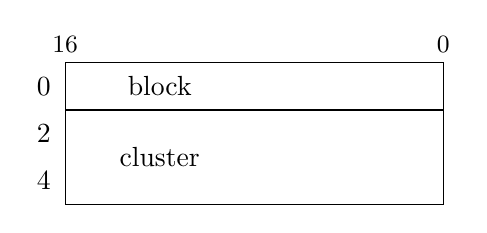
\begin{tikzpicture}[scale=0.3]
  \draw (0,0) rectangle (16,-6);
  \draw (0,-2) -- (16,-2);
%
  \node[anchor=east] at (-0.2,-1) {0};
  \node[anchor=east] at (-0.2,-3) {2};
  \node[anchor=east] at (-0.2,-5) {4};
  \node[anchor=south] at (0,0) {\small 16};
  \node[anchor=south] at (16,0) {\small 0};
%
  \node at (4,-1) {block};
  \node at (4,-4) {cluster};
\end{tikzpicture}

The fields are defined as follows.

\begin{description}
  \item[block] index of the block within the cluster; for instance, with
    four FAT blocks per cluster, this field is in the range 0--3.
  \item[cluster] 32-bit number of the cluster within the filesystem,
    using the FAT filesystem's standard indexing in which the first valid
    cluster is number 2.
\end{description}

Some of the driver's internal subroutines take a pointer to a CABA as an
argument.

Below the level of the CABA, the firmware makes use of a buffer pool that
caches either FAT blocks or drive blocks.  The init\_buffer\_pool subroutine
initializes or reinitializes this pool, using memory allocated on the stack,
as many buffers as will fit while leaving a small allowance for other uses
of the stack at the end of RAM.  Requests for a block through
get\_fat\_block and get\_drive\_block check the cache first and go to the
USB device only if the block was not already cached, with a simple cache
replacement policy.

\section{USB device simulation (overview)}

Testing the FAT filesystem code on real hardware is tricky, especially with
respect to unusual barely-standard flash drive hardware and FAT parameters,
because on top of the usual issues of trying to single-step the
microcontroller without the USB device giving up, unusual hardware is by
nature hard to find.  Generating FAT images with oddball parameters is a
little easier because that can be done in software, but doing it reproducibly
is not easy on every development machine, and loading the oddball images
into the barely-standard flash hardware may present additional difficulties.

So to make debugging easier, the USB mass storage driver has a built-in
simulation feature.  When SIMULATE\_USB\_MASS is defined in config.inc with
an integer from 1 to 6, after boot-up instead of going into the main loop in
firmware.s, the firmware will jump into the USB mass storage driver; and
whenever it tries to read from the mass storage device, it will instead read
canned data from program memory.  The file simdrive.inc sets up the program
memory data for one of six test cases selected by the SIMULATE\_USB\_MASS
value as follows.

\begin{description}
  \item[1] 32G USB stick with FAT32 filesystem in a partition, 512-byte
    drive and FAT blocks, 16K cluster size, some unusal parameters because
    it was formatted by the Windows 10 upgrade process, target file
    unfragmented but deep in the partition so that cluster indices will exceed
    16-bit range.
  \item[2] 80M drive with FAT32, 512-byte drive and FAT blocks, 512-byte
    cluster size, target file heavily fragmented.
  \item[3] 20M drive with FAT16, 512-byte drive and FAT blocks, 1K clusters.
  \item[4] 80M drive with FAT16, 512-byte drive blocks, 2K FAT
    blocks, 8K clusters.
  \item[5] 360K drive with FAT12 (simulating floppy disk), 512-byte drive and
    FAT blocks, 1K clusters.
  \item[6] 1440K drive with FAT12, 2K drive blocks, 1K FAT blocks, 1K
    clusters.
\end{description}

There is a list of blocks hardcoded into the simdrive.inc file for each test
case, and the data for each block of the FAT infrastructure is loaded from
files named like fat32a.bin, fat32b.bin, fat16a.bin, and so on.  These files
are provided in the source package inside simdrive-images.zip.  Be aware
that that file is heavily compressed, containing about 182M of image files
mostly full of zeroes; unpacking it is only recommended if you actually
intend to use the drive-simulation feature.
The data bytes for the simulated firmware image file are extracted not from
the disk images but from simdrive.bin, which is a copy of the current
firmware automatically created by the Makefile as a side effect of doing a
regular build.

When the firmware attempts to read a block in simulation mode, it scans the
list of block numbers, and if the desired block number is found, it then
reads the associated data from program memory.  The consequence of this
design is that the list in simdrive.inc of blocks to be stored for a test
case needs to contain all the blocks that the firmware will attempt to read
while running the test case.  If firmware bugs cause it to read unexpected
blocks, or if the fat*.bin file contents change in a way that points it to
unanticipated block numbers, then the simulated drive will be unable to
return a result for a read call and the firmware will crash in the debugger. 
But as supplied, with the fat*.bin files included with the source, all six
test cases should be able to run as far as starting the loader.

The loader cannot actually succeed with a simulated USB flash drive because
if running in Microchip's simulator, there will be no SRAM to provide data
to the loader; and even if running in real hardware, the entire firmware
image is not actually stored in the simulated drive (simdrive.inc just
folds over the first 8K bytes to make up the size), and so a CRC32 checksum
will probably fail in the loader.  The simulation is only intended for
checking the FAT code.

The file fat32a.bin was created by hand-selecting a few blocks from a FAT
image full of Windows update files that I can't share in full (and it would
be 32G anyway, which is a lot to share).  The others were created by the
included mksimdrives script and in principle could be re-created by running
that script again.  But be careful: first, this script must run as root and
on a Linux system, because it mounts and unmounts loopback image files using
Linux-specific commands.  Also, although it is fairly consistent on my
installation as long as the firmware image size does not change, it is quite
likely that re-running it after any development has occurred will produce
slightly different images, with file blocks in different locations within
the images, so that the block numbers in simdrive.inc may need to be patched
up by hand for the test cases to work after re-running it.  The mksimdrives
script is included primarily for reference and actually running it is not
really recommended.  At the very least, \emph{as with any root script}, you
should go through it, edit it to put in your preferred pathnames, and make
sure you understand how it works, before running it as root on your system.

The remainder of this chapter describes the source code of the driver, which
talks to the USB flash drive using the USB Mass Storage and SCSI commands,
reads drive blocks, breaks or joins them into FAT blocks, and decodes the
FAT filesystem format.  The sections of documentation are arranged in the
same sequence as the code, which may not be the easiest sequence for
understanding the layers of abstraction involved.  Refer back to the
conceptual material above as needed for the description of the data
structures.

\section{TPL entry and RAM data}

Like most Gracious Host per-device drivers, the source file starts with a
TPL entry and some data structures defined in the common data area.  The TPL
entry for this driver is set up to recognize devices exposing an interface
descriptor of USB class 8 (``mass storage''), subclass 6 (``SCSI''),
protocol 80 (``bulk-only'').

The common data area is laid out as required by FIND\_IN\_OUT\_ENDPOINTS
(reused from qwerty.s), with pointers to the first in and out endpoints
at the very start of the common data followed by an array of EP data
structures.  In this case there are just two EPs in the array; we expect the
device to expose exactly one in and one out endpoint.  After that the code
reserves separate IRPs for CBW, CSW, and data transfers, so that we can
avoid needing to reinitialize a shared IRP for these different uses.  See
the USB mass storage overview above.

The rest of the common data variables generally relate to block buffers and
decoding the partition table and FAT filesystem.  They will be described as
they are used.

\section{Driver init}

Unlike most per-device drivers, this one has no ``main loop''; it
unconditionally does its work and then starts the loader instead of
retaining control indefinitely.  At the entry point usbmass\_driver, it
starts by calling USB\_CONFIGURE\_DEVICE to select the configuration and
then FIND\_IN\_OUT\_ENDPOINTS (from qwerty.s) to determine which nedpoint is
the input and which is the output.  Both must exist; if not, the driver
terminates with a THROW.

This driver uses the PRNG subsystem (for CBW/CSW tags), so it calls
START\_CRC to initialize that, and makes a PRNG\_HASH\_TIMERS call at the
start as well to make sure there is at least a little bit of entropy in the
pool.

The first SCSI command sent to the flash drive is READ CAPACITY (10), which
gets the drive's block size and number of blocks.  The code calls
set\_up\_cbw with appropriate parameters to set up the data structures for
this command, then wait\_and\_hash to send it to the device.  These
subroutines are defined later in the file.  The data block for this command
is eight bytes; the code calls transfer\_and\_check\_csw to complete the
command.  If SIMULATE\_USB\_MASS is defined, then a block of code at this
point fills in simulated values for the block size and number of blocks.

Next are some checks for acceptable values returned from the drive.  Drives
greater than $2^{32}$ blocks in size (2T if the blocks are 512 bytes) need a
different command to read their true sizes; they return a last-block index
of 0xFFFFFFFF with READ CAPACITY (10).  The code checks for that value and
THROWs if it is seen; the Gracious Host does not work with drives bigger
than the 32-bit limit.  Next, it confirms that the block size is less than
64K.

The initialization section ends with a call to init\_buffer\_pool, which
sets up the cache to use a block size matching the drive's.  This decision
may be changed later if FAT blocks turn out to differ in size from drive
blocks.

\section{Reading the FAT superblock}

The driver will look for a FAT superblock in up to five places:  block~0,
and the four blocks pointed to by the primary partition table entries, which
are stored in block~0.  In order to reuse the code that checks for a
superblock, these checks are structured so that ``starting in block~0
without a partition table'' is treated as an entry at index $-$1.  The
initialization code sets the partition\_table variable, a 32-bit block index
for the start of the partition currently under consideration, to zero and
the partition\_entry variable, which is the byte offset into block~0 of the
current partition table entry, to one entry length \emph{before} the start
of the table.  It calls get\_drive\_block to load block~0, leaving the
block's data in a buffer pointed to by W4.  Then it continues into
try\_fat\_superblock, which is the return point for the loop.

At try\_fat\_superblock it is assumed W4 points to a buffer containing what
we hope will be the first block of the FAT filesystem.  Valid FAT
filesystems start with magic numbers: either 0xEB in the first byte and 0x90
in the third byte, or else just 0xE9 in the first byte.  These are the
signatures of 8086 assembly language instructions expected to occur at the
start of the PC boot loader code.  The code checks for these and if neither
is found, it branches to try\_next\_partition, which is the increment
portion of the loop, described below.

With a valid magic number match, the next step is to get some metadata from
the superblock: the FAT block size, number of blocks per cluster, count of
reserved FAT blocks at the start of the filesystem before the FAT per se,
and number of root directory entries.  The number of root directory entries
is used for recognizing FAT32, because it is zero for FAT32 (root directory
in a cluster chain, no fixed limit on entry count) and nonzero for FAT12 and
FAT16.

In the FAT32 case, it branches to fat32\_read\_metadata for FAT32-specific
handling of the metadat.  Otherwise, it gets the total number of FAT blocks
(size of the filesystem), which may be stored in one of two fields depending
on whether it first in 16 bits or needs an extended 32-bit field.  It also
gets the number of FAT blocks in each FAT per se.  There follow some
calculations on the metadata values aimed at computing the value for
clusters\_start, which represents the base for indexing into the
filesystem's cluster area.  The smallest valid cluster number is 2 (values 0
and 1 are reserved), but clusters\_start represents the FAT block number
where an hypothetical cluster number~0 \emph{would} start.  Then the
starting point of a given cluster can be calculated as clusters\_start plus
the index times the number of FAT blocks per cluster.  Also calculated along
the way are rootdir\_block, representing the start of the root directory,
and cluster\_limit, representing the smallest \emph{invalid} cluster number.

The cluster\_limit value is used to determine whether this is a FAT12 or a
FAT16 filesystem.  According to the rules documented by Microsoft,
cluster\_limit$>$4086 (approximately 2M when using 512-byte blocks) implies
FAT16 and anything smaller is FAT12.  Some implementations may misbehave by
using the wrong FAT version for filesystem sizes close to this boundary, but
we do not have a better way of determining the version, and the question is
unlikely to come up often in practice.

After recording the FAT version in the fat\_type variable, the code calls
init\_buffer\_pool again to make sure the buffers are big enough to hold
entire FAT blocks, which could be a change from the previous size if FAT
blocks are bigger than drive blocks.  Then it continues into
fat1216\_rootdir\_block\_loop, which loops over the blocks of the root
directory and then over the 32-byte dirents within the blocks.  For each
dirent it calls look\_at\_dirent to see if the dirent is the file we are
looking for.

The loop at fat1216\_rootdir\_block\_loop is unconditional and looks
infinite at first glance, but in fact look\_at\_dirent keeps track of the
number of dirents it has seen and once it reaches the root directory length,
it will branch to try\_next\_partition, ending the loop.  This code path
leaves a superfluous return address on the stack, but it can occur at most
four times in an eventually-successful run, limiting the leak to a
negligible 16 bytes (else the driver would eventually THROW and reset the
stack anyway).

For FAT32 filesystems, the metadata-reading code continues at the label
fat32\_read\_metadata.  It loads several metadata fields from the
superblock, including the number of FAT blocks in the filesystem, number of
FAT blocks in each FAT per se, and the cluster number of the start of the
root directory's chain.  It constructs a CABA for the first block of the
root directory.

Next, it computes the clusters\_start value, much as in the FAT12/16 case
although the calculation is more complicated because of the longer integers
involved.  As in the FAT12/16 case, it calls init\_buffer\_pool again to
make sure the buffers are big enough to contain entire FAT blocks, bearing
in mind that FAT blocks may be bigger then drive blocks.  Then it continues
into fat32\_rootdir\_block\_loop.

The code at fat32\_rootdir\_block\_loop loops over the root directory,
calling look\_at\_dirent for each 32-byte dirent.  It differs a bit from
fat1216\_rootdir\_block\_loop because it needs to use get\_caba to retrieve
blocks of the root directory, and increment\_caba to find the next block
after each one, instead of just reading consecutive FAT blocks.  It also
forces num\_dirents to 0xFFFF each time through the loop to prevent
look\_at\_dirent from ever detecting the end of the directory (which is of
unlimited length in the FAT32 case).  Instead of leaving that to the inner
call, this loop uses the return status of increment\_caba (LE status at the
end of the chain) to recognize when it has reached the end of the root
directory, in which case it will fall through into try\_next\_partition.

\section{Handling the partition table}

The code at try\_next\_partition retrieves the next partition table entry. 
On the first pass through the loop, after looking for a filesystem starting
in block~0, the index variable will have been set up so that the ``next''
partition table entry found by this code is actually the first one.

The code adds 16 bytes (the size of a partition table entry) to the variable
partition\_entry, and then compares it against the address at the end of the
table.  A match indicates we have looked in the whole disk and all
four primary partitions without finding a firmware update image; in that
case the driver terminates with a THROW.

Otherwise, the code calls get\_drive\_block for block~0 to retrieve the
partition table, and checks for the so-called ``boot signature'' value
0xAA55 (little endian) at offset 0x01FE, which refers to the last two bytes
of the block if the block size is the usual 512 bytes.  Failing to find that
value means this is not a standard DOS-style partition table, and the driver
terminates with a THROW.

Next come some checks on the specific partition table entry pointed to by
partition\_entry.  Its type must be nonzero, and its starting block number
must be nonzero.  Failing either check results in a branch back to
try\_next\_partition; this entry is skipped but the table may still have a
usable entry in one of the other slots.  If the table entry looks valid,
then the code saves the partition's starting block number to
partition\_start, loads that first block with a call to get\_drive\_block,
and branches back to try\_fat\_superblock to evaluate whether this partition
may contain a readable FAT filesystem.

\section{Handling a directory entry}

The subroutine starting at look\_at\_dirent examines one FAT directory entry
and does whatever is appropriate for it.  In the current firmware, that
consists of simply checking whether the dirent's filename is FIRMWARE.FRM,
then loading the file contents to SRAM and invoking the firmware loader. 
But this would be a reasonable place to add additional code for doing other
things with other files.

On entry to look\_at\_dirent, W4 should be pointing at a block buffer and
dirent\_in\_block should be the offset into that block of the dirent to look
at.  It starts by scanning the filename, which is in the first 11 bytes of
the dirent, and checking whether it matches the constant string
``FIRMWAREFRM'' (the dot before the extension is implicit).  If the filename
does \emph{not} match, it branches to look\_at\_next\_dirent.  The code
there starts by incrementing dirent\_in\_block 32 bytes, then checks the
number of remaining dirents in the directory (only relevant for FAT12 and
FAT16; the FAT32 calling code defeats this check).  If there are no more
dirents in the directory, it branches to try\_next\_partition, having
completed the scan of the current filesystem.  Otherwise, it checks for the
end of the block and clears dirent\_in\_block if it has reached the end of
the block, before returning.  The logic before the \insn{return} is arranged
so that the CPU status left by the end-of-block check is left in place; the
calling code can use \insn{bra gtu} to detect whether there are more entries
in the current block.

In case of a filename match:  the driver has found its target, a loadable
firmware image file.  It must copy the contents of that file to SRAM.  So it
sends a RSTIO transaction to the SRAM to make sure it is not in some unusual
mode, then initializes a CABA pointing at the start of the file using the
first-cluster number from the dirent.  It resets the 32-bit (only 17 bits
used) variable sram\_pointer to zero, and sends a WRMR command to the SRAM
to put it in sequential mode.

There follows a loop over all the blocks in the file.  The code calls
get\_caba to load one block, opens an SPI transaction and starts a WRITE
command with the SRAM, then sends all the bytes of the block to the SRAM. 
It closes the transaction, updates pointers, and calls increment\_caba to
find the next block in the file.  That subroutine returns GTU status if
there is another block in the file at all, and the loop uses that status for
detecting termination.  Once the file is complete, it removes the stack
frame with \insn{ulnk} and branches to LOADER\_INIT to handle the new
firmware.

\section{Following the FAT chain}

The driver needs to follow FAT chains in two places:  reading the root
directory of a FAT32 filesystem, and reading the actual file contents once
the update image file has been found.  These cases share the
increment\_caba and get\_caba subroutines, which work on the CABA (Cluster
And Block Address) structures described earlier.  Both subroutines take the
addess of the CABA structure as an argument in W2.  They call
the lower-level get\_fat\_block subroutine to do the detail work of finding
a FAT block within the current partition, translating it to one or more
drive blocks, and actually getting the drive blocks.

Part of the reason for this level of abstraction is because
clusters are usually bigger than one FAT block and may often be bigger than
all of the microcontroller's data memory.  It is not enough to just have a
routine for loading a cluster, because a whole cluster might not fit in
memory.  A single FAT block is always expected to fit in a buffer
-- even if it in turn corresponds to more than one drive block.

The code to look up clusters in the FAT per se is in increment\_caba.  It
starts by incrementing the block number within the cluster.  If the result
is within the number of blocks per cluster, then nothing else need be done,
and the subroutine returns, with the GTU (greater than, unsigned) status
from the comparison still in force for detection by the caller.  This
subroutine returns LEU status (less than or equal, unsigned) at the end of
the file, GTU otherwise.

In the case where the increment passed the end of the cluster, it will be
necessary to do a lookup in the FAT per se for the next cluster number.  The
first step is to calculate the byte offset into the FAT of the relevant
entry.  That is the current cluster number times $3/2$, 2, or 4, depending
on whether the filesystem is FAT12, FAT16, or FAT32.  The byte offset
divided by the FAT block size gives the index of the desired FAT block
within the FAT per se; then adding the fat\_start value gives the block
number within the partition, which is the argument for the get\_fat\_block
call that gets the appropriate block of the FAT per se.

Within the block, the remainder from the division by fat\_block\_size gives
the byte offset of the entry.  The code splits here into cases for even and
odd FAT12 entries; FAT16 entries; and FAT32 entries, but the overall effect
in each case is to load the entry value (clearing some reserved bits for FAT32)
into the cluster number of the CABA.  The entry value represents the index
of the next cluster to read.  There are some checks for whether the cluster
number is invalid, which results in a THROW, or is an end-of-chain marker, in
which case the subroutine returns with LEU status to indicate the end of the
file.  Otherwise, it returns with GTU status.

The get\_caba subroutine is simpler.  It just does some double-precision
arithmetic to calculate the FAT block number corresponding to the CABA
(cluster number times fat\_blocks\_per\_cluster, plus block within cluster,
plus clusters\_start) and then falls through into get\_fat\_block.

\section{FAT-level block loading}

Requests for FAT blocks go through get\_fat\_block, which is a simple
wrapper for get\_drive\_block that handles the possible difference in block
sizes.  The buffers are assumed to have been sized for the larger of the two
blocks, and the code checks fat\_blocks\_per\_buffer, which was set while
reading the FAT superblock, to see which is larger.

For FAT blocks strictly smaller than drive blocks, it may be necessary to
find the desired FAT block in the middle of a drive block.  The code does a
$32\times16\rightarrow32$ division to find the drive block number within the
partition, and multiplies the remainder by fat\_block\_size to get the
offset into the drive block.  Then it rejoins the main flow.

For FAT blocks equal to or larger than drive blocks, the offset is always
zero and the code does a multiplication to find the drive block number
within the partition for the start of the FAT block.  In the common case of
FAT blocks and drive blocks the same size, this is a multiplication by 1.

Either way, the partition\_start value is added to the drive block number
(within partition) to get the drive block number (within drive), and the
result is passed to get\_drive\_block.  A final addition adjusts the buffer
address in W4 to account for the offset within the drive block.  Note that
get\_drive\_block actually gets an entire buffer, even if that is more
than one drive block, so the case of a FAT block bigger than a drive block
is covered.

\section{Drive-level buffer pool}

The init\_buffer\_pool subroutine sets up the pool of buffers used for
caching drive and FAT blocks.  The buffers go into a new
\insn{lnk}/\insn{ulnk} stack frame.  The new frame replaces the one set up
by the caller, and the caller must have one in place (and nothing else on
the stack on top of it) before calling this subroutine.  The number of
blocks is chosen to fill the stack, leaving at least STACK\_RESERVATION
bytes free, while not exceeding MAX\_BLOCK\_BUFFERS.  The value of
STACK\_RESERVATION is set in global.inc at 256; and the value of
MAX\_BLOCK\_BUFFERS is set in this file at 24, calculated to represent the
largest number of buffers we could possibly fit in data memory given the
space occupied by fixed-length and fixed-location structures and a minimum
likely block size of 256 bytes.

Buffers are actually allocated eight bytes longer than requested
(BUFFER\_SAFETY\_MARGIN plus rounding) to handle the USB hardware's DMA
overrun.

The buffer\_info variable is an array of six-byte entries that stores
information about the buffers.  Each entry starts with a 16-bit pointer to
the buffer in data memory, and then the remaining 32 bits are the drive
block number of the start of the buffer, or 0xFFFFFFFF if the buffer is
unoccupied.  After the last valid buffer is an entry with a zero in the
address pointer, and there are an extra two bytes at the end of the array to
hold this zero sentinel if all MAX\_BLOCK\_BUFFERS exist.

So the init\_buffer\_pool call sets up this structure.  It begins by
comparing drive\_block\_size against the requested block size in W2, which
will be the FAT block size while processing a FAT filesystem, but another
copy of the drive block size when reading raw drive blocks for the partition
table or FAT superblock, before the FAT block size is known.  The code
splits into two cases to find the ratios fat\_blocks\_per\_buffer and
driver\_blocks\_per\_buffer, at least one of which will be 1.  (More
complicated ratios like 3:2 are not possible because FAT and drive blocks
are both constrained to be powers of two.)  The buffer\_size variable is set
to whichever block size is larger.

Then the code handles re-arranging the stack.  First it pops the caller's
return address into W3, then it removes the old stack frame with \insn{ulnk}
and creates a new, empty one with \insn{lnk}~\#0.  The stack pointer will be
changed later to allocate more bytes.  It computes the available space on
the stack, with the necessary allowances, and divides to find how many
buffers it can allocate.  It throws an exception if there is not room for
even one buffer.

Possibly worth mentioning is that the toolchain provides symbols named
\_\_DATA\_LENGTH for the length of RAM in data memory (expected to be 8K,
0x2000), and \_\_DATA\_BASE for the start of the RAM area after the SFRs
(expected to tbe 0x0800), but the assembler cannot use \emph{both} of these
in the same constant expression, probably because of limitations on how
complicated a ``fixup'' it can pass to the linker to resolve.  So the code
uses a hardcoded value of 0x0800 instead of \_\_DATA\_BASE in this
calculation.

Then it resets next\_victim, a variable used in the replacement policy and
discussed below.  It allocates the buffers as calculated on the stack,
updating the stack pointer to be after them.  It writes the addresses of the
new buffers into buffer\_info, with the unused-buffer marker value of
0xFFFFFFFF in the block number for each one, and a zero address after the
last valid buffer.  Finally, it returns to the caller with a \insn{goto} to
the previously-saved return address.

The get\_drive\_block subroutine is responsible for obtaining a full buffer
that starts with a chosen drive block number, whether that happens by
actually loading it from the drive or by finding such a buffer already in
the cache.  Note that unlike get\_caba, this code requires the requested
block to be at the \emph{start} of the buffer; it will not look for the
requested block in the middle of a buffer.

It starts by a straightforward scan of the buffer\_info data structure for a
buffer whose block number matches the request.  If found, that block will be
the return value; but before actually returning it, the code falls through
into find\_new\_victim to maintain the cache replacement policy before
returning.

Now, about the cache replacement policy.  The basic concept here is that
requests for blocks could come in in any order.  If a block is not in the
cache, then (except for a brief time at the start while there exist
never-used buffers) we must evict a block currently in the cache to make
room for the new one.  Ideally, we should evict a block which we will never
need again; failing that, one we will not need soon.  We want to keep
frequently-used blocks in the cache and evict rarely-used ones, so that
future requirements to reload blocks will be minimized.
It is not possible for a cache replacement policy to be optimal on all
possible sequences of block requests because it would have to know the
future; but some carefully-designed policies can come close to the
theoretical limits.

The Gracious Host USB mass storage driver uses a very simple policy
that seems to work well in practice and is basically a modification of the
well-studied ``Clock'' algorithm.  It keeps a variable called next\_victim
which is a pointer to what will nominally be the next block buffer used by a
new block.  When get\_drive\_block cannot find a block in the cache and
needs to load it from the drive, it will load the new block into the buffer
designated by next\_victim, evicting whatever was there before.

However, whenever get\_drive\_block returns a block, it checks whether that
block happens to be the next\_victim block (always true after a cache miss,
sometimes true after a cache hit).  In such a case, next\_victim is
incremented to the next buffer, wrapping around at the end of the array.  So
accessing a block that was about to be evicted gives it a reprieve until the
pointer rotates all the way around the array again.  During startup, when
the block buffers are all empty, next\_victim will advance to a new empty
block as each one is filled.  If there should happen to be only one buffer,
next\_victim remains on that buffer and the buffer gets reloaded frequently.

On a cache miss, when the code was unable to find the block already
buffered, it saves the next\_victim pointer to W4 and then calls
find\_new\_victim to increment it.  The find\_new\_victim subroutine has the
side effect of replacing W4 (pointer to buffer\_info entry) with [W4]
(pointer to the actual block buffer).  The cache miss code saves that buffer
into the buffer field of data\_irp, to be the destination of the upcoming
read from the drive.

Then it prepares a CBW for the SCSI READ (10) command, to cover a range
of blocks starting at the requested drive block number and covering the size
of a buffer (one or more drive blocks).  This setup includes a call to
shared code in set\_up\_cbw to prepare fields, in particular the tag field,
common to all CBWs.  Then it calls wait\_and\_hash to send the CBW to the
device, and transfer\_and\_check\_csw to do the data transfer and process
the terminating CSW.  It recovers the buffer address from the IRP and
returns it.

In the case of device simulation:  the calls to read the data are executed
but have no hardware effect because the instructions that would touch the
hardware are removed by conditional assembly.  Then just as
get\_drive\_block is about to return in the cache miss case, there is an
added call to simulate\_block\_read, which will copy data from the simulated
drive into the buffer.

\section{USB communication}

Subroutines in this section of the source file abstract much of the CBW/CSW
handling needed throughout the USB mass storage protocol.  First,
wait\_and\_hash is just two instructions that call USB\_WAIT\_ON\_IRP to do
a low-level USB transaction, then tail-call PRNG\_HASH\_TIMERS. 
Higher-level code in the mass storage driver usually uses this instead of
just calling USB\_WAIT\_ON\_IRP, so that the PRNG will continue being
re-seeded with timing information from the USB transactions.  The
USB\_WAIT\_ON\_IRP call here is conditional on SIMULATE\_USB\_MASS
\emph{not} being defined, so the USB communication will be skipped in
simulation mode.

The set\_up\_cbw subroutine does most of the setup for the CBW phase of a
mass storage command.  It writes the magic number into the cbw\_buffer
variable, gets a 32-bit random tag from the PRNG and stores that both in the
buffer and the xaction\_tag variable for future checking, zeros most fields
and puts the necessary values in a few that need to be non-zero, and sets up
W1 and W2 for an upcoming call to wait\_and\_hash.

The transfer\_and\_check\_csw subroutine handles the rest of the mass
storage command (data and CSW phases); it is separated from set\_up\_cbw to
allow different callers to do command-specific buffer setup before the data
and CSW phases.  The code starts with a call to wait\_and\_hash for the data
phase.  Then it sets up csw\_irp and the associated buffer for the 13-byte
CSW transfer and calls wait\_and\_hash again to do that transfer.

There follow a bunch of checks on the data returned in the CSW.  All the
checking code is conditional on SIMULATE\_USB\_MASS being undefined; in
simulation mode, the subroutine just returns.  But when not in simulation
mode, it checks that the CSW magic number is correct; that the random
transaction tag matches the one stored in xaction\_tag; that the length of
the data transfer was as requested; and that the result code was successful. 
If any of these checks fail, it will THROW instead of returning.

\section{USB device simulation (support code)}

The simulate\_block\_read subroutine, which is assembled at all only in
simulation mode, runs at the end of get\_drive\_block to fill in the buffer
contents that were not written by the skipped code to read from the drive. 

This code starts by extracting the block index that the caller was asking
for, from the CBW buffer.  Then it scans the table in program memory at
\_block\_tbl for an entry matching the requested block.  If no match, it
crashes into an infinite loop, which provides a convenient place for the
debugger to break if running in a debugger, and will eventually lead to a
WDT timeout if running on real hardware.  In case of a match, it copies the
data from program memory to the buffer and then returns.


% $Id: glossary.tex 9823 2022-02-09 01:07:30Z mskala $

%
% Glossary for MSK 014 programmer's manual
% Copyright (C) 2022  Matthew Skala
%
% This program is free software: you can redistribute it and/or modify
% it under the terms of the GNU General Public License as published by
% the Free Software Foundation, version 3.
%
% This program is distributed in the hope that it will be useful,
% but WITHOUT ANY WARRANTY; without even the implied warranty of
% MERCHANTABILITY or FITNESS FOR A PARTICULAR PURPOSE.  See the
% GNU General Public License for more details.
%
% You should have received a copy of the GNU General Public License
% along with this program.  If not, see <http://www.gnu.org/licenses/>.
%
% Matthew Skala
% https://northcoastsynthesis.com/
% mskala@northcoastsynthesis.com
%

\chapter{Glossary}

\begin{description}

\item[absolute section] to the disappointment of tsundere fans, this is a
reserved section in object code files used for storing symbols whose values
are just unrelocatable numbers and not offsets into memory sections that the
linker should relocate.  The\ .struct assembler directive is documented
(sketchily) as being for defining symbols in the absolute section that can
then be used as offsets into data structures; but it either was broken by
Microchip when they did their chop job on the GNU assembler, or it may have
never even worked in the original GNU assembler to begin with.

\item[ADC] Analog to Digital Converter, a device that converts voltage
measurements to digital numbers.  The Gracious Host uses a 10-bit ADC that
is built into the microcontroller.

\item[API] Application Programming Interface, the interface through which
application software can make use of a library or driver.

\item[BCD] Binary Coded Decimal:  decimal translated to binary by
translating each digit to four bits independently, rather than using the
integer value of the entire number at once.  Basically the same
thing you would get by pretending the decimal number is actually hexadecimal.

\item[big endian] handling the most significant bytes of a multi-byte number
first, or storing them in smaller-indexed addresses.  Some computers, and
almost all Internet-associated protocols, prefer big endian, hence the
alternate name \emph{network byte order}.  See also \emph{little endian}. 
The USB Mass Storage specification, in its most popular variation, requires
both big endian and little endian numbers in different parts of the same data
structures.

\item[bit bang] serial communication by means of software on the CPU
controlling the timing of individual bits on one or more GPIO pins, instead
of using a specialized peripheral that implements the serial protocol in
hardware.

\item[boot keyboard] the USB Human Interface Device Specification's name for
the ordinary kind of typing or QWERTY keyboard typically used with PCs, and
the protocol for talking to it; called \emph{boot} because of their idea
that this protocol would only be used during the boot sequence and then
would be replaced by something more complicated once the full operating
system finished loading.

\item[boot mouse] much like \emph{boot keyboard}, the basic low-feature and
low-complexity USB mouse protocol.

\item[CABA] Cluster And Block Address, a data structure specific to the
Gracious Host FAT filesystem driver, used for referring to blocks within
chains.

\item[CBD] Technically this is the abbreviation for cannabidiol, a drug
found in cannabis and purported to have health benefits while producing
little or none of the ``high'' produced by tetrahydrocannabinol (THC); but
in the context of USB Mass Storage, more likely a typo for CDB.

\item[CBW] Command Block Wrapper.  A 31-byte structure sent from host to
device to initiate a USB Mass Storage bulk-only SCSI command.  Contains an
unaligned 16-byte field for the SCSI CDB.

\item[CDB] Command Data Block.  The header of a SCSI command, likely
to be followed by a data transfer in one direction or the other.  Tends to
contain big-endian fields with 16-bit alignment.  SCSI commands are often
named with the length of the CDB, with more than one length and CDB layout
possible for what would otherwise be the same command, such as READ (10) or
READ (12).

\item[CSW] Command Status Wrapper.  A 13-byte structure sent from device to
host after completion of a USB Mass Storage bulk-only SCSI command to report
success or failure of the command and maintain synchronization.

\item[cluster] in a FAT filesystem, the unit of allocation.  A cluster may
be from 1 to 64 \emph{FAT blocks}; standard FAT filesystems have the
limitations that the cluster size must be a power of 2 and no more than 64K
bytes total (no more than 16K in many implementations), but the Gracious
Host can actually read some filesystems that break those rules.

\item[common data] a toolchain feature by which copies of a symbol can be
defined in more than one assembly-language file and will then be merged to
all appear at the same address; not perfectly supported by the
PIC24 toolchain, but we use it to implement a substitute for the even more
broken \emph{data overlay} feature.

\item[CN] Change Notification, a microcontroller feature that allows a GPIO
pin to serve as an interrupt request.

\item[CPU] Central Processing Unit.

\item[CRC] Cyclic Redundancy Check, a kind of checksum based on finite field
polynomial division; our microcontroller has a dedicated hardware module for
computing these efficiently.

\item[CRC32] One of:  the PIC24F peripheral for calculating CRCs; a specific
very popular 32-bit CRC algorithm used by the Gracious Host for checking the
integrity of firmware update images and in the PRNG code; or just any 32-bit
CRC.

\item[CRC5] a specific 5-bit CRC algorithm used in USB for low-level bit
error detection and affected by a silicon erratum in the PIC24F USB
hardware.

\item[CTMU] Charge Time Measurement Unit, a microcontroller feature for
implementing capacitive touch controls, not usable in the Gracious Host
hardware.

\item[CV] Control Voltage, as in a Eurorack synthesizer patch.

\item[DAC] Digital to Analog Converter; the Gracious Host contains a
separate 12-bit two-output DAC chip connected to the microcontroller
by the SPI port.

\item[data overlay] a toolchain feature by which multiple software modules
that will not run at the same time can reuse the same addresses for their
RAM data, saving overall memory consumption; desired by the Gracious Host
firmware but unusable in the PIC24F toolchain because of linker bugs.

\item[descriptor] in USB, a data structure that the device returns to the
host during a configuration phase after enumeration.  Devices usually have
many descriptors, containing information about the device's manufacturer and
model number, which USB standards it supports, its capabilities and
limitations (such as number of buttons or ports), and so on.

\item[dirent] Directory Entry.  A 32-byte record in a FAT filesystem's
directory (root directory or subdirectory).  A basic dirent stores the
8.3-format short filename, file size, starting cluster number, timestamp,
and so on.  Files with longer names have extra dirents each
storing a chunk of the long name.

\item[drive block] my name for a block of data in the native size of a USB
Mass Storage device as reported by the SCSI READ CAPACITY (10) transaction,
used to organize subsequent data transfers.  In practice this is
expected to always be 512 bytes, but the Gracious Host can also handle a few
larger sizes.

\item[DMA] Direct Memory Access, the act of a peripheral reading or writing
general RAM directly instead of going through the CPU and special registers
or memory mapping, often mediated by a \emph{DMA controller}.  The PIC24F
USB module uses DMA with a built-in dedicated controller.

\item[DS] Data Sheet, specifically the \emph{PIC24FJ64GB004 Family Data Sheet}
published by Microchip.

\item[ECPLL] External Clock Phase Locked Loop, the operating mode for the
microcontroller clock used in the Gracious Host.  An external crystal
oscillator module supplies a digital reference at an accurate frequency that
gets multiplied and then divided to generate the different clock frequencies
needed internally by the microcontroller.

\item[enumeration] something that is supposed to happen when a USB device is
attached to a USB host: the host assigns the device an ID number, so
that different devices on the same bus can be addressed separately.  The
Gracious Host tells every device to be number 1, because there can only
be one device attached at a time anyway.

\item[EP] ``endpoint''; a data structure used by the USB driver to represent
the local end of a ``pipe'' between software on the host and a ``function''
on the device.

\item[Fast RC] one of the built-in oscillators on the microcontroller,
capable of running the chip at full speed without needing any external
components, but not accurate enough for USB operation unless possibly it may
be \emph{trimmed} for the variations of individual chips by a fiddly and
poorly-documented procedure.

\item[FAT] File Allocation Table; see \emph{FAT filesystem} and \emph{FAT
per se}.

\item[FAT filesystem] a data structure for storing files and directories on
a disk or a disk-like medium, made popular by MS-DOS, subsequently used by
Windows, and popular for USB Mass Storage devices even when they are read
and written by non-Microsoft systems.  The Gracious Host includes a
low-featured FAT filesystem driver for reading firmware update images from
USB flash drives.  FAT filesystems are described as FAT12, FAT16, or FAT32
depending on the bit width of the entries in the \emph{FAT per se}.

\item[FAT per se] the part of a \emph{FAT filesystem} that is literally
named the ``file allocation table.'' It is an array of entries that are 12,
16, or 32 bits long, recording for each cluster in the filesystem whether
that cluster is in use, bad, or free, and if in use, which other cluster is
next in the chain.

\item[FAT block] my name for one of the blocks used to organize a FAT
filesystem, officially (but confusingly) called a \emph{logical sector} and
not necessarily matching the \emph{drive block} size.

\item[FIFO] First In First Out, describing a type of buffer commonly used
between the CPU and a peripheral, in either direction, so that they will
less often need to wait for each other.

\item[firmware] software that is built into hardware, effectively becoming
part of it.

\item[foreground] the code running on the microcontroller under ordinary
circumstances, when it is \emph{not} processing an interrupt.

\item[FRM] Family Reference Manual, specifically the \emph{PIC24F Family
Reference Manual} published (a chapter at a time, not as a single document)
by Microchip.

\item[GPIO] General Purpose Input/Output, the common digital interface pins
on many microcontrollers.  GPIO pins can usually be configured one at a time
as input or output, and often have some extra features like being
configurable for open-drain or tri-state output modes, or to generate
interrupts in input mode.

\item[GPL] the General Public License, a set of copyright licensing terms
applicable to the Gracious Host hardware and firmware, as well as to the GNU
toolchain.  It means you're allowed to distribute and make modifications to
the things in question, but you're not allowed to prevent others from doing
the same.

\item[hardware breakpoint] in ICD, breakpoints mediated by undocumented
hardware features.  They are efficient and do not wear out the flash, but
you can only have up to four code and four data hardware breakpoints at a
time, and if you use more than three, you lose some single-stepping
capability and the Microchip tools will encourage you to switch to software
breakpoints.

\item[Harvard architecture, modified] a computer architecture that puts code
and data in separate address spaces which may have significantly different
rules, common in microcontrollers too small to run operating systems; used
in PIC24.

\item[HID] Human Interface Device, the USB term for a general category of
devices used by humans to directly communicate with computers.  Includes
mice, typing keyboards, and some things like joysticks, arcade buttons, and
VR controllers, but notably does \emph{not} usually include music keyboards
(which tend to be USB-MIDI instead) nor sex toys (which tend to have
proprietary vendor-only protocols).  The USB HID standard includes
simplified protocols for typing keyboards and mice, which are called the
``boot'' protocols, and a much more complicated generic protocol intended to
work with all types of HIDs including all of their unique features.

\item[ICD] In-Circuit Debugging, with a special hardware device plugged into
reserved pins on the microcontroller to allow stepping through the code,
setting breakpoints, and so on.

\item[ICSP] In-Circuit Serial Programming, loading the microcontroller with
its firmware through basically the same interface as ICD.

\item[I$^2$C] Inter-Integrated Circuit (bus), a serial bus similar in nature
and typical application to SPI, and supported by the microcontroller, but
not actually used in the Gracious Host.

\item[IRP] I/O Request Packet, the USB standards' term for a data structure
passed into the driver when requesting data to be transferred over the bus
in either direction.

\item[ISR] Interrupt Service Routine, the subroutine that handles an
interrupt.  In PIC24 these need to return with the special \insn{retfie}
instruction instead of an ordinary \insn{return}.

\item[keep-alive] a pulse sent from the host to the device at 1\,ms
intervals on a low-speed USB connection.  The device disconnects if it
misses three consecutive keep-alives.

\item[LDO] Low Drop Out, describing a voltage regulator that can operate
with significantly less than the minimum 3V difference between input and
output that is required by traditional 78xx-style regulators.

\item[level-triggered] Microchip's description of the USB attach and detach
interrupts, which will keep reoccurring until fully disabled as long as the
relevant state persists, even if the individual interrupts are acknowledged
in the way required by other PIC24F interrupts.

\item[linker script]  A file that gives the linker instructions on how to
process fragments of code and data into the memory image of the complete
program.  The Gracious Host uses a customized linker script to put knowledge
about drivers into the higher-level code that uses it; but even the default
PIC24 linker script does a lot of complicated processing to support features
like automatic creation of interrupt vector tables, and initialization of
high-level language variables.

\item[little endian] handling the least significant bytes of a multi-byte
number first, or storing them in smaller-indexed addresses.  PIC24
microcontrollers have a preference for little endian organization.  See also
\emph{big endian}.

\item[LSB] Least Significant Bit; the bit with least numerical value,
normally written on the right.

\item[microcontroller] in this manual, specifically the Microchip
PIC24FJ64GB002-I/SP microcontroller.

\item[Microchip Corporation] vendors of PIC24 chips, some other chips used
in the Gracious Host, and hardware and software development tools. 
Distributors of a version of the GNU multi-platform toolchain modified to
work with PIC24, which means they have certain obligations under the GPL. 
See also \emph{Sirius Cybernetics Corporation}.

\item[MIDI] Musical Instruments Digital Interface.

\item[MSB] Most Significant Bit; the one with greatest numerical value,
normally written on the left.

\item[mutatis mutandis] Medieval Latin for ``with the necessary changes.''

\item[OTG] USB On The Go, a specification explaining how a USB host or
device can be confused about which one of those it is.

\item[page] in the context of the PIC24F flash program memory, an aligned
block of 512 words or 1536 bytes; this is the unit of flash erase
operations.

\item[PIC24] Microchip Corporation's 16/24-bit microcontroller architecture.

\item[PIC24F] a specific family of microcontrollers, subset of the broader
PIC24 architecture.

\item[PID] Packet Identifier.  A four-bit code attached to USB packets which
specifies their role in the protocol.

\item[PMP] Parallel Master Port, a feature of some larger PIC24F
microcontrollers that theoretically exists in the silicon of ours too, but
cannot actually be used because of packaging limitations, let alone the
conflicting Gracious Host board design.

\item[polyfuse] a component in the Gracious Host hardware, technically a
special temperature-sensitive resistor, that functions like a fuse to
temporarily shut off power to the connected USB device if the device tries
to draw a dangerously large amount of power.

\item[PPQN] Pulse Per Quarter Note.  Describes the ratio between synthesizer
tempo clock signals and musical notes.  MIDI uses a 24~PPQN clock, meaning
that there are 24 clock pulses for each quarter note.  At a tempo of 120
BPM, the 24~PPQN clock has $120\times 24 = 2880$ pulses per minute, or 48
pulses per second.

\item[PPS] Peripheral Pin Select, a microcontroller feature allowing the
mapping between on-chip digital peripherals and pins of the 28-pin SPDIP
package to be changed under software control.

\item[PRNG] Pseudo-Random Number Generator.  In the Gracious Host this is a
firmware feature implemented in utils.s and used by the MIDI backend for
random arpeggiation and by the USB mass storage driver to generate
transaction-recognition tokens.  It makes use of the CRC32 module.

\item[PSV] Program Space Visibility, a feature of the PIC24 architecture by
which part of program memory can be made to appear in a read-only window of
the data memory space.

\item[row] in the context of the PIC24F flash program memory, an aligned
block of 64 instruction words, equal to 192 bytes; there are 8 rows to
each page, and some flash write operations write a whole row at a time. 
Each set of Gracious Host calibration data uses, though it does not entirely
fill, one row.

\item[SCSI] Small Computer System Interface, originally a parallel bus used
for connecting disk drives and other peripherals to computers; basically
obsolete in its original form, but some more recent standards, including the
common variant of USB Mass Storage supported by the Gracious Host, work by
sending SCSI commands on top of some other protocol.  SCSI is \emph{big
endian}.

\item[SFR] Special Function Register(s); the hardware registers used for
communication with the microcontroller's on-chip peripherals and for CPU
control, mapped between addresses 0x0000 and 0x07FF in data memory.

\item[skinny DIP] a Dual Inline Package (DIP) for a through-hole IC with
0.300$''$ row spacing despite having 24 pins or more.  Traditional DIPs use
0.300$''$ spacing only for packages with fewer than 24 pins and 0.600$''$ at
higher pin counts.  The microcontroller in the Gracious Host comes in a
28-pin skinny DIP.

\item[soft timer] a timer implemented by having the CPU periodically update
a variable in RAM, instead of by using a hardware counter that runs
independently of the CPU.

\item[software breakpoint] in ICD, breakpoints implemented by rewriting the
program memory instead of using the hardware debugging features.  You can
use an unlimited number of software breakpoints, but they are slower, and
they cause significant wear on the flash memory.

\item[SOF] Start Of Frame, a packet the host sends to the device at
1\,ms intervals on a full-speed USB connection, much like the low-speed
\emph{keep-alive}.  The PIC24F hardware can
be set to generate an interrupt linked to the SOF.

\item[SPDIP] Skinny Plastic Dual Inline Package; see \emph{skinny DIP}.

\item[SPI] Serial Peripheral Interface, a serial bus used in
the Gracious Host to control the SRAM and DAC chips.

\item[SRAM] either Serial Random Access Memory or Static Random Access
Memory, which are not the same thing but the 23LC1024 SRAM chip in the
Gracious Host happens to be both.  This chip provides 128K bytes of memory
accessible to the microcontroller via SPI transactions, and is used as
a buffer for the incoming firmware image when updating firmware from USB
mass storage.

\item[star section] a section (in the assembly-language sense) with
its name declared as just an asterisk.  Then the assembler will automatically
give it a unique name, separating it from other sections and allowing
the linker some flexibility in locating it.

\item[tail call]  When a subroutine ends by branching to another subroutine. 
The return from the second subroutine has the effect of returning to the
caller of the first.  If the last instruction of the first subroutine before
returning would have been a regular call to the second subroutine, then
doing a tail call instead saves some time and space.

\item[TDL] Targeted Device List, the Gracious Host-specific term for the
part of the TPL executable data structure that recognizes entire devices
based on the information in their device descriptors.

\item[TIL] Targeted Interface List, the Gracious Host-specific term for the
part of the TPL executable data structure that recognizes interface
descriptors within a device, if no TDL entry has claimed the device first.

\item[TLA] usually read as Three-Letter Acronym, though many including TLA
itself are more properly called Three-Letter \emph{Abbreviations} because
they are not pronounced as words.

\item[toolchain] the sequence of software tools that turn source code into a
loadable binary image.  For PIC24 assembly language programs like the
Gracious Host firmware, the toolchain as such is basically just the
assembler and linker, although side utilities for dealing with object and
archive files are often counted as part of the broader toolchain entity.

\item[TPL] Targeted Peripherals List, the list of USB devices with which a
USB host is intended to work -- both a listing in the documentation and a
data structure likely to exist in its driver software.

\item[trap] basically an interrupt that happens when something really bad
has occurred, like an unaligned memory access.  They cannot be ignored or
masked, and normally lead to a CPU reset.

\item[UART] Universal Asynchronous Receiver Transmitter, a serial interface
traditionally used for connecting to things like modems and terminals.

\item[UBM] the \emph{MSK~014 Gracious Host User/Build Manual}, companion to
this volume.

\item[USB] Universal Serial Bus.

\item[VCO] Voltage Controlled Oscillator.  One of the basic modules in an
analog synthesizer.  Eurorack VCOs in particular usually have their
frequencies controlled by a voltage that shifts the frequency \emph{one volt
per octave} (V/oct); VCOs in non-Eurorack systems may have different control
voltage standards.  One of the main applications for the Gracious Host is in
controlling a VCO, and a V/oct VCO is required for the calibration process.

\item[von Neumann architecture] a computer architecture in which code and
data are in the same address space, accessed in substantially the same way,
typical of general-purpose computers and usually taken for granted by
operating systems and programming language tools.

\item[WDT] Watch Dog Timer, which resets the CPU if the firmware does not
clear the timer occasionally; intended to break out of situations where the
firmware has gone into an uncontrolled infinite loop.  There is also a
\emph{deep-sleep WDT}, not used on the Gracious Host, which has a similar
function in longer-lasting power-saving modes.

\item[ZIF socket] Zero Insertion Force socket, a type of IC socket designed
to withstand many cycles of inserting and removing ICs without damage to
either party, such as in IC testing equipment or for the CPU chip on
a desktop computer motherboard.

\end{description}


%%%%%%%%%%%%%%%%%%%%%%%%%%%%%%%%%%%%%%%%%%%%%%%%%%%%%%%%%%%%%%%%%%%%%%%%

\end{document}
